\documentclass[upright, contnum]{Config/umemoria}

%fix for the oneside argument
\makeatletter
\g@addto@macro\titlepage{\pagenumbering{Alph}}
\g@addto@macro\endtitlepage{\pagenumbering{roman}}
\makeatother

\depto{Departamento de Ingeniería Mecánica}
\author{Iván Ignacio Gonzalez Pérez}
\title{Welding droplet segmentation using Deep Learning}
\auspicio{}
\date{Diciembre 2020}
\guia{Viviana Meruane Naranjo}
\carrera{Magíster en Ciencias de la Ingeniería, Mención Mecánica}
\memoria{Tesis para optar al Grado de \break  Magíster en Ciencias de la Ingeniería, Mención Mecánica \break
\break
Memoria para optar al título de \break  Ingeniero Civil Mecánico}
\comision{Patricio Méndez, Rubén Fernández}



\usepackage[utf8]{inputenc}
\usepackage[T1]{fontenc}


\usepackage{etoolbox}% http://ctan.org/pkg/etoolbox
\makeatletter
% \patchcmd{<cmd>}{<search>}{<replace>}{<success>}{<failure>}
% --- Patch \chapter
\patchcmd{\@makechapterhead}{50\p@}{\chapheadtopskip}{}{}% Space from top of page to CHAPTER X
\patchcmd{\@makechapterhead}{20\p@}{\chapheadsep}{}{}% Space between CHAPTER X and CHAPTER TITLE
\patchcmd{\@makechapterhead}{40\p@}{\chapheadbelowskip}{}{}% Space between CHAPTER TITLE and text
% --- Patch \chapter*
\patchcmd{\@makeschapterhead}{50\p@}{\chapheadtopskip}{}{}% Space from top of page to CHAPTER TITLE
\patchcmd{\@makeschapterhead}{40\p@}{\chapheadbelowskip}{}{}% SPace between CHAPTER TITLE and text
\makeatother
% Set new lengths
\newlength{\chapheadtopskip}\setlength{\chapheadtopskip}{10pt}
\newlength{\chapheadsep}\setlength{\chapheadsep}{20pt}
\newlength{\chapheadbelowskip}\setlength{\chapheadbelowskip}{15pt}


\begin{document}

\frontmatter
\maketitle

\begin{abstract}
{Recently, deep learning models have had an outstanding performance in tasks such as image classification, anomaly detection and natural language processing. These models thrive when the amount of data is large, which is common nowadays. Coupled with the increasing computing power of GPU, it is possible to solve many of otherwise intractable problems. Nevertheless, the deep learning approach has been mainly used in computer vision while other fields have not adopted it as much. Hence, there is an opportunity to use these models to outperform previous results in the welding field.

In the following work the aim is to use deep learning segmentation models to solve the problem of obtaining relevant features of a Gas Metal Arc Welding (GMAW) process. This is done by segmenting video footage to isolate droplets and then calculating features that are relevant to characterize the process. This problem has been addressed before with computer vision techniques, but the methods used lack automation, and processing large volumes of data becomes unfeasible. Therefore, this thesis' approach allows to achieve results in the segmentation problem itself and the automation process, since results can be obtained faster.

The proposed model is a Fully Convolutional Network approach. Several architectures are considered and compared to then use the best one for further calculations, which by means of supervised training can take a large amount of images and return segmentation masks for each one, isolating the droplets from the background. Furthermore, segmentation masks are used to compute geometric and physical properties. This can be helpful to understand and design the welding process, since it would be possible to map the inputs like current, voltage and shielding gas to a measurable output such as position, area, frequency and velocity of droplets.

A literature review is carried out to understand the problem, how it has been addressed so far and to study the approaches for segmentation using deep learning. Then, data is acquired, consisting of videos of GMAW processes depicting globular and spray transfer which are manually labeled and augmented. Later, Fully Convolutional Network based architectures are trained with the labeled data, namely U-Net, DeconvUnet and MultiResUnet. Finally, the resulting segmentation masks are processed to compute geometric and physical properties.

The main conclusion of this work is that the U-Net based approach can reliably segment droplets within a frame, achieving similar results to previous attempts, but with the benefit of being able to process thousands of images in seconds or minutes. Furthermore, relevant properties were obtained, namely position, velocity, acceleration, perimeter, area, volume and surface tension among others, with values mostly in agreement with literature. Hence this work is a successful step towards automation and a better understanding of GMAW.}
\end{abstract}

\cleardoublepage

\begin{abstract}
{Recientemente, modelos de aprendizaje profundo han obtenido buenos resultados en tareas como clasificación de imágenes, detección de anomalías y traducción de idiomas. Estos modelos mejoran cuando hay una alta cantidad de datos, lo que es común hoy en día. Sumado al constante aumento en poder de cómputo de las GPU, es posible resolver problemas que de otro modo serían difíciles o intratables. Sin embargo, el enfoque de aprendizaje profundo se ha aplicado principalmente en visión computacional, mientras que en otros campos de la ciencia no se ha aplicado al nivel que los avances permitirían. De este modo, existe una oportunidad de usar estos modelos y mejorar resultados en nuevos campos del conocimiento. Lo anterior ha ocurrido en algunas disciplinas como lo son la biomedicina, gestión de activos físicos o la química, con excelentes resultados.

En el siguiente trabajo el propósito es utilizar modelos de aprendizaje profundo de segmentación para obtener características relevantes de un proceso de soldadura a gas y arco metálico (GMAW), esto se hace mediante la segmentación de un video para separar a las gotas del fondo y luego calcular características. El problema ha sido abordado con el uso de técnicas de visión computacional, pero las técnicas usadas carecen de automatización, por lo que procesar una gran cantidad de datos se hace inviable. Por lo tanto, el enfoque de esta tesis permite resolver el problema de segmentación en sí, y el problema de automatización, pues los resultados se pueden obtener rápidamente.

El modelo propuesto es una red neuronal tipo U-Net, la cual mediante entrenamiento supervisado recibe imágenes y entrega una máscara de segmentación. Luego, las máscaras se usan para calcular propiedades geométricas y cinemáticas, lo cual es de ayuda para comprender y diseñar el proceso de soldadura, ya que permite establecer una relación entre input como voltaje, corriente o gas protector y output como posición, área, frecuencia y velocidad de las gotas.

La metodología es la siguiente: Primero, se realiza una revisión de literatura para comprender el problema y cómo se ha abordado hasta ahora, y para estudiar propuestas de segmentación de aprendizaje profundo. Segundo, se adquieren datos para un caso de estudio, los datos consisten en videos de procesos de GMAW con modos de transferencia globular y spray. Los videos se separan en cuadros y una porción de ellos es etiquetada. Posteriormente se entrena un modelo tipo U-Net con los datos etiquetados. Tercero, las máscaras de segmentación se utilizan para calcular características como posición, área, velocidad, frecuencia de deposición y frecuencia de oscilación. Finalmente, los resultados se discuten en términos de su confiabilidad y aplicablidad en soldadura.

La conclusión principal de este trabajo es que la propuesta de un modelo tipo U-Net es capaz de segmentar correctamente las gotas dentro de una imagen, consiguiendo máscaras similares a propuestas anteriores, pero con el beneficio de poder procesar una miles de imágenes en minutos. Además, el post-procesamiento es capaz de obtener propiedades físicas del proceso que permiten entenderlo y diseñarlo mejor.}
\end{abstract}

%\begin{dedicatoria} % opcional
%"Stately, plump Buck Mulligan\\came from the stairhead,\\bearing %a bowl of lather\\on which a mirror\\and a razor\\lay crossed."
%\end{dedicatoria}

%\begin{thanks} % opcional

%\end{thanks}


%\tableofcontents
%\listoftables % opcional
%\listoffigures % opcional

\mainmatter

\begin{intro}
\section{Introduction}
%\cite{Duong, Casser, Ronneberger, Long, Noh, Ibtehaz, Ray, Kass, Zhai, Gunther, Zhang, Shi}
The optimization of arc welding processes in general has always been an important task since it is necessary to get better results both in the quality of the joints as well as the efficiency of the process in terms of time and materials to produce durable and reliable results. There are constant efforts in improving the welding machines, using better quality materials, physical modeling of the process and increasing the automation of both the welding itself as well as the design in order to achieve an optimized welding process.

A widely used arc welding technique is the Gas Metal Arc Welding (GMAW) in which a bare metal wire electrode is consumed while a shielding gas floods the area to avoid external contamination \cite{weld-review}. The study of this process is a complex task, since there are many fields involved such as fluid dynamics, heat transfer and solid mechanics. Also, from a technical standpoint there are several parameters that affect the process as a whole, such as voltage and current waveform, material and diameter of the electrode and shielding gas.

One way to approach the study of GMAW in order to better understand and optimize the process is by using data-driven models. These models have thrived in recent years because of the high volume of data that can be collected using a wide range of sensor data such as images, acoustic signal, temperature, pressure, among many others. 

Specifically, deep learning models have been able to solve problems which would otherwise be difficult or intractable. Deep learning models have reached state of the art results in tasks such as image classification, image segmentation, natural language processing and optimal control taking advantage of the large datasets available \cite{dl-review} and advances in hardware. Also, different scientific fields outside of the typical computer vision applications have successfully adopted this approach, such is the case in bio-medicine, prognostics and health management and the mining industry to name a few \cite{Ronneberger, Reza, Jia}.

Furthermore, a data-driven approach for GMAW study poses the challenge of which parameters to measure and how to do it, since the process itself occurs at very high temperatures, it is difficult to use a measuring device directly, because it would need to resist these conditions while functioning optimally as well as not disturbing the process itself.

Therefore, a suitable approach would be to use image data, since the camera can stay away from the process while capturing important information, namely the movement of the welding droplets from the wire to the weld pool. For this, the experimental setup would need a high speed video camera to properly record the process and the necessary filters in order to overcome the plasma glow. 

Although deep learning models have been used to address problems like welding machine control and defect detection \cite{Gunther, Zhang}, the GMAW segmentation problem has only been tackled using standard computer vision techniques \cite{Ray, Zhai} in which the process is recorded and the video is processed to segment each frame and isolate the droplet from the background. Later, several geometric and kinematic properties can be computed. While suitable for the problem in theory, hitherto used methods cannot handle the amount of data that can be retrieved from the process when using high speed video cameras. 

Consequently, a data-driven approach using deep learning models would be suitable to solve a task such as droplet segmentation in a GMAW process while also being able to process thousands of images in seconds or minutes, after the training is done.

The segmentation problem is not unique to the arc welding study, and has been addressed in other contexts using different techniques including deep learning to solve problems such as localizing medical abnormalities \cite{medical-image-survey} like aneurysms, tumors or cancerous elements \cite{aneurysm, tumor, cancer}. Surveillance is also a common application for pedestrian detection and traffic surveillance \cite{pedestrians, traffic}. Other fields in which segmentation is applied are image detection in forensics \cite{forensics1, forensics2, forensics3} and satellite imagery \cite{satellite}.

The main idea in the segmentation task is to have an input image that is then separated into two or more regions. Image segmentation can refer to several related problems, the classic version of the problem is semantic segmentation in which each pixel of an image is labeled from a predefined set of possible classes so that the resulting regions have some kind of visual or semantic relationship. Another kind of segmentation is instance segmentation, in which subjects are not only separated semantically, but also instance-wise, that is multiple occurrences of the same subject are labeled differently \cite{segmentation-survey}. Applied to the GMAW droplet segmentation problem, semantic segmentation would consist in assigning each pixel either a droplet label or a background label. Furthermore, instance segmentation would also assign separate labels to each droplet.

In the deep learning framework, a common family of models used for segmentation tasks are the Fully Convolutional Networks (FCN). These networks consist only of convolutional layers and therefore can output an image from an image input which is not possible when using fully connected layers since they flatten the input \cite{segmentation-survey}. 

Particularly, the U-Net model, which has had great success in tasks using biomedicine image data, like alveolar segmentation and mitochondria detection \cite{Duong, Casser}. These datasets have rather simple subjects compared to other tasks in traffic segmentation or face recognition and the problem is mainly subject-background separation, which is the same scenario as in the GMAW segmentation problem. Additionally, the U-Net model has also been improved upon its original application, and other variants have been used like DeconvUnet and MultiResUnet \cite{Noh, Ibtehaz} which address some drawbacks of the original architecture.

For these reasons, this thesis aims to use Deep Learning models to be able to segment a large number of images and calculate geometric and kinematic features of droplets from a GMAW process in an automated and reliable manner.

\section{Motivation}

The purpose of this work is to further develop the automated analysis of a welding process, specifically a GMAW setup with globular and spray transfer modes, by using deep learning techniques. As stated before, there is an ever increasing use of deep learning techniques in diverse fields of study because of the large amounts of data available, as well as the outstanding results they can achieve, specially in computer vision with the use of convolutional neural networks. This coupled with necessity of a better understanding of the welding process makes it an interesting project, since segmentation problems have not been addressed for a large volume of high speed video images.

\section{Aim of the work}
\subsection{General objective}
Propose a deep learning supervised segmentation model for High Speed Video recordings of globular and spray metal transfer for the posterior calculation of relevant properties of the droplets such as position, velocity, acceleration, area, perimeter and frequency.

\subsection{Specific objectives}
\begin{itemize}
    \item Retrieve image data from High Speed Videos of globular and spray metal transfer processes to build a dataset.
    \item Manually label images in order to have ground truth data to train a supervised deep learning model.
    \item Implement deep learning segmentation models, namely fully convolutional networks, to generate segmentation masks for every image in their respective datasets (globular and spray transfer). Measure error metrics such as Jaccard distance and select best performing model.
    \item Use the generated masks to calculate properties of the droplet and the process in general: Position, velocity, acceleration, area, perimeter, material deposition, droplet frequency and oscillation.
    \item Compare obtained masks with original images.
\end{itemize}

\subsection{Scope}

The welding videos are provided by the Canadian Centre for Welding and Joining (CCWJ), so the video files are the starting point for this thesis. Therefore no experimental setup is studied because this has been previously addressed at the CCWJ laboratories when shooting the videos. The GMAW metal transfer modes considered are globular and spray.

The processing of the videos in this research intends to use the files as separate frames to get a label for each one separating the background from the droplet boundaries using a Fully Convolutional Neural Network (FCN) for which a small sample of the dataset is labeled manually in order to train. A couple of models are to be compared: U-Net, DeconvNet and MultiResUnet. Then, the best performing model will be used to get the definitive predictions. The different transfer modes are trained separately, so there is one model for globular and another for spray. Although it is possible to train one model with all the data, this would trade accuracy for generality which is not convenient when measuring the droplet properties considering that building two models is inexpensive in terms of computation time.

Furthermore, the generated labels are used to calculate relevant features of the process which can then be used by an expert to better understand the process. The code is written in \texttt{python} using existing libraries for reading video files, computer vision, data science and machine learning (\texttt{pycine}, \texttt{numpy}, \texttt{scipy}, \texttt{cv}, \texttt{tensorflow}, etc).

\section{Structure of the work}

In Chapter 2 the methodology of the work is presented. Subsequently, in Chapter 3 background is shown, this includes the problem of welding optimization in general and the attempts made to solve the problem of droplet segmentation specifically. Also, a background of deep learning techniques is given, particularly the approach for segmentation tasks. After, in Chapter 4 the proposed deep learning models are explained in detail. Then, in Chapter 5 study cases are shown, the datasets are explained and the differences and nuances of each GMAW transfer mode are discussed. In Chapter 6 results are shown and analyzed, its implications and relevance are discussed. Finally, conclusions are made regarding the proposed model and how it can provide important information of the welding process, and the potential of deep learning in the welding field.


\end{intro}
\chapter{Methodology}\label{chap:methodology}

This work explores the use of supervised deep learning segmentation models to process GMAW high speed videos for further postprocessing. The process to achieve this is as follows:

\begin{enumerate}
    \item \textbf{Literature review:} The first step consists in broadly studying the GMAW welding process and why it would be important to optimize and understand it better. Furthermore, the specific approach of image segmentation is studied within the field, to know what has been done until now.\\ 
    
    In parallel, a study of the deep learning segmentation models and applications is carried out to know the tools available to solve the task and which kinds of problems have been tackled so far.\\
    
    \item \textbf{Gathering and preprocessing the data:}
    The dataset used was kindly provided by the Canadian Centre for Welding and Joining (CCWJ). These are high speed videos of GMAW processes for globular and spray transfer modes. The videos are \texttt{.cine} files which are read in \texttt{python} with the use of the \texttt{pycine} library. In this way, each video is stored as a 4D array (time, width, height, channels) into a \texttt{.npz} file.\\
    
    Additionally, since the proposed model is supervised, a small sample of images is taken to be labeled using LabelBox. The samples are carefully selected so that the whole process is depicted. Also, each transfer mode has its own set of sampled data.\\
    
    Finally, the dataset is artificially augmented because the amount labeled images is rather small. Multiple transformations are performed such that each image yields five augmented images.\\
    
    \item \textbf{Develop semantic segmentation models:}
    A handful of models are used to be compared, these are the U-Net, DeconvUnet and MultiResUnet, they are built in \texttt{tensorflow} 2.3.1. The models are trained with image files from the sampled ones that have labels, then the rest of the images without labels are tested. Since there are two different transfer modes considered, globular and spray, they are trained separately, so for each network there are two trained models. Moreover, several validation methods are used to ensure the best results such as $k$-fold cross validation and grid searching, all of which are described in chapter \ref{chap:background}.\\
    
    \item \textbf{Postprocess segmentation masks:}
    The outputs of the segmentation network are then processed using \texttt{opencv} and \texttt{scipy} to calculate several relevant characteristics such as position, velocity, acceleration, area, volume and surface tension among others.\\
    
    \item \textbf{Analysis and conclusion:}
    The proposed models are compared to discuss about which one would be better for the task. Additionally, the postprocessed features are discussed in terms of their usefulness when optimizing or designing a GMAW process. Finally, future prospects of deep learning techniques in the welding industry are presented.
    
\end{enumerate}

\section{Resources available for this Thesis}
The computational requirements for this thesis were met by a desktop computer provided by the Smart Reliability and Maintenance Integration (SRMI) Laboratory of the University of Chile with the following specifications:
\begin{itemize}
    \item Ubuntu 16.04.06 LTS.
    \item Intel Core i5-7600K CPU @ 3.80GHz x 4. 
    \item 32GB RAM.
    \item NVIDIA TITAN Xp/PCIe/SSE2.
\end{itemize}

Additionally, the software and libraries needed include:
\begin{itemize}
    \item Phantom Camera Control software to view \texttt{.cine} files and inspect metadata.
     \item LabelBox tools for manual segmentation of images.
    \item \texttt{Python} 3.8 as programming language.
    \item \texttt{Pycine} library to read \texttt{.cine} files in \texttt{python}\footnote{\url{https://github.com/OTTOMATIC-IO/pycine}}.
    \item \texttt{Imgaug} for augmenting images.
    \item \texttt{TensorFlow} 2.3.1 as a deep learning framework.
    \item \texttt{Numpy}, \texttt{pillow}, \texttt{scikit-learn}, \texttt{opencv}, \texttt{scipy} for preprocessing and post-processing of data.
    \item \texttt{Matplotlib} and \texttt{seaborn} for data visualization.
    \item Dependencies required for the above to work properly.
\end{itemize}

Regarding the dataset, it was provided by the Canadian Centre for Welding and Joining (CCWJ) at the University of Alberta, this collaboration was carried out through the Emerging Leaders in the Americas Program (ELAP) which awarded the author a scholarship to undergo an investigation internship at the University of Alberta for a period of six months.

Finally, version control of the project is carried out using Git. All of the code, results and related documents can be found in GitHub\footnote{\url{https://github.com/igonzalezperez/Welding-droplet-analysis-using-fully-convolutional-networks}.}.
\chapter{Background}\label{chap:background}

In this chapter the welding aspects of the problem are explained and previous work is shown regarding the segmentation problem within welding research as well as the use of machine learning algorithms in the field.

Additionally, theoretical background of the deep learning techniques used is shown. For this, an overview of machine learning is given, detailing the problems it tackles and how this approach works in general. Furthermore, different types of Artificial Neural Networks (ANN) are described, namely fully connected networks, convolutional neural networks (CNN) and fully convolutional networks (FCN). 

\section{Welding}

In this thesis the focus is in Gas Metal Arc Welding (GMAW), a welding process in which a consumable electrode is melted by an electric arc. The zone has a shielding gas to prevent external effects in the joint. Figure \ref{fig:gmaw} shows a typical GMAW diagram.

\begin{figure}
    \centering
    \includegraphics[scale=0.55]{Images/Background/gmaw.png}
    \caption[Illustration of a GMAW process]{GMAW process illustration. Source: \url{https://www.americantorchtip.com/blog/mig-vs-tig}.}
    \label{fig:gmaw}
\end{figure}

The quality of an arc welding operation is highly influenced by the transfer mode. Previous work in GMAW indicates that transfer mode affects weld penetration, weld width, recovery of alloying elements, fume emission, spatter and wetting among others \cite{lancaster, mendez2015}. Furthermore, stable and repeatable transfer modes are achieved by using the correct welding parameters \cite{zhang2}, hence it is important to gain knowledge about the welding dynamics to improve automatic welding systems.

In this thesis, globular and spray transfer modes are considered. Globular transfer consists of large droplets that build up in the end of the consumable electrode untildetachment occurs due to the size. This transfer mode is usually not desirable since it produces high heat, poor welding surfaces and spatter. Nonetheless, it is a cost effective mode because carbon dioxide is used as shielding gas which is cheaper than other gases such as argon. On the other hand, spray transfer uses higher voltage and current, producing a fast melting of the electrode, resulting in small droplets. This increases the quality of the weld and spatter is minimized.

The analysis of welding image data can be useful to understand and design the process. Specifically, it is possible to measure geometric and physical properties which  can provide useful information when designing and optimizing a GMAW process as well as characterizing it. Furthermore, this can help to study mathematical descriptions of droplet flight and better development of automatic welding systems.

\subsection{Previous work}

The use of high speed video welding data has been explored before, using computer vision techniques that can detect the contour of objects within an image, with the aim of obtaining characteristic features of the metal droplets. 

In \textit{Ray et al.} \cite{Ray} an active contour model, also known as \textit{snakes}, was used and was able to accurately outline the border of a droplet. This is a method for outlining an image object and it is widely used in object tracking, shape recognition and edge detection. It is an analytic method in which a set of seeded splines are moved in the image by minimizing an energy function which depends on features of the image, namely lines, edges and terminations; the energy minimum is reached when the points of the spline are able to outline the shapes in the image \cite{Kass} as shown in figure \ref{fig:snakes}.

\begin{figure}
\centering
  \begin{subfigure}[b]{0.45\textwidth}
    \includegraphics[width=\linewidth]{Images/Background/snake_a.png}
    \caption{Snake seed}
    \label{fig:snake_a}
  \end{subfigure}
\hfill
  \begin{subfigure}[b]{0.45\textwidth}
    \includegraphics[width=\linewidth]{Images/Background/snake_b.png}
    \caption{Evolution of snake from the seed}
    \label{fig:snake_b}
  \end{subfigure}
  \begin{subfigure}[b]{0.45\textwidth}
    \includegraphics[width=\linewidth]{Images/Background/snake_c.png}
    \caption{Final evolved snake}
    \label{fig:snake_c}
  \end{subfigure}
  \caption[Snake methodology application]{Snake methodology used in \textit{Ray et al.} \cite{Ray}}
  \label{fig:snakes}
\end{figure}

Another case of GMAW droplet segmentation is in \textit{Zhai} \cite{Zhai} in which the problem is solved by using standard techniques of computer vision. Several image enhancement filters were applied to the image in a pipeline, such as grayscaling, thresholding, edge operators (Sobel operator, Laplacian of Gaussian operator, Canny operator among others) and histogram equalization in order to separate the droplet from the background. This approach has a different process for attached and detached droplets. 

Furthermore, in the work of \textit{Wang} \cite{wang}, a similar approach to \textit{Zhai} \cite{Zhai} was used, that is applying successive filters to the images to get a proper segmentation. Then, location and size of the droplet were measured accurately.

While the droplets were properly segmented in the examples mentioned above, this was done in a per image fashion, this means that to analyze thousands of images one would have to run the model thousands of times which is time consuming\footnote{In the work of \textit{Wang} \cite{wang} it is stated that the speed could be greatly improved by migrating from Matlab based code to C, but this is not done in the paper.}. Also, in \textit{Zhai} \cite{Zhai}, different models are needed for attached and detached droplets. Therefore it is necessary not only to properly segment, but to be able to process a large amount of images in a more general approach.

Although deep learning techniques have been used in welding imaging problems, it has been mainly in a reinforcement learning approach to control the welding machine \textit{in situ} \cite{Gunther}. Similarly, neural networks have been used for defect detection using several sensors, this was achieved with the use of Convolutional Neural Networks to classify the input into one of different degrees of quality of the result, that is to say modes of failure \cite{Zhang}. Recently, deep learning has also been used for weld bead geometry prediction \cite{bead}.

Nonetheless, to the best of the author's knowledge, segmentation problems have not been addressed with the use of deep learning techniques in the study of welding video data, which makes this thesis a novel approach to help solving a relevant problem in the field.

\section{Machine Learning}

Machine Learning is a field within Artificial Intelligence which aims to solve tasks automatically by learning patterns from data as opposed to hard-coding specific instructions or employing analytical models. In an abstract way, the learning characteristic can be defined as follows \cite{Mitchell}: “A computer program is said to learn from experience E with respect to some class of tasks T and performance measure P, if its performance at tasks in T, as measured by P, improves with experience E”.

 The task (T) is what the computer has to do, and it gets better at it by processing examples of said task, in other words, gaining experience (E) in the task. The examples are the input of the model, and usually come in the form of a vector $x \in \R^n$. For example, if the input data are RGB images, then $x \in R^3$ and has dimensions $(width,\hspace{2pt} height, \hspace{2pt} channels)$ and each data point in $x$ is a pixel value. Another example is when each column of $x$ represents a specific feature relevant to the task.

Typical machine learning tasks are the following:
\begin{itemize}
    \item \textbf{Classification:} The task is to assign the input to a specific set of outputs by tuning the parameters of a function such that: $f: \R^n \xrightarrow{} \{1,\ldots, k\}$ where $k$ is the number of possible classes. An example of this is the handwritten digits problem \cite{MNIST}, in which an image of a handwritten digit is given and the output is which class ($\{0,\ldots,9\}$) the model is assigning to it. 
    \item \textbf{Regression:} In this case, the model's task is to learn a function $f: \R^n\xrightarrow{}\R$. The output is not a finite set of values, but a continuous value. Examples of this are when the task is to predict some physical measurement in the future with historical data like predicting tomorrow's temperature (continuous output) based on recent climate data trends.
    \item \textbf{Anomaly detection:} This case is similar to classification, since the task is to flag abnormal data from the rest.The difference lies in the fact that there is one class that is larger than the rest and sometimes the large class is the only class present in the training phase. This can be used to prevent fraudulent use of credit cards (abnormal data). 
    \item \textbf{Denoising}: For this case the model learns to represent normal or baseline data, so that when a corrupted example is given, the model can reduce the noise in the corrupted example.
\end{itemize}

The performance measure (P) is important since it is the metric that the model will use to effectively learn from the given examples. In classification tasks, P can be the accuracy, that is how many correct predictions were made out of the total examples. In the case of regression it makes more sense to use a distance metric to measure how far away the predicted value is from the real value. In anomaly detection, since one class is way larger than the other, accuracy can be deceiving and other metrics are used such as the F1-score. However, choosing an appropriate metric is not always straightforward and it is important to understand the task and the nature of the data to decide which metric would be more effective \cite{loss-survey}.

Another important aspect is that the performance measure that matters is the one computed in new data, since training data has already been seen, it is expected that the error is going to be small when measured using that data, or at least smaller than in the unseen data. Because of that, datasets are usually split into training and testing sets.

Finally, the experience (E) will also determine how to approach the problem. The type of data (experience) can be categorized as follows:
\begin{itemize}
    \item \textbf{Supervised learning:} The data consists of pairs $(x,y)$ in which $x$ is the input and $y$ is the correct output for $x$. In the handwritten digits examples, a data point would be $x$, an image with a hand drawn digit $n\in \{0,\ldots,9\}$, and $y$, the integer number $n$.
    \item \textbf{Unsupervised learning:} In this case, no ground truth data is given, only the input $x$. This can be useful to explore the structure of the data itself by learning representations of it. Also it is used when one does not know how to categorize the data and lets the model cluster similar examples which can be useful, for example, when categorizing customer preferences or categorizing texts.
    \item \textbf{Reinforcement learning:} In this case the data is constantly being fed to an agent that makes decisions based on the stream of data. This is used for optimal control purposes, in which the agent must react to different scenarios by changing its behavior such as in self-driving cars.
\end{itemize}

It is important to note that supervised learning is more “expensive” compared to unsupervised, since labels are not always available, and it is often the case that manual labels need to be made in order to train in a supervised approach, which can be slow when the data is large. Nonetheless, supervised learning allows to have more accurate results, since the exact\footnote{This will depend on the task at hand. Especially when manually labeling data, the ground truth can have bias of the scientist that is labeling. For example in image segmentation, in which the boundaries between subjects are not a clear pixel-wise separation.} result is given to the model, hence it is possible for the network to reach a high performance.

\section{Artificial Neural Networks}

An Artificial Neural Network (ANN) is a mathematical model that learns a function $y = f(x;w)$ where $y$ is an output (prediction), $x$ is an input and $w$ are the parameters (or weights) of $f$. The network learns parameters $w$ such that $f\approx f^*$ where $f^*$ is the function that correctly maps input to output.

These kinds of models are said to be layered since the function $f(x; w)$ is usually a composition of several non-linear transformations and each composition is thought of as a layer of the model. Then $f$ can be represented as 
\begin{align}
    f(x;w) = f^{(n)}(f^{(n-1)}(\ldots f^{(2)} (f^{(1)}(x;w)))
    \label{eq:layers}
\end{align}
Thus, the data flows in a feedforward fashion from the first layer or input layer $f^{(1)}$ through the \textit{hidden layers} of the network until the last layer $f^{(n)}$ which is the output layer. The use of deeper composition chains is known as \textit{deep learning}.

In a supervised context, the model looks for a function $f(x) \approx f^*(x)$ where the training data is a noisy approximation of $f^*(x)$. The data consists in pairs $(x, y)$ where $y \approx f^*(x)$, so the input and output layers are determined, and the model tunes the parameters in the hidden layers in order to get an accurate output.

The “neural” characteristic comes from a loose analogy to how biological neurons work, in which a sensory input is given, then a feedforward chain of neurons fire to propagate the information to the brain so that it can perceive and make sense of the input. Also, neurons have a trigger, namely an action potential which works by differences in voltage in order to be activated. In ANN these triggers are the activation functions which originally resembled this action potential behavior by using logistic functions in which extreme values tend to “collapse” to specific values, emulating the not triggered/triggered states.

\begin{figure}
  \begin{subfigure}[b]{0.4\textwidth}
    \def\layersep{3cm}

\begin{tikzpicture}[shorten >=1pt,->,draw=black!50, node distance=\layersep]
    \tikzstyle{every pin edge}=[<-,shorten <=1pt]
    \tikzstyle{neuron}=[circle,draw=black,minimum size=20pt,inner sep=0pt, line width=.4pt]
    \tikzstyle{input neuron}=[neuron, fill=green!20];
    \tikzstyle{bias neuron}=[neuron, fill=gray!20];
    \tikzstyle{output neuron}=[neuron, fill=red!20];
    \tikzstyle{hidden neuron}=[neuron, fill=blue!20];
    \tikzstyle{annot} = [text width=4em, text centered]

    % Draw the input layer nodes
    \foreach[count=\i from 0] \name / \y in {4,3, 0}
    % This is the same as writing \foreach \name / \y in {1/1,2/2,3/3,4/4}
        \ifthenelse{\i=0}{  \node[bias neuron, pin=left:$x_\i$] (I-\name) at (0,-\y-.5) {}}{ \ifthenelse{\i=2}{  \node[input neuron, pin=left:$x_D$] (I-\name) at (0,-\y-.5) {}}{  \node[input neuron, pin=left:$x_\i$] (I-\name) at (0,-\y-.5) {}}}
          ;

    % Draw the hidden layer nodes
    \foreach[count=\i from 0] \name / \y in {5,4,1}
        \ifthenelse{\i=0}{ \path[yshift=0.5cm]
            node[bias neuron] (H-\name) at (\layersep,-\y cm) {}}{\ifthenelse{\i=2}{ \path[yshift=0.5cm]
            node[hidden neuron] (H-\name) at (\layersep,-\y cm) {}}{ \path[yshift=0.5cm]
            node[hidden neuron] (H-\name) at (\layersep,-\y cm) {}}}
       ;
    
    % Draw the output layer nodes
    \foreach[count=\i from 1] \name / \y in {4,1}
        \ifthenelse{\i=2}{\path[yshift=0.5cm]
        node[output neuron] (O-\name) at (2*\layersep,-\y cm) {}}{\path[yshift=0.5cm]
        node[output neuron] (O-\name) at (2*\layersep,-\y cm) {}};
        
    % Connect every node in the input layer with every node in the
    % hidden layer.
    \foreach[count=\i from 0] \source in {4,3,0}
        \foreach[count=\j from 0] \dest in {5,4,1}
        \ifthenelse{\i=0 \AND \j=0 \OR \j=0}{}{\path (I-\source) edge (H-\dest)};

        % Connect every node in the hidden layer with the output layer
    \foreach \source in {5,4,1}
        \foreach \dest in {4,1}
        \path (H-\source) edge (O-\dest);
    % Annotate the layers
    \node[annot] at (\layersep, 1) {Hidden layer};
    \node[annot] at (0,1) {Input layer};
    \node[annot] at (2*\layersep, 1) {Output layer};
    
    \node[annot] at (0.8*\layersep,-0.1) {$z_M$};
    \node[annot] at (0.8*\layersep,-3.2) {$z_1$};
    \node[annot] at (0.8*\layersep,-4.6) {$z_0$};
    
    \node[annot] at (2.2*\layersep,-0.1) {$y_K$};
    \node[annot] at (2.2*\layersep,-3.2) {$y_1$};
    
    \node[annot] at (0.5*\layersep,0) {$w^{(1)}_{MD}$};
    \node[annot] at (1.5*\layersep,0) {$w^{(2)}_{KM}$};
    \node[annot] at (1.5*\layersep,-4.3) {$w^{(2)}_{10}$};
    
    
    \foreach \i in {-1,-1.4,-1.8,-2.2,-2.6,-3}
        \node[circle,draw=black,minimum size=2pt,inner sep=0pt, fill=black!50] at (0,\i) {};
    \foreach \i in {-1,-1.4,-1.8,-2.2,-2.6,-3}
        \node[circle,draw=black,minimum size=2pt,inner sep=0pt, fill=black!50] at (\layersep,\i) {};
    \foreach \i in {-1,-1.4,-1.8,-2.2,-2.6,-3}
        \node[circle,draw=black,minimum size=2pt,inner sep=0pt, fill=black!50] at (2*\layersep,\i) {};
\end{tikzpicture}

    \caption{Two layer neural network diagram}
    \label{fig:ann}
  \end{subfigure}
\hfill
  \begin{subfigure}[b]{0.4\textwidth}
    \def\layersep{3cm}
\def\maxheight{2.1}
\def\dotoffset{1.55}
\def\hoffset{0}
\newcommand*{\Scale}[2][4]{\scalebox{#1}{$#2$}}%
\begin{tikzpicture}[shorten >=1pt,->,draw=black!50, node distance=\layersep]
    \tikzstyle{every pin edge}=[<-,shorten <=1pt]
    \tikzstyle{neuron}=[circle,draw=black,minimum size=20pt,inner sep=0pt, line width=.4pt]
    \tikzstyle{input neuron}=[neuron, fill=blue!20];
    \tikzstyle{bias neuron}=[neuron, fill=gray!20];
    \tikzstyle{output neuron}=[neuron, fill=red!20];
    \tikzstyle{hidden neuron}=[circle split,draw=black,minimum size=40pt,inner sep=0pt, line width=.4pt]
    \tikzstyle{annot} = [text width=4em, text centered]

    % Draw the input layer nodes
    \foreach[count=\i from 0] \name / \y in {4,3, 0}
    % This is the same as writing \foreach \name / \y in {1/1,2/2,3/3,4/4}
        \ifthenelse{\i=0}{  \node[bias neuron] (I-\name) at (\hoffset,-\y+\maxheight) {$z^{(l)}_\i$}}{ \ifthenelse{\i=2}{  \node[input neuron] (I-\name) at (\hoffset,-\y+\maxheight) {$z^{(l)}_M$}}{  \node[input neuron] (I-\name) at (\hoffset,-\y+\maxheight) {$z^{(l)}_\i$}}}
          ;
    
    \node[annot] at (1+\hoffset, 2) {$w^{(l)}_{nM}$};
    \node[annot] at (\hoffset+.6, -.2) {$w^{(l)}_{n1}$};
    \node[annot] at (1+\hoffset, -1.8) {$w^{(l)}_{n0}$};
        
    \node[hidden neuron, rotate=90] (H-i) at (1+\hoffset+\layersep, -2+\maxheight) {\rotatebox{-90}{$\overset{M}{\underset{j=1}{\sum}}w_{nj}z^{(l)}_j$}
     \nodepart{lower} \rotatebox{-90}{$\quad h(a_n)$}};
     
     \path (H-i) edge (2.2*\layersep+1+\hoffset,-2+\maxheight);
    

        
    % Connect every node in the input layer with every node in the
    % hidden layer.
    \foreach \source in {4,3,0}
        \path (I-\source) edge (H-i);

    % Annotate the layers
    \node[annot] at (1+\hoffset+\layersep, 3.3) {Layer $l+1$, Neuron $n$};
    \node[annot] at (\hoffset,3.7) {Layer $l$};
    \node[annot] at (1+ 1+\hoffset+ 1.8*\layersep, -1.5+\maxheight) {$z_n^{(l+1)}$};

  \foreach \i in {-.1,-0.55, -1, -1.45, -1.9}
    \node[circle,draw=black,minimum size=2pt,inner sep=0pt, fill=black!50] at (\hoffset,\i+\dotoffset) {};
        
\end{tikzpicture}

    \caption{Neuron unit}
    \label{fig:feed_forward}
  \end{subfigure}
  \caption[Illustration of a two layer fully connected neural network (a) and a neuron unit (b)]{A two layer neural network diagram is shown in (a). Nodes represent input (green), hidden (blue) and output (red) variables while links represent the weights between nodes in which a bias (gray) weight is added. In (b), the feed forward calculation is shown from a given layer $l$ to a neuron in the following layer. First computing the linear combination of inputs and then applying an activation function. }
\end{figure}

In figure \ref{fig:ann} is a simple ANN of two layers\footnote{The way of counting layers can be somewhat arbitrary, since one could include everything and consider a three layer network, or only include hidden layers, in which case the network has one layer. The convention here is to count the number of layer connections, since this reflects the parameters that the network will optimize. Hence, it is considered a two layer network.} is shown. This kind of network is called a dense or fully connected network, since every node in one layer is connected to every node in the next layer. In a given layer, each neuron will output an activation value to each of the neurons in the next layer through a linear combination of the inputs $x_i$ and the respective weights $w^l_{ji}$. Once the activations are calculated, these are fed to a non-linear activation function producing the new values to be received by the next layer\footnote{In figure \ref{fig:feed_forward}, $h(\cdot)$ is shown as single function, but in principle there could be many different functions. The indices $h^{(l)}_n(\cdot)$ that indicate layer (l) and neuron (n) are omitted for simplicity.}. Then, in the first layer with $D$ neurons, the activations of the second layer are given by
\begin{align*}
    a_j = \sum^D_{i=1}w^{(1)}_{ji}x_i+w^{(1)}_{j0}, \quad j \in \{1,\ldots, M\}
\end{align*}
where $M$ is the number of neurons in the second layer and $D$ is the number of neurons in the input layer. Also, the superscript $(1)$ indicates that the parameters are from the first layer. The parameters $w_{ji}$ are the weights connecting the neuron $j$ from the second layer and the neuron $i$ from the first layer. The parameters $w_{j0}$ are biases which serve as an offset to the activation. Later, the activations are transformed using an activation function
\begin{align*}
    z_j = h(a_j)
\end{align*}
where $h(\cdot)$ is a nonlinear function such as the sigmoid or hyperbolic tangent.

Conversely, the output layer can be computed from the previous layer as
\begin{align*}
    a_k = \sum^M_{j=1}w^{(2)}_{kj}z_j+w^{(2)}_{k0}, \quad k \in \{1,\ldots, K\}
\end{align*}
where $K$ is the number of outputs and $z_j$ are the results of the previous layer. Finally, the output activations must be transformed to map the type of the output data. In a regression problem no transformation is needed, so the identity function is used and $y_k = a_k$. In the case of classification it is necessary to use a function to cast the activations into specific classes
\begin{align*}
    y_k &= \sigma (a_k)\\
    \sigma(a_k) &= \frac{e^{a_i}}{\sum^K_{j=1}e^{a_j}}
\end{align*}
where $\sigma(\cdot)$ is the \textit{softmax} function, a generalization of the sigmoid for the multiple class case, and it measures the probability $p(C_i|x)$, the probability that the output belongs to class $C_i$,  where $i=1,\ldots, K$, given the input $x$.

Then, the final output of the network can be expressed as 
\begin{align}
    y_k(\mathbf{x},\mathbf{W}) = \underbrace{\sigma_k \left(\sum^M_{j=1}w^{(2)}_{kj}\underbrace{h\left(\sum^D_{i=1}w^{(1)}_{ji}x_i+w^{(1)}_{j0}\right)}_{f^{(1)}(x)}+w^{(2)}_{k0}\right)}_{f^{(2)}(f^{(1)}(x))}, \quad k \in \{1,\ldots, K\}
    \label{eq:neural_net}
\end{align}
and by using matrix notation we get the more compact version
\begin{align*}
    \mathbf{z}^{(1)} &= h^{(1)}\left(\mathbf{W}^{(1)T}\mathbf{x} + \mathbf{b}^{(1)}\right) \\
    \mathbf{y}(\mathbf{x},\mathbf{W})&= \sigma\left(\mathbf{W}^{(2)T}\mathbf{z}^{(1)} + \mathbf{b}^{(2)}\right)
\end{align*}
In equation \eqref{eq:neural_net} it can be seen more explicitly the relationship with the abstract form of expression \eqref{eq:layers} in which the composition of functions represents the layered structure. Furthermore, deeper architectures can be made simply by adding further compositions of the functions representing each layer. In general, a fully connected neural network of $L$ layers can be expressed as
\begin{align*}
    \mathbf{z}^{(1)} &= h^{(1)}\left(\mathbf{W}^{(1)T}\mathbf{x} + \mathbf{b}^{(1)}\right) \\
    \mathbf{z}^{(l)} &= h^{(l)}\left(\mathbf{W}^{(l)T}\mathbf{z}^{(l-1)} + \mathbf{b}^{(l)}\right), \quad l \in \{2,\ldots, L-1 \} \\
    \mathbf{y}(\mathbf{x}, \mathbf{W})  &=\sigma\left(\mathbf{W}^{(L)T}\mathbf{z}^{(L-1)} + \mathbf{b}^{(L)}\right) 
\end{align*}
where each equation represents input layer, hidden layers and output layer respectively.

\subsection{Activation functions}

An important aspect of the neural network's architecture is that it needs to have a non-linear transformation to be able to approximate functions that can be extremely complex \cite{Hornik, Cybenko}. The most commonly used activation functions are the rectified linear unit (ReLU), leaky ReLU, sigmoid and hyperbolic tangent. These functions are shown in figure \ref{fig:activations}. In practice, the most used are the ReLU and leaky ReLU because the derivative of the sigmoid and hyperbolic tangent tends to zero on the edges, which means that the deeper the network, the closer the gradients are to zero and then it is not possible to update the weights since gradient computation is a fundamental step to optimize the weights. This is known as the vanishing gradients problem and is especially present when using deep learning models \cite{vanishing-gradient, Hinton2010}.

These functions are defined as
\begin{align*}
    sigmoid(x)=\sigma(x) &= \frac{1}{1+e^{-x}} \\
    tanh(x) &= \frac{e^x-e^{-x}}{e^x+e^{-x}} \\
    ReLU(x) &= max(0,x)\\
    LeakyReLU(x) &= max(\alpha x, x),\quad 0<\alpha < 1
\end{align*}
\begin{figure}
    \centering
    \begin{tikzpicture}[domain=-2.9:2.9]
        % grid
        \draw[very thin,color=gray] (-2.9, -1.1) grid (2.9, 2.9);
        \foreach \x in {-2,-1,0,1,2}
            \node[anchor=north] at (\x,-1.1) {\x};
        \foreach \y in {-1,0,1,2}
            \node[anchor=east] at (-2.9,\y) {\y};
        % axes
        \draw[->,thick] (-2.9, 0) -- (3.1, 0) node[right] {$x$};
        \draw[->,thick] (0, -1.1) -- (0, 3.1) node[above] {$f(x)$};

        % Logistic
        \draw[thick, color=blue]
            plot (\x, { 1/(1+exp(-1 * \x)) })
            node[right,yshift=-0.5em] {$\sigma(x)$};
        % Beta logistic
        %\draw[color=purple] plot (\x, { 1/(1+exp(-.5 * \x)) })
        %    node[right] {$logistic(a), beta=.5$};
        % Tanh
        \draw[thick, color=orange]
            plot (\x, { ( 1 - exp(-2*\x) ) / ( 1 + exp(-2*\x) ) })
            node[right,yshift=0.5em] {$tanh(x)$};
        
        % Leaky ReLU
        \draw[thick, color=black!70]
            plot (\x, { max(0.08 * \x, \x) })
            node[xshift=-19.3em,yshift=-8em] (a) {$Leaky ReLU(x)$};
            
        % ReLU
        \draw[thick, color=red]
            plot (\x, { max(0, \x) })
            %node[right] {$ReLU(x)$};
            node[below = -1.2em of a.east, anchor=east] {$ReLU(x)$};
            
    \end{tikzpicture}
    \caption[Commonly used activation functions]{Commonly used activation functions. Sigmoid, hyperbolic tangent, ReLU and Leaky ReLU. ReLU and Leaky ReLU overlap when $x\geq0$.}
   \label{fig:activations}
\end{figure}

\subsection{Training}
In the previous sections the way in which the network computes an output from a given input has been shown. However, for the network to be useful it is necessary to tune the weights so that the model can accurately make predictions. This process of tweaking parameters is called the training phase. A dataset is usually split into at least two groups: training set and testing set. So that the model can optimize parameters by receiving the training data and then using the testing data to measure some performance metric, thus measuring how good the model is at generalization.

In the training phase, it is necessary to optimize the weights such that some error function\footnote{Also called loss or cost function.} is the smallest possible. That is solving the problem 
\begin{align*}
    \mathbf{W}^*=\underset{\mathbf{W}}{arg\,min}\:E(\mathbf{W};\mathbf{X})
\end{align*}
Although it is possible in theory to solve the minimization problem by calculating the gradient of $E(\cdot)$ analytically and then solving for $\nabla E(\mathbf{W};\mathbf{X})=0$, it is often too computationally expensive, and iterative methods are preferred. 

In order to achieve this iterative minimization, the \textit{backpropagation} algorithm is used which efficiently computes the gradient of an error function with respect to the weights of the network for an input-output example. Since the error is calculated in the last layer, after the feedforward pass, the gradient is calculated backwards, from the output layer to the input layer, propagating the error using the chain rule at each layer. A more detailed discussion of the backpropagation algorithm can be found in \textit{Goodfellow} and \textit{Bishop} \cite{dl-book, bishop}.

After backpropagation, it is possible to use optimization methods to find weights that minimize the error $E(\cdot)$. One way to solve this problem is to use gradient descent methods. Specifically, the Stochastic Gradient Descent (SGD) method is a common approach. In SGD, weights are initialized randomly, then each iteration tunes the weights such that the value of the error is updated in the opposite direction of the gradient, thus reducing its value.

If the weight matrix is $\mathbf{W} \in \R^P$, then the partial derivatives of $E(\cdot)$ are
\begin{align*}
    \frac{\partial E}{\partial \mathbf{W}}=\left[\frac{\partial E}{\partial w_1}, \ldots, \frac{\partial E}{\partial w_P}\right]^T
\end{align*}
subsequently, the weights are updated as follows
\begin{align}
    w_i \xrightarrow{} w_i - \alpha \frac{\partial E}{\partial w_i},\quad \forall i \in \{1,\ldots, P\} 
    \label{eq:sgd}
\end{align}
where $\alpha$ is the learning rate, which determines how large the steps are between iterations. A smaller value will produce a slower but more accurate algorithm. Conversely, a larger learning rate will increase speed, but minima are harder to find. The weights are updated until the error is close to zero by using some tolerance measure.

Equation \eqref{eq:sgd} implies that a single pair $(x,y)$ is processed by the network, this is often not optimal because datasets can have a large number of data points, so a variant of SGD is used called mini-batch gradient descent in which the data is split into many small bacthes and the gradient descent is done over the average of the gradients within the batch. Finally, the updating rule for a batch is
\begin{align*}
    w_i \xrightarrow{} w_i - \frac{\alpha}{N} \sum_{j=0}^N\frac{\partial E_j}{\partial w_i},\quad \forall i \in \{1,\ldots, P\} 
\end{align*}
where the sum is done over all the examples in the batch. Furthermore, there are many optimizers aside from SGD which incorporate more levels of sophistication such as using momentum or decaying learning rate. Some of them are AdaGrad, Adadelta and Adam, the latter being particularly common.

Then, to optimize the network this process needs to be repeated for a number of epochs that yields good results. An epoch is defined as the number of times the model has processed the training data, since it is usually necessary to process the training data many times before achieving acceptable results.

\subsection{Regularization}

An important trade-off when training neural network is underfitting-overfitting. Briefly, these concepts convey the idea of how much does the network learn specifically the training data as opposed to generalizing to unseen data. Underfitting means that the network lacks the ability to perform well in the task, but has similar results both in training data as well as testing data. On the other hand, overfitting occurs when the model is too complex and it is able to have really good results in training data but at the cost of not being able to generalize, thus yielding bad results when testing. In figure \ref{fig:overfit} an illustration of the underfitting-overfitting phenomena is shown.

In general, overfitting is more common in deep learning because the models are usually large and contain millions of parameters. The techniques used to address these problems are referred to as regularization techniques.

\begin{figure}
    \centering
    \resizebox{\linewidth}{!}{
    \begin{tikzpicture}[font=\sffamily,
declare function={f(\x)=0.5*pow(abs(\x-2),2)-0.06*pow(\x-2,3);}]
 \foreach \Z in {1,...,42}
 {\pgfmathsetmacro{\X}{\Z/10}
 \pgfmathsetmacro{\Y}{f(\X)+0.9*rnd}
 \ifnum\Z=1
  \xdef\LstOne{(\X,\Y)}
  \xdef\LstTwo{"(\X,\Y)"}
 \else
  \xdef\LstOne{\LstOne (\X,\Y)}
  \xdef\LstTwo{\LstTwo,"(\X,\Y)"}
 \fi}
%  \begin{scope}[local bounding box=over0]
%  \foreach \Z in {1,...,42}
%  {\pgfmathsetmacro{\Coor}{{\LstTwo}[\Z-1]}
%  \fill \Coor circle[radius=1pt];
%  }
%  \draw plot[smooth] coordinates \LstOne;
%  \end{scope}
 \begin{scope}[local bounding box=over,xshift=-5cm]
 \foreach \Z in {1,...,40}
 {\pgfmathsetmacro{\Last}{{\LstTwo}[\Z-1]}
 \pgfmathsetmacro{\Current}{{\LstTwo}[\Z]}
 \pgfmathsetmacro{\Next}{{\LstTwo}[\Z+1]}
 %\typeout{\Last,\Current,\Next}
  \edef\temp{\noexpand\path ($0.6*\Current+0.2*\Last+0.2*\Next$)   coordinate 
  (p\Z);}
  \temp
  \ifnum\Z=1
  \xdef\LstThree{(p\Z)}
  \else
  \xdef\LstThree{\LstThree (p\Z)}
  \fi
  }
 \foreach \Z in {1,...,42}
 {\pgfmathsetmacro{\Coor}{{\LstTwo}[\Z-1]}
 \fill \Coor circle[radius=1pt];
 }
 \draw[thick,blue] plot[smooth] coordinates \LstThree;
 \end{scope}
 %
 \begin{scope}[local bounding box=good,xshift=-10cm]
 \foreach \Z in {1,...,42}
 {\pgfmathsetmacro{\Coor}{{\LstTwo}[\Z-1]}
 \fill \Coor circle[radius=1pt];
 }
 \draw[thick,blue] plot[smooth,domain=0.1:4.2,variable=\x] (\x,{f(\x)+0.45});
 \end{scope}
 %
 \begin{scope}[local bounding box=under,xshift=-15cm]
 \foreach \Z in {1,...,42}
 {\pgfmathsetmacro{\Coor}{{\LstTwo}[\Z-1]}
 \fill \Coor circle[radius=1pt];
 }
 \draw[thick,blue] (0.1,0.4) -- (4.2,2);
 \end{scope}
 %
 \foreach \X in {over,good,under}
 {\draw[gray,thin] ([xshift=-3pt,yshift=3pt]\X.north west) rectangle 
 ([xshift=3pt,yshift=-3pt]\X.south east);
 \draw[stealth-stealth,thick] ([xshift=-3pt,yshift=3pt]\X.north west) node[right=1.5pt,fill=white]{$f(x)$} 
 |- ([xshift=3pt,yshift=-3pt]\X.south east) node[below left]{$x$};}
\node[below = of under, yshift=.7cm] {Underfitting};
\node[below = of good, yshift=.7cm] {Good fit};
\node[below = of over, yshift=.7cm] {Overfitting};
\end{tikzpicture}
    }
    \caption[Illustration of the underfitting/overfitting phenomena]{Illustration of the underfitting/overfitting phenomena. On the left, the linear model is underfitting the non linear data, the model is too simple. In the middle, a good model is able to capture the overall trend of the data while not fitting specific data points. On the right, an overly complex model is overfitting the data, passing through most of the data points.}
   \label{fig:overfit}
\end{figure}

A widely used technique to prevent overfitting when dealing with complex models is to use dropout, which at every step gives each neuron a probability of being “turned off”. Then, the network can be complex enough but it cannot “memorize” the training examples because the weights needed to produce each output are not the same. Figure \ref{fig:dropout} shows how dropout works.

\begin{figure}
    \centering
    \resizebox{\linewidth}{!}{
    \input{Graphs/dropout}
    }
    \caption[Illustration of the dropout technique with $p=0.5$]{Illustration of the dropout technique with $p=0.5$. At every forward pass of the network, neurons have a probability $p=0.5$ of being “turned off” and no values are propagated through them.}
   \label{fig:dropout}
\end{figure}

Furthermore, the \textit{hyperparameters} of the network need to be optimized too. Hyperparameters are any parameters that are not the network's weights such as learning rate, number of epochs, number of layers, among many others. These are not optimized when training the network and therefore they must be set by the scientist, usually through some heuristic. A common approach to do this is to use a grid search in which different values for each hyperparameter are set and then the network is trained using all of the possible hyperparameters' combinations. Then, results between each point in the grid are compared and the best one is chosen.

As stated earlier, the data used is split into training and testing where the testing portion should not be used to tune any parameter because that can cause the model to overfit the testing data instead of being able to generalize previous information to unseen examples. Since the hyperparameters need to be tuned as well as the network's weights, the training set is subdivided into training and validation, where training is to tune the network's weights while the validation set can be used to optimize hyperparameters.

\begin{figure}
    \centering
    \resizebox{.85\textwidth}{!}{
    \includegraphics{Images/Background/kfold.pdf}
}    \caption[$k$-fold cross validation diagram]{$k$-fold cross validation diagram for $k=5$ folds.}
    \label{fig:kfold}
\end{figure}

Moreover, a common practice to ensure a robust model is to use \textit{$k$-fold cross validation}. This is to subdivide the training set into $k$ subsamples where one is for validation and the rest $k-1$ subsamples are for actual training. Then, the model is run over all the splits every time taking a different one for validation to finally take an average of each run. These averages can then be used to compare other models in a statistically validated way. In figure \ref{fig:kfold} a diagram of the $k$-fold cross validation process is shown.

Finally, an additional measure to prevent overfitting is the use of early stopping. Since the model has to run a number of epochs to be determined, it is possible that up to a certain number of epochs the model stops improving. Notice that a halt in improvement does not necessarily mean that the training loss does not improve, rather, it could be the case that the training set is performing better at each epoch but the validation gets worse which is a clear sign of overfitting. Hence, early stopping consists of setting a maximum number of epochs $M$ as well as a patience parameter $P$, which is the number of consecutive epochs that the model will check for improvement, stopping the process if validation loss does not improve in $P$ consecutive epochs. 

\section{Convolutional Neural Networks}

Convolutional Neural Networks (CNN) are a type of ANN that has been used widely when dealing with grid-like data. These kinds of networks work just as a regular ANN in the sense that they receive an input, perform a matrix operation with learnable weights and biases and then apply a non-linear activation. The difference lies in that CNN make use of the spatial relationships of the input which would be lost if the input were flattened to use a fully connected layer.

In figure \ref{fig:cnn} a typical CNN architecture is shown. Three distinctive parts can be identified: 

\begin{figure}
	\centering
	\input{Graphs/cnn}
	\caption[Architecture of a convolutional neural network]{Diagram of a CNN. The input is expected to have a grid-like structure.  The architecture consists of two convolutional blocks which include a convolutional and pooling layer. After the subsequent convolutional blocks, a fully connected layer is used to finally produce the output. Source: \url{https://davidstutz.de/illustrating-convolutional-neural-networks-in-latex-with-tikz/} \cite{conv-graphs}.}
	\label{fig:cnn}
\end{figure}

\begin{itemize}
    \item \textbf{Convolutional layer:} This layer performs a convolution operation between the input and a kernel\footnote{Also called filter.} with weights that the network can learn, these kernels have a width and height that define the window of the convolution and depth which defines the number of different outputs of the operation. The transformed data from the convolution process is called a feature map. Specifically, figure \ref{fig:filters} shows that a number of kernels is defined, as one would define the number of neurons in a fully connected layer. These kernels have a fixed size and slide through the input image or feature map and perform a convolution operation. After the convolution is done, an activation function is applied such as a ReLU, as in a regular ANN.
    
    The one dimensional convolution is defined as
    \begin{align*}
        s(t) = (x *w)(t)=\int x(\tau)w(t-\tau)d\tau
    \end{align*}
    In the context of CNN, $s(t)$ is the resulting feature map, the input is $x$ and the kernel is $w$. In practice, the input is a multidimensional array of data points, so a discrete convolution is used
    \begin{align*}
        s(t) = (x *w)(t)=\sum_{a=-\infty}^\infty x(a)w(t-a)
    \end{align*}
    It is assumed that these functions are zero in all their domain except for the actual values of the data, so the infinite sum can be computed. Furthermore, it is common to process image-like data and kernels, so a 2D version is defined as
    \begin{align*}
        S(i,j)=(I * K)(i,j)=\sum_{m}\sum_{n} I(i+m,j+n)K(m,n)
    \end{align*}
    This is called \textit{cross-correlation} and is equivalent to the convolution operation except that it is non-commutative, $S(i,j) = (I*K)(i,j)\neq (K*I) (i,j) $, but this is not an issue when implementing the network as long as the application is consistent. Figure \ref{fig:2dconv-ex} shows how this works in practice for a $2D$ input and a $3\times 3$ kernel.\\
    
    \begin{figure}
        
        \centering
        \input{Graphs/2d-conv-ex}
        \caption[Two dimensional discrete convolution example]{Two dimensional discrete convolution example where $I$ is the input, $K$ the kernel and $I*K$ is the convolution that yields the resulting feature map. Source: \url{https://github.com/PetarV-/TikZ}.}
        \label{fig:2dconv-ex}
    \end{figure}
    \begin{figure}
    	\centering
    	\input{Graphs/filters}
    	\caption[Illustration of a convolutional layer]{Illustration of a convolutional layer. A number of filters with learnable parameters are applied to the input or previous feature map by using the filters as a sliding window and computing the dot product at each step. Source: \url{https://davidstutz.de/illustrating-convolutional-neural-networks-in-latex-with-tikz/} \cite{conv-graphs}.}
    	\label{fig:filters}
    \end{figure}

    In practice, it is necessary to define some parameters to apply a convolutional layer, namely the kernel size, strides and padding. The strides are the amount of pixels the kernel moves at each step while the padding defines the behavior in the borders, when part of the kernel lies outside of the input. In figures \ref{fig:no_padding_no_strides} and \ref{fig:arbitrary_padding_no_strides} examples with specific input, kernel, strides and padding are shown. Notice that all of these parameters will affect the shape of the output. 
    
    \begin{figure}
    \centering
    \includegraphics[width=0.24\textwidth]{Images/Background/Convolution/no_padding_no_strides_00.pdf}
    \includegraphics[width=0.24\textwidth]{Images/Background/Convolution/no_padding_no_strides_01.pdf}
    \includegraphics[width=0.24\textwidth]{Images/Background/Convolution/no_padding_no_strides_02.pdf}
    \includegraphics[width=0.24\textwidth]{Images/Background/Convolution/no_padding_no_strides_03.pdf}
    \caption[Unit strides and no padding convolution]{Convolving a $3 \times 3$ kernel over a $4 \times 4$ input using unit strides and no padding. Source: \url{https://github.com/vdumoulin/conv_arithmetic} \cite{trans-conv}.}
    \label{fig:no_padding_no_strides}
    \end{figure}
    
    \begin{figure}
        \centering
        \includegraphics[width=0.24\textwidth]{Images/Background/Convolution/arbitrary_padding_no_strides_00.pdf}
        \includegraphics[width=0.24\textwidth]{Images/Background/Convolution/arbitrary_padding_no_strides_01.pdf}
        \includegraphics[width=0.24\textwidth]{Images/Background/Convolution/arbitrary_padding_no_strides_02.pdf}
        \includegraphics[width=0.24\textwidth]{Images/Background/Convolution/arbitrary_padding_no_strides_03.pdf}
        \caption[Unit strides and zero padding convolution]{Convolving a $4 \times 4$ kernel over a $5 \times 5$ input padded with a $2 \times 2$ border of zeros using unit strides. Source: \url{https://github.com/vdumoulin/conv_arithmetic} \cite{trans-conv}.}
        \label{fig:arbitrary_padding_no_strides}
    \end{figure}

    Furthermore, it is useful to define the input size ($i_j$), kernel size ($k_j$), stride size ($s_j$) and padding size ($p_j$) where each parameter is considered along axis $j$\footnote{In the case of square input, strides and padding this distinction is not necessary.}. Then, a general expression \cite{trans-conv} for the output shape is
    \begin{align*}
        o_j &= \left\lfloor \frac{i_j+2p_j-k_j}{s_j}, \right\rfloor+1 \quad \forall i,k,s,p \in \N
    \end{align*}

    \item \textbf{Pooling layer:} The pooling layer downsamples the previously convolved input, i.e. feature maps, thus reducing the dimension of the data. A commonly used type of pooling layer is the max pooling, in which a window slides through the data and takes the maximum value within the window. The way it works is very similar to a convolution in the sense that a kernel size is defined, and this kernel scans the input and applies a transformation at each step. The difference is that the transformation is not a convolution, but a downsample through the use of some statistical feature within the window (average, maximum, etc). A diagram of a pooling layer is shown in \ref{fig:maxpool}. Similar to the convolution, the kernel size and strides affect the size of the downsampled output. An expression for the output size is\footnote{Axis subindex is omitted for simplicity.} 
    \begin{align*}
        o &= \left\lfloor \frac{i-k}{s}+1, \right\rfloor+1 \quad \forall i,k,s \in \N
    \end{align*}
    \begin{figure}
	\centering
	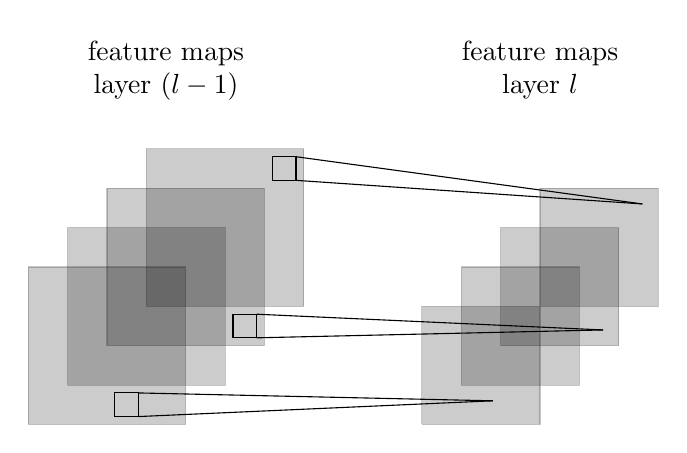
\begin{tikzpicture}
		\node at (1.75,4.5){\begin{tabular}{c}feature maps\\layer $(l-1)$\end{tabular}};
		
		\draw[fill=black,opacity=0.2,draw=black] (1.5,1.5) -- (3.5,1.5) -- (3.5,3.5) -- (1.5,3.5) -- (1.5,1.5);
		\draw[fill=black,opacity=0.2,draw=black] (1,1) -- (3,1) -- (3,3) -- (1,3) -- (1,1);
		\draw[fill=black,opacity=0.2,draw=black] (0.5,0.5) -- (2.5,0.5) -- (2.5,2.5) -- (0.5,2.5) -- (0.5,0.5);
		\draw[fill=black,opacity=0.2,draw=black] (0,0) -- (2,0) -- (2,2) -- (0,2) -- (0,0);
		
		\draw (3.1,3.1) -- (3.4,3.1) -- (3.4,3.4) -- (3.1,3.4) -- (3.1,3.1);
		\draw (2.6,1.1) -- (2.9,1.1) -- (2.9,1.4) -- (2.6,1.4) -- (2.6,1.1);
		\draw (1.1,0.1) -- (1.4,0.1) -- (1.4,0.4) -- (1.1,0.4) -- (1.1,0.1);
		
		\draw (3.4,3.4) -- (7.8,2.8);
		\draw (3.4,3.1) -- (7.8,2.8);
		
		\draw (2.9,1.4) -- (7.3,1.2);
		\draw (2.9,1.1) -- (7.3,1.2);
		
		\draw (1.4,0.4) -- (5.9,0.3);
		\draw (1.4,0.1) -- (5.9,0.3);
		
		\node at (6.5,4.5){\begin{tabular}{c}feature maps\\layer $l$\end{tabular}};
		
		\draw[fill=black,opacity=0.2,draw=black] (6.5,1.5) -- (8,1.5) -- (8,3) -- (6.5,3) -- (6.5,1.5);
		\draw[fill=black,opacity=0.2,draw=black] (6,1) -- (7.5,1) -- (7.5,2.5) -- (6,2.5) -- (6,1);
		\draw[fill=black,opacity=0.2,draw=black] (5.5,0.5) -- (7,0.5) -- (7,2) -- (5.5,2) -- (5.5,0.5);
		\draw[fill=black,opacity=0.2,draw=black] (5,0) -- (6.5,0) -- (6.5,1.5) -- (5,1.5) -- (5,0);
	\end{tikzpicture}
	\caption[Illustration of a pooling layer]{Illustration of a pooling layer. Layer $l$ summarizes the information in layer $l-1$ through some statistical feature (maximum, average, etc). This is accomplished by defining a fixed size window and then scanning the previous layer, applying the pooling operation at each step. The number of feature maps remains the same. Source: \url{https://davidstutz.de/illustrating-convolutional-neural-networks-in-latex-with-tikz/} \cite{conv-graphs}.}
	\label{fig:maxpool}
    \end{figure}
    
    \item \textbf{Fully connected layer:} A feed forward network is used to produce the final output. Since the convolutional and pooling layers already have done the work of extracting relevant spatial features, the fully connected layers can then receive the transformed data.
\end{itemize} 

Furthermore, CNN have properties that benefit their application \cite{cnn-survey}:
\begin{itemize}
    \item \textbf{Sparse interactions:} The number of parameters is reduced compared to fully connected layers since kernels are usually much smaller than the input and this is more efficient in terms of memory usage.
    \item \textbf{Shared weights:} Weights are used multiple times in the model because kernels slide through the input while dense layers have each weight associated with only one feature.
    \item \textbf{Equivariance to translation:} The representation of the input's features is equivariant to the location of features, that is, if the input is translated, the feature maps in each layer will be translated in the same way \cite{dl-book}.
\end{itemize}

\section{Segmentation models}
An important problem in computer vision is the analysis of images or videos for segmentation and it has been addressed using different techniques, including deep learning models which are discussed in this section.

First, the segmentation task encompasses several different but related problems. The most common are: 
\begin{itemize}
    \item \textbf{Object localization:} An image with different subjects is processed and the model is expected to localize them, this is usually done using bounding boxes around every subject.
    
    \item \textbf{Semantic segmentation:} In this case, each pixel of the image is labeled as a subject, so the specific geometry is recognized as opposed to the bounding box localization.
    
    \item \textbf{Instance segmentation:} This expands the semantic segmentation by assigning labels to each instance of a subject within an image. This allows to separate subjects that would have the same label in semantic segmentation.
\end{itemize}

In figure \ref{fig:segment-types} the different types of segmentation are depicted. This thesis is concerned with the application of supervised semantic segmentation models, so the models studied aim to solve that task.

\begin{figure}
  \begin{subfigure}[b]{0.45\textwidth}
    \includegraphics[width=\linewidth]{Images/Background/s1.png}
    \caption{Input image}
    \label{fig:input_img}
  \end{subfigure}
\hfill
  \begin{subfigure}[b]{0.45\textwidth}
    \includegraphics[width=\linewidth]{Images/Background/s2.png}
    \caption{Localization}
    \label{fig:localization}
  \end{subfigure}
  \begin{subfigure}[b]{0.45\textwidth}
    \includegraphics[width=\linewidth]{Images/Background/s3.png}
    \caption{Semantic segmentation}
    \label{fig:semantic}
  \end{subfigure}
\hfill
  \begin{subfigure}[b]{0.45\textwidth}
    \includegraphics[width=\linewidth]{Images/Background/s4.png}
    \caption{Instance segmentation}
    \label{fig:instance}
  \end{subfigure}
  \caption[Typical segmentation tasks]{Typical segmentation tasks. Source: \textit{A survey on deep learning techniques for image and video semantic segmentation} \cite{segmentation-survey-2}.}
  \label{fig:segment-types}
\end{figure}

\subsection{Fully convolutional networks}

Fully Convolutional Networks (FCN) are ANN that only make use of convolutional and pooling layers. This type of architecture is suitable for semantic segmentation because it is possible to have a grid-like output, as opposed to a single value or array of values when fully connected layers are used in the output layer. As stated before, in semantic segmentation it is necessary to assign a label to each pixel in an image to generate groups of pixels that have some semantic or spatial relationship.

A generic FCN architecture is shown in figure \ref{fig:fcn}. The structure is composed of a contracting convolutional path in which subsequent convolutional and pooling layers are applied so the number of feature maps increases (depth) and the size of the input decreases (width and height). Then there is an expanding path in which transposed convolutions\footnote{The term “deconvolution” is sometimes used, but this is discouraged because a deconvolution is defined as the inverse of a convolution, which is different from a transposed convolution \cite{trans-conv}.} are applied and followed by regular convolutions that reduce the number of feature maps. The purpose of transposed convolutions is to upsample the feature maps so the original input shape is recovered. The output is the segmentation map which is an image of the same shape as the input and each pixel has a specific label. In a supervised approach, these labels come from whatever labels have been assigned to the training examples. 

\begin{figure}
	\centering
	\noindent\resizebox{\textwidth}{!}{
	\input{Graphs/fcn}
	}
	\caption[Illustration of a fully convolutional network]{Illustration of a FCN. First, subsequent convolution and pooling layers are applied. In the convolutions the feature maps are added (more length in the figure) while maintaining height and width, then the pooling layer reduces the size while keeping the same number of feature maps. In the expanding path, a transposed convolution is applied which upsamples the feature maps, then a normal convolution is applied reducing the number of feature maps. Source: Adapted from \url{https://github.com/jettan/tikz_cnn}.}
	\label{fig:fcn}
\end{figure}

The main feature of a FCN is the upsampling layer in which the transposed convolution is applied, because without such an operation, it would no be possible to recover the shape of the input. This could be solved by not using pooling layers and maintaining the shape throughout the network, but this would be computationally expensive because the number of parameters would be really large, and one of the benefits of CNN is the possibility to reduce the number of parameters by using small filters compared to the input size.

\subsection{Transposed convolution}
The transposed convolution operation functions in the opposite way of a pooling layer, thus upsampling the input. For this, a kernel with trainable parameters is used. Note that since this is not the inverse of a convolution, the result is just a new collection of feature maps that recovers the shape of the previous layer, but does not have the same parameter values.

As an example, let us consider the convolution shown in figure \ref{fig:no_padding_no_strides}. If we write the convolution as a vector-matrix multiplication, the kernel can be written as
\setcounter{MaxMatrixCols}{20}
\begin{align*}
\resizebox{.98\hsize}{!}{$
   \mathbf{C} =\begin{pmatrix}
    w_{0,0} & w_{0,1} & w_{0,2} & 0       & w_{1,0} & w_{1,1} & w_{1,2} & 0       &
    w_{2,0} & w_{2,1} & w_{2,2} & 0       & 0       & 0       & 0       & 0       \\
    0       & w_{0,0} & w_{0,1} & w_{0,2} & 0       & w_{1,0} & w_{1,1} & w_{1,2} &
    0       & w_{2,0} & w_{2,1} & w_{2,2} & 0       & 0       & 0       & 0       \\
    0       & 0       & 0       & 0       & w_{0,0} & w_{0,1} & w_{0,2} & 0       &
    w_{1,0} & w_{1,1} & w_{1,2} & 0       & w_{2,0} & w_{2,1} & w_{2,2} & 0       \\
    0       & 0       & 0       & 0       & 0       & w_{0,0} & w_{0,1} & w_{0,2} &
    0       & w_{1,0} & w_{1,1} & w_{1,2} & 0       & w_{2,0} & w_{2,1} & w_{2,2} \\
    \end{pmatrix}$}
\end{align*}
where $w_{ij}$ is the weight of the kernel located in row $i$ and column $j$. Then, the convolution can be computed by flattening the input so that it becomes a $16-$dimensional vector. The result is going to be a $4-$dimensional vector which can be reshaped to $2\times2$ to get the matrix form. With this in mind, notice that in the forward pass, the convolution consists in multiplying by $\mathbf{C}$ while in the backward pass to propagate the error it is necessary to multiply by $\mathbf{C}^T$. Hence, the weight matrix defines both the forward and backward pass of the network.

Now consider the idea behind transposed convolution which is to take a small matrix, applying a transformation and obtaining a larger matrix maintaining the number of feature maps. This is precisely what happens when in the backward pass $\mathbf{C}^T$ is applied. Then, multiplying by $\mathbf{C}^T$ is a transposed convolution by definition if $\mathbf{C}^T$ is applied in the forward pass instead of the backward pass.

In general, the process can be thought of as having an input matrix in which every data point is multiplied by the kernel and then summed over the corresponding values. This is equivalent\footnote{This is useful as a concept, but is not used when programming because many of the operations are useless zero multiplications.} to a regular convolution over a fully padded input\footnote{This means the input is padded such that the kernel can overlap its last value (bottom-right) with the first of the input (top-left).} as shown in figure \ref{fig:no_padding_no_strides_transposed} which is a $2\times 2$ input in which a transposed convolution is applied with a $3\times 3$ kernel to produce a $4\times 4$ output or equivalently, a $6 \times 6$ (padded) input convolved with a $3\times 3$ kernel.

\begin{figure}
    \centering
    \includegraphics[width=0.24\textwidth]{Images/Background/Convolution/no_padding_no_strides_transposed_00.pdf}
    \includegraphics[width=0.24\textwidth]{Images/Background/Convolution/no_padding_no_strides_transposed_01.pdf}
    \includegraphics[width=0.24\textwidth]{Images/Background/Convolution/no_padding_no_strides_transposed_02.pdf}
    \includegraphics[width=0.24\textwidth]{Images/Background/Convolution/no_padding_no_strides_transposed_03.pdf}
    \caption[Example of a transposed convolution]{Transposed convolution of a $2\times 2$ input with a $3\times 3$ kernel to produce a $4\times 4$ output. This is equivalent to a regular convolution of a $6\times 6$ input with a $2\times 2$ padding with the same kernel. Source: \url{https://github.com/vdumoulin/conv_arithmetic} \cite{trans-conv}.}
    \label{fig:no_padding_no_strides_transposed}
\end{figure}

\subsection{Residual connections}

As of now, the networks discussed have all been connected using adjacent layers which means every node in one layer is connected with every node in the next layer, no connections are missing and no connections with other layers are added. Nonetheless, a trick that has proven to be very effective when training ANN is the use of residual connections, allowing to achieve state of the art results in a wide range of tasks. These connections consist in having a connection with deeper layers of the network, so a neuron $n$ in layer $l$ can be connected with layer $l+1$ as usual and with other layers $l+r$, $r\geq 1$.

Before residual connections were developed, some deep networks performed worse than shallow ones despite the fact that in theory neural networks are universal approximators \cite{Hornik, Cybenko}, which means that it is possible to approximate any function in a compact domain with an arbitrary small error given enough neural units. Particularly, there was a saturation in accuracy, that is the accuracy improved with depth up to a certain point at which accuracy began to decrease. This is called the degradation problem \cite{res-connection}.

Specifically when a shallow network performs better than a deep one, an intuitive approach would be to allow the deep network to skip some layers so that it can mimic the behavior of a shallow network if needed. Then, if a layer activation is small, an identity mapping can be added so that the gradient does not vanish and the network can make use of that layer's level of abstraction. In figure \ref{fig:res-connection} a residual connection is shown. 

\begin{figure}
    \centering
    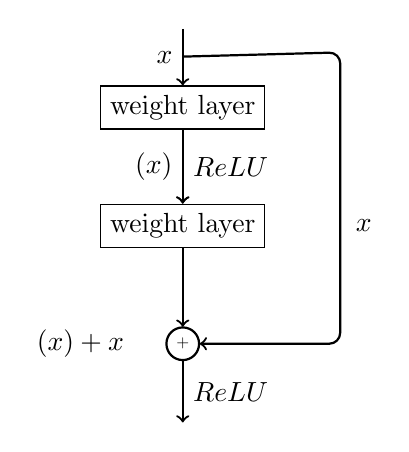
\begin{tikzpicture}
    
    \node[rectangle, draw] (n1) at (0,0) {weight layer};
    \node[rectangle, draw] (n2) at (0,-1.5) {weight layer};
    \node[circle, draw, scale =.6, thick] (n3) at (0,-3) {$\mathbf{+}$};
    
    \draw[thick, ->] (0,1) -- (n1) node[midway, left] (a1) {$x$};
    \draw[thick, ->] (n1) -- (n2) node[midway, left] {$\F (x)$} node[midway, right] {$ReLU$};
    \draw[thick, ->] (n2) -- (n3);
    
    \draw[thick, ->,rounded corners] (a1) -- node[]{} (2,.7) |- (n3);

    \draw[thick, ->] (n3) -- (0,-4) node[midway, right] {$ReLU$};
    
    \draw (-1.3,-3) node[] {$\F(x) + x$};
    \draw (2.3,-1.5) node[] {$x$};
    \draw[thick,->] (n1) -- (n2);
\end{tikzpicture}
    \caption[Residual connection diagram]{Residual connection diagram. Source: Adapted from \textit{Deep residual learning for image recognition} \cite{res-connection}.}
    \label{fig:res-connection}
\end{figure}

In the context of FCN, these residual connections are called \textit{skip layers}, which also skip connections to further layers in the network, but do so by concatenating layers as opposed to the sum shown in \ref{fig:res-connection}. On a semantic level, what the network does when convolving and pooling is extracting more high-level representations of the input. Then, what the skip layers do is recover the layers' low-level information which is the context needed to reconstruct when upsampling \cite{Ronneberger}.
\chapter{Proposed approach using Fully Convolutional Networks}\label{chap:proposed_model}

In this chapter the proposed models are described. These consist in FCN based deep learning architectures which are compared in the same datasets to ensure validated results and also to choose the best performing model for further analysis. The architectures are described using baseline parameters that will then be optimized using a grid search. In figure \ref{fig:flowchart} a flowchart of the proposed framework is shown.

\section{Segmentation architectures}
The architectures used are FCN based, so they share they building blocks shown in figure \ref{fig:fcn}. There is a contracting path of successive convolution and pooling layers and then an expanding path that mirrors the shape of the contracting one by applying transposed convolutions (upsampling) instead of pooling. Also, in the contracting path the number of feature maps increases while in the expanding path it decreases until reaching the output's number of channels. The segmentation architectures used are:

\begin{itemize}
    \item \textbf{DeconvNet:} This network is an FCN which uses a VGGNet \cite{vggnet} as a backbone for the contracting path. The expanding path mirrors the VGGNet architecture. Since it is based in a network that has already proven to have good results with image data it is appropriate to extend its application \cite{vggnet, Noh}. In figure \ref{fig:deconv} the contracting path is shown.

    \item \textbf{U-Net:} The U-Net is an FCN that was first implemented in the biomedical field for microscopy images. The architecture is shown in figure \ref{fig:unet} and makes use of skip layers which are taken from the contracting path and then concatenated in the expanding path layers. This allows the network to localize specific data by reducing dimensionality and also have the context of the general image through the skip layers \cite{Ronneberger}.
    


    \item \textbf{MultiResUnet:} This is an improvement of the U-Net, than can process subjects which have large differences in scale within an image. This is done with several convolutions with different kernels so that the features are learned at different resolutions, this is borrowed from Inception architectures such as GoogLeNet \cite{inception}. The structure is the same as in figure \ref{fig:unet} but the convolution blocks are changed with residual blocks that apply different convolutions which are then summed. Also, skip connections have a residual residual path in between. Figure \ref{fig:multires} shows the residual block used and figure \ref{fig:respath} depicts the residual connections used in the skip layers.
\end{itemize}

\begin{figure}
    \centering
     \resizebox{\linewidth}{!}{
    \includegraphics{Images/Background/framework_flow_chart.pdf}
    }
    \caption[Proposed framework flowchart]{Proposed framework flowchart.}
    \label{fig:flowchart}
\end{figure}

\begin{figure}
    \centering
    \resizebox{\linewidth}{!}{
    \begin{tikzpicture}
\tikzstyle{connection}=[ultra thick,every node/.style={sloped,allow upside down},draw=\edgecolor,opacity=0.7]
\tikzstyle{copyconnection}=[ultra thick,every node/.style={sloped,allow upside down},draw={rgb:blue,4;red,1;green,1;black,3},opacity=0.7]

%%%%%%%%%%%%%%%%%%%%%%%%%%%%%%%%%%%%%%%%%%%%%%%%%%%%%%%%%%%%%%%%%%%%%%%%%%%%%%%%%%%%%%%%
%% Draw Encoder
%%%%%%%%%%%%%%%%%%%%%%%%%%%%%%%%%%%%%%%%%%%%%%%%%%%%%%%%%%%%%%%%%%%%%%%%%%%%%%%%%%%%%%%%
% conv1_1,conv1_2
\pic[shift={(0,0,0)}] at (0,0,0) {RightBandedBox={name=cr1,%
        xlabel={{"64","64"}},ylabel=$3\times3$,zlabel=I,fill=\ConvColor,bandfill=\ConvReluColor,%
        height=40,width={2,2},depth=40}};
%pool1
\pic[shift={(0,0,0)}] at (cr1-east) {Box={name=p1,%
        fill=\PoolColor,opacity=0.5,height=32,width=1,depth=32,ylabel=$2\times2$}};
%%%%%%%%%%
% conv2_1,conv2_2
\pic[shift={(1,0,0)}] at (p1-east) {RightBandedBox={name=cr2,%
        xlabel={{"128","128"}},ylabel=$3\times3$,zlabel=I/2,fill=\ConvColor,bandfill=\ConvReluColor,%
        height=32,width={3.5,3.5},depth=32}};
%pool2
\pic[shift={(0,0,0)}] at (cr2-east) {Box={name=p2,%
        fill=\PoolColor,opacity=0.5,height=25,width=1,depth=25,ylabel=$2\times2$}};
%%%%%%%%%%
% conv3_1,conv3_2
\pic[shift={(0.75,0,0)}] at (p2-east) {RightBandedBox={name=cr3,%
        xlabel={{"256","256","256"}},ylabel=$3\times3$,zlabel=I/4,fill=\ConvColor,bandfill=\ConvReluColor,%
        height=25,width={4.5,4.5,4.5},depth=25}};
%pool3
\pic[shift={(0,0,0)}] at (cr3-east) {Box={name=p3,%
        fill=\PoolColor,opacity=0.5,height=16,width=1,depth=16,ylabel=$2\times2$}};
%%%%%%%%%%
% conv4_1,conv4_2,conv4_3
\pic[shift={(0.5,0,0)}] at (p3-east) {RightBandedBox={name=cr4,%
        xlabel={{"512","512","512"}},ylabel=$3\times3$,zlabel=I/8,fill=\ConvColor,bandfill=\ConvReluColor,%
        height=16,width={6,6,6},depth=16}};
%pool4
\pic[shift={(0,0,0)}] at (cr4-east) {Box={name=p4,%
        fill=\PoolColor,opacity=0.5,height=8,width=1,depth=8,ylabel=$2\times2$}};
%%%%%%%%%%%%%%%%%%%%%%%%%%%%%%%%%%%%%%%%%%%%%%%%%%%%%%%%%%%%%%%%%%%%%%%%%%%%%%%%%%%%%%%%
%% Bottleneck
%%%%%%%%%%%%%%%%%%%%%%%%%%%%%%%%%%%%%%%%%%%%%%%%%%%%%%%%%%%%%%%%%%%%%%%%%%%%%%%%%%%%%%%%% conv5_1,conv5_2,conv5_3
\pic[shift={(0.75,0,0)}] at (p4-east) {RightBandedBox={name=cr5,%
        xlabel={{"512","512","512"}},ylabel=$3\times3$,zlabel=I/16,fill=\ConvColor,bandfill=\ConvReluColor,%
        height=8,width={6,6,6},depth=8}};

%pool5
\pic[shift={(0,0,0)}] at (cr5-east) {Box={name=p5,%
        fill=\PoolColor,opacity=0.5,height=5,width=.7,depth=5,ylabel=$7\times7$}};
        
\pic[shift={(1,0,0)}] at (cr5-east) {RightBandedBox={name=fc,%
        xlabel={{"4096","4096"}},zlabel=I/32,fill=\ConvColor,bandfill=\ConvReluColor,%
        height=2,width={12,12},depth=2}};
%%%%%%%%%%%%%%%%%%%%%%%%%%%%%%%%%%%%%%%%%%%%%%%%%%%%%%%%%%%%%%%%%%%%%%%%%%%%%%%%%%%%%%%%
%% Draw Decoder 
%%%%%%%%%%%%%%%%%%%%%%%%%%%%%%%%%%%%%%%%%%%%%%%%%%%%%%%%%%%%%%%%%%%%%%%%%%%%%%%%%%%%%%%%

%%%%%%%%%%%%%%%%%%%%%%%%%%%%%%%%%%%%%%%%%%%%%%%%%%%%%%%%%%%%%%%%%%%%%%%%%%%%%%%%%%%%%%%
% Draw connections
%%%%%%%%%%%%%%%%%%%%%%%%%%%%%%%%%%%%%%%%%%%%%%%%%%%%%%%%%%%%%%%%%%%%%%%%%%%%%%%%%%%%%%%
\draw [connection]  (p1-east)    -- node {\midarrow} (cr2-west);
\draw [connection]  (p2-east)    -- node {\midarrow} (cr3-west);
\draw [connection]  (p3-east)    -- node {\midarrow} (cr4-west);
\draw [connection]  (p4-east)    -- node {\midarrow} (cr5-west);
\draw [connection]  (p5-east)    -- node {\midarrow} (fc-west);


%%%%%%%%%%%%%%%%%%%%%%%%%%%%%%%%%%%%%%%%%%%%%%%%%%%%%%%%%%%%%%%%%%%%%%%%%%%%%%%%%%%%%%%
\end{tikzpicture}
    }
    \caption[Illustration of a DeconvNet contracting path]{Illustration of a DeconvNet contracting path. A VGGNet architecture is used and then mirrored in the expanding path. At the top of each block the kernel shape is shown, below are depicted the number of feature maps per convolution. Finally, $I$ is the input size which is halved after each pooling layer. Source: Adapted from \url{https://github.com/HarisIqbal88/PlotNeuralNet}.}
    \label{fig:deconv}
\end{figure}

\begin{figure}
    \centering
    \resizebox{\linewidth}{!}{
    \input{Graphs/unet}
    }
    \caption[Illustration of a U-Net architecture]{Illustration of a U-Net architecture. The architecture is divided in a contracting path and an expanding path. The contracting path has conv (yellow)/conv/pool (red) blocks. The expanding path has transposed-conv (blue)/conv/conv blocks. Dimensions in the expanding path mirror the contracting path. Each convolution before pooling is used as a skip layer and concatenated with the corresponding shape in the expanding path. The final layer reduces the feature maps to one and applies a softmax function for pixel-wise classification. Convolution kernels are $3\times 3$ while pooling kernels are $2\times 2$ so the size is halved at each block. Source: Adapted from \url{https://github.com/HarisIqbal88/PlotNeuralNet}.}
    \label{fig:unet}
\end{figure}

\begin{figure}
    \centering
    \resizebox{\linewidth}{!}{
    \begin{tikzpicture}
\tikzstyle{connection}=[ultra thick,every node/.style={sloped,allow upside down},draw=\edgecolor,opacity=0.7]
\tikzstyle{copyconnection}=[ultra thick,every node/.style={sloped,allow upside down},draw={rgb:blue,4;red,1;green,1;black,3},opacity=0.7]

%%%%%%%%%%%%%%%%%%%%%%%%%%%%%%%%%%%%%%%%%%%%%%%%%%%%%%%%%%%%%%%%%%%%%%%%%%%%%%%%%%%%%%%%
%% Draw Encoder
%%%%%%%%%%%%%%%%%%%%%%%%%%%%%%%%%%%%%%%%%%%%%%%%%%%%%%%%%%%%%%%%%%%%%%%%%%%%%%%%%%%%%%%%
% conv1_1,conv1_2
\def\ConvColor{rgb:red,50;green,227;blue,150}
\def\ConvReluColor{rgb:red,50;green,200;blue,100}

\pic[shift={(0,0,0)}] at (0,0,0) {RightBandedBox={name=cr1,ylabel=$3\times3$,fill=\ConvColor,bandfill=\ConvReluColor,%
        height=20,width={0.5},depth=20}};

\node[inner sep=0,minimum size=0] (o0) at (-2,0,0) {}; % invisible node

\node[inner sep=0,minimum size=0,right of=o0] (k0) {}; % invisible node

\node[inner sep=0,minimum size=0] (o1) at (0,0,0) {}; % invisible node

\node[inner sep=0,minimum size=0,right of=o1] (k1) {}; % invisible node

\node[inner sep=0,minimum size=0] (o2) at (2.3,0,0) {}; % invisible node

\node[inner sep=0,minimum size=0,right of=o2] (k2) {}; % invisible node

%%%%%%%%%%
% conv2_1,conv2_2
\pic[shift={(2,0,0)}] at (cr1-east) {RightBandedBox={name=cr2,%
        xlabel={{"",""}},ylabel=$3\times3$,fill=\ConvColor,bandfill=\ConvReluColor,%
        height=20,width={0.5,0.5},depth=20}};
%%%%%%%%%%
% conv3_1,conv3_2
\pic[shift={(2,0,0)}] at (cr2-east) {RightBandedBox={name=cr3,ylabel=$3\times3$,fill=\ConvColor,bandfill=\ConvReluColor,%
        height=20,width={0.5,0.5,0.5,0.5},depth=20}};

        
%%%%%%%%%%
% conv4_1,conv4_2,conv4_3
\pic[shift={(2,0,0)}] at (cr3-east) {RightBandedBox={name=cr4,ylabel=\hspace{-5pt}Concatenation,fill=\ConvColor,bandfill=\ConvReluColor,%
        height=10,width={3,3,3},depth=10}};

%%%%%%%%%%
% conv3_1,conv3_2
\pic[shift={(0,5,0)}] at (cr3-east) {RightBandedBox={name=id,ylabel=$1\times1$,fill=blue!20,bandfill=blue!20,%
        height=10,width={0.5},depth=10}};


\node[draw,circle,minimum size=1.6cm,inner sep=0pt, color = black, very thick, fill = black!5] (sum) at (12,0) {\Huge $\mathbf{+}$};

\node[inner sep=0,minimum size=0] (k3) at (15,0) {}; % invisible node
%%%%%%%%%%%%%%%%%%%%%%%%%%%%%%%%%%%%%%%%%%%%%%%%%%%%%%%%%%%%%%%%%%%%%%%%%%%%%%%%%%%%%%
% Draw connections
%%%%%%%%%%%%%%%%%%%%%%%%%%%%%%%%%%%%%%%%%%%%%%%%%%%%%%%%%%%%%%%%%%%%%%%%%%%%%%%%%%%%%%%
\draw node (I) at (-3,0,0) {Input};

\draw [connection]  (I)    -- node {\midarrow} (cr1-west);
\draw [connection]  (cr1-east)    -- node {\midarrow} (cr2-west);
\draw [connection]  (cr1-east)    -- node {\midarrow} (cr2-west);
\draw [connection]  (cr2-east)    -- node {\midarrow} (cr3-west);
\draw [connection]  (cr3-east)    -- node {\midarrow} (cr4-west);
\draw [connection]  (cr4-east)    -- node {\midarrow} (sum);
\draw [connection]  (sum)    -- node {\midarrow} (k3);



\draw [connection]  (k1) - ++(0,-4) -| node {\midarrow} (cr4-southeast);
\draw [connection]  (k2) - ++(0,-3) -| node {\midarrow} (cr4-south);
\draw [connection]  (k0) |- node {\midarrow} (id-west);
\draw [connection]  (id-east) -| node {\midarrow} (sum);




%%%%%%%%%%%%%%%%%%%%%%%%%%%%%%%%%%%%%%%%%%%%%%%%%%%%%%%%%%%%%%%%%%%%%%%%%%%%%%%%%%%%%%%
\end{tikzpicture}

    }
    \caption[Illustration of a Multi Resolution block]{Illustration of a Multi Resolution block. The block consists of successive convolutions which are then stacked via skip layers and then summed using a residual connection. The second and third convolutional blocks are stacked convolutions of $3\times3$ kernels which are factorized operations of $5\times 5$ and $7 \times7$ convolutions respectively \cite{conv-factor}. This approach is more computationally efficient than using parallel higher resolution kernels. Source: Adapted from \url{https://github.com/HarisIqbal88/PlotNeuralNet}.}
    \label{fig:multires}
\end{figure}

\begin{figure}
    \centering
    \resizebox{0.5\linewidth}{!}{
    \begin{tikzpicture}
\tikzstyle{connection}=[ultra thick,every node/.style={sloped,allow upside down},draw=\edgecolor,opacity=0.7]
\tikzstyle{copyconnection}=[ultra thick,every node/.style={sloped,allow upside down},draw={rgb:blue,4;red,1;green,1;black,3},opacity=0.7]

%%%%%%%%%%%%%%%%%%%%%%%%%%%%%%%%%%%%%%%%%%%%%%%%%%%%%%%%%%%%%%%%%%%%%%%%%%%%%%%%%%%%%%%%
%% Draw Encoder
%%%%%%%%%%%%%%%%%%%%%%%%%%%%%%%%%%%%%%%%%%%%%%%%%%%%%%%%%%%%%%%%%%%%%%%%%%%%%%%%%%%%%%%%
% conv1_1,conv1_2
\def\ConvColor{rgb:red,50;green,227;blue,150}
\def\ConvReluColor{rgb:red,50;green,200;blue,100}

\pic[shift={(0,0,0)}] at (0,0,0) {RightBandedBox={name=cr1,ylabel=$3\times3$,fill=\ConvColor,bandfill=\ConvReluColor,%
        height=15,width={0.5},depth=15}};

\node[inner sep=0,minimum size=0] (o0) at (-2,0,0) {}; % invisible node

\node[inner sep=0,minimum size=0,right of=o0] (k0) {}; % invisible node


%%%%%%%%%%
% conv3_1,conv3_2
\pic[shift={(2,4,0)}] at (cr1-east) {RightBandedBox={name=id,ylabel=$1\times1$,fill=blue!20,bandfill=blue!20,%
        height=10,width={0.5},depth=10}};


\node[draw,circle,minimum size=1cm,inner sep=0pt, color = black, very thick, fill = black!5] (sum) at (5,0) {\Huge $\mathbf{+}$};

\node[inner sep=0,minimum size=0] (k3) at (7,0) {}; % invisible node
%%%%%%%%%%%%%%%%%%%%%%%%%%%%%%%%%%%%%%%%%%%%%%%%%%%%%%%%%%%%%%%%%%%%%%%%%%%%%%%%%%%%%%
% Draw connections
%%%%%%%%%%%%%%%%%%%%%%%%%%%%%%%%%%%%%%%%%%%%%%%%%%%%%%%%%%%%%%%%%%%%%%%%%%%%%%%%%%%%%%%
\draw node (I) at (-3,0,0) {Input};

\draw [connection]  (I)    -- node {\midarrow} (cr1-west);
\draw [connection]  (cr1-east)    -- node {\midarrow} (sum);
\draw [connection]  (sum)    -- node {\midarrow} (k3);

\draw [connection]  (k0) |- node {\midarrow} (id-west);
\draw [connection]  (id-east) -| node {\midarrow} (sum);




%%%%%%%%%%%%%%%%%%%%%%%%%%%%%%%%%%%%%%%%%%%%%%%%%%%%%%%%%%%%%%%%%%%%%%%%%%%%%%%%%%%%%%%
\end{tikzpicture}
    }
    \caption[Illustration of a residual path]{Illustration of a residual path. This type of block is used in series in the MultiResUnet in between skip layers, so the skipped features are processed before being concatenated to the expanding path. Source: Adapted from \url{https://github.com/HarisIqbal88/PlotNeuralNet}.}
    \label{fig:respath}
\end{figure}

\clearpage
\section{Segmentation loss function}

As stated earlier, to train a supervised neural network it is necessary to have some measure of error so that it can be minimized with respect to the weights. This measure is the loss function which depends on the task. In the case of semantic segmentation, it is necessary to use a loss function that can capture pixel-wise comparisons. Specifically, for supervised segmentation, the input is an image, the output is a 2D mapping of each pixel of the image to a certain class (e.g. pixel$ = 0$ if background and pixel$ = 1$ if foreground) and the output is compared through the loss function with a previously labeled image with the same kind of segmentation mapping corresponding to the input image. A widely used loss metric for supervised semantic segmentation is the intersection over union metric, also known as Jaccard index. This metric is given by
\begin{align*}
    J(A, B) = \frac{|A\cap B|}{|A\cup B|}
\end{align*}
where $|\cdot|$ is the cardinality of the set. Hence, if the overlap is perfect $|A\cap B|=|A\cup B|\xrightarrow[]{} J=1$. Conversely, if there is no overlap $|A\cap B|=0\xrightarrow{} J=0$. In a segmentation mapping, $|A\cap B|$ can be computed as the element-wise multiplication of $A$ and $B$, and then sum the result. Furthermore, $|\cdot|$ is computed as the sum of the matrix' elements. The score is computed over all classes and then averaged.
    
In order to minimize a loss function using the Jaccard index, the Jaccard distance is defined and is given by
\begin{align*}
    d_j(A,B)=1-J(A,B)
\end{align*}

\section{Validation}
The proposed architectures have to be validated to ensure that the best results are obtained. Then, every model is subject to a grid search. The parameters used for grid search are shown in table \ref{table:grid_search}. Also, each model (i.e. each point in the grid) is run using $k$-fold cross validation with $k=4$. That is, each model is run four times with a different and disjoint $25\%$ of validation data each time. The average loss in the validation set is used to compare the models' performances and choose the best one. The parameters are considered for each proposed architecture. Also, separate models are trained for globular and spray datasets.

\begin{table}
\centering
\caption{Hyperparameters used for grid search. Every parameter is used for each proposed architecture (DeconvNet, U-Net and MultiResUnet) and each dataset (globular and spray) is trained separately.}
\label{table:grid_search}
\begin{tabular}{|c|c|c|c|c|}
\cline{1-2} \cline{4-5}
Batch size                                              & 8, 16, 32       &  & Epochs        & \begin{tabular}[c]{@{}c@{}}Max: 200\\ Patience: 20\end{tabular} \\ \cline{1-2} \cline{4-5} 
Filters                                                 & 8, 16, 32       &  & Loss function & \begin{tabular}[c]{@{}c@{}}Jaccard\\ distance\end{tabular}      \\ \cline{1-2} \cline{4-5} 
\begin{tabular}[c]{@{}c@{}}Learning\\ rate\end{tabular} & .01, .005, .001 &  & Optimizer     & Adam                                                            \\ \cline{1-2} \cline{4-5} 
\end{tabular}
\end{table}

\chapter{Dataset}\label{chap:dataset}
In the following chapter the case studies considered in this thesis is detailed, specifically the datasets used and the preprocessing that later leads to the input of the proposed model.

\section{Video files}
The study case consists in analyzing high speed video data from GMAW processes, namely globular and spray transfer. The videos are raw \texttt{.cine} files which can be inspected using the \textit{Phantom Camera Control} (PCC) software. Since the processes are characterized by their transfer mode, one video for each is used. In tables \ref{table:glob_params} and \ref{table:spray_params} the parameters of each video are shown. 

After inspecting the metadata of the video in PCC, they are read in python using the \textit{pycine} library\footnote{\url{https://github.com/OTTOMATIC-IO/pycine}}. Then, each frame is stored into an \texttt{.npz} file. In figures \ref{fig:glob_samples} and \ref{fig:spray_samples} frames of each transfer mode can be seen, particularly the main characteristic of larger droplets in globular and smaller droplets in spray\footnote{Similar videos found at \url{https://sites.ualberta.ca/~ccwj/videos/pages/Intro\%20High\%20Speed/}}.

Notice that later, to calculate physical properties of the process, there has to be a relationship between the pixel and real distance. This can be done using the wire's diameter, since that is a fixed length that is always visible in the image. Using that relationship, the pixel to distance is

\begin{align*}
    \text{Wire's diameter} &= 0.045\;in = 26\;px = 1.143\;mm\\
    1\;px &= 0.0439615\;mm =4.39615\cdot 10^{-5}\;m
\end{align*}

\begin{table}
\centering
\caption[Globular transfer video parameters]{Globular transfer video parameters.}
\label{table:glob_params}
\begin{tabular}{|l|l|lll}
\cline{1-2} \cline{4-5}
Electrode       & $ER70S-6$             & \multicolumn{1}{l|}{} & \multicolumn{1}{l|}{Shielding gas}     & \multicolumn{1}{l|}{$85\%$ $Ar$, $15\%$ $CO_2$} \\ \cline{1-2} \cline{4-5} 
Size            & $0.045''$ ($1.2$ $mm$)     & \multicolumn{1}{l|}{} & \multicolumn{1}{l|}{Number of frames}  & \multicolumn{1}{l|}{$9947$}              \\ \cline{1-2} \cline{4-5} 
Wire feed speed & $175$ $ipm$ ($4.4$ $m/min$) & \multicolumn{1}{l|}{} & \multicolumn{1}{l|}{Resolution}        & \multicolumn{1}{l|}{$352 \times 296$}           \\ \cline{1-2} \cline{4-5} 
Voltage         & $33$ $V$                 & \multicolumn{1}{l|}{} & \multicolumn{1}{l|}{Frame rate} & \multicolumn{1}{l|}{$3000$}              \\ \cline{1-2} \cline{4-5} 
Travel speed    & $20$ $ipm$ ($0.5$ $m/min$)  & \multicolumn{1}{l|}{} & \multicolumn{1}{l|}{Period}            & \multicolumn{1}{l|}{$333.3$ $\mu s$}           \\ \cline{1-2} \cline{4-5} 
CTWD & $0.7''$ ($18$ $mm$) &\multicolumn{1}{l|}{} & \multicolumn{1}{l|}{File size}            & \multicolumn{1}{l|}{$2.01$ $Gb$}  \\ \cline{1-2}\cline{4-5} 
\end{tabular}
\end{table}

\begin{table}
\centering
\caption[Spray transfer video parameters]{Spray transfer video parameters.}
\label{table:spray_params}
\begin{tabular}{|l|l|lll}
\cline{1-2} \cline{4-5}
Electrode       & $ER70S-6$             & \multicolumn{1}{l|}{} & \multicolumn{1}{l|}{Shielding gas}     & \multicolumn{1}{l|}{$85\%$ $Ar$, $15\%$ $CO_2$} \\ \cline{1-2} \cline{4-5} 
Size            & $0.045''$ ($1.2$ $mm$)     & \multicolumn{1}{l|}{} & \multicolumn{1}{l|}{Number of frames}  & \multicolumn{1}{l|}{$6691$}              \\ \cline{1-2} \cline{4-5} 
Wire feed speed & $400$ $ipm$ ($10$ $m/min$) & \multicolumn{1}{l|}{} & \multicolumn{1}{l|}{Resolution}        & \multicolumn{1}{l|}{$352 \times 352$}           \\ \cline{1-2} \cline{4-5} 
Voltage         & $35$ $V$                 & \multicolumn{1}{l|}{} & \multicolumn{1}{l|}{Frame rate} & \multicolumn{1}{l|}{$3000$}              \\ \cline{1-2} \cline{4-5} 
Travel speed    & $20$ $ipm$ ($0.5$ $m/min$)  & \multicolumn{1}{l|}{} & \multicolumn{1}{l|}{Period}            & \multicolumn{1}{l|}{$333.3$ $\mu s$}           \\ \cline{1-2} \cline{4-5} 
CTWD & $0.7''$ ($18$ $mm$) &\multicolumn{1}{l|}{} & \multicolumn{1}{l|}{File size}            & \multicolumn{1}{l|}{$1.61$ $Gb$}  \\ \cline{1-2}\cline{4-5} 
\end{tabular}
\end{table}




\begin{figure}
    \centering
    \begin{subfigure}[b]{0.3\textwidth}
        \includegraphics[width=\textwidth]{Images/Dataset/glob_sample_0.jpg}
        \caption{}
    \end{subfigure}
\hfill
    \begin{subfigure}[b]{0.3\textwidth}
        \includegraphics[width=\textwidth]{Images/Dataset/glob_sample_749.jpg}
        \caption{}
        \label{fig:glob_sample_irregular}
    \end{subfigure}
\hfill
    \begin{subfigure}[b]{0.3\textwidth}
        \includegraphics[width=\textwidth]{Images/Dataset/glob_sample_1506.jpg}
        \caption{}
    \end{subfigure}

    \caption[Globular transfer mode frames]{Globular transfer mode frames.}
    \label{fig:glob_samples}
\end{figure}

\begin{figure}[htbp]
    \centering
    \begin{subfigure}[b]{0.3\textwidth}
        \includegraphics[width=\linewidth]{Images/Dataset/spray_sample_0.jpg}
        \caption{}
    \end{subfigure}
\hfill
    \begin{subfigure}[b]{0.3\textwidth}
        \includegraphics[width=\linewidth]{Images/Dataset/spray_sample_77.jpg}
        \caption{}
    \end{subfigure}
\hfill
    \begin{subfigure}[b]{0.3\textwidth}
        \includegraphics[width=\linewidth]{Images/Dataset/spray_sample_484.jpg}
        \caption{}
    \end{subfigure}

    \caption[Spray transfer mode frames]{Spray transfer mode frames.}
    \label{fig:spray_samples}
\end{figure}

\section{Labeling}
In order to train a supervised deep learning model, manual labels are made using the images as input and masking the droplet. This is done using the LabelBox platform which allows to make such segmentation masks and then download the pairs of input image and corresponding mask. A number of 150 images were segmented for each transfer mode. Some of the resulting masks are shown in figures \ref{fig:glob_sample_masks} and \ref{fig:spray_sample_masks} for globular and transfer respectively.

\begin{figure}[htbp]
    \begin{subfigure}[b]{0.4\textwidth}
        \includegraphics[width=\linewidth]{Images/Dataset/globular_image.jpg}
        \caption{Original frame}
    \end{subfigure}
\hfill
    \begin{subfigure}[b]{0.4\textwidth}
        \includegraphics[width=\linewidth]{Images/Dataset/globular_mask.jpg}
        \caption{Manual segmentation mask}
    \end{subfigure}
    
    \caption[Examples of manually segmented frames for globular transfer]{Examples of manually segmented frames using LabelBox for globular transfer.}
    \label{fig:glob_sample_masks}
\end{figure}

\begin{figure}[htbp]
    \begin{subfigure}[b]{0.4\textwidth}
        \includegraphics[width=\linewidth]{Images/Dataset/spray_image.jpg}
        \caption{Original frame}
    \end{subfigure}
\hfill
    \begin{subfigure}[b]{0.4\textwidth}
        \includegraphics[width=\linewidth]{Images/Dataset/spray_mask.jpg}
        \caption{Manual segmentation mask}
    \end{subfigure}
    
    \caption[Examples of manually segmented frames for spray transfer]{Examples of manually segmented frames using LabelBox for spray transfer.}
    \label{fig:spray_sample_masks}
\end{figure}

The selection of the training images was not random, the images were selected to have as much of the variety of the process as possible, that is the droplet formation, growth and release as well as some deviations such as irregular droplet shape (figure \ref{fig:glob_sample_irregular}, horizontal droplet movement as opposed to vertical, among others. Since most of the frames are from the growth process because it takes more time, it would be counterproductive to choose random frames because one would run into the risk of choosing most, if not all, images from the growth process, inadvertently ignoring the rest.

Notice that although the images have color, it is mostly a gradient from white to black through different intensities of magenta so the images are used as grayscale because the same information can be captured with a third of file size.

\section{Data augmentation}
A total of 150 images were labeled for each transfer mode. Since the number of images is low, data augmentation is used applying flips and rotations of the original labels. Each example is augmented such that it produces 5 different training examples. Therefore, the augmented dataset has 750 images for each transfer mode. In figure \ref{fig:augmented_sample}\footnote{Image \ref{fig:augmented_sample} has different colors compared to images in previous figures, this is due to the color map used when plotting the grayscale image in python. Nonetheless, pixel values are the same.} an example of an augmented input is shown and in table \ref{table:dataset_summary} a summary of the dataset information is shown.

The augmentations were made in python using the library imgaug and are listed as follows: 
\begin{itemize}
    \item Pixel dropout between $0\%$ and $5\%$, which means a probability is sampled uniformly such that $p \in [0, 0.05]$ for each augmented image so that every pixel has a probability $p$ of being turned to zero. In practice, every image will lose random pixels up to a maximum of $5\%$ of the whole image.
    \item Rotations between $-45^\circ$ and $45^\circ$.
    \item Elastic transformations with $\alpha \in [20, 50]$ and $\sigma\in [4,5]$ sampled uniformly from their respective intervals for each augmented image, where $\alpha$ is the strength of the distortion field. Higher values mean that pixels are moved further with respect to the distortion field's direction. $\sigma$ is the standard deviation of the Gaussian kernel used to smooth the distortion  
    fields. This gives the images a ripple effect.
    \item Additive Gaussian noise with mean $\mu=0$ and standard deviation $\sigma\in[0,15]$ sampled uniformly for each augmented image.
\end{itemize}

Notice in figure \ref{fig:augmented_sample} that the sampling of parameters within intervals for each image makes it so that some images are slightly changed while others are more heavily augmented.
\begin{figure}
    \centering
    \import{Images/Dataset/augmented_sample/}{augmented_sample.pgf}
    \caption[Sample of an augmented image and mask]{Sample of an augmented image and respective mask (top left) using pixel dropout, rotation, elastic transformation and additive Gaussian noise.}
    \label{fig:augmented_sample}
\end{figure}


\begin{table}
\centering
\caption[Dataset summary]{Dataset summary per transfer mode.}
\label{table:dataset_summary}

    \begin{tabular}{|c|c|}
        \hline
        \begin{tabular}[c]{@{}c@{}}Manually \\ segmented images\end{tabular} & $150$                                                                          \\ \hline
        Augmented images & $750$           \\ \hline
        Shape                                                                & \begin{tabular}[c]{@{}c@{}}$352\times 288$ (globular)\\ $352\times 352$ (spray)\end{tabular} \\ \hline
        Channels         & $1$ (grayscale) \\ \hline
    \end{tabular}
\end{table}



\chapter{Results and analysis}\label{chap:results}
In this chapter, the results are shown and discussed covering the model selection process, training, testing and post processing. It is worth mentioning that since this thesis is focused on analyzing videos, there is a great value in having video results as well but because of the format, only sampled images can be shown. Nevertheless, in the GitHub project\footnote{\url{https://github.com/igonzalezperez/Welding-droplet-analysis-using-fully-convolutional-networks}.} are all the video results which generate the images shown in this chapter. These are specially useful for analyzing the post processing results.


\section{Grid search}
The three proposed architectures' hyperparameters are optimized through grid search (see table \ref{table:grid_search}). Also, 4-fold cross validation is performed so that every model is run over four different and disjoint combinations of training and validation set. Therefore, every model yields four training loss and validation loss values which can then be averaged and used to compare between models. 

In tables \ref{table:globular_best_models} and \ref{table:spray_best_models} the three best models for each proposed architecture are shown for globular and spray transfer respectively\footnote{All of the results of the grid search are shown in Appendix \ref{appendix_gs}}. The results show that the best model is the U-Net in every case, while the MultiResUnet has the worst performance and the DeconvNet is between the other two, closer to the MultiResUnet. Hence the U-Net architecture seems suitable to solve the task at hand. 

The low performance of the MultiResUnet can be explained by the fact that it is considerably more complex than the alternatives and the problem of droplet detection is relatively simple if compared to other computer vision tasks such as traffic image segmentation in which a wide variety of subjects (in terms of geometry, color, scale, etc.) can be found. Moreover, in table \ref{table:globular_best_models} the first two MultiResUnet models have a low number of epochs, especially considering that the patience is of 20 epochs when applying the early stopping criteria. Then, a higher patience could improve those results but this is not clear since the third best model does have higher number of epochs and performs similarly. Furthermore, the better performance of U-Net over DeconvNet is to be expected, since the U-Net incorporates skip layers while DeconvNet is a vanilla FCN. Also, notice that the standard deviation is always one order of magnitude below the average, which means the individual results do not differ significantly. Hence, the models are robust since they perform similarly across different sets of validation data.

\begin{table}
\centering
\caption[Grid search results for globular dataset]{Grid search results for globular dataset. The best three models for each architecture are shown based on the average validation loss over 4-fold cross validation.}
\label{table:globular_best_models}
\begin{tabular}{llllllllllll}
 &
   &
   &
   &
  \multicolumn{4}{l}{\begin{tabular}[c]{@{}l@{}}Last\\ epoch\end{tabular}} &
  \multicolumn{2}{l}{\begin{tabular}[c]{@{}l@{}}Train\\ loss\end{tabular}} &
  \multicolumn{2}{l}{\begin{tabular}[c]{@{}l@{}}Val.\\ loss\end{tabular}} \\
Architecture &
  \begin{tabular}[c]{@{}l@{}}Batch\\ size\end{tabular} &
  Filters &
  \begin{tabular}[c]{@{}l@{}}Learning\\ rate\end{tabular} &
  1 &
  2 &
  3 &
  4 &
  Mean &
  \begin{tabular}[c]{@{}l@{}}Std.\\ dev.\end{tabular} &
  Mean &
  \begin{tabular}[c]{@{}l@{}}Std.\\ dev.\end{tabular} \\ \hline
U-Net     & 16 & 32 & 0.001 & 95  & 82  & 118 & 67  & 0.1  & 0.015 & 0.19 & 0.028 \\
U-Net     & 32 & 8  & 0.01  & 155 & 95  & 83  & 68  & 0.13 & 0.025 & 0.2  & 0.006 \\
U-Net     & 32 & 8  & 0.001 & 93  & 106 & 82  & 85  & 0.12 & 0.007 & 0.2  & 0.02  \\
DeconvNet & 32 & 8  & 0.001 & 151 & 52  & 75  & 89  & 0.21 & 0.065 & 0.35 & 0.029 \\
DeconvNet & 8  & 16 & 0.001 & 68  & 90  & 89  & 105 & 0.2  & 0.025 & 0.37 & 0.013 \\
DeconvNet & 8  & 8  & 0.001 & 154 & 74  & 94  & 74  & 0.2  & 0.03  & 0.37 & 0.038 \\
MultiRes  & 8  & 8  & 0.01  & 24  & 41  & 46  & 63  & 0.5  & 0.008 & 0.52 & 0.117 \\
MultiRes  & 16 & 16 & 0.01  & 49  & 34  & 41  & 39  & 0.5  & 0.009 & 0.52 & 0.018 \\
MultiRes  & 8  & 32 & 0.001 & 111 & 106 & 94  & 116 & 0.48 & 0.006 & 0.55 & 0.025
\end{tabular}
\end{table}

\begin{table}
\centering
\caption[Grid search results for spray dataset]{Grid search results for spray dataset. The best three models for each architecture are shown based on the average validation loss over 4-fold cross validation.}
\label{table:spray_best_models}
\begin{tabular}{llllllllllll}
\multicolumn{4}{l}{} &
  \multicolumn{4}{l}{\begin{tabular}[c]{@{}l@{}}Last\\ epoch\end{tabular}} &
  \multicolumn{2}{l}{\begin{tabular}[c]{@{}l@{}}Train\\ loss\end{tabular}} &
  \multicolumn{2}{l}{\begin{tabular}[c]{@{}l@{}}Val.\\ loss\end{tabular}} \\
Architecture &
  \begin{tabular}[c]{@{}l@{}}Batch\\ size\end{tabular} &
  Filters &
  \begin{tabular}[c]{@{}l@{}}Learning\\ rate\end{tabular} &
  1 &
  2 &
  3 &
  4 &
  Mean &
  \begin{tabular}[c]{@{}l@{}}Std.\\ dev.\end{tabular} &
  Mean &
  \begin{tabular}[c]{@{}l@{}}Std.\\ dev.\end{tabular} \\ \hline
U-Net     & 8  & 8  & 0.005 & 74  & 91  & 105 & 122 & 0.23 & 0.017 & 0.28 & 0.008 \\
U-Net     & 8  & 8  & 0.001 & 113 & 97  & 74  & 114 & 0.2  & 0.019 & 0.28 & 0.006 \\
U-Net     & 8  & 16 & 0.005 & 144 & 119 & 93  & 111 & 0.19 & 0.01  & 0.28 & 0.009 \\
DeconvNet & 16 & 16 & 0.001 & 85  & 101 & 80  & 69  & 0.27 & 0.013 & 0.45 & 0.008 \\
DeconvNet & 8  & 8  & 0.001 & 63  & 90  & 76  & 80  & 0.32 & 0.021 & 0.47 & 0.016 \\
DeconvNet & 16 & 8  & 0.001 & 76  & 94  & 86  & 105 & 0.27 & 0.024 & 0.47 & 0.018 \\
MultiRes  & 8  & 16 & 0.005 & 94  & 43  & 64  & 47  & 0.35 & 0.013 & 0.43 & 0.021 \\
MultiRes  & 8  & 32 & 0.005 & 76  & 68  & 61  & 75  & 0.32 & 0.007 & 0.43 & 0.038 \\
MultiRes  & 16 & 8  & 0.005 & 53  & 107 & 78  & 100 & 0.34 & 0.017 & 0.45 & 0.049
\end{tabular}
\end{table}

\section{Training}

After the grid search, the best models are selected based on the average validation loss and then these models are saved to make predictions. In figures \ref{fig:globular_loss_curve} and \ref{fig:spray_loss_curve} the learning curves for the globular and spray models are shown respectively. These graphs show that the training is indeed successful, steadily reaching a low loss value both in training and validation. The gap between the two is to be expected and the fact that the two curves show similar behavior as opposed to having the validation go up while training loss goes down suggests that there is no significant overfitting in neither of both cases.

Additionally, validation loss is monitored through the training process so that only parameters in which that metric improves are saved. Then, the best model is saved rather than the model at the end of training. In practical terms, since the early stopping has a patience of 20, when the training is done, the last model saved is 20 epochs prior to the last one which corresponds to the model with the smallest validation loss in the whole curve as seen in the dashed vertical lines in figures \ref{fig:globular_loss_curve} and \ref{fig:spray_loss_curve}.

\begin{figure}
  \begin{subfigure}[b]{\textwidth}
    %% Creator: Matplotlib, PGF backend
%%
%% To include the figure in your LaTeX document, write
%%   \input{<filename>.pgf}
%%
%% Make sure the required packages are loaded in your preamble
%%   \usepackage{pgf}
%%
%% and, on pdftex
%%   \usepackage[utf8]{inputenc}\DeclareUnicodeCharacter{2212}{-}
%%
%% or, on luatex and xetex
%%   \usepackage{unicode-math}
%%
%% Figures using additional raster images can only be included by \input if
%% they are in the same directory as the main LaTeX file. For loading figures
%% from other directories you can use the `import` package
%%   \usepackage{import}
%%
%% and then include the figures with
%%   \import{<path to file>}{<filename>.pgf}
%%
%% Matplotlib used the following preamble
%%
\begingroup%
\makeatletter%
\begin{pgfpicture}%
\pgfpathrectangle{\pgfpointorigin}{\pgfqpoint{6.398673in}{2.473179in}}%
\pgfusepath{use as bounding box, clip}%
\begin{pgfscope}%
\pgfsetbuttcap%
\pgfsetmiterjoin%
\definecolor{currentfill}{rgb}{1.000000,1.000000,1.000000}%
\pgfsetfillcolor{currentfill}%
\pgfsetlinewidth{0.000000pt}%
\definecolor{currentstroke}{rgb}{1.000000,1.000000,1.000000}%
\pgfsetstrokecolor{currentstroke}%
\pgfsetdash{}{0pt}%
\pgfpathmoveto{\pgfqpoint{0.000000in}{0.000000in}}%
\pgfpathlineto{\pgfqpoint{6.398673in}{0.000000in}}%
\pgfpathlineto{\pgfqpoint{6.398673in}{2.473179in}}%
\pgfpathlineto{\pgfqpoint{0.000000in}{2.473179in}}%
\pgfpathclose%
\pgfusepath{fill}%
\end{pgfscope}%
\begin{pgfscope}%
\pgfsetbuttcap%
\pgfsetmiterjoin%
\definecolor{currentfill}{rgb}{1.000000,1.000000,1.000000}%
\pgfsetfillcolor{currentfill}%
\pgfsetlinewidth{0.000000pt}%
\definecolor{currentstroke}{rgb}{0.000000,0.000000,0.000000}%
\pgfsetstrokecolor{currentstroke}%
\pgfsetstrokeopacity{0.000000}%
\pgfsetdash{}{0pt}%
\pgfpathmoveto{\pgfqpoint{0.553704in}{0.499691in}}%
\pgfpathlineto{\pgfqpoint{6.298673in}{0.499691in}}%
\pgfpathlineto{\pgfqpoint{6.298673in}{2.329402in}}%
\pgfpathlineto{\pgfqpoint{0.553704in}{2.329402in}}%
\pgfpathclose%
\pgfusepath{fill}%
\end{pgfscope}%
\begin{pgfscope}%
\pgfpathrectangle{\pgfqpoint{0.553704in}{0.499691in}}{\pgfqpoint{5.744968in}{1.829711in}}%
\pgfusepath{clip}%
\pgfsetroundcap%
\pgfsetroundjoin%
\pgfsetlinewidth{0.803000pt}%
\definecolor{currentstroke}{rgb}{0.800000,0.800000,0.800000}%
\pgfsetstrokecolor{currentstroke}%
\pgfsetdash{}{0pt}%
\pgfpathmoveto{\pgfqpoint{0.814839in}{0.499691in}}%
\pgfpathlineto{\pgfqpoint{0.814839in}{2.329402in}}%
\pgfusepath{stroke}%
\end{pgfscope}%
\begin{pgfscope}%
\definecolor{textcolor}{rgb}{0.150000,0.150000,0.150000}%
\pgfsetstrokecolor{textcolor}%
\pgfsetfillcolor{textcolor}%
\pgftext[x=0.814839in,y=0.402469in,,top]{\color{textcolor}\sffamily\fontsize{10.000000}{12.000000}\selectfont 0}%
\end{pgfscope}%
\begin{pgfscope}%
\pgfpathrectangle{\pgfqpoint{0.553704in}{0.499691in}}{\pgfqpoint{5.744968in}{1.829711in}}%
\pgfusepath{clip}%
\pgfsetroundcap%
\pgfsetroundjoin%
\pgfsetlinewidth{0.803000pt}%
\definecolor{currentstroke}{rgb}{0.800000,0.800000,0.800000}%
\pgfsetstrokecolor{currentstroke}%
\pgfsetdash{}{0pt}%
\pgfpathmoveto{\pgfqpoint{1.540214in}{0.499691in}}%
\pgfpathlineto{\pgfqpoint{1.540214in}{2.329402in}}%
\pgfusepath{stroke}%
\end{pgfscope}%
\begin{pgfscope}%
\definecolor{textcolor}{rgb}{0.150000,0.150000,0.150000}%
\pgfsetstrokecolor{textcolor}%
\pgfsetfillcolor{textcolor}%
\pgftext[x=1.540214in,y=0.402469in,,top]{\color{textcolor}\sffamily\fontsize{10.000000}{12.000000}\selectfont 10}%
\end{pgfscope}%
\begin{pgfscope}%
\pgfpathrectangle{\pgfqpoint{0.553704in}{0.499691in}}{\pgfqpoint{5.744968in}{1.829711in}}%
\pgfusepath{clip}%
\pgfsetroundcap%
\pgfsetroundjoin%
\pgfsetlinewidth{0.803000pt}%
\definecolor{currentstroke}{rgb}{0.800000,0.800000,0.800000}%
\pgfsetstrokecolor{currentstroke}%
\pgfsetdash{}{0pt}%
\pgfpathmoveto{\pgfqpoint{2.265589in}{0.499691in}}%
\pgfpathlineto{\pgfqpoint{2.265589in}{2.329402in}}%
\pgfusepath{stroke}%
\end{pgfscope}%
\begin{pgfscope}%
\definecolor{textcolor}{rgb}{0.150000,0.150000,0.150000}%
\pgfsetstrokecolor{textcolor}%
\pgfsetfillcolor{textcolor}%
\pgftext[x=2.265589in,y=0.402469in,,top]{\color{textcolor}\sffamily\fontsize{10.000000}{12.000000}\selectfont 20}%
\end{pgfscope}%
\begin{pgfscope}%
\pgfpathrectangle{\pgfqpoint{0.553704in}{0.499691in}}{\pgfqpoint{5.744968in}{1.829711in}}%
\pgfusepath{clip}%
\pgfsetroundcap%
\pgfsetroundjoin%
\pgfsetlinewidth{0.803000pt}%
\definecolor{currentstroke}{rgb}{0.800000,0.800000,0.800000}%
\pgfsetstrokecolor{currentstroke}%
\pgfsetdash{}{0pt}%
\pgfpathmoveto{\pgfqpoint{2.990963in}{0.499691in}}%
\pgfpathlineto{\pgfqpoint{2.990963in}{2.329402in}}%
\pgfusepath{stroke}%
\end{pgfscope}%
\begin{pgfscope}%
\definecolor{textcolor}{rgb}{0.150000,0.150000,0.150000}%
\pgfsetstrokecolor{textcolor}%
\pgfsetfillcolor{textcolor}%
\pgftext[x=2.990963in,y=0.402469in,,top]{\color{textcolor}\sffamily\fontsize{10.000000}{12.000000}\selectfont 30}%
\end{pgfscope}%
\begin{pgfscope}%
\pgfpathrectangle{\pgfqpoint{0.553704in}{0.499691in}}{\pgfqpoint{5.744968in}{1.829711in}}%
\pgfusepath{clip}%
\pgfsetroundcap%
\pgfsetroundjoin%
\pgfsetlinewidth{0.803000pt}%
\definecolor{currentstroke}{rgb}{0.800000,0.800000,0.800000}%
\pgfsetstrokecolor{currentstroke}%
\pgfsetdash{}{0pt}%
\pgfpathmoveto{\pgfqpoint{3.716338in}{0.499691in}}%
\pgfpathlineto{\pgfqpoint{3.716338in}{2.329402in}}%
\pgfusepath{stroke}%
\end{pgfscope}%
\begin{pgfscope}%
\definecolor{textcolor}{rgb}{0.150000,0.150000,0.150000}%
\pgfsetstrokecolor{textcolor}%
\pgfsetfillcolor{textcolor}%
\pgftext[x=3.716338in,y=0.402469in,,top]{\color{textcolor}\sffamily\fontsize{10.000000}{12.000000}\selectfont 40}%
\end{pgfscope}%
\begin{pgfscope}%
\pgfpathrectangle{\pgfqpoint{0.553704in}{0.499691in}}{\pgfqpoint{5.744968in}{1.829711in}}%
\pgfusepath{clip}%
\pgfsetroundcap%
\pgfsetroundjoin%
\pgfsetlinewidth{0.803000pt}%
\definecolor{currentstroke}{rgb}{0.800000,0.800000,0.800000}%
\pgfsetstrokecolor{currentstroke}%
\pgfsetdash{}{0pt}%
\pgfpathmoveto{\pgfqpoint{4.441713in}{0.499691in}}%
\pgfpathlineto{\pgfqpoint{4.441713in}{2.329402in}}%
\pgfusepath{stroke}%
\end{pgfscope}%
\begin{pgfscope}%
\definecolor{textcolor}{rgb}{0.150000,0.150000,0.150000}%
\pgfsetstrokecolor{textcolor}%
\pgfsetfillcolor{textcolor}%
\pgftext[x=4.441713in,y=0.402469in,,top]{\color{textcolor}\sffamily\fontsize{10.000000}{12.000000}\selectfont 50}%
\end{pgfscope}%
\begin{pgfscope}%
\pgfpathrectangle{\pgfqpoint{0.553704in}{0.499691in}}{\pgfqpoint{5.744968in}{1.829711in}}%
\pgfusepath{clip}%
\pgfsetroundcap%
\pgfsetroundjoin%
\pgfsetlinewidth{0.803000pt}%
\definecolor{currentstroke}{rgb}{0.800000,0.800000,0.800000}%
\pgfsetstrokecolor{currentstroke}%
\pgfsetdash{}{0pt}%
\pgfpathmoveto{\pgfqpoint{5.167088in}{0.499691in}}%
\pgfpathlineto{\pgfqpoint{5.167088in}{2.329402in}}%
\pgfusepath{stroke}%
\end{pgfscope}%
\begin{pgfscope}%
\definecolor{textcolor}{rgb}{0.150000,0.150000,0.150000}%
\pgfsetstrokecolor{textcolor}%
\pgfsetfillcolor{textcolor}%
\pgftext[x=5.167088in,y=0.402469in,,top]{\color{textcolor}\sffamily\fontsize{10.000000}{12.000000}\selectfont 60}%
\end{pgfscope}%
\begin{pgfscope}%
\pgfpathrectangle{\pgfqpoint{0.553704in}{0.499691in}}{\pgfqpoint{5.744968in}{1.829711in}}%
\pgfusepath{clip}%
\pgfsetroundcap%
\pgfsetroundjoin%
\pgfsetlinewidth{0.803000pt}%
\definecolor{currentstroke}{rgb}{0.800000,0.800000,0.800000}%
\pgfsetstrokecolor{currentstroke}%
\pgfsetdash{}{0pt}%
\pgfpathmoveto{\pgfqpoint{5.892463in}{0.499691in}}%
\pgfpathlineto{\pgfqpoint{5.892463in}{2.329402in}}%
\pgfusepath{stroke}%
\end{pgfscope}%
\begin{pgfscope}%
\definecolor{textcolor}{rgb}{0.150000,0.150000,0.150000}%
\pgfsetstrokecolor{textcolor}%
\pgfsetfillcolor{textcolor}%
\pgftext[x=5.892463in,y=0.402469in,,top]{\color{textcolor}\sffamily\fontsize{10.000000}{12.000000}\selectfont 70}%
\end{pgfscope}%
\begin{pgfscope}%
\definecolor{textcolor}{rgb}{0.150000,0.150000,0.150000}%
\pgfsetstrokecolor{textcolor}%
\pgfsetfillcolor{textcolor}%
\pgftext[x=3.426188in,y=0.223457in,,top]{\color{textcolor}\sffamily\fontsize{10.000000}{12.000000}\selectfont Epoch}%
\end{pgfscope}%
\begin{pgfscope}%
\pgfpathrectangle{\pgfqpoint{0.553704in}{0.499691in}}{\pgfqpoint{5.744968in}{1.829711in}}%
\pgfusepath{clip}%
\pgfsetroundcap%
\pgfsetroundjoin%
\pgfsetlinewidth{0.803000pt}%
\definecolor{currentstroke}{rgb}{0.800000,0.800000,0.800000}%
\pgfsetstrokecolor{currentstroke}%
\pgfsetdash{}{0pt}%
\pgfpathmoveto{\pgfqpoint{0.553704in}{0.774655in}}%
\pgfpathlineto{\pgfqpoint{6.298673in}{0.774655in}}%
\pgfusepath{stroke}%
\end{pgfscope}%
\begin{pgfscope}%
\definecolor{textcolor}{rgb}{0.150000,0.150000,0.150000}%
\pgfsetstrokecolor{textcolor}%
\pgfsetfillcolor{textcolor}%
\pgftext[x=0.279012in, y=0.726430in, left, base]{\color{textcolor}\sffamily\fontsize{10.000000}{12.000000}\selectfont 0.2}%
\end{pgfscope}%
\begin{pgfscope}%
\pgfpathrectangle{\pgfqpoint{0.553704in}{0.499691in}}{\pgfqpoint{5.744968in}{1.829711in}}%
\pgfusepath{clip}%
\pgfsetroundcap%
\pgfsetroundjoin%
\pgfsetlinewidth{0.803000pt}%
\definecolor{currentstroke}{rgb}{0.800000,0.800000,0.800000}%
\pgfsetstrokecolor{currentstroke}%
\pgfsetdash{}{0pt}%
\pgfpathmoveto{\pgfqpoint{0.553704in}{1.162230in}}%
\pgfpathlineto{\pgfqpoint{6.298673in}{1.162230in}}%
\pgfusepath{stroke}%
\end{pgfscope}%
\begin{pgfscope}%
\definecolor{textcolor}{rgb}{0.150000,0.150000,0.150000}%
\pgfsetstrokecolor{textcolor}%
\pgfsetfillcolor{textcolor}%
\pgftext[x=0.279012in, y=1.114005in, left, base]{\color{textcolor}\sffamily\fontsize{10.000000}{12.000000}\selectfont 0.4}%
\end{pgfscope}%
\begin{pgfscope}%
\pgfpathrectangle{\pgfqpoint{0.553704in}{0.499691in}}{\pgfqpoint{5.744968in}{1.829711in}}%
\pgfusepath{clip}%
\pgfsetroundcap%
\pgfsetroundjoin%
\pgfsetlinewidth{0.803000pt}%
\definecolor{currentstroke}{rgb}{0.800000,0.800000,0.800000}%
\pgfsetstrokecolor{currentstroke}%
\pgfsetdash{}{0pt}%
\pgfpathmoveto{\pgfqpoint{0.553704in}{1.549805in}}%
\pgfpathlineto{\pgfqpoint{6.298673in}{1.549805in}}%
\pgfusepath{stroke}%
\end{pgfscope}%
\begin{pgfscope}%
\definecolor{textcolor}{rgb}{0.150000,0.150000,0.150000}%
\pgfsetstrokecolor{textcolor}%
\pgfsetfillcolor{textcolor}%
\pgftext[x=0.279012in, y=1.501579in, left, base]{\color{textcolor}\sffamily\fontsize{10.000000}{12.000000}\selectfont 0.6}%
\end{pgfscope}%
\begin{pgfscope}%
\pgfpathrectangle{\pgfqpoint{0.553704in}{0.499691in}}{\pgfqpoint{5.744968in}{1.829711in}}%
\pgfusepath{clip}%
\pgfsetroundcap%
\pgfsetroundjoin%
\pgfsetlinewidth{0.803000pt}%
\definecolor{currentstroke}{rgb}{0.800000,0.800000,0.800000}%
\pgfsetstrokecolor{currentstroke}%
\pgfsetdash{}{0pt}%
\pgfpathmoveto{\pgfqpoint{0.553704in}{1.937379in}}%
\pgfpathlineto{\pgfqpoint{6.298673in}{1.937379in}}%
\pgfusepath{stroke}%
\end{pgfscope}%
\begin{pgfscope}%
\definecolor{textcolor}{rgb}{0.150000,0.150000,0.150000}%
\pgfsetstrokecolor{textcolor}%
\pgfsetfillcolor{textcolor}%
\pgftext[x=0.279012in, y=1.889154in, left, base]{\color{textcolor}\sffamily\fontsize{10.000000}{12.000000}\selectfont 0.8}%
\end{pgfscope}%
\begin{pgfscope}%
\pgfpathrectangle{\pgfqpoint{0.553704in}{0.499691in}}{\pgfqpoint{5.744968in}{1.829711in}}%
\pgfusepath{clip}%
\pgfsetroundcap%
\pgfsetroundjoin%
\pgfsetlinewidth{0.803000pt}%
\definecolor{currentstroke}{rgb}{0.800000,0.800000,0.800000}%
\pgfsetstrokecolor{currentstroke}%
\pgfsetdash{}{0pt}%
\pgfpathmoveto{\pgfqpoint{0.553704in}{2.324954in}}%
\pgfpathlineto{\pgfqpoint{6.298673in}{2.324954in}}%
\pgfusepath{stroke}%
\end{pgfscope}%
\begin{pgfscope}%
\definecolor{textcolor}{rgb}{0.150000,0.150000,0.150000}%
\pgfsetstrokecolor{textcolor}%
\pgfsetfillcolor{textcolor}%
\pgftext[x=0.279012in, y=2.276729in, left, base]{\color{textcolor}\sffamily\fontsize{10.000000}{12.000000}\selectfont 1.0}%
\end{pgfscope}%
\begin{pgfscope}%
\definecolor{textcolor}{rgb}{0.150000,0.150000,0.150000}%
\pgfsetstrokecolor{textcolor}%
\pgfsetfillcolor{textcolor}%
\pgftext[x=0.223457in,y=1.414547in,,bottom,rotate=90.000000]{\color{textcolor}\sffamily\fontsize{10.000000}{12.000000}\selectfont Loss}%
\end{pgfscope}%
\begin{pgfscope}%
\pgfpathrectangle{\pgfqpoint{0.553704in}{0.499691in}}{\pgfqpoint{5.744968in}{1.829711in}}%
\pgfusepath{clip}%
\pgfsetroundcap%
\pgfsetroundjoin%
\pgfsetlinewidth{1.505625pt}%
\definecolor{currentstroke}{rgb}{0.121569,0.466667,0.705882}%
\pgfsetstrokecolor{currentstroke}%
\pgfsetdash{}{0pt}%
\pgfpathmoveto{\pgfqpoint{0.814839in}{1.951871in}}%
\pgfpathlineto{\pgfqpoint{0.887377in}{1.601962in}}%
\pgfpathlineto{\pgfqpoint{0.959914in}{1.420635in}}%
\pgfpathlineto{\pgfqpoint{1.032452in}{1.237162in}}%
\pgfpathlineto{\pgfqpoint{1.104989in}{1.118290in}}%
\pgfpathlineto{\pgfqpoint{1.177526in}{0.988222in}}%
\pgfpathlineto{\pgfqpoint{1.250064in}{0.929846in}}%
\pgfpathlineto{\pgfqpoint{1.322601in}{0.886401in}}%
\pgfpathlineto{\pgfqpoint{1.395139in}{0.853596in}}%
\pgfpathlineto{\pgfqpoint{1.467676in}{0.840319in}}%
\pgfpathlineto{\pgfqpoint{1.540214in}{0.830520in}}%
\pgfpathlineto{\pgfqpoint{1.612751in}{0.791092in}}%
\pgfpathlineto{\pgfqpoint{1.685289in}{0.778082in}}%
\pgfpathlineto{\pgfqpoint{1.757826in}{0.773952in}}%
\pgfpathlineto{\pgfqpoint{1.830364in}{0.763002in}}%
\pgfpathlineto{\pgfqpoint{1.902901in}{0.772716in}}%
\pgfpathlineto{\pgfqpoint{1.975439in}{0.765116in}}%
\pgfpathlineto{\pgfqpoint{2.047976in}{0.753817in}}%
\pgfpathlineto{\pgfqpoint{2.120514in}{0.732229in}}%
\pgfpathlineto{\pgfqpoint{2.193051in}{0.722530in}}%
\pgfpathlineto{\pgfqpoint{2.265589in}{0.727823in}}%
\pgfpathlineto{\pgfqpoint{2.338126in}{0.707244in}}%
\pgfpathlineto{\pgfqpoint{2.410664in}{0.732771in}}%
\pgfpathlineto{\pgfqpoint{2.483201in}{0.722503in}}%
\pgfpathlineto{\pgfqpoint{2.555739in}{0.713486in}}%
\pgfpathlineto{\pgfqpoint{2.628276in}{0.684841in}}%
\pgfpathlineto{\pgfqpoint{2.700814in}{0.684829in}}%
\pgfpathlineto{\pgfqpoint{2.773351in}{0.726996in}}%
\pgfpathlineto{\pgfqpoint{2.845889in}{0.698072in}}%
\pgfpathlineto{\pgfqpoint{2.918426in}{0.694086in}}%
\pgfpathlineto{\pgfqpoint{2.990963in}{0.706261in}}%
\pgfpathlineto{\pgfqpoint{3.063501in}{0.691729in}}%
\pgfpathlineto{\pgfqpoint{3.136038in}{0.684302in}}%
\pgfpathlineto{\pgfqpoint{3.208576in}{0.736087in}}%
\pgfpathlineto{\pgfqpoint{3.281113in}{0.685716in}}%
\pgfpathlineto{\pgfqpoint{3.353651in}{0.677073in}}%
\pgfpathlineto{\pgfqpoint{3.426188in}{0.658897in}}%
\pgfpathlineto{\pgfqpoint{3.498726in}{0.658557in}}%
\pgfpathlineto{\pgfqpoint{3.571263in}{0.676505in}}%
\pgfpathlineto{\pgfqpoint{3.643801in}{0.667493in}}%
\pgfpathlineto{\pgfqpoint{3.716338in}{0.683081in}}%
\pgfpathlineto{\pgfqpoint{3.788876in}{0.660604in}}%
\pgfpathlineto{\pgfqpoint{3.861413in}{0.675105in}}%
\pgfpathlineto{\pgfqpoint{3.933951in}{0.652199in}}%
\pgfpathlineto{\pgfqpoint{4.006488in}{0.648196in}}%
\pgfpathlineto{\pgfqpoint{4.079026in}{0.636979in}}%
\pgfpathlineto{\pgfqpoint{4.151563in}{0.648986in}}%
\pgfpathlineto{\pgfqpoint{4.224101in}{0.665642in}}%
\pgfpathlineto{\pgfqpoint{4.296638in}{0.664396in}}%
\pgfpathlineto{\pgfqpoint{4.369176in}{0.644467in}}%
\pgfpathlineto{\pgfqpoint{4.441713in}{0.644271in}}%
\pgfpathlineto{\pgfqpoint{4.514251in}{0.634716in}}%
\pgfpathlineto{\pgfqpoint{4.586788in}{0.625984in}}%
\pgfpathlineto{\pgfqpoint{4.659326in}{0.615643in}}%
\pgfpathlineto{\pgfqpoint{4.731863in}{0.615726in}}%
\pgfpathlineto{\pgfqpoint{4.804400in}{0.610545in}}%
\pgfpathlineto{\pgfqpoint{4.876938in}{0.610763in}}%
\pgfpathlineto{\pgfqpoint{4.949475in}{0.623746in}}%
\pgfpathlineto{\pgfqpoint{5.022013in}{0.617978in}}%
\pgfpathlineto{\pgfqpoint{5.094550in}{0.615921in}}%
\pgfpathlineto{\pgfqpoint{5.167088in}{0.610402in}}%
\pgfpathlineto{\pgfqpoint{5.239625in}{0.602931in}}%
\pgfpathlineto{\pgfqpoint{5.312163in}{0.599278in}}%
\pgfpathlineto{\pgfqpoint{5.384700in}{0.595874in}}%
\pgfpathlineto{\pgfqpoint{5.457238in}{0.592026in}}%
\pgfpathlineto{\pgfqpoint{5.529775in}{0.590298in}}%
\pgfpathlineto{\pgfqpoint{5.602313in}{0.592464in}}%
\pgfpathlineto{\pgfqpoint{5.674850in}{0.592127in}}%
\pgfpathlineto{\pgfqpoint{5.747388in}{0.588016in}}%
\pgfpathlineto{\pgfqpoint{5.819925in}{0.586764in}}%
\pgfpathlineto{\pgfqpoint{5.892463in}{0.586597in}}%
\pgfpathlineto{\pgfqpoint{5.965000in}{0.583929in}}%
\pgfpathlineto{\pgfqpoint{6.037538in}{0.582860in}}%
\pgfusepath{stroke}%
\end{pgfscope}%
\begin{pgfscope}%
\pgfpathrectangle{\pgfqpoint{0.553704in}{0.499691in}}{\pgfqpoint{5.744968in}{1.829711in}}%
\pgfusepath{clip}%
\pgfsetroundcap%
\pgfsetroundjoin%
\pgfsetlinewidth{1.505625pt}%
\definecolor{currentstroke}{rgb}{1.000000,0.498039,0.054902}%
\pgfsetstrokecolor{currentstroke}%
\pgfsetdash{}{0pt}%
\pgfpathmoveto{\pgfqpoint{0.814839in}{2.243837in}}%
\pgfpathlineto{\pgfqpoint{0.887377in}{2.246233in}}%
\pgfpathlineto{\pgfqpoint{0.959914in}{2.229850in}}%
\pgfpathlineto{\pgfqpoint{1.032452in}{2.216580in}}%
\pgfpathlineto{\pgfqpoint{1.104989in}{2.246099in}}%
\pgfpathlineto{\pgfqpoint{1.177526in}{1.279592in}}%
\pgfpathlineto{\pgfqpoint{1.250064in}{1.066330in}}%
\pgfpathlineto{\pgfqpoint{1.322601in}{1.219579in}}%
\pgfpathlineto{\pgfqpoint{1.395139in}{1.007193in}}%
\pgfpathlineto{\pgfqpoint{1.467676in}{1.034111in}}%
\pgfpathlineto{\pgfqpoint{1.540214in}{0.991153in}}%
\pgfpathlineto{\pgfqpoint{1.612751in}{0.824904in}}%
\pgfpathlineto{\pgfqpoint{1.685289in}{0.945552in}}%
\pgfpathlineto{\pgfqpoint{1.757826in}{0.801547in}}%
\pgfpathlineto{\pgfqpoint{1.830364in}{0.789674in}}%
\pgfpathlineto{\pgfqpoint{1.902901in}{0.864382in}}%
\pgfpathlineto{\pgfqpoint{1.975439in}{0.873858in}}%
\pgfpathlineto{\pgfqpoint{2.047976in}{0.777761in}}%
\pgfpathlineto{\pgfqpoint{2.120514in}{0.969402in}}%
\pgfpathlineto{\pgfqpoint{2.193051in}{0.827283in}}%
\pgfpathlineto{\pgfqpoint{2.265589in}{0.746206in}}%
\pgfpathlineto{\pgfqpoint{2.338126in}{0.764927in}}%
\pgfpathlineto{\pgfqpoint{2.410664in}{0.993249in}}%
\pgfpathlineto{\pgfqpoint{2.483201in}{0.810391in}}%
\pgfpathlineto{\pgfqpoint{2.555739in}{0.773069in}}%
\pgfpathlineto{\pgfqpoint{2.628276in}{0.820360in}}%
\pgfpathlineto{\pgfqpoint{2.700814in}{0.896698in}}%
\pgfpathlineto{\pgfqpoint{2.773351in}{0.894766in}}%
\pgfpathlineto{\pgfqpoint{2.845889in}{0.748193in}}%
\pgfpathlineto{\pgfqpoint{2.918426in}{0.906454in}}%
\pgfpathlineto{\pgfqpoint{2.990963in}{0.772757in}}%
\pgfpathlineto{\pgfqpoint{3.063501in}{0.818447in}}%
\pgfpathlineto{\pgfqpoint{3.136038in}{1.056303in}}%
\pgfpathlineto{\pgfqpoint{3.208576in}{0.784431in}}%
\pgfpathlineto{\pgfqpoint{3.281113in}{0.873244in}}%
\pgfpathlineto{\pgfqpoint{3.353651in}{0.797854in}}%
\pgfpathlineto{\pgfqpoint{3.426188in}{0.776721in}}%
\pgfpathlineto{\pgfqpoint{3.498726in}{0.773128in}}%
\pgfpathlineto{\pgfqpoint{3.571263in}{0.834574in}}%
\pgfpathlineto{\pgfqpoint{3.643801in}{0.740044in}}%
\pgfpathlineto{\pgfqpoint{3.716338in}{1.130033in}}%
\pgfpathlineto{\pgfqpoint{3.788876in}{0.783471in}}%
\pgfpathlineto{\pgfqpoint{3.861413in}{0.851072in}}%
\pgfpathlineto{\pgfqpoint{3.933951in}{0.785224in}}%
\pgfpathlineto{\pgfqpoint{4.006488in}{0.754392in}}%
\pgfpathlineto{\pgfqpoint{4.079026in}{0.774430in}}%
\pgfpathlineto{\pgfqpoint{4.151563in}{0.885951in}}%
\pgfpathlineto{\pgfqpoint{4.224101in}{0.751023in}}%
\pgfpathlineto{\pgfqpoint{4.296638in}{0.736430in}}%
\pgfpathlineto{\pgfqpoint{4.369176in}{0.848100in}}%
\pgfpathlineto{\pgfqpoint{4.441713in}{0.751081in}}%
\pgfpathlineto{\pgfqpoint{4.514251in}{0.786066in}}%
\pgfpathlineto{\pgfqpoint{4.586788in}{0.719395in}}%
\pgfpathlineto{\pgfqpoint{4.659326in}{0.796453in}}%
\pgfpathlineto{\pgfqpoint{4.731863in}{0.730799in}}%
\pgfpathlineto{\pgfqpoint{4.804400in}{0.729168in}}%
\pgfpathlineto{\pgfqpoint{4.876938in}{0.805612in}}%
\pgfpathlineto{\pgfqpoint{4.949475in}{0.811459in}}%
\pgfpathlineto{\pgfqpoint{5.022013in}{0.751343in}}%
\pgfpathlineto{\pgfqpoint{5.094550in}{0.721421in}}%
\pgfpathlineto{\pgfqpoint{5.167088in}{0.720476in}}%
\pgfpathlineto{\pgfqpoint{5.239625in}{0.769366in}}%
\pgfpathlineto{\pgfqpoint{5.312163in}{0.739349in}}%
\pgfpathlineto{\pgfqpoint{5.384700in}{0.748135in}}%
\pgfpathlineto{\pgfqpoint{5.457238in}{0.731719in}}%
\pgfpathlineto{\pgfqpoint{5.529775in}{0.767684in}}%
\pgfpathlineto{\pgfqpoint{5.602313in}{0.735415in}}%
\pgfpathlineto{\pgfqpoint{5.674850in}{0.761777in}}%
\pgfpathlineto{\pgfqpoint{5.747388in}{0.733879in}}%
\pgfpathlineto{\pgfqpoint{5.819925in}{0.751455in}}%
\pgfpathlineto{\pgfqpoint{5.892463in}{0.734546in}}%
\pgfpathlineto{\pgfqpoint{5.965000in}{0.744227in}}%
\pgfpathlineto{\pgfqpoint{6.037538in}{0.724979in}}%
\pgfusepath{stroke}%
\end{pgfscope}%
\begin{pgfscope}%
\pgfpathrectangle{\pgfqpoint{0.553704in}{0.499691in}}{\pgfqpoint{5.744968in}{1.829711in}}%
\pgfusepath{clip}%
\pgfsetbuttcap%
\pgfsetroundjoin%
\pgfsetlinewidth{1.505625pt}%
\definecolor{currentstroke}{rgb}{0.000000,0.000000,0.000000}%
\pgfsetstrokecolor{currentstroke}%
\pgfsetdash{{5.550000pt}{2.400000pt}}{0.000000pt}%
\pgfpathmoveto{\pgfqpoint{4.659326in}{0.499691in}}%
\pgfpathlineto{\pgfqpoint{4.659326in}{2.329402in}}%
\pgfusepath{stroke}%
\end{pgfscope}%
\begin{pgfscope}%
\pgfsetrectcap%
\pgfsetmiterjoin%
\pgfsetlinewidth{0.803000pt}%
\definecolor{currentstroke}{rgb}{0.800000,0.800000,0.800000}%
\pgfsetstrokecolor{currentstroke}%
\pgfsetdash{}{0pt}%
\pgfpathmoveto{\pgfqpoint{0.553704in}{0.499691in}}%
\pgfpathlineto{\pgfqpoint{0.553704in}{2.329402in}}%
\pgfusepath{stroke}%
\end{pgfscope}%
\begin{pgfscope}%
\pgfsetrectcap%
\pgfsetmiterjoin%
\pgfsetlinewidth{0.803000pt}%
\definecolor{currentstroke}{rgb}{0.800000,0.800000,0.800000}%
\pgfsetstrokecolor{currentstroke}%
\pgfsetdash{}{0pt}%
\pgfpathmoveto{\pgfqpoint{6.298673in}{0.499691in}}%
\pgfpathlineto{\pgfqpoint{6.298673in}{2.329402in}}%
\pgfusepath{stroke}%
\end{pgfscope}%
\begin{pgfscope}%
\pgfsetrectcap%
\pgfsetmiterjoin%
\pgfsetlinewidth{0.803000pt}%
\definecolor{currentstroke}{rgb}{0.800000,0.800000,0.800000}%
\pgfsetstrokecolor{currentstroke}%
\pgfsetdash{}{0pt}%
\pgfpathmoveto{\pgfqpoint{0.553704in}{0.499691in}}%
\pgfpathlineto{\pgfqpoint{6.298673in}{0.499691in}}%
\pgfusepath{stroke}%
\end{pgfscope}%
\begin{pgfscope}%
\pgfsetrectcap%
\pgfsetmiterjoin%
\pgfsetlinewidth{0.803000pt}%
\definecolor{currentstroke}{rgb}{0.800000,0.800000,0.800000}%
\pgfsetstrokecolor{currentstroke}%
\pgfsetdash{}{0pt}%
\pgfpathmoveto{\pgfqpoint{0.553704in}{2.329402in}}%
\pgfpathlineto{\pgfqpoint{6.298673in}{2.329402in}}%
\pgfusepath{stroke}%
\end{pgfscope}%
\begin{pgfscope}%
\pgfsetbuttcap%
\pgfsetmiterjoin%
\definecolor{currentfill}{rgb}{1.000000,1.000000,1.000000}%
\pgfsetfillcolor{currentfill}%
\pgfsetfillopacity{0.800000}%
\pgfsetlinewidth{1.003750pt}%
\definecolor{currentstroke}{rgb}{0.800000,0.800000,0.800000}%
\pgfsetstrokecolor{currentstroke}%
\pgfsetstrokeopacity{0.800000}%
\pgfsetdash{}{0pt}%
\pgfpathmoveto{\pgfqpoint{5.102684in}{1.637273in}}%
\pgfpathlineto{\pgfqpoint{6.201450in}{1.637273in}}%
\pgfpathquadraticcurveto{\pgfqpoint{6.229228in}{1.637273in}}{\pgfqpoint{6.229228in}{1.665050in}}%
\pgfpathlineto{\pgfqpoint{6.229228in}{2.232180in}}%
\pgfpathquadraticcurveto{\pgfqpoint{6.229228in}{2.259958in}}{\pgfqpoint{6.201450in}{2.259958in}}%
\pgfpathlineto{\pgfqpoint{5.102684in}{2.259958in}}%
\pgfpathquadraticcurveto{\pgfqpoint{5.074906in}{2.259958in}}{\pgfqpoint{5.074906in}{2.232180in}}%
\pgfpathlineto{\pgfqpoint{5.074906in}{1.665050in}}%
\pgfpathquadraticcurveto{\pgfqpoint{5.074906in}{1.637273in}}{\pgfqpoint{5.102684in}{1.637273in}}%
\pgfpathclose%
\pgfusepath{stroke,fill}%
\end{pgfscope}%
\begin{pgfscope}%
\pgfsetroundcap%
\pgfsetroundjoin%
\pgfsetlinewidth{1.505625pt}%
\definecolor{currentstroke}{rgb}{0.121569,0.466667,0.705882}%
\pgfsetstrokecolor{currentstroke}%
\pgfsetdash{}{0pt}%
\pgfpathmoveto{\pgfqpoint{5.130462in}{2.155791in}}%
\pgfpathlineto{\pgfqpoint{5.408240in}{2.155791in}}%
\pgfusepath{stroke}%
\end{pgfscope}%
\begin{pgfscope}%
\definecolor{textcolor}{rgb}{0.150000,0.150000,0.150000}%
\pgfsetstrokecolor{textcolor}%
\pgfsetfillcolor{textcolor}%
\pgftext[x=5.519351in,y=2.107180in,left,base]{\color{textcolor}\sffamily\fontsize{10.000000}{12.000000}\selectfont Train}%
\end{pgfscope}%
\begin{pgfscope}%
\pgfsetroundcap%
\pgfsetroundjoin%
\pgfsetlinewidth{1.505625pt}%
\definecolor{currentstroke}{rgb}{1.000000,0.498039,0.054902}%
\pgfsetstrokecolor{currentstroke}%
\pgfsetdash{}{0pt}%
\pgfpathmoveto{\pgfqpoint{5.130462in}{1.962118in}}%
\pgfpathlineto{\pgfqpoint{5.408240in}{1.962118in}}%
\pgfusepath{stroke}%
\end{pgfscope}%
\begin{pgfscope}%
\definecolor{textcolor}{rgb}{0.150000,0.150000,0.150000}%
\pgfsetstrokecolor{textcolor}%
\pgfsetfillcolor{textcolor}%
\pgftext[x=5.519351in,y=1.913507in,left,base]{\color{textcolor}\sffamily\fontsize{10.000000}{12.000000}\selectfont Validation}%
\end{pgfscope}%
\begin{pgfscope}%
\pgfsetbuttcap%
\pgfsetroundjoin%
\pgfsetlinewidth{1.505625pt}%
\definecolor{currentstroke}{rgb}{0.000000,0.000000,0.000000}%
\pgfsetstrokecolor{currentstroke}%
\pgfsetdash{{5.550000pt}{2.400000pt}}{0.000000pt}%
\pgfpathmoveto{\pgfqpoint{5.130462in}{1.768445in}}%
\pgfpathlineto{\pgfqpoint{5.408240in}{1.768445in}}%
\pgfusepath{stroke}%
\end{pgfscope}%
\begin{pgfscope}%
\definecolor{textcolor}{rgb}{0.150000,0.150000,0.150000}%
\pgfsetstrokecolor{textcolor}%
\pgfsetfillcolor{textcolor}%
\pgftext[x=5.519351in,y=1.719834in,left,base]{\color{textcolor}\sffamily\fontsize{10.000000}{12.000000}\selectfont Best model}%
\end{pgfscope}%
\end{pgfpicture}%
\makeatother%
\endgroup%

    \caption[Globular learning curve]{Globular}
    \label{fig:globular_loss_curve}
  \end{subfigure}
\vfill
  \begin{subfigure}[b]{\textwidth}
    %% Creator: Matplotlib, PGF backend
%%
%% To include the figure in your LaTeX document, write
%%   \input{<filename>.pgf}
%%
%% Make sure the required packages are loaded in your preamble
%%   \usepackage{pgf}
%%
%% and, on pdftex
%%   \usepackage[utf8]{inputenc}\DeclareUnicodeCharacter{2212}{-}
%%
%% or, on luatex and xetex
%%   \usepackage{unicode-math}
%%
%% Figures using additional raster images can only be included by \input if
%% they are in the same directory as the main LaTeX file. For loading figures
%% from other directories you can use the `import` package
%%   \usepackage{import}
%%
%% and then include the figures with
%%   \import{<path to file>}{<filename>.pgf}
%%
%% Matplotlib used the following preamble
%%
\begingroup%
\makeatletter%
\begin{pgfpicture}%
\pgfpathrectangle{\pgfpointorigin}{\pgfqpoint{6.431496in}{2.512598in}}%
\pgfusepath{use as bounding box, clip}%
\begin{pgfscope}%
\pgfsetbuttcap%
\pgfsetmiterjoin%
\definecolor{currentfill}{rgb}{1.000000,1.000000,1.000000}%
\pgfsetfillcolor{currentfill}%
\pgfsetlinewidth{0.000000pt}%
\definecolor{currentstroke}{rgb}{1.000000,1.000000,1.000000}%
\pgfsetstrokecolor{currentstroke}%
\pgfsetdash{}{0pt}%
\pgfpathmoveto{\pgfqpoint{0.000000in}{0.000000in}}%
\pgfpathlineto{\pgfqpoint{6.431496in}{0.000000in}}%
\pgfpathlineto{\pgfqpoint{6.431496in}{2.512598in}}%
\pgfpathlineto{\pgfqpoint{0.000000in}{2.512598in}}%
\pgfpathclose%
\pgfusepath{fill}%
\end{pgfscope}%
\begin{pgfscope}%
\pgfsetbuttcap%
\pgfsetmiterjoin%
\definecolor{currentfill}{rgb}{1.000000,1.000000,1.000000}%
\pgfsetfillcolor{currentfill}%
\pgfsetlinewidth{0.000000pt}%
\definecolor{currentstroke}{rgb}{0.000000,0.000000,0.000000}%
\pgfsetstrokecolor{currentstroke}%
\pgfsetstrokeopacity{0.000000}%
\pgfsetdash{}{0pt}%
\pgfpathmoveto{\pgfqpoint{0.553704in}{0.499691in}}%
\pgfpathlineto{\pgfqpoint{6.331496in}{0.499691in}}%
\pgfpathlineto{\pgfqpoint{6.331496in}{2.412598in}}%
\pgfpathlineto{\pgfqpoint{0.553704in}{2.412598in}}%
\pgfpathclose%
\pgfusepath{fill}%
\end{pgfscope}%
\begin{pgfscope}%
\pgfsetbuttcap%
\pgfsetroundjoin%
\definecolor{currentfill}{rgb}{0.000000,0.000000,0.000000}%
\pgfsetfillcolor{currentfill}%
\pgfsetlinewidth{0.803000pt}%
\definecolor{currentstroke}{rgb}{0.000000,0.000000,0.000000}%
\pgfsetstrokecolor{currentstroke}%
\pgfsetdash{}{0pt}%
\pgfsys@defobject{currentmarker}{\pgfqpoint{0.000000in}{-0.048611in}}{\pgfqpoint{0.000000in}{0.000000in}}{%
\pgfpathmoveto{\pgfqpoint{0.000000in}{0.000000in}}%
\pgfpathlineto{\pgfqpoint{0.000000in}{-0.048611in}}%
\pgfusepath{stroke,fill}%
}%
\begin{pgfscope}%
\pgfsys@transformshift{0.816331in}{0.499691in}%
\pgfsys@useobject{currentmarker}{}%
\end{pgfscope}%
\end{pgfscope}%
\begin{pgfscope}%
\definecolor{textcolor}{rgb}{0.000000,0.000000,0.000000}%
\pgfsetstrokecolor{textcolor}%
\pgfsetfillcolor{textcolor}%
\pgftext[x=0.816331in,y=0.402469in,,top]{\color{textcolor}\rmfamily\fontsize{10.000000}{12.000000}\selectfont \(\displaystyle {0}\)}%
\end{pgfscope}%
\begin{pgfscope}%
\pgfsetbuttcap%
\pgfsetroundjoin%
\definecolor{currentfill}{rgb}{0.000000,0.000000,0.000000}%
\pgfsetfillcolor{currentfill}%
\pgfsetlinewidth{0.803000pt}%
\definecolor{currentstroke}{rgb}{0.000000,0.000000,0.000000}%
\pgfsetstrokecolor{currentstroke}%
\pgfsetdash{}{0pt}%
\pgfsys@defobject{currentmarker}{\pgfqpoint{0.000000in}{-0.048611in}}{\pgfqpoint{0.000000in}{0.000000in}}{%
\pgfpathmoveto{\pgfqpoint{0.000000in}{0.000000in}}%
\pgfpathlineto{\pgfqpoint{0.000000in}{-0.048611in}}%
\pgfusepath{stroke,fill}%
}%
\begin{pgfscope}%
\pgfsys@transformshift{1.588763in}{0.499691in}%
\pgfsys@useobject{currentmarker}{}%
\end{pgfscope}%
\end{pgfscope}%
\begin{pgfscope}%
\definecolor{textcolor}{rgb}{0.000000,0.000000,0.000000}%
\pgfsetstrokecolor{textcolor}%
\pgfsetfillcolor{textcolor}%
\pgftext[x=1.588763in,y=0.402469in,,top]{\color{textcolor}\rmfamily\fontsize{10.000000}{12.000000}\selectfont \(\displaystyle {10}\)}%
\end{pgfscope}%
\begin{pgfscope}%
\pgfsetbuttcap%
\pgfsetroundjoin%
\definecolor{currentfill}{rgb}{0.000000,0.000000,0.000000}%
\pgfsetfillcolor{currentfill}%
\pgfsetlinewidth{0.803000pt}%
\definecolor{currentstroke}{rgb}{0.000000,0.000000,0.000000}%
\pgfsetstrokecolor{currentstroke}%
\pgfsetdash{}{0pt}%
\pgfsys@defobject{currentmarker}{\pgfqpoint{0.000000in}{-0.048611in}}{\pgfqpoint{0.000000in}{0.000000in}}{%
\pgfpathmoveto{\pgfqpoint{0.000000in}{0.000000in}}%
\pgfpathlineto{\pgfqpoint{0.000000in}{-0.048611in}}%
\pgfusepath{stroke,fill}%
}%
\begin{pgfscope}%
\pgfsys@transformshift{2.361195in}{0.499691in}%
\pgfsys@useobject{currentmarker}{}%
\end{pgfscope}%
\end{pgfscope}%
\begin{pgfscope}%
\definecolor{textcolor}{rgb}{0.000000,0.000000,0.000000}%
\pgfsetstrokecolor{textcolor}%
\pgfsetfillcolor{textcolor}%
\pgftext[x=2.361195in,y=0.402469in,,top]{\color{textcolor}\rmfamily\fontsize{10.000000}{12.000000}\selectfont \(\displaystyle {20}\)}%
\end{pgfscope}%
\begin{pgfscope}%
\pgfsetbuttcap%
\pgfsetroundjoin%
\definecolor{currentfill}{rgb}{0.000000,0.000000,0.000000}%
\pgfsetfillcolor{currentfill}%
\pgfsetlinewidth{0.803000pt}%
\definecolor{currentstroke}{rgb}{0.000000,0.000000,0.000000}%
\pgfsetstrokecolor{currentstroke}%
\pgfsetdash{}{0pt}%
\pgfsys@defobject{currentmarker}{\pgfqpoint{0.000000in}{-0.048611in}}{\pgfqpoint{0.000000in}{0.000000in}}{%
\pgfpathmoveto{\pgfqpoint{0.000000in}{0.000000in}}%
\pgfpathlineto{\pgfqpoint{0.000000in}{-0.048611in}}%
\pgfusepath{stroke,fill}%
}%
\begin{pgfscope}%
\pgfsys@transformshift{3.133627in}{0.499691in}%
\pgfsys@useobject{currentmarker}{}%
\end{pgfscope}%
\end{pgfscope}%
\begin{pgfscope}%
\definecolor{textcolor}{rgb}{0.000000,0.000000,0.000000}%
\pgfsetstrokecolor{textcolor}%
\pgfsetfillcolor{textcolor}%
\pgftext[x=3.133627in,y=0.402469in,,top]{\color{textcolor}\rmfamily\fontsize{10.000000}{12.000000}\selectfont \(\displaystyle {30}\)}%
\end{pgfscope}%
\begin{pgfscope}%
\pgfsetbuttcap%
\pgfsetroundjoin%
\definecolor{currentfill}{rgb}{0.000000,0.000000,0.000000}%
\pgfsetfillcolor{currentfill}%
\pgfsetlinewidth{0.803000pt}%
\definecolor{currentstroke}{rgb}{0.000000,0.000000,0.000000}%
\pgfsetstrokecolor{currentstroke}%
\pgfsetdash{}{0pt}%
\pgfsys@defobject{currentmarker}{\pgfqpoint{0.000000in}{-0.048611in}}{\pgfqpoint{0.000000in}{0.000000in}}{%
\pgfpathmoveto{\pgfqpoint{0.000000in}{0.000000in}}%
\pgfpathlineto{\pgfqpoint{0.000000in}{-0.048611in}}%
\pgfusepath{stroke,fill}%
}%
\begin{pgfscope}%
\pgfsys@transformshift{3.906059in}{0.499691in}%
\pgfsys@useobject{currentmarker}{}%
\end{pgfscope}%
\end{pgfscope}%
\begin{pgfscope}%
\definecolor{textcolor}{rgb}{0.000000,0.000000,0.000000}%
\pgfsetstrokecolor{textcolor}%
\pgfsetfillcolor{textcolor}%
\pgftext[x=3.906059in,y=0.402469in,,top]{\color{textcolor}\rmfamily\fontsize{10.000000}{12.000000}\selectfont \(\displaystyle {40}\)}%
\end{pgfscope}%
\begin{pgfscope}%
\pgfsetbuttcap%
\pgfsetroundjoin%
\definecolor{currentfill}{rgb}{0.000000,0.000000,0.000000}%
\pgfsetfillcolor{currentfill}%
\pgfsetlinewidth{0.803000pt}%
\definecolor{currentstroke}{rgb}{0.000000,0.000000,0.000000}%
\pgfsetstrokecolor{currentstroke}%
\pgfsetdash{}{0pt}%
\pgfsys@defobject{currentmarker}{\pgfqpoint{0.000000in}{-0.048611in}}{\pgfqpoint{0.000000in}{0.000000in}}{%
\pgfpathmoveto{\pgfqpoint{0.000000in}{0.000000in}}%
\pgfpathlineto{\pgfqpoint{0.000000in}{-0.048611in}}%
\pgfusepath{stroke,fill}%
}%
\begin{pgfscope}%
\pgfsys@transformshift{4.678492in}{0.499691in}%
\pgfsys@useobject{currentmarker}{}%
\end{pgfscope}%
\end{pgfscope}%
\begin{pgfscope}%
\definecolor{textcolor}{rgb}{0.000000,0.000000,0.000000}%
\pgfsetstrokecolor{textcolor}%
\pgfsetfillcolor{textcolor}%
\pgftext[x=4.678492in,y=0.402469in,,top]{\color{textcolor}\rmfamily\fontsize{10.000000}{12.000000}\selectfont \(\displaystyle {50}\)}%
\end{pgfscope}%
\begin{pgfscope}%
\pgfsetbuttcap%
\pgfsetroundjoin%
\definecolor{currentfill}{rgb}{0.000000,0.000000,0.000000}%
\pgfsetfillcolor{currentfill}%
\pgfsetlinewidth{0.803000pt}%
\definecolor{currentstroke}{rgb}{0.000000,0.000000,0.000000}%
\pgfsetstrokecolor{currentstroke}%
\pgfsetdash{}{0pt}%
\pgfsys@defobject{currentmarker}{\pgfqpoint{0.000000in}{-0.048611in}}{\pgfqpoint{0.000000in}{0.000000in}}{%
\pgfpathmoveto{\pgfqpoint{0.000000in}{0.000000in}}%
\pgfpathlineto{\pgfqpoint{0.000000in}{-0.048611in}}%
\pgfusepath{stroke,fill}%
}%
\begin{pgfscope}%
\pgfsys@transformshift{5.450924in}{0.499691in}%
\pgfsys@useobject{currentmarker}{}%
\end{pgfscope}%
\end{pgfscope}%
\begin{pgfscope}%
\definecolor{textcolor}{rgb}{0.000000,0.000000,0.000000}%
\pgfsetstrokecolor{textcolor}%
\pgfsetfillcolor{textcolor}%
\pgftext[x=5.450924in,y=0.402469in,,top]{\color{textcolor}\rmfamily\fontsize{10.000000}{12.000000}\selectfont \(\displaystyle {60}\)}%
\end{pgfscope}%
\begin{pgfscope}%
\pgfsetbuttcap%
\pgfsetroundjoin%
\definecolor{currentfill}{rgb}{0.000000,0.000000,0.000000}%
\pgfsetfillcolor{currentfill}%
\pgfsetlinewidth{0.803000pt}%
\definecolor{currentstroke}{rgb}{0.000000,0.000000,0.000000}%
\pgfsetstrokecolor{currentstroke}%
\pgfsetdash{}{0pt}%
\pgfsys@defobject{currentmarker}{\pgfqpoint{0.000000in}{-0.048611in}}{\pgfqpoint{0.000000in}{0.000000in}}{%
\pgfpathmoveto{\pgfqpoint{0.000000in}{0.000000in}}%
\pgfpathlineto{\pgfqpoint{0.000000in}{-0.048611in}}%
\pgfusepath{stroke,fill}%
}%
\begin{pgfscope}%
\pgfsys@transformshift{6.223356in}{0.499691in}%
\pgfsys@useobject{currentmarker}{}%
\end{pgfscope}%
\end{pgfscope}%
\begin{pgfscope}%
\definecolor{textcolor}{rgb}{0.000000,0.000000,0.000000}%
\pgfsetstrokecolor{textcolor}%
\pgfsetfillcolor{textcolor}%
\pgftext[x=6.223356in,y=0.402469in,,top]{\color{textcolor}\rmfamily\fontsize{10.000000}{12.000000}\selectfont \(\displaystyle {70}\)}%
\end{pgfscope}%
\begin{pgfscope}%
\definecolor{textcolor}{rgb}{0.000000,0.000000,0.000000}%
\pgfsetstrokecolor{textcolor}%
\pgfsetfillcolor{textcolor}%
\pgftext[x=3.442600in,y=0.223457in,,top]{\color{textcolor}\rmfamily\fontsize{10.000000}{12.000000}\selectfont Epoch}%
\end{pgfscope}%
\begin{pgfscope}%
\pgfsetbuttcap%
\pgfsetroundjoin%
\definecolor{currentfill}{rgb}{0.000000,0.000000,0.000000}%
\pgfsetfillcolor{currentfill}%
\pgfsetlinewidth{0.803000pt}%
\definecolor{currentstroke}{rgb}{0.000000,0.000000,0.000000}%
\pgfsetstrokecolor{currentstroke}%
\pgfsetdash{}{0pt}%
\pgfsys@defobject{currentmarker}{\pgfqpoint{-0.048611in}{0.000000in}}{\pgfqpoint{-0.000000in}{0.000000in}}{%
\pgfpathmoveto{\pgfqpoint{-0.000000in}{0.000000in}}%
\pgfpathlineto{\pgfqpoint{-0.048611in}{0.000000in}}%
\pgfusepath{stroke,fill}%
}%
\begin{pgfscope}%
\pgfsys@transformshift{0.553704in}{0.503696in}%
\pgfsys@useobject{currentmarker}{}%
\end{pgfscope}%
\end{pgfscope}%
\begin{pgfscope}%
\definecolor{textcolor}{rgb}{0.000000,0.000000,0.000000}%
\pgfsetstrokecolor{textcolor}%
\pgfsetfillcolor{textcolor}%
\pgftext[x=0.279012in, y=0.455471in, left, base]{\color{textcolor}\rmfamily\fontsize{10.000000}{12.000000}\selectfont \(\displaystyle {0.2}\)}%
\end{pgfscope}%
\begin{pgfscope}%
\pgfsetbuttcap%
\pgfsetroundjoin%
\definecolor{currentfill}{rgb}{0.000000,0.000000,0.000000}%
\pgfsetfillcolor{currentfill}%
\pgfsetlinewidth{0.803000pt}%
\definecolor{currentstroke}{rgb}{0.000000,0.000000,0.000000}%
\pgfsetstrokecolor{currentstroke}%
\pgfsetdash{}{0pt}%
\pgfsys@defobject{currentmarker}{\pgfqpoint{-0.048611in}{0.000000in}}{\pgfqpoint{-0.000000in}{0.000000in}}{%
\pgfpathmoveto{\pgfqpoint{-0.000000in}{0.000000in}}%
\pgfpathlineto{\pgfqpoint{-0.048611in}{0.000000in}}%
\pgfusepath{stroke,fill}%
}%
\begin{pgfscope}%
\pgfsys@transformshift{0.553704in}{0.960518in}%
\pgfsys@useobject{currentmarker}{}%
\end{pgfscope}%
\end{pgfscope}%
\begin{pgfscope}%
\definecolor{textcolor}{rgb}{0.000000,0.000000,0.000000}%
\pgfsetstrokecolor{textcolor}%
\pgfsetfillcolor{textcolor}%
\pgftext[x=0.279012in, y=0.912293in, left, base]{\color{textcolor}\rmfamily\fontsize{10.000000}{12.000000}\selectfont \(\displaystyle {0.4}\)}%
\end{pgfscope}%
\begin{pgfscope}%
\pgfsetbuttcap%
\pgfsetroundjoin%
\definecolor{currentfill}{rgb}{0.000000,0.000000,0.000000}%
\pgfsetfillcolor{currentfill}%
\pgfsetlinewidth{0.803000pt}%
\definecolor{currentstroke}{rgb}{0.000000,0.000000,0.000000}%
\pgfsetstrokecolor{currentstroke}%
\pgfsetdash{}{0pt}%
\pgfsys@defobject{currentmarker}{\pgfqpoint{-0.048611in}{0.000000in}}{\pgfqpoint{-0.000000in}{0.000000in}}{%
\pgfpathmoveto{\pgfqpoint{-0.000000in}{0.000000in}}%
\pgfpathlineto{\pgfqpoint{-0.048611in}{0.000000in}}%
\pgfusepath{stroke,fill}%
}%
\begin{pgfscope}%
\pgfsys@transformshift{0.553704in}{1.417340in}%
\pgfsys@useobject{currentmarker}{}%
\end{pgfscope}%
\end{pgfscope}%
\begin{pgfscope}%
\definecolor{textcolor}{rgb}{0.000000,0.000000,0.000000}%
\pgfsetstrokecolor{textcolor}%
\pgfsetfillcolor{textcolor}%
\pgftext[x=0.279012in, y=1.369115in, left, base]{\color{textcolor}\rmfamily\fontsize{10.000000}{12.000000}\selectfont \(\displaystyle {0.6}\)}%
\end{pgfscope}%
\begin{pgfscope}%
\pgfsetbuttcap%
\pgfsetroundjoin%
\definecolor{currentfill}{rgb}{0.000000,0.000000,0.000000}%
\pgfsetfillcolor{currentfill}%
\pgfsetlinewidth{0.803000pt}%
\definecolor{currentstroke}{rgb}{0.000000,0.000000,0.000000}%
\pgfsetstrokecolor{currentstroke}%
\pgfsetdash{}{0pt}%
\pgfsys@defobject{currentmarker}{\pgfqpoint{-0.048611in}{0.000000in}}{\pgfqpoint{-0.000000in}{0.000000in}}{%
\pgfpathmoveto{\pgfqpoint{-0.000000in}{0.000000in}}%
\pgfpathlineto{\pgfqpoint{-0.048611in}{0.000000in}}%
\pgfusepath{stroke,fill}%
}%
\begin{pgfscope}%
\pgfsys@transformshift{0.553704in}{1.874162in}%
\pgfsys@useobject{currentmarker}{}%
\end{pgfscope}%
\end{pgfscope}%
\begin{pgfscope}%
\definecolor{textcolor}{rgb}{0.000000,0.000000,0.000000}%
\pgfsetstrokecolor{textcolor}%
\pgfsetfillcolor{textcolor}%
\pgftext[x=0.279012in, y=1.825937in, left, base]{\color{textcolor}\rmfamily\fontsize{10.000000}{12.000000}\selectfont \(\displaystyle {0.8}\)}%
\end{pgfscope}%
\begin{pgfscope}%
\pgfsetbuttcap%
\pgfsetroundjoin%
\definecolor{currentfill}{rgb}{0.000000,0.000000,0.000000}%
\pgfsetfillcolor{currentfill}%
\pgfsetlinewidth{0.803000pt}%
\definecolor{currentstroke}{rgb}{0.000000,0.000000,0.000000}%
\pgfsetstrokecolor{currentstroke}%
\pgfsetdash{}{0pt}%
\pgfsys@defobject{currentmarker}{\pgfqpoint{-0.048611in}{0.000000in}}{\pgfqpoint{-0.000000in}{0.000000in}}{%
\pgfpathmoveto{\pgfqpoint{-0.000000in}{0.000000in}}%
\pgfpathlineto{\pgfqpoint{-0.048611in}{0.000000in}}%
\pgfusepath{stroke,fill}%
}%
\begin{pgfscope}%
\pgfsys@transformshift{0.553704in}{2.330984in}%
\pgfsys@useobject{currentmarker}{}%
\end{pgfscope}%
\end{pgfscope}%
\begin{pgfscope}%
\definecolor{textcolor}{rgb}{0.000000,0.000000,0.000000}%
\pgfsetstrokecolor{textcolor}%
\pgfsetfillcolor{textcolor}%
\pgftext[x=0.279012in, y=2.282759in, left, base]{\color{textcolor}\rmfamily\fontsize{10.000000}{12.000000}\selectfont \(\displaystyle {1.0}\)}%
\end{pgfscope}%
\begin{pgfscope}%
\definecolor{textcolor}{rgb}{0.000000,0.000000,0.000000}%
\pgfsetstrokecolor{textcolor}%
\pgfsetfillcolor{textcolor}%
\pgftext[x=0.223457in,y=1.456145in,,bottom,rotate=90.000000]{\color{textcolor}\rmfamily\fontsize{10.000000}{12.000000}\selectfont Loss}%
\end{pgfscope}%
\begin{pgfscope}%
\pgfpathrectangle{\pgfqpoint{0.553704in}{0.499691in}}{\pgfqpoint{5.777792in}{1.912907in}}%
\pgfusepath{clip}%
\pgfsetrectcap%
\pgfsetroundjoin%
\pgfsetlinewidth{1.505625pt}%
\definecolor{currentstroke}{rgb}{0.121569,0.466667,0.705882}%
\pgfsetstrokecolor{currentstroke}%
\pgfsetdash{}{0pt}%
\pgfpathmoveto{\pgfqpoint{0.816331in}{2.127070in}}%
\pgfpathlineto{\pgfqpoint{0.893574in}{1.780450in}}%
\pgfpathlineto{\pgfqpoint{0.970817in}{1.361796in}}%
\pgfpathlineto{\pgfqpoint{1.048061in}{1.120005in}}%
\pgfpathlineto{\pgfqpoint{1.125304in}{0.983518in}}%
\pgfpathlineto{\pgfqpoint{1.202547in}{0.952560in}}%
\pgfpathlineto{\pgfqpoint{1.279790in}{0.905739in}}%
\pgfpathlineto{\pgfqpoint{1.357034in}{0.877698in}}%
\pgfpathlineto{\pgfqpoint{1.434277in}{0.839971in}}%
\pgfpathlineto{\pgfqpoint{1.511520in}{0.843688in}}%
\pgfpathlineto{\pgfqpoint{1.588763in}{0.813485in}}%
\pgfpathlineto{\pgfqpoint{1.666006in}{0.800864in}}%
\pgfpathlineto{\pgfqpoint{1.743250in}{0.796325in}}%
\pgfpathlineto{\pgfqpoint{1.820493in}{0.769003in}}%
\pgfpathlineto{\pgfqpoint{1.897736in}{0.764894in}}%
\pgfpathlineto{\pgfqpoint{1.974979in}{0.766175in}}%
\pgfpathlineto{\pgfqpoint{2.052222in}{0.752445in}}%
\pgfpathlineto{\pgfqpoint{2.129466in}{0.768354in}}%
\pgfpathlineto{\pgfqpoint{2.206709in}{0.761599in}}%
\pgfpathlineto{\pgfqpoint{2.283952in}{0.733108in}}%
\pgfpathlineto{\pgfqpoint{2.361195in}{0.732551in}}%
\pgfpathlineto{\pgfqpoint{2.438438in}{0.730084in}}%
\pgfpathlineto{\pgfqpoint{2.515682in}{0.716892in}}%
\pgfpathlineto{\pgfqpoint{2.592925in}{0.707179in}}%
\pgfpathlineto{\pgfqpoint{2.670168in}{0.694288in}}%
\pgfpathlineto{\pgfqpoint{2.747411in}{0.722098in}}%
\pgfpathlineto{\pgfqpoint{2.824655in}{0.708029in}}%
\pgfpathlineto{\pgfqpoint{2.901898in}{0.714979in}}%
\pgfpathlineto{\pgfqpoint{2.979141in}{0.696260in}}%
\pgfpathlineto{\pgfqpoint{3.056384in}{0.676020in}}%
\pgfpathlineto{\pgfqpoint{3.133627in}{0.680799in}}%
\pgfpathlineto{\pgfqpoint{3.210871in}{0.673090in}}%
\pgfpathlineto{\pgfqpoint{3.288114in}{0.677362in}}%
\pgfpathlineto{\pgfqpoint{3.365357in}{0.690839in}}%
\pgfpathlineto{\pgfqpoint{3.442600in}{0.688512in}}%
\pgfpathlineto{\pgfqpoint{3.519843in}{0.692366in}}%
\pgfpathlineto{\pgfqpoint{3.597087in}{0.671176in}}%
\pgfpathlineto{\pgfqpoint{3.674330in}{0.662128in}}%
\pgfpathlineto{\pgfqpoint{3.751573in}{0.654957in}}%
\pgfpathlineto{\pgfqpoint{3.828816in}{0.651573in}}%
\pgfpathlineto{\pgfqpoint{3.906059in}{0.647971in}}%
\pgfpathlineto{\pgfqpoint{3.983303in}{0.654440in}}%
\pgfpathlineto{\pgfqpoint{4.060546in}{0.637689in}}%
\pgfpathlineto{\pgfqpoint{4.137789in}{0.638074in}}%
\pgfpathlineto{\pgfqpoint{4.215032in}{0.641367in}}%
\pgfpathlineto{\pgfqpoint{4.292275in}{0.638341in}}%
\pgfpathlineto{\pgfqpoint{4.369519in}{0.641163in}}%
\pgfpathlineto{\pgfqpoint{4.446762in}{0.631976in}}%
\pgfpathlineto{\pgfqpoint{4.524005in}{0.624741in}}%
\pgfpathlineto{\pgfqpoint{4.601248in}{0.613903in}}%
\pgfpathlineto{\pgfqpoint{4.678492in}{0.612623in}}%
\pgfpathlineto{\pgfqpoint{4.755735in}{0.616271in}}%
\pgfpathlineto{\pgfqpoint{4.832978in}{0.622351in}}%
\pgfpathlineto{\pgfqpoint{4.910221in}{0.623876in}}%
\pgfpathlineto{\pgfqpoint{4.987464in}{0.616052in}}%
\pgfpathlineto{\pgfqpoint{5.064708in}{0.603178in}}%
\pgfpathlineto{\pgfqpoint{5.141951in}{0.619428in}}%
\pgfpathlineto{\pgfqpoint{5.219194in}{0.617718in}}%
\pgfpathlineto{\pgfqpoint{5.296437in}{0.605368in}}%
\pgfpathlineto{\pgfqpoint{5.373680in}{0.605000in}}%
\pgfpathlineto{\pgfqpoint{5.450924in}{0.664264in}}%
\pgfpathlineto{\pgfqpoint{5.528167in}{0.647902in}}%
\pgfpathlineto{\pgfqpoint{5.605410in}{0.626879in}}%
\pgfpathlineto{\pgfqpoint{5.682653in}{0.609935in}}%
\pgfpathlineto{\pgfqpoint{5.759896in}{0.614870in}}%
\pgfpathlineto{\pgfqpoint{5.837140in}{0.601616in}}%
\pgfpathlineto{\pgfqpoint{5.914383in}{0.596039in}}%
\pgfpathlineto{\pgfqpoint{5.991626in}{0.586641in}}%
\pgfpathlineto{\pgfqpoint{6.068869in}{0.593119in}}%
\pgfusepath{stroke}%
\end{pgfscope}%
\begin{pgfscope}%
\pgfpathrectangle{\pgfqpoint{0.553704in}{0.499691in}}{\pgfqpoint{5.777792in}{1.912907in}}%
\pgfusepath{clip}%
\pgfsetrectcap%
\pgfsetroundjoin%
\pgfsetlinewidth{1.505625pt}%
\definecolor{currentstroke}{rgb}{1.000000,0.498039,0.054902}%
\pgfsetstrokecolor{currentstroke}%
\pgfsetdash{}{0pt}%
\pgfpathmoveto{\pgfqpoint{0.816331in}{2.293850in}}%
\pgfpathlineto{\pgfqpoint{0.893574in}{2.295353in}}%
\pgfpathlineto{\pgfqpoint{0.970817in}{2.325648in}}%
\pgfpathlineto{\pgfqpoint{1.048061in}{2.324093in}}%
\pgfpathlineto{\pgfqpoint{1.125304in}{1.702296in}}%
\pgfpathlineto{\pgfqpoint{1.202547in}{1.874197in}}%
\pgfpathlineto{\pgfqpoint{1.279790in}{1.897994in}}%
\pgfpathlineto{\pgfqpoint{1.357034in}{1.548405in}}%
\pgfpathlineto{\pgfqpoint{1.434277in}{0.875129in}}%
\pgfpathlineto{\pgfqpoint{1.511520in}{0.879954in}}%
\pgfpathlineto{\pgfqpoint{1.588763in}{0.882520in}}%
\pgfpathlineto{\pgfqpoint{1.666006in}{0.916037in}}%
\pgfpathlineto{\pgfqpoint{1.743250in}{0.831172in}}%
\pgfpathlineto{\pgfqpoint{1.820493in}{1.007583in}}%
\pgfpathlineto{\pgfqpoint{1.897736in}{0.789824in}}%
\pgfpathlineto{\pgfqpoint{1.974979in}{0.960054in}}%
\pgfpathlineto{\pgfqpoint{2.052222in}{0.994013in}}%
\pgfpathlineto{\pgfqpoint{2.129466in}{0.799325in}}%
\pgfpathlineto{\pgfqpoint{2.206709in}{0.817585in}}%
\pgfpathlineto{\pgfqpoint{2.283952in}{0.802320in}}%
\pgfpathlineto{\pgfqpoint{2.361195in}{0.799048in}}%
\pgfpathlineto{\pgfqpoint{2.438438in}{0.845522in}}%
\pgfpathlineto{\pgfqpoint{2.515682in}{0.843987in}}%
\pgfpathlineto{\pgfqpoint{2.592925in}{0.746744in}}%
\pgfpathlineto{\pgfqpoint{2.670168in}{0.757061in}}%
\pgfpathlineto{\pgfqpoint{2.747411in}{0.750610in}}%
\pgfpathlineto{\pgfqpoint{2.824655in}{0.733766in}}%
\pgfpathlineto{\pgfqpoint{2.901898in}{0.806764in}}%
\pgfpathlineto{\pgfqpoint{2.979141in}{0.736877in}}%
\pgfpathlineto{\pgfqpoint{3.056384in}{0.742535in}}%
\pgfpathlineto{\pgfqpoint{3.133627in}{0.740223in}}%
\pgfpathlineto{\pgfqpoint{3.210871in}{0.742832in}}%
\pgfpathlineto{\pgfqpoint{3.288114in}{0.788530in}}%
\pgfpathlineto{\pgfqpoint{3.365357in}{0.703281in}}%
\pgfpathlineto{\pgfqpoint{3.442600in}{0.854522in}}%
\pgfpathlineto{\pgfqpoint{3.519843in}{0.765864in}}%
\pgfpathlineto{\pgfqpoint{3.597087in}{0.885870in}}%
\pgfpathlineto{\pgfqpoint{3.674330in}{0.782236in}}%
\pgfpathlineto{\pgfqpoint{3.751573in}{0.760572in}}%
\pgfpathlineto{\pgfqpoint{3.828816in}{0.731752in}}%
\pgfpathlineto{\pgfqpoint{3.906059in}{0.773071in}}%
\pgfpathlineto{\pgfqpoint{3.983303in}{0.717059in}}%
\pgfpathlineto{\pgfqpoint{4.060546in}{0.769890in}}%
\pgfpathlineto{\pgfqpoint{4.137789in}{0.745255in}}%
\pgfpathlineto{\pgfqpoint{4.215032in}{0.786929in}}%
\pgfpathlineto{\pgfqpoint{4.292275in}{0.731192in}}%
\pgfpathlineto{\pgfqpoint{4.369519in}{0.714873in}}%
\pgfpathlineto{\pgfqpoint{4.446762in}{0.737749in}}%
\pgfpathlineto{\pgfqpoint{4.524005in}{0.683518in}}%
\pgfpathlineto{\pgfqpoint{4.601248in}{0.685512in}}%
\pgfpathlineto{\pgfqpoint{4.678492in}{0.727292in}}%
\pgfpathlineto{\pgfqpoint{4.755735in}{0.700834in}}%
\pgfpathlineto{\pgfqpoint{4.832978in}{0.733005in}}%
\pgfpathlineto{\pgfqpoint{4.910221in}{0.725225in}}%
\pgfpathlineto{\pgfqpoint{4.987464in}{0.706344in}}%
\pgfpathlineto{\pgfqpoint{5.064708in}{0.722164in}}%
\pgfpathlineto{\pgfqpoint{5.141951in}{0.714075in}}%
\pgfpathlineto{\pgfqpoint{5.219194in}{0.734365in}}%
\pgfpathlineto{\pgfqpoint{5.296437in}{0.804738in}}%
\pgfpathlineto{\pgfqpoint{5.373680in}{0.762919in}}%
\pgfpathlineto{\pgfqpoint{5.450924in}{0.758240in}}%
\pgfpathlineto{\pgfqpoint{5.528167in}{0.769017in}}%
\pgfpathlineto{\pgfqpoint{5.605410in}{0.725109in}}%
\pgfpathlineto{\pgfqpoint{5.682653in}{0.759444in}}%
\pgfpathlineto{\pgfqpoint{5.759896in}{0.721588in}}%
\pgfpathlineto{\pgfqpoint{5.837140in}{0.748875in}}%
\pgfpathlineto{\pgfqpoint{5.914383in}{0.737203in}}%
\pgfpathlineto{\pgfqpoint{5.991626in}{0.727744in}}%
\pgfpathlineto{\pgfqpoint{6.068869in}{0.723179in}}%
\pgfusepath{stroke}%
\end{pgfscope}%
\begin{pgfscope}%
\pgfpathrectangle{\pgfqpoint{0.553704in}{0.499691in}}{\pgfqpoint{5.777792in}{1.912907in}}%
\pgfusepath{clip}%
\pgfsetbuttcap%
\pgfsetroundjoin%
\pgfsetlinewidth{1.505625pt}%
\definecolor{currentstroke}{rgb}{0.000000,0.000000,0.000000}%
\pgfsetstrokecolor{currentstroke}%
\pgfsetdash{{5.550000pt}{2.400000pt}}{0.000000pt}%
\pgfpathmoveto{\pgfqpoint{4.601248in}{0.499691in}}%
\pgfpathlineto{\pgfqpoint{4.601248in}{2.412598in}}%
\pgfusepath{stroke}%
\end{pgfscope}%
\begin{pgfscope}%
\pgfsetrectcap%
\pgfsetmiterjoin%
\pgfsetlinewidth{0.803000pt}%
\definecolor{currentstroke}{rgb}{0.000000,0.000000,0.000000}%
\pgfsetstrokecolor{currentstroke}%
\pgfsetdash{}{0pt}%
\pgfpathmoveto{\pgfqpoint{0.553704in}{0.499691in}}%
\pgfpathlineto{\pgfqpoint{0.553704in}{2.412598in}}%
\pgfusepath{stroke}%
\end{pgfscope}%
\begin{pgfscope}%
\pgfsetrectcap%
\pgfsetmiterjoin%
\pgfsetlinewidth{0.803000pt}%
\definecolor{currentstroke}{rgb}{0.000000,0.000000,0.000000}%
\pgfsetstrokecolor{currentstroke}%
\pgfsetdash{}{0pt}%
\pgfpathmoveto{\pgfqpoint{6.331496in}{0.499691in}}%
\pgfpathlineto{\pgfqpoint{6.331496in}{2.412598in}}%
\pgfusepath{stroke}%
\end{pgfscope}%
\begin{pgfscope}%
\pgfsetrectcap%
\pgfsetmiterjoin%
\pgfsetlinewidth{0.803000pt}%
\definecolor{currentstroke}{rgb}{0.000000,0.000000,0.000000}%
\pgfsetstrokecolor{currentstroke}%
\pgfsetdash{}{0pt}%
\pgfpathmoveto{\pgfqpoint{0.553704in}{0.499691in}}%
\pgfpathlineto{\pgfqpoint{6.331496in}{0.499691in}}%
\pgfusepath{stroke}%
\end{pgfscope}%
\begin{pgfscope}%
\pgfsetrectcap%
\pgfsetmiterjoin%
\pgfsetlinewidth{0.803000pt}%
\definecolor{currentstroke}{rgb}{0.000000,0.000000,0.000000}%
\pgfsetstrokecolor{currentstroke}%
\pgfsetdash{}{0pt}%
\pgfpathmoveto{\pgfqpoint{0.553704in}{2.412598in}}%
\pgfpathlineto{\pgfqpoint{6.331496in}{2.412598in}}%
\pgfusepath{stroke}%
\end{pgfscope}%
\end{pgfpicture}%
\makeatother%
\endgroup%

    \caption[Spray learning curve]{Spray}
    \label{fig:spray_loss_curve}
  \end{subfigure}
  \caption[Learning curves for globular (a) and spray (b) transfer]{(a) Globular learning curve using the best model according to table \ref{table:globular_best_models}. U-Net model with 16 batch size, 32 filters, $0.001$ learning rate, Adam optimizer, Jaccard distance loss and early stopping of 200 epochs with patience 20 stopping at 53 epochs. Training loss: $0.12$, validation loss: $0.17$. (b) Spray learning curve using the best model according to table \ref{table:spray_best_models}. U-Net model with 8 batch size, 8 filters, $0.005$ learning rate, Adam optimizer, Jaccard distance loss and early stopping of 200 epochs with patience 20 stopping at 49 epochs. Training loss: $0.25$, validation loss: $0.27$.} 
\end{figure}

\section{Testing}

The best models obtained via grid search are trained and then used to make predictions over all of the image data, that is new masks are generated by the model. The globular model reaches a test loss of $0.02$ and in spray the test loss is of $0.01$. These results are low compared to those obtained in the training phase which can be explained by a couple of factors as follows.

First, when training, dropout is applied to prevent overfitting but, when testing, dropout is not necessary since the network has already been trained and the weights are fixed. Therefore, the network is more powerful when testing which can yield lower loss values in comparison. Second, a lower test loss can be explained by the fact that the training examples where chosen to have a high variance in them so the network can learn the more complex patterns which can appear in the process. Finally, the training examples were augmented, hence the examples that were already diverse in geometry, get more complex by dropping pixels, adding elastic transformations and noise.
Then, the testing set has a majority of examples that are rather simple compared to training examples which consequently reduces the loss value. 
\begin{figure}
  \begin{subfigure}[b]{0.5\textwidth}
    %% Creator: Matplotlib, PGF backend
%%
%% To include the figure in your LaTeX document, write
%%   \input{<filename>.pgf}
%%
%% Make sure the required packages are loaded in your preamble
%%   \usepackage{pgf}
%%
%% and, on pdftex
%%   \usepackage[utf8]{inputenc}\DeclareUnicodeCharacter{2212}{-}
%%
%% or, on luatex and xetex
%%   \usepackage{unicode-math}
%%
%% Figures using additional raster images can only be included by \input if
%% they are in the same directory as the main LaTeX file. For loading figures
%% from other directories you can use the `import` package
%%   \usepackage{import}
%%
%% and then include the figures with
%%   \import{<path to file>}{<filename>.pgf}
%%
%% Matplotlib used the following preamble
%%
\begingroup%
\makeatletter%
\begin{pgfpicture}%
\pgfpathrectangle{\pgfpointorigin}{\pgfqpoint{3.105748in}{2.779173in}}%
\pgfusepath{use as bounding box, clip}%
\begin{pgfscope}%
\pgfsetbuttcap%
\pgfsetmiterjoin%
\definecolor{currentfill}{rgb}{1.000000,1.000000,1.000000}%
\pgfsetfillcolor{currentfill}%
\pgfsetlinewidth{0.000000pt}%
\definecolor{currentstroke}{rgb}{1.000000,1.000000,1.000000}%
\pgfsetstrokecolor{currentstroke}%
\pgfsetdash{}{0pt}%
\pgfpathmoveto{\pgfqpoint{0.000000in}{0.000000in}}%
\pgfpathlineto{\pgfqpoint{3.105748in}{0.000000in}}%
\pgfpathlineto{\pgfqpoint{3.105748in}{2.779173in}}%
\pgfpathlineto{\pgfqpoint{0.000000in}{2.779173in}}%
\pgfpathclose%
\pgfusepath{fill}%
\end{pgfscope}%
\begin{pgfscope}%
\pgfsetbuttcap%
\pgfsetmiterjoin%
\definecolor{currentfill}{rgb}{0.917647,0.917647,0.949020}%
\pgfsetfillcolor{currentfill}%
\pgfsetlinewidth{0.000000pt}%
\definecolor{currentstroke}{rgb}{0.000000,0.000000,0.000000}%
\pgfsetstrokecolor{currentstroke}%
\pgfsetstrokeopacity{0.000000}%
\pgfsetdash{}{0pt}%
\pgfpathmoveto{\pgfqpoint{0.653704in}{0.570833in}}%
\pgfpathlineto{\pgfqpoint{3.005748in}{0.570833in}}%
\pgfpathlineto{\pgfqpoint{3.005748in}{2.679173in}}%
\pgfpathlineto{\pgfqpoint{0.653704in}{2.679173in}}%
\pgfpathclose%
\pgfusepath{fill}%
\end{pgfscope}%
\begin{pgfscope}%
\pgfpathrectangle{\pgfqpoint{0.653704in}{0.570833in}}{\pgfqpoint{2.352044in}{2.108341in}}%
\pgfusepath{clip}%
\pgfsetroundcap%
\pgfsetroundjoin%
\pgfsetlinewidth{1.003750pt}%
\definecolor{currentstroke}{rgb}{1.000000,1.000000,1.000000}%
\pgfsetstrokecolor{currentstroke}%
\pgfsetdash{}{0pt}%
\pgfpathmoveto{\pgfqpoint{0.729013in}{0.570833in}}%
\pgfpathlineto{\pgfqpoint{0.729013in}{2.679173in}}%
\pgfusepath{stroke}%
\end{pgfscope}%
\begin{pgfscope}%
\definecolor{textcolor}{rgb}{0.150000,0.150000,0.150000}%
\pgfsetstrokecolor{textcolor}%
\pgfsetfillcolor{textcolor}%
\pgftext[x=0.729013in,y=0.438888in,,top]{\color{textcolor}\sffamily\fontsize{11.000000}{13.200000}\selectfont \(\displaystyle {0.00}\)}%
\end{pgfscope}%
\begin{pgfscope}%
\pgfpathrectangle{\pgfqpoint{0.653704in}{0.570833in}}{\pgfqpoint{2.352044in}{2.108341in}}%
\pgfusepath{clip}%
\pgfsetroundcap%
\pgfsetroundjoin%
\pgfsetlinewidth{1.003750pt}%
\definecolor{currentstroke}{rgb}{1.000000,1.000000,1.000000}%
\pgfsetstrokecolor{currentstroke}%
\pgfsetdash{}{0pt}%
\pgfpathmoveto{\pgfqpoint{1.661149in}{0.570833in}}%
\pgfpathlineto{\pgfqpoint{1.661149in}{2.679173in}}%
\pgfusepath{stroke}%
\end{pgfscope}%
\begin{pgfscope}%
\definecolor{textcolor}{rgb}{0.150000,0.150000,0.150000}%
\pgfsetstrokecolor{textcolor}%
\pgfsetfillcolor{textcolor}%
\pgftext[x=1.661149in,y=0.438888in,,top]{\color{textcolor}\sffamily\fontsize{11.000000}{13.200000}\selectfont \(\displaystyle {0.05}\)}%
\end{pgfscope}%
\begin{pgfscope}%
\pgfpathrectangle{\pgfqpoint{0.653704in}{0.570833in}}{\pgfqpoint{2.352044in}{2.108341in}}%
\pgfusepath{clip}%
\pgfsetroundcap%
\pgfsetroundjoin%
\pgfsetlinewidth{1.003750pt}%
\definecolor{currentstroke}{rgb}{1.000000,1.000000,1.000000}%
\pgfsetstrokecolor{currentstroke}%
\pgfsetdash{}{0pt}%
\pgfpathmoveto{\pgfqpoint{2.593284in}{0.570833in}}%
\pgfpathlineto{\pgfqpoint{2.593284in}{2.679173in}}%
\pgfusepath{stroke}%
\end{pgfscope}%
\begin{pgfscope}%
\definecolor{textcolor}{rgb}{0.150000,0.150000,0.150000}%
\pgfsetstrokecolor{textcolor}%
\pgfsetfillcolor{textcolor}%
\pgftext[x=2.593284in,y=0.438888in,,top]{\color{textcolor}\sffamily\fontsize{11.000000}{13.200000}\selectfont \(\displaystyle {0.10}\)}%
\end{pgfscope}%
\begin{pgfscope}%
\definecolor{textcolor}{rgb}{0.150000,0.150000,0.150000}%
\pgfsetstrokecolor{textcolor}%
\pgfsetfillcolor{textcolor}%
\pgftext[x=1.829726in,y=0.248148in,,top]{\color{textcolor}\sffamily\fontsize{12.000000}{14.400000}\selectfont Test loss}%
\end{pgfscope}%
\begin{pgfscope}%
\pgfpathrectangle{\pgfqpoint{0.653704in}{0.570833in}}{\pgfqpoint{2.352044in}{2.108341in}}%
\pgfusepath{clip}%
\pgfsetroundcap%
\pgfsetroundjoin%
\pgfsetlinewidth{1.003750pt}%
\definecolor{currentstroke}{rgb}{1.000000,1.000000,1.000000}%
\pgfsetstrokecolor{currentstroke}%
\pgfsetdash{}{0pt}%
\pgfpathmoveto{\pgfqpoint{0.653704in}{1.029548in}}%
\pgfpathlineto{\pgfqpoint{3.005748in}{1.029548in}}%
\pgfusepath{stroke}%
\end{pgfscope}%
\begin{pgfscope}%
\definecolor{textcolor}{rgb}{0.150000,0.150000,0.150000}%
\pgfsetstrokecolor{textcolor}%
\pgfsetfillcolor{textcolor}%
\pgftext[x=0.303703in, y=0.976741in, left, base]{\color{textcolor}\sffamily\fontsize{11.000000}{13.200000}\selectfont \(\displaystyle {10^{1}}\)}%
\end{pgfscope}%
\begin{pgfscope}%
\pgfpathrectangle{\pgfqpoint{0.653704in}{0.570833in}}{\pgfqpoint{2.352044in}{2.108341in}}%
\pgfusepath{clip}%
\pgfsetroundcap%
\pgfsetroundjoin%
\pgfsetlinewidth{1.003750pt}%
\definecolor{currentstroke}{rgb}{1.000000,1.000000,1.000000}%
\pgfsetstrokecolor{currentstroke}%
\pgfsetdash{}{0pt}%
\pgfpathmoveto{\pgfqpoint{0.653704in}{1.548713in}}%
\pgfpathlineto{\pgfqpoint{3.005748in}{1.548713in}}%
\pgfusepath{stroke}%
\end{pgfscope}%
\begin{pgfscope}%
\definecolor{textcolor}{rgb}{0.150000,0.150000,0.150000}%
\pgfsetstrokecolor{textcolor}%
\pgfsetfillcolor{textcolor}%
\pgftext[x=0.303703in, y=1.495907in, left, base]{\color{textcolor}\sffamily\fontsize{11.000000}{13.200000}\selectfont \(\displaystyle {10^{2}}\)}%
\end{pgfscope}%
\begin{pgfscope}%
\pgfpathrectangle{\pgfqpoint{0.653704in}{0.570833in}}{\pgfqpoint{2.352044in}{2.108341in}}%
\pgfusepath{clip}%
\pgfsetroundcap%
\pgfsetroundjoin%
\pgfsetlinewidth{1.003750pt}%
\definecolor{currentstroke}{rgb}{1.000000,1.000000,1.000000}%
\pgfsetstrokecolor{currentstroke}%
\pgfsetdash{}{0pt}%
\pgfpathmoveto{\pgfqpoint{0.653704in}{2.067879in}}%
\pgfpathlineto{\pgfqpoint{3.005748in}{2.067879in}}%
\pgfusepath{stroke}%
\end{pgfscope}%
\begin{pgfscope}%
\definecolor{textcolor}{rgb}{0.150000,0.150000,0.150000}%
\pgfsetstrokecolor{textcolor}%
\pgfsetfillcolor{textcolor}%
\pgftext[x=0.303703in, y=2.015073in, left, base]{\color{textcolor}\sffamily\fontsize{11.000000}{13.200000}\selectfont \(\displaystyle {10^{3}}\)}%
\end{pgfscope}%
\begin{pgfscope}%
\pgfpathrectangle{\pgfqpoint{0.653704in}{0.570833in}}{\pgfqpoint{2.352044in}{2.108341in}}%
\pgfusepath{clip}%
\pgfsetroundcap%
\pgfsetroundjoin%
\pgfsetlinewidth{1.003750pt}%
\definecolor{currentstroke}{rgb}{1.000000,1.000000,1.000000}%
\pgfsetstrokecolor{currentstroke}%
\pgfsetdash{}{0pt}%
\pgfpathmoveto{\pgfqpoint{0.653704in}{2.587045in}}%
\pgfpathlineto{\pgfqpoint{3.005748in}{2.587045in}}%
\pgfusepath{stroke}%
\end{pgfscope}%
\begin{pgfscope}%
\definecolor{textcolor}{rgb}{0.150000,0.150000,0.150000}%
\pgfsetstrokecolor{textcolor}%
\pgfsetfillcolor{textcolor}%
\pgftext[x=0.303703in, y=2.534238in, left, base]{\color{textcolor}\sffamily\fontsize{11.000000}{13.200000}\selectfont \(\displaystyle {10^{4}}\)}%
\end{pgfscope}%
\begin{pgfscope}%
\definecolor{textcolor}{rgb}{0.150000,0.150000,0.150000}%
\pgfsetstrokecolor{textcolor}%
\pgfsetfillcolor{textcolor}%
\pgftext[x=0.248148in,y=1.625003in,,bottom,rotate=90.000000]{\color{textcolor}\sffamily\fontsize{12.000000}{14.400000}\selectfont Frequency}%
\end{pgfscope}%
\begin{pgfscope}%
\pgfpathrectangle{\pgfqpoint{0.653704in}{0.570833in}}{\pgfqpoint{2.352044in}{2.108341in}}%
\pgfusepath{clip}%
\pgfsetbuttcap%
\pgfsetmiterjoin%
\definecolor{currentfill}{rgb}{0.298039,0.447059,0.690196}%
\pgfsetfillcolor{currentfill}%
\pgfsetlinewidth{1.003750pt}%
\definecolor{currentstroke}{rgb}{1.000000,1.000000,1.000000}%
\pgfsetstrokecolor{currentstroke}%
\pgfsetdash{}{0pt}%
\pgfpathmoveto{\pgfqpoint{0.760615in}{-0.008784in}}%
\pgfpathlineto{\pgfqpoint{0.974437in}{-0.008784in}}%
\pgfpathlineto{\pgfqpoint{0.974437in}{2.583340in}}%
\pgfpathlineto{\pgfqpoint{0.760615in}{2.583340in}}%
\pgfpathclose%
\pgfusepath{stroke,fill}%
\end{pgfscope}%
\begin{pgfscope}%
\pgfpathrectangle{\pgfqpoint{0.653704in}{0.570833in}}{\pgfqpoint{2.352044in}{2.108341in}}%
\pgfusepath{clip}%
\pgfsetbuttcap%
\pgfsetmiterjoin%
\definecolor{currentfill}{rgb}{0.298039,0.447059,0.690196}%
\pgfsetfillcolor{currentfill}%
\pgfsetlinewidth{1.003750pt}%
\definecolor{currentstroke}{rgb}{1.000000,1.000000,1.000000}%
\pgfsetstrokecolor{currentstroke}%
\pgfsetdash{}{0pt}%
\pgfpathmoveto{\pgfqpoint{0.974437in}{-0.008784in}}%
\pgfpathlineto{\pgfqpoint{1.188259in}{-0.008784in}}%
\pgfpathlineto{\pgfqpoint{1.188259in}{1.458417in}}%
\pgfpathlineto{\pgfqpoint{0.974437in}{1.458417in}}%
\pgfpathclose%
\pgfusepath{stroke,fill}%
\end{pgfscope}%
\begin{pgfscope}%
\pgfpathrectangle{\pgfqpoint{0.653704in}{0.570833in}}{\pgfqpoint{2.352044in}{2.108341in}}%
\pgfusepath{clip}%
\pgfsetbuttcap%
\pgfsetmiterjoin%
\definecolor{currentfill}{rgb}{0.298039,0.447059,0.690196}%
\pgfsetfillcolor{currentfill}%
\pgfsetlinewidth{1.003750pt}%
\definecolor{currentstroke}{rgb}{1.000000,1.000000,1.000000}%
\pgfsetstrokecolor{currentstroke}%
\pgfsetdash{}{0pt}%
\pgfpathmoveto{\pgfqpoint{1.188259in}{-0.008784in}}%
\pgfpathlineto{\pgfqpoint{1.402082in}{-0.008784in}}%
\pgfpathlineto{\pgfqpoint{1.402082in}{1.269609in}}%
\pgfpathlineto{\pgfqpoint{1.188259in}{1.269609in}}%
\pgfpathclose%
\pgfusepath{stroke,fill}%
\end{pgfscope}%
\begin{pgfscope}%
\pgfpathrectangle{\pgfqpoint{0.653704in}{0.570833in}}{\pgfqpoint{2.352044in}{2.108341in}}%
\pgfusepath{clip}%
\pgfsetbuttcap%
\pgfsetmiterjoin%
\definecolor{currentfill}{rgb}{0.298039,0.447059,0.690196}%
\pgfsetfillcolor{currentfill}%
\pgfsetlinewidth{1.003750pt}%
\definecolor{currentstroke}{rgb}{1.000000,1.000000,1.000000}%
\pgfsetstrokecolor{currentstroke}%
\pgfsetdash{}{0pt}%
\pgfpathmoveto{\pgfqpoint{1.402082in}{-0.008784in}}%
\pgfpathlineto{\pgfqpoint{1.615904in}{-0.008784in}}%
\pgfpathlineto{\pgfqpoint{1.615904in}{0.873263in}}%
\pgfpathlineto{\pgfqpoint{1.402082in}{0.873263in}}%
\pgfpathclose%
\pgfusepath{stroke,fill}%
\end{pgfscope}%
\begin{pgfscope}%
\pgfpathrectangle{\pgfqpoint{0.653704in}{0.570833in}}{\pgfqpoint{2.352044in}{2.108341in}}%
\pgfusepath{clip}%
\pgfsetbuttcap%
\pgfsetmiterjoin%
\definecolor{currentfill}{rgb}{0.298039,0.447059,0.690196}%
\pgfsetfillcolor{currentfill}%
\pgfsetlinewidth{1.003750pt}%
\definecolor{currentstroke}{rgb}{1.000000,1.000000,1.000000}%
\pgfsetstrokecolor{currentstroke}%
\pgfsetdash{}{0pt}%
\pgfpathmoveto{\pgfqpoint{1.615904in}{-0.008784in}}%
\pgfpathlineto{\pgfqpoint{1.829726in}{-0.008784in}}%
\pgfpathlineto{\pgfqpoint{1.829726in}{0.822951in}}%
\pgfpathlineto{\pgfqpoint{1.615904in}{0.822951in}}%
\pgfpathclose%
\pgfusepath{stroke,fill}%
\end{pgfscope}%
\begin{pgfscope}%
\pgfpathrectangle{\pgfqpoint{0.653704in}{0.570833in}}{\pgfqpoint{2.352044in}{2.108341in}}%
\pgfusepath{clip}%
\pgfsetbuttcap%
\pgfsetmiterjoin%
\definecolor{currentfill}{rgb}{0.298039,0.447059,0.690196}%
\pgfsetfillcolor{currentfill}%
\pgfsetlinewidth{1.003750pt}%
\definecolor{currentstroke}{rgb}{1.000000,1.000000,1.000000}%
\pgfsetstrokecolor{currentstroke}%
\pgfsetdash{}{0pt}%
\pgfpathmoveto{\pgfqpoint{1.829726in}{-0.008784in}}%
\pgfpathlineto{\pgfqpoint{2.043548in}{-0.008784in}}%
\pgfpathlineto{\pgfqpoint{2.043548in}{0.758087in}}%
\pgfpathlineto{\pgfqpoint{1.829726in}{0.758087in}}%
\pgfpathclose%
\pgfusepath{stroke,fill}%
\end{pgfscope}%
\begin{pgfscope}%
\pgfpathrectangle{\pgfqpoint{0.653704in}{0.570833in}}{\pgfqpoint{2.352044in}{2.108341in}}%
\pgfusepath{clip}%
\pgfsetbuttcap%
\pgfsetmiterjoin%
\definecolor{currentfill}{rgb}{0.298039,0.447059,0.690196}%
\pgfsetfillcolor{currentfill}%
\pgfsetlinewidth{1.003750pt}%
\definecolor{currentstroke}{rgb}{1.000000,1.000000,1.000000}%
\pgfsetstrokecolor{currentstroke}%
\pgfsetdash{}{0pt}%
\pgfpathmoveto{\pgfqpoint{2.685015in}{-0.008784in}}%
\pgfpathlineto{\pgfqpoint{2.898837in}{-0.008784in}}%
\pgfpathlineto{\pgfqpoint{2.898837in}{0.666666in}}%
\pgfpathlineto{\pgfqpoint{2.685015in}{0.666666in}}%
\pgfpathclose%
\pgfusepath{stroke,fill}%
\end{pgfscope}%
\begin{pgfscope}%
\pgfsetrectcap%
\pgfsetmiterjoin%
\pgfsetlinewidth{1.254687pt}%
\definecolor{currentstroke}{rgb}{1.000000,1.000000,1.000000}%
\pgfsetstrokecolor{currentstroke}%
\pgfsetdash{}{0pt}%
\pgfpathmoveto{\pgfqpoint{0.653704in}{0.570833in}}%
\pgfpathlineto{\pgfqpoint{0.653704in}{2.679173in}}%
\pgfusepath{stroke}%
\end{pgfscope}%
\begin{pgfscope}%
\pgfsetrectcap%
\pgfsetmiterjoin%
\pgfsetlinewidth{1.254687pt}%
\definecolor{currentstroke}{rgb}{1.000000,1.000000,1.000000}%
\pgfsetstrokecolor{currentstroke}%
\pgfsetdash{}{0pt}%
\pgfpathmoveto{\pgfqpoint{3.005748in}{0.570833in}}%
\pgfpathlineto{\pgfqpoint{3.005748in}{2.679173in}}%
\pgfusepath{stroke}%
\end{pgfscope}%
\begin{pgfscope}%
\pgfsetrectcap%
\pgfsetmiterjoin%
\pgfsetlinewidth{1.254687pt}%
\definecolor{currentstroke}{rgb}{1.000000,1.000000,1.000000}%
\pgfsetstrokecolor{currentstroke}%
\pgfsetdash{}{0pt}%
\pgfpathmoveto{\pgfqpoint{0.653704in}{0.570833in}}%
\pgfpathlineto{\pgfqpoint{3.005748in}{0.570833in}}%
\pgfusepath{stroke}%
\end{pgfscope}%
\begin{pgfscope}%
\pgfsetrectcap%
\pgfsetmiterjoin%
\pgfsetlinewidth{1.254687pt}%
\definecolor{currentstroke}{rgb}{1.000000,1.000000,1.000000}%
\pgfsetstrokecolor{currentstroke}%
\pgfsetdash{}{0pt}%
\pgfpathmoveto{\pgfqpoint{0.653704in}{2.679173in}}%
\pgfpathlineto{\pgfqpoint{3.005748in}{2.679173in}}%
\pgfusepath{stroke}%
\end{pgfscope}%
\end{pgfpicture}%
\makeatother%
\endgroup%

    \caption{Globular}
    \label{fig:globular_test_loss}
  \end{subfigure}
\hfill
  \begin{subfigure}[b]{0.5\textwidth}
    %% Creator: Matplotlib, PGF backend
%%
%% To include the figure in your LaTeX document, write
%%   \input{<filename>.pgf}
%%
%% Make sure the required packages are loaded in your preamble
%%   \usepackage{pgf}
%%
%% and, on pdftex
%%   \usepackage[utf8]{inputenc}\DeclareUnicodeCharacter{2212}{-}
%%
%% or, on luatex and xetex
%%   \usepackage{unicode-math}
%%
%% Figures using additional raster images can only be included by \input if
%% they are in the same directory as the main LaTeX file. For loading figures
%% from other directories you can use the `import` package
%%   \usepackage{import}
%%
%% and then include the figures with
%%   \import{<path to file>}{<filename>.pgf}
%%
%% Matplotlib used the following preamble
%%
\begingroup%
\makeatletter%
\begin{pgfpicture}%
\pgfpathrectangle{\pgfpointorigin}{\pgfqpoint{3.105748in}{2.779173in}}%
\pgfusepath{use as bounding box, clip}%
\begin{pgfscope}%
\pgfsetbuttcap%
\pgfsetmiterjoin%
\definecolor{currentfill}{rgb}{1.000000,1.000000,1.000000}%
\pgfsetfillcolor{currentfill}%
\pgfsetlinewidth{0.000000pt}%
\definecolor{currentstroke}{rgb}{1.000000,1.000000,1.000000}%
\pgfsetstrokecolor{currentstroke}%
\pgfsetdash{}{0pt}%
\pgfpathmoveto{\pgfqpoint{0.000000in}{0.000000in}}%
\pgfpathlineto{\pgfqpoint{3.105748in}{0.000000in}}%
\pgfpathlineto{\pgfqpoint{3.105748in}{2.779173in}}%
\pgfpathlineto{\pgfqpoint{0.000000in}{2.779173in}}%
\pgfpathclose%
\pgfusepath{fill}%
\end{pgfscope}%
\begin{pgfscope}%
\pgfsetbuttcap%
\pgfsetmiterjoin%
\definecolor{currentfill}{rgb}{0.917647,0.917647,0.949020}%
\pgfsetfillcolor{currentfill}%
\pgfsetlinewidth{0.000000pt}%
\definecolor{currentstroke}{rgb}{0.000000,0.000000,0.000000}%
\pgfsetstrokecolor{currentstroke}%
\pgfsetstrokeopacity{0.000000}%
\pgfsetdash{}{0pt}%
\pgfpathmoveto{\pgfqpoint{0.653704in}{0.570833in}}%
\pgfpathlineto{\pgfqpoint{3.005748in}{0.570833in}}%
\pgfpathlineto{\pgfqpoint{3.005748in}{2.679173in}}%
\pgfpathlineto{\pgfqpoint{0.653704in}{2.679173in}}%
\pgfpathclose%
\pgfusepath{fill}%
\end{pgfscope}%
\begin{pgfscope}%
\pgfpathrectangle{\pgfqpoint{0.653704in}{0.570833in}}{\pgfqpoint{2.352044in}{2.108341in}}%
\pgfusepath{clip}%
\pgfsetroundcap%
\pgfsetroundjoin%
\pgfsetlinewidth{1.003750pt}%
\definecolor{currentstroke}{rgb}{1.000000,1.000000,1.000000}%
\pgfsetstrokecolor{currentstroke}%
\pgfsetdash{}{0pt}%
\pgfpathmoveto{\pgfqpoint{0.901584in}{0.570833in}}%
\pgfpathlineto{\pgfqpoint{0.901584in}{2.679173in}}%
\pgfusepath{stroke}%
\end{pgfscope}%
\begin{pgfscope}%
\definecolor{textcolor}{rgb}{0.150000,0.150000,0.150000}%
\pgfsetstrokecolor{textcolor}%
\pgfsetfillcolor{textcolor}%
\pgftext[x=0.901584in,y=0.438888in,,top]{\color{textcolor}\sffamily\fontsize{11.000000}{13.200000}\selectfont \(\displaystyle {0.005}\)}%
\end{pgfscope}%
\begin{pgfscope}%
\pgfpathrectangle{\pgfqpoint{0.653704in}{0.570833in}}{\pgfqpoint{2.352044in}{2.108341in}}%
\pgfusepath{clip}%
\pgfsetroundcap%
\pgfsetroundjoin%
\pgfsetlinewidth{1.003750pt}%
\definecolor{currentstroke}{rgb}{1.000000,1.000000,1.000000}%
\pgfsetstrokecolor{currentstroke}%
\pgfsetdash{}{0pt}%
\pgfpathmoveto{\pgfqpoint{1.747456in}{0.570833in}}%
\pgfpathlineto{\pgfqpoint{1.747456in}{2.679173in}}%
\pgfusepath{stroke}%
\end{pgfscope}%
\begin{pgfscope}%
\definecolor{textcolor}{rgb}{0.150000,0.150000,0.150000}%
\pgfsetstrokecolor{textcolor}%
\pgfsetfillcolor{textcolor}%
\pgftext[x=1.747456in,y=0.438888in,,top]{\color{textcolor}\sffamily\fontsize{11.000000}{13.200000}\selectfont \(\displaystyle {0.010}\)}%
\end{pgfscope}%
\begin{pgfscope}%
\pgfpathrectangle{\pgfqpoint{0.653704in}{0.570833in}}{\pgfqpoint{2.352044in}{2.108341in}}%
\pgfusepath{clip}%
\pgfsetroundcap%
\pgfsetroundjoin%
\pgfsetlinewidth{1.003750pt}%
\definecolor{currentstroke}{rgb}{1.000000,1.000000,1.000000}%
\pgfsetstrokecolor{currentstroke}%
\pgfsetdash{}{0pt}%
\pgfpathmoveto{\pgfqpoint{2.593327in}{0.570833in}}%
\pgfpathlineto{\pgfqpoint{2.593327in}{2.679173in}}%
\pgfusepath{stroke}%
\end{pgfscope}%
\begin{pgfscope}%
\definecolor{textcolor}{rgb}{0.150000,0.150000,0.150000}%
\pgfsetstrokecolor{textcolor}%
\pgfsetfillcolor{textcolor}%
\pgftext[x=2.593327in,y=0.438888in,,top]{\color{textcolor}\sffamily\fontsize{11.000000}{13.200000}\selectfont \(\displaystyle {0.015}\)}%
\end{pgfscope}%
\begin{pgfscope}%
\definecolor{textcolor}{rgb}{0.150000,0.150000,0.150000}%
\pgfsetstrokecolor{textcolor}%
\pgfsetfillcolor{textcolor}%
\pgftext[x=1.829726in,y=0.248148in,,top]{\color{textcolor}\sffamily\fontsize{12.000000}{14.400000}\selectfont Test loss}%
\end{pgfscope}%
\begin{pgfscope}%
\pgfpathrectangle{\pgfqpoint{0.653704in}{0.570833in}}{\pgfqpoint{2.352044in}{2.108341in}}%
\pgfusepath{clip}%
\pgfsetroundcap%
\pgfsetroundjoin%
\pgfsetlinewidth{1.003750pt}%
\definecolor{currentstroke}{rgb}{1.000000,1.000000,1.000000}%
\pgfsetstrokecolor{currentstroke}%
\pgfsetdash{}{0pt}%
\pgfpathmoveto{\pgfqpoint{0.653704in}{0.666666in}}%
\pgfpathlineto{\pgfqpoint{3.005748in}{0.666666in}}%
\pgfusepath{stroke}%
\end{pgfscope}%
\begin{pgfscope}%
\definecolor{textcolor}{rgb}{0.150000,0.150000,0.150000}%
\pgfsetstrokecolor{textcolor}%
\pgfsetfillcolor{textcolor}%
\pgftext[x=0.303703in, y=0.613860in, left, base]{\color{textcolor}\sffamily\fontsize{11.000000}{13.200000}\selectfont \(\displaystyle {10^{0}}\)}%
\end{pgfscope}%
\begin{pgfscope}%
\pgfpathrectangle{\pgfqpoint{0.653704in}{0.570833in}}{\pgfqpoint{2.352044in}{2.108341in}}%
\pgfusepath{clip}%
\pgfsetroundcap%
\pgfsetroundjoin%
\pgfsetlinewidth{1.003750pt}%
\definecolor{currentstroke}{rgb}{1.000000,1.000000,1.000000}%
\pgfsetstrokecolor{currentstroke}%
\pgfsetdash{}{0pt}%
\pgfpathmoveto{\pgfqpoint{0.653704in}{1.235482in}}%
\pgfpathlineto{\pgfqpoint{3.005748in}{1.235482in}}%
\pgfusepath{stroke}%
\end{pgfscope}%
\begin{pgfscope}%
\definecolor{textcolor}{rgb}{0.150000,0.150000,0.150000}%
\pgfsetstrokecolor{textcolor}%
\pgfsetfillcolor{textcolor}%
\pgftext[x=0.303703in, y=1.182675in, left, base]{\color{textcolor}\sffamily\fontsize{11.000000}{13.200000}\selectfont \(\displaystyle {10^{1}}\)}%
\end{pgfscope}%
\begin{pgfscope}%
\pgfpathrectangle{\pgfqpoint{0.653704in}{0.570833in}}{\pgfqpoint{2.352044in}{2.108341in}}%
\pgfusepath{clip}%
\pgfsetroundcap%
\pgfsetroundjoin%
\pgfsetlinewidth{1.003750pt}%
\definecolor{currentstroke}{rgb}{1.000000,1.000000,1.000000}%
\pgfsetstrokecolor{currentstroke}%
\pgfsetdash{}{0pt}%
\pgfpathmoveto{\pgfqpoint{0.653704in}{1.804297in}}%
\pgfpathlineto{\pgfqpoint{3.005748in}{1.804297in}}%
\pgfusepath{stroke}%
\end{pgfscope}%
\begin{pgfscope}%
\definecolor{textcolor}{rgb}{0.150000,0.150000,0.150000}%
\pgfsetstrokecolor{textcolor}%
\pgfsetfillcolor{textcolor}%
\pgftext[x=0.303703in, y=1.751491in, left, base]{\color{textcolor}\sffamily\fontsize{11.000000}{13.200000}\selectfont \(\displaystyle {10^{2}}\)}%
\end{pgfscope}%
\begin{pgfscope}%
\pgfpathrectangle{\pgfqpoint{0.653704in}{0.570833in}}{\pgfqpoint{2.352044in}{2.108341in}}%
\pgfusepath{clip}%
\pgfsetroundcap%
\pgfsetroundjoin%
\pgfsetlinewidth{1.003750pt}%
\definecolor{currentstroke}{rgb}{1.000000,1.000000,1.000000}%
\pgfsetstrokecolor{currentstroke}%
\pgfsetdash{}{0pt}%
\pgfpathmoveto{\pgfqpoint{0.653704in}{2.373113in}}%
\pgfpathlineto{\pgfqpoint{3.005748in}{2.373113in}}%
\pgfusepath{stroke}%
\end{pgfscope}%
\begin{pgfscope}%
\definecolor{textcolor}{rgb}{0.150000,0.150000,0.150000}%
\pgfsetstrokecolor{textcolor}%
\pgfsetfillcolor{textcolor}%
\pgftext[x=0.303703in, y=2.320306in, left, base]{\color{textcolor}\sffamily\fontsize{11.000000}{13.200000}\selectfont \(\displaystyle {10^{3}}\)}%
\end{pgfscope}%
\begin{pgfscope}%
\definecolor{textcolor}{rgb}{0.150000,0.150000,0.150000}%
\pgfsetstrokecolor{textcolor}%
\pgfsetfillcolor{textcolor}%
\pgftext[x=0.248148in,y=1.625003in,,bottom,rotate=90.000000]{\color{textcolor}\sffamily\fontsize{12.000000}{14.400000}\selectfont Frequency}%
\end{pgfscope}%
\begin{pgfscope}%
\pgfpathrectangle{\pgfqpoint{0.653704in}{0.570833in}}{\pgfqpoint{2.352044in}{2.108341in}}%
\pgfusepath{clip}%
\pgfsetbuttcap%
\pgfsetmiterjoin%
\definecolor{currentfill}{rgb}{0.298039,0.447059,0.690196}%
\pgfsetfillcolor{currentfill}%
\pgfsetlinewidth{1.003750pt}%
\definecolor{currentstroke}{rgb}{1.000000,1.000000,1.000000}%
\pgfsetstrokecolor{currentstroke}%
\pgfsetdash{}{0pt}%
\pgfpathmoveto{\pgfqpoint{0.760615in}{0.097851in}}%
\pgfpathlineto{\pgfqpoint{0.974437in}{0.097851in}}%
\pgfpathlineto{\pgfqpoint{0.974437in}{1.595809in}}%
\pgfpathlineto{\pgfqpoint{0.760615in}{1.595809in}}%
\pgfpathclose%
\pgfusepath{stroke,fill}%
\end{pgfscope}%
\begin{pgfscope}%
\pgfpathrectangle{\pgfqpoint{0.653704in}{0.570833in}}{\pgfqpoint{2.352044in}{2.108341in}}%
\pgfusepath{clip}%
\pgfsetbuttcap%
\pgfsetmiterjoin%
\definecolor{currentfill}{rgb}{0.298039,0.447059,0.690196}%
\pgfsetfillcolor{currentfill}%
\pgfsetlinewidth{1.003750pt}%
\definecolor{currentstroke}{rgb}{1.000000,1.000000,1.000000}%
\pgfsetstrokecolor{currentstroke}%
\pgfsetdash{}{0pt}%
\pgfpathmoveto{\pgfqpoint{0.974437in}{0.097851in}}%
\pgfpathlineto{\pgfqpoint{1.188259in}{0.097851in}}%
\pgfpathlineto{\pgfqpoint{1.188259in}{2.233382in}}%
\pgfpathlineto{\pgfqpoint{0.974437in}{2.233382in}}%
\pgfpathclose%
\pgfusepath{stroke,fill}%
\end{pgfscope}%
\begin{pgfscope}%
\pgfpathrectangle{\pgfqpoint{0.653704in}{0.570833in}}{\pgfqpoint{2.352044in}{2.108341in}}%
\pgfusepath{clip}%
\pgfsetbuttcap%
\pgfsetmiterjoin%
\definecolor{currentfill}{rgb}{0.298039,0.447059,0.690196}%
\pgfsetfillcolor{currentfill}%
\pgfsetlinewidth{1.003750pt}%
\definecolor{currentstroke}{rgb}{1.000000,1.000000,1.000000}%
\pgfsetstrokecolor{currentstroke}%
\pgfsetdash{}{0pt}%
\pgfpathmoveto{\pgfqpoint{1.188259in}{0.097851in}}%
\pgfpathlineto{\pgfqpoint{1.402082in}{0.097851in}}%
\pgfpathlineto{\pgfqpoint{1.402082in}{2.534901in}}%
\pgfpathlineto{\pgfqpoint{1.188259in}{2.534901in}}%
\pgfpathclose%
\pgfusepath{stroke,fill}%
\end{pgfscope}%
\begin{pgfscope}%
\pgfpathrectangle{\pgfqpoint{0.653704in}{0.570833in}}{\pgfqpoint{2.352044in}{2.108341in}}%
\pgfusepath{clip}%
\pgfsetbuttcap%
\pgfsetmiterjoin%
\definecolor{currentfill}{rgb}{0.298039,0.447059,0.690196}%
\pgfsetfillcolor{currentfill}%
\pgfsetlinewidth{1.003750pt}%
\definecolor{currentstroke}{rgb}{1.000000,1.000000,1.000000}%
\pgfsetstrokecolor{currentstroke}%
\pgfsetdash{}{0pt}%
\pgfpathmoveto{\pgfqpoint{1.402082in}{0.097851in}}%
\pgfpathlineto{\pgfqpoint{1.615904in}{0.097851in}}%
\pgfpathlineto{\pgfqpoint{1.615904in}{2.583340in}}%
\pgfpathlineto{\pgfqpoint{1.402082in}{2.583340in}}%
\pgfpathclose%
\pgfusepath{stroke,fill}%
\end{pgfscope}%
\begin{pgfscope}%
\pgfpathrectangle{\pgfqpoint{0.653704in}{0.570833in}}{\pgfqpoint{2.352044in}{2.108341in}}%
\pgfusepath{clip}%
\pgfsetbuttcap%
\pgfsetmiterjoin%
\definecolor{currentfill}{rgb}{0.298039,0.447059,0.690196}%
\pgfsetfillcolor{currentfill}%
\pgfsetlinewidth{1.003750pt}%
\definecolor{currentstroke}{rgb}{1.000000,1.000000,1.000000}%
\pgfsetstrokecolor{currentstroke}%
\pgfsetdash{}{0pt}%
\pgfpathmoveto{\pgfqpoint{1.615904in}{0.097851in}}%
\pgfpathlineto{\pgfqpoint{1.829726in}{0.097851in}}%
\pgfpathlineto{\pgfqpoint{1.829726in}{2.438874in}}%
\pgfpathlineto{\pgfqpoint{1.615904in}{2.438874in}}%
\pgfpathclose%
\pgfusepath{stroke,fill}%
\end{pgfscope}%
\begin{pgfscope}%
\pgfpathrectangle{\pgfqpoint{0.653704in}{0.570833in}}{\pgfqpoint{2.352044in}{2.108341in}}%
\pgfusepath{clip}%
\pgfsetbuttcap%
\pgfsetmiterjoin%
\definecolor{currentfill}{rgb}{0.298039,0.447059,0.690196}%
\pgfsetfillcolor{currentfill}%
\pgfsetlinewidth{1.003750pt}%
\definecolor{currentstroke}{rgb}{1.000000,1.000000,1.000000}%
\pgfsetstrokecolor{currentstroke}%
\pgfsetdash{}{0pt}%
\pgfpathmoveto{\pgfqpoint{1.829726in}{0.097851in}}%
\pgfpathlineto{\pgfqpoint{2.043548in}{0.097851in}}%
\pgfpathlineto{\pgfqpoint{2.043548in}{2.157632in}}%
\pgfpathlineto{\pgfqpoint{1.829726in}{2.157632in}}%
\pgfpathclose%
\pgfusepath{stroke,fill}%
\end{pgfscope}%
\begin{pgfscope}%
\pgfpathrectangle{\pgfqpoint{0.653704in}{0.570833in}}{\pgfqpoint{2.352044in}{2.108341in}}%
\pgfusepath{clip}%
\pgfsetbuttcap%
\pgfsetmiterjoin%
\definecolor{currentfill}{rgb}{0.298039,0.447059,0.690196}%
\pgfsetfillcolor{currentfill}%
\pgfsetlinewidth{1.003750pt}%
\definecolor{currentstroke}{rgb}{1.000000,1.000000,1.000000}%
\pgfsetstrokecolor{currentstroke}%
\pgfsetdash{}{0pt}%
\pgfpathmoveto{\pgfqpoint{2.043548in}{0.097851in}}%
\pgfpathlineto{\pgfqpoint{2.257370in}{0.097851in}}%
\pgfpathlineto{\pgfqpoint{2.257370in}{1.746066in}}%
\pgfpathlineto{\pgfqpoint{2.043548in}{1.746066in}}%
\pgfpathclose%
\pgfusepath{stroke,fill}%
\end{pgfscope}%
\begin{pgfscope}%
\pgfpathrectangle{\pgfqpoint{0.653704in}{0.570833in}}{\pgfqpoint{2.352044in}{2.108341in}}%
\pgfusepath{clip}%
\pgfsetbuttcap%
\pgfsetmiterjoin%
\definecolor{currentfill}{rgb}{0.298039,0.447059,0.690196}%
\pgfsetfillcolor{currentfill}%
\pgfsetlinewidth{1.003750pt}%
\definecolor{currentstroke}{rgb}{1.000000,1.000000,1.000000}%
\pgfsetstrokecolor{currentstroke}%
\pgfsetdash{}{0pt}%
\pgfpathmoveto{\pgfqpoint{2.257370in}{0.097851in}}%
\pgfpathlineto{\pgfqpoint{2.471193in}{0.097851in}}%
\pgfpathlineto{\pgfqpoint{2.471193in}{1.147371in}}%
\pgfpathlineto{\pgfqpoint{2.257370in}{1.147371in}}%
\pgfpathclose%
\pgfusepath{stroke,fill}%
\end{pgfscope}%
\begin{pgfscope}%
\pgfpathrectangle{\pgfqpoint{0.653704in}{0.570833in}}{\pgfqpoint{2.352044in}{2.108341in}}%
\pgfusepath{clip}%
\pgfsetbuttcap%
\pgfsetmiterjoin%
\definecolor{currentfill}{rgb}{0.298039,0.447059,0.690196}%
\pgfsetfillcolor{currentfill}%
\pgfsetlinewidth{1.003750pt}%
\definecolor{currentstroke}{rgb}{1.000000,1.000000,1.000000}%
\pgfsetstrokecolor{currentstroke}%
\pgfsetdash{}{0pt}%
\pgfpathmoveto{\pgfqpoint{2.471193in}{0.097851in}}%
\pgfpathlineto{\pgfqpoint{2.685015in}{0.097851in}}%
\pgfpathlineto{\pgfqpoint{2.685015in}{0.666666in}}%
\pgfpathlineto{\pgfqpoint{2.471193in}{0.666666in}}%
\pgfpathclose%
\pgfusepath{stroke,fill}%
\end{pgfscope}%
\begin{pgfscope}%
\pgfpathrectangle{\pgfqpoint{0.653704in}{0.570833in}}{\pgfqpoint{2.352044in}{2.108341in}}%
\pgfusepath{clip}%
\pgfsetbuttcap%
\pgfsetmiterjoin%
\definecolor{currentfill}{rgb}{0.298039,0.447059,0.690196}%
\pgfsetfillcolor{currentfill}%
\pgfsetlinewidth{1.003750pt}%
\definecolor{currentstroke}{rgb}{1.000000,1.000000,1.000000}%
\pgfsetstrokecolor{currentstroke}%
\pgfsetdash{}{0pt}%
\pgfpathmoveto{\pgfqpoint{2.685015in}{0.097851in}}%
\pgfpathlineto{\pgfqpoint{2.898837in}{0.097851in}}%
\pgfpathlineto{\pgfqpoint{2.898837in}{0.837897in}}%
\pgfpathlineto{\pgfqpoint{2.685015in}{0.837897in}}%
\pgfpathclose%
\pgfusepath{stroke,fill}%
\end{pgfscope}%
\begin{pgfscope}%
\pgfsetrectcap%
\pgfsetmiterjoin%
\pgfsetlinewidth{1.254687pt}%
\definecolor{currentstroke}{rgb}{1.000000,1.000000,1.000000}%
\pgfsetstrokecolor{currentstroke}%
\pgfsetdash{}{0pt}%
\pgfpathmoveto{\pgfqpoint{0.653704in}{0.570833in}}%
\pgfpathlineto{\pgfqpoint{0.653704in}{2.679173in}}%
\pgfusepath{stroke}%
\end{pgfscope}%
\begin{pgfscope}%
\pgfsetrectcap%
\pgfsetmiterjoin%
\pgfsetlinewidth{1.254687pt}%
\definecolor{currentstroke}{rgb}{1.000000,1.000000,1.000000}%
\pgfsetstrokecolor{currentstroke}%
\pgfsetdash{}{0pt}%
\pgfpathmoveto{\pgfqpoint{3.005748in}{0.570833in}}%
\pgfpathlineto{\pgfqpoint{3.005748in}{2.679173in}}%
\pgfusepath{stroke}%
\end{pgfscope}%
\begin{pgfscope}%
\pgfsetrectcap%
\pgfsetmiterjoin%
\pgfsetlinewidth{1.254687pt}%
\definecolor{currentstroke}{rgb}{1.000000,1.000000,1.000000}%
\pgfsetstrokecolor{currentstroke}%
\pgfsetdash{}{0pt}%
\pgfpathmoveto{\pgfqpoint{0.653704in}{0.570833in}}%
\pgfpathlineto{\pgfqpoint{3.005748in}{0.570833in}}%
\pgfusepath{stroke}%
\end{pgfscope}%
\begin{pgfscope}%
\pgfsetrectcap%
\pgfsetmiterjoin%
\pgfsetlinewidth{1.254687pt}%
\definecolor{currentstroke}{rgb}{1.000000,1.000000,1.000000}%
\pgfsetstrokecolor{currentstroke}%
\pgfsetdash{}{0pt}%
\pgfpathmoveto{\pgfqpoint{0.653704in}{2.679173in}}%
\pgfpathlineto{\pgfqpoint{3.005748in}{2.679173in}}%
\pgfusepath{stroke}%
\end{pgfscope}%
\end{pgfpicture}%
\makeatother%
\endgroup%

    \caption{Spray}
    \label{fig:spray_test_loss}
  \end{subfigure}
  \caption[Log histogram of the test loss obtained for every example]{Log histogram of the test loss obtained for every test example.}
  \label{fig:test_loss_hist}
\end{figure}

In figures \ref{fig:globular_test_loss} and \ref{fig:spray_test_loss} a histogram of the obtained loss for every example in the test set is shown for each transfer mode. As stated before, an overwhelming majority of examples have a small loss value and a small amount are on the higher end in both cases. A different pattern appears in globular and spray although the loss values remains small in all of the spectrum.

Examples of input and mask are sampled from some of the bins in each histogram, shown in figures \ref{fig:globular_loss_samples} and \ref{fig:spray_loss_samples}. In the globular case, most of the images are similar to figure \ref{fig:globular_loss_samples_a} reaching a low loss value and having a noticeably accurate segmentation. In the other examples in which the loss is higher, the network does not output a segmentation mapping and predicts zero for most of the pixels. This is because of the nature of the process of globular transfer, since all of those frames occur when a droplet has been released and submerged in the welding pool, and a new droplet is being formed. At this point when the droplet is just beginning to form, the network does not recognize a droplet in the frame, which can be useful since the droplet detachment frequency can be inferred from this behavior.

\begin{figure}
  \begin{subfigure}[b]{0.45\textwidth}
    \import{Images/Results/globular_test_loss/1/}{globular_test_loss_1.pgf}
    \caption{}
    \label{fig:globular_loss_samples_a}
  \end{subfigure}
\hfill
  \begin{subfigure}[b]{0.45\textwidth}
    \import{Images/Results/globular_test_loss/2/}{globular_test_loss_2.pgf}
    \caption{}
  \end{subfigure}
 \vfill
  \begin{subfigure}[b]{0.45\textwidth}
    \import{Images/Results/globular_test_loss/3/}{globular_test_loss_7.pgf}
    \caption{}
  \end{subfigure}
\hfill
  \begin{subfigure}[b]{0.45\textwidth}
    \import{Images/Results/globular_test_loss/4/}{globular_test_loss_10.pgf}
    \caption{}
  \end{subfigure}
  \caption[Image samples for globular transfer mode based on test loss]{Image samples for globular transfer mode based on test loss.}
  \label{fig:globular_loss_samples}
\end{figure}

On the other hand, figure \ref{fig:spray_loss_samples} shows that most of the loss values in spray transfer are low even on the higher end of the histogram. Nevertheless, figure \ref{fig:spray_loss_samples_d} is from the worse performing examples and clearly the mapping is not accurate, this may be because the geometry is significantly different from the other examples, making it harder to predict. The fact that most of the examples in spray transfer have a similar loss while in globular transfer there is a wider gap happens due to the fact that the droplet's process in spray transfer is not separated by frames, that is, in most frames there are multiple droplets in the image, so the process of formation, detachment and landing of the droplet into the welding pool cannot be separated in a frame by frame basis, so spray transfer frames look more alike.

\begin{figure}
  \begin{subfigure}[b]{0.45\textwidth}
    \import{Images/Results/spray_test_loss/1/}{spray_test_loss_1.pgf}
    \caption{}
  \end{subfigure}
\hfill
  \begin{subfigure}[b]{0.45\textwidth}
    \import{Images/Results/spray_test_loss/2/}{spray_test_loss_2.pgf}
    \caption{}
  \end{subfigure}
 \vfill
  \begin{subfigure}[b]{0.45\textwidth}
    \import{Images/Results/spray_test_loss/3/}{spray_test_loss_7.pgf}
    \caption{}
  \end{subfigure}
\hfill
  \begin{subfigure}[b]{0.45\textwidth}
    \import{Images/Results/spray_test_loss/4/}{spray_test_loss_10.pgf}
    \caption{}
    \label{fig:spray_loss_samples_d}
  \end{subfigure}
  \caption[Image samples for spray transfer mode based on test loss]{Image samples for spray transfer mode based on test loss.}
  \label{fig:spray_loss_samples}
\end{figure}

The previous results are to show some of the outliers with bad results. However, the majority of segmentation mappings are accurate both qualitatively since they look like they separate the droplet and quantitatively since the loss is small. In figures \ref{fig:glob_pred_samples} and \ref{fig:spray_pred_samples} some randomly sampled predictions are shown.

\begin{figure}
\centering
  \begin{subfigure}[b]{0.45\textwidth}
    \includegraphics[width=\linewidth]{Images/Results/glob_pred_0.jpg}
    \caption{}

  \end{subfigure}
\hfill
  \begin{subfigure}[b]{0.45\textwidth}
    \includegraphics[width=\linewidth]{Images/Results/glob_pred_3870.jpg}
    \caption{}

  \end{subfigure}
  \begin{subfigure}[b]{0.45\textwidth}
    \includegraphics[width=\linewidth]{Images/Results/glob_pred_4817.jpg}
    \caption{}

  \end{subfigure}
    \caption[Globular transfer mode predictions]{Globular transfer mode predictions.}
    \label{fig:glob_pred_samples}
\end{figure}

\begin{figure}
\centering
  \begin{subfigure}[b]{0.45\textwidth}
    \includegraphics[width=\linewidth]{Images/Results/spray_pred_15.jpg}
    \caption{}

  \end{subfigure}
\hfill
  \begin{subfigure}[b]{0.45\textwidth}
    \includegraphics[width=\linewidth]{Images/Results/spray_pred_1937.jpg}
    \caption{}

  \end{subfigure}
  \begin{subfigure}[b]{0.45\textwidth}
    \includegraphics[width=\linewidth]{Images/Results/spray_pred_3269.jpg}
    \caption{}

  \end{subfigure}
    \caption[Spray transfer mode predictions]{Spray transfer mode predictions.}
    \label{fig:spray_pred_samples}
\end{figure}

Moreover, an important aspect of this work is that the labels were manually generated, so the results are subject to a human bias, specifically the selection of the boundary of the droplet because at a pixel level there is not an exact distinction between droplet and background and a gradient is seen between the brighter pixels of the droplet and the darker pixels of the background.

Hence, to make more evident where the network decides to make  the droplet-background division which is influenced by the labeling, figures \ref{fig:boundary_globular} and \ref{fig:boundary_spray} show the pixel values of a single horizontal strip, specifically the one that goes through the centroid of the droplet segmentation. There, one can see that there is a transition between droplet and background, and vertical lines show where the model cuts and makes the segmentation. The figures show that in the image there there is a steep transition between background and droplet, and the segmentation cuts around the middle of that transition.


\begin{figure}
    \centering
    \import{Images/Results/boundary_globular/}{500.pgf}
    \caption[Predicted droplet boundary compared to original globular image]{Predicted droplet boundary compared to original globular image. A horizontal strip is taken along the droplet's centroid (dashed yellow line in (a) and (b)) and the pixel values along that line are shown in (c). In (b) the predicted mask which generates the red curve in (c) is shown.}
    \label{fig:boundary_globular}
\end{figure}

\begin{figure}
    \centering
    \import{Images/Results/boundary_spray/}{500.pgf}
    \caption[Predicted droplet boundary compared to original spray image]{Predicted droplet boundary compared to original spray image.}
    \label{fig:boundary_spray}
\end{figure}

\clearpage

\section{Post processing}
In this section the results after generating the segmentation maps are shown. These results consist in geometric and physical properties of the processes that help to understand them better. In Appendix \ref{appendix_b1} there is a summary of the techniques used to obtain properties from the segmentation maps and general signal processing.
\subsection{Centroids, velocity and acceleration}

The centroids of each frame are obtained using \texttt{opencv} which can identify contours in the segmented images and then compute the moments of each contour. In images \ref{fig:globular_centroids} and \ref{fig:spray_centroids} some of the examples are shown. The results show that the centroids are accurately found in the segmentation maps and correspond to those in the original image. Moreover, it is possible to detect multiple contours within an image, so frames with more than one droplet have a separate centroid for each droplet.

In globular transfer, the growth process usually has only one droplet and when the droplet detaches, more droplets appear in the frame. This can be due to the main droplet splitting into two or more, or the network identifying the tip of the wire as another droplet or some portion of the weld pool which is too bright. The tip of the wire being identified as a droplet occurs because the melting of the wire is a continuous process, so when the droplet detaches, another droplet begins to form. Nevertheless, most of the time the initial state of the growth process does not have any segmented droplets, as shown in figure \ref{fig:globular_centroids_3}.

On the other hand, spray transfer has a faster growth and detachment of droplets since these are smaller than globular. This means that in most frames multiple droplets can be identified. The droplet forming in the wire is always segmented as a droplet and usually has an elongated shape because it is from where the droplets fall to the welding pool. The droplets that are falling have a more round shape compared to the one in the wire.

\begin{figure}
\centering
  \begin{subfigure}[b]{0.45\textwidth}
    \import{Images/Results/centroid_samples/}{globular_0.pgf}
    \caption{}

  \end{subfigure}
\hfill
  \begin{subfigure}[b]{0.45\textwidth}
    \import{Images/Results/centroid_samples/}{globular_790.pgf}
    \caption{}
  \end{subfigure}
  \begin{subfigure}[b]{0.45\textwidth}
    \import{Images/Results/centroid_samples/}{globular_2360.pgf}
    \caption{}
    \label{fig:globular_centroids_3}
  \end{subfigure}
    \caption[Globular transfer mode centroid predictions]{Globular transfer mode centroid predictions. Black dots are used for single droplet and red crosses when multiple droplets are in the frame.}
    \label{fig:globular_centroids}
\end{figure}

\begin{figure}
\centering
  \begin{subfigure}[b]{0.45\textwidth}
    \import{Images/Results/centroid_samples/}{spray_0.pgf}
    \caption{}

  \end{subfigure}
\hfill
  \begin{subfigure}[b]{0.45\textwidth}
    \import{Images/Results/centroid_samples/}{spray_42.pgf}
    \caption{}
  \end{subfigure}
  \begin{subfigure}[b]{0.45\textwidth}
    \import{Images/Results/centroid_samples/}{spray_656.pgf}
    \caption{}
  \end{subfigure}
    \caption[Spray transfer mode centroid predictions]{Spray transfer mode centroid predictions.}
    \label{fig:spray_centroids}
\end{figure}

Furthermore, given the $x$ and $y$ coordinates at each point in time, it is possible to compute velocity and acceleration with the use of numerical differentiation (see Appendix \ref{sec:physical}). Specifically, free flight centroid data is used to compute velocity and acceleration, that is the periods of time in which the droplet is detached from the wire and has not yet reached the weld pool. Calculations are not made throughout the whole video since the focus should be in each single droplet, as opposed to the stream of droplets which would cause discontinuities in velocity or area, obfuscating the analysis.

The identification of the droplet in the frame is a problem that has to be addressed since multiple centroids can appear in one image. In order to track a specific droplet through time, a continuity criterion is used. An initial droplet is selected, then at each time the next centroids are compared to the current centroid and the one with the minimum euclidean distance is chosen since it is expected that a droplet can only move within its vicinity from frame to frame.

The trajectory, velocity and acceleration of different free flight droplet motion can be seen in figure \ref{fig:vel}. Also, statistical features for velocity and acceleration are shown in tables \ref{tab:vel} through \ref{tab:acc_n}. Notice that the signs of velocity and acceleration are because of the origin of coordinates which is on the top left of the graphs shown in figure \ref{fig:vel}. Displacement in $y$ is more or less fixed since the droplet will always land at about the same height while $x$ displacement ranges from $1\:mm$ up to $4\;mm$. Lower $x$ displacement is also seen in the velocity having a larger $y$ component, hence landing faster as seen in figure \ref{fig:vel}. Moreover, velocity is around $30\;cm/s$ having relatively small variations while acceleration has a much higher deviation both in magnitude as well as direction. This is because many forces contribute to the motion of the droplet, namely the gravitational force, Lorentz forces produced by the electromagnetic phenomena, forces produced by the shielding gas plasma and surface tension forces.

In comparison, in the work of \textit{Weglowski} \cite{vel}, accelerations of around $130 \;m/s^2$ are obtained, similar to those shown here, although consistently smaller. The velocity is quite different, ranging from $50\;m/s$ to $90\;m/s$ for varying current intensities. The results are highly dependent on the experimental setup, so differences are to be expected. On the other hand, in the work of \textit{Ray} \cite{Ray} the values for acceleration are notably smaller, between $20\;m/s^2$ and $90\;m/s^2$.

Although these computations should be accurate based on the segmentation accuracy and subsequent centroid position, it is worth noting that higher resolution in space (more pixels) would get better results because usually the centroid displacements are around 1 pixel so many displacements that would yield different velocities are cast into the same velocity. The same happens with acceleration. This phenomenon can be seen in the graphs of figure \ref{fig:vel} where the trajectory less smooth. On the other hand, higher resolution in time (sampling frequency) would allow to analyze shorter period motion, specifically spray transfer, which given the sampling frequency, the data points during free flight are scarce, which is the reason spray transfer mode is left out in this part of the analysis
\begin{figure}
\centering
  \begin{subfigure}[b]{\textwidth}
    \import{Images/Results/kinematic/}{vel_acc_34-72.pgf}
  \end{subfigure}
\vfill
  \begin{subfigure}[b]{\textwidth}
    \import{Images/Results/kinematic/}{vel_acc_289-342.pgf}
  \end{subfigure}
\caption[Trajectory, velocity and acceleration of a free flight globular droplet for multiple time windows]{Trajectory (dashed blue line), velocity (black arrows) and acceleration (red arrows) of a free flight globular droplet for multiple time windows.} 
\label{fig:vel}
\end{figure}

\begin{figure}
\centering
    \ContinuedFloat
    \captionsetup{list=off,format=cont}
  \begin{subfigure}[b]{\textwidth}
    \import{Images/Results/kinematic/}{vel_acc_1439-1502.pgf}
  \end{subfigure}
\vfill
  \begin{subfigure}[b]{\textwidth}
    \import{Images/Results/kinematic/}{vel_acc_2279-2341.pgf}
  \end{subfigure}
\caption{Trajectory (dashed blue line), velocity (black arrows) and acceleration (red arrows) of a free flight globular droplet for multiple time windows.} 
\end{figure}



\begin{table}
\centering
\caption{Statistical features of velocity in each component for multiple free flight time windows.}
\label{tab:vel}
\begin{tabular}{c|cccccc}
\multirow{2}{*}{Frames} & \multicolumn{2}{l}{\begin{tabular}[c]{@{}l@{}}Min\\ $[cm/s]$\end{tabular}} & \multicolumn{2}{l}{\begin{tabular}[c]{@{}l@{}}Max\\ $[cm/s]$\end{tabular}} & \multicolumn{2}{l}{\begin{tabular}[c]{@{}l@{}}Mean $\pm$ Std. dev.\\ $[cm/s]$\end{tabular}} \\
 & $v_x$ & $v_y$ & $v_x$ & $v_y$ & $v_x$ & $v_y$ \\ \hline
$34-72$ & $-37.8$ & $8.2$ & $-10.9$ & $35.1$ & $-22.3\pm 7.1$ & $23.7\pm 7.1$ \\
$289-342$ & $-29.9$ & $5.5$ & $-17.3$ & $35.6$ & $-23.1\pm 2.6$ & $21.2\pm 8.2$ \\
$1429-1502$ & $-20.2$ & $6.9$ & $8.8$ & $47.4$ & $-7.9\pm 5.8$ & $25.3\pm 8.5$ \\
$2279-2341$ & $-24.8$ & $12.2$ & $-3.9$ & $45.9$ & $-13.8\pm 5.7$ & $31.4\pm 8.6$
\end{tabular}
\end{table}


\begin{table}
\centering
\caption{Statistical features of the norm of the velocity for multiple free flight time windows.}
\label{tab:vel_n}
\begin{tabular}{c|ccc}
\multicolumn{1}{l|}{\multirow{2}{*}{Frames}} & \multicolumn{3}{c}{$|\vec{v}|$} \\ \cline{2-4} 
\multicolumn{1}{l|}{} & \multicolumn{1}{l}{\begin{tabular}[c]{@{}l@{}}Min\\ $[cm/s]$\end{tabular}} & \multicolumn{1}{l}{\begin{tabular}[c]{@{}l@{}}Max\\ $[cm/s]$\end{tabular}} & \multicolumn{1}{l}{\begin{tabular}[c]{@{}l@{}}Mean $\pm$ Std. dev.\\ $[cm/s]$\end{tabular}} \\ \hline
$34-72$ & $19.1$ & $48.6$ & $33.2\pm 7.1$ \\
$289-342$ & $21.6$ & $44.7$ & $31.8\pm 6.2$ \\
$1429-1502$ & $9.8$ & $49.0$ & $27.3\pm 8.6$ \\
$2279-2341$ & $17.5$ & $51.4$ & $34.8\pm 8.0$
\end{tabular}
\end{table}


\begin{table}
\centering
\caption{Statistical features of acceleration in each component for multiple free flight time windows.}
\label{tab:acc}
\begin{tabular}{c|cccccc}
\multirow{2}{*}{Frames} & \multicolumn{2}{l}{\begin{tabular}[c]{@{}l@{}}Min\\ $[m/s]$\end{tabular}} & \multicolumn{2}{l}{\begin{tabular}[c]{@{}l@{}}Max\\ $[m/s]$\end{tabular}} & \multicolumn{2}{l}{\begin{tabular}[c]{@{}l@{}}Mean $\pm$ Std. dev.\\ $[m/s]$\end{tabular}} \\
 & $a_x$ & $a_y$ & $a_x$ & $a_y$ & $a_x$ & $a_y$ \\ \hline
$34-72$ & $-314.9$ & $-236.3$ & $314.64$ & $245.5$ & $-3.8\pm 132.2$ & $7.1\pm 115.0$ \\
$289-342$ & $-129.7$ & $-100.9$ & $93.8$ & $160.1$ & $-2.4\pm 52.3$ & $12.3\pm 60.9$ \\
$1429-1502$ & $-410.2$ & $-302.1$ & $214.2$ & $351.8$ & $-9.7\pm 123.1$ & $18.2\pm 127.0$ \\
$2279-2341$ & $-258.8$ & $-211.8$ & $253.4$ & $262.8$ & $-11.2\pm 109.3$ & $-0.5\pm 102.6$
\end{tabular}
\end{table}


\begin{table}
\centering
\caption{Statistical features of the norm of the acceleration for multiple free flight time windows.}
\label{tab:acc_n}
\begin{tabular}{c|ccc}
\multicolumn{1}{l|}{\multirow{2}{*}{Frames}} & \multicolumn{3}{c}{$|\vec{a}|$} \\ \cline{2-4} 
\multicolumn{1}{l|}{} & \multicolumn{1}{l}{\begin{tabular}[c]{@{}l@{}}Min\\ $[m/s]$\end{tabular}} & \multicolumn{1}{l}{\begin{tabular}[c]{@{}l@{}}Max\\ $[m/s]$\end{tabular}} & \multicolumn{1}{l}{\begin{tabular}[c]{@{}l@{}}Mean $\pm$ Std. dev.\\ $[m/s]$\end{tabular}} \\ \hline
$34-72$ & $17.9$ & $328.7$ & $155.4\pm 85.4$ \\
$289-342$ & $11.8$ & $191.1$ & $71.7\pm 38.2$ \\
$1429-1502$ & $19.7$ & $497.1$ & $152.6\pm 91.8$ \\
$2279-2341$ & $29.9$ & $313.6$ & $136.2\pm 63.7$
\end{tabular}
\end{table}

\subsection{Area and detachment rate}

The contours found in each image can also be used to compute the area of a droplet\footnote{Perimeter and volume are also computed and show similar trends.}. Since the segmentation maps are binary, this can be done simply by summing all of the pixel intensities inside a given contour. Then, using the relationship in \eqref{eq:px_to_mm}, it is possible to estimate the area in $mm^2$ as shown in figures \ref{fig:globular_areas} and \ref{fig:spray_areas}\footnote{Not all the frames are displayed so the plot does not get cluttered. The full graph can be seen in video format in the GitHub project.}.

The globular case shows a pattern where there is a growing phase in which only one droplet is detected (black dots), then the area drops suddenly and the number of droplets detected is more than one (red crosses). Later, the network detects no droplets in the frame for a brief time (blue dots) and then the cycle is repeated.

Since the value of the area is an indicator of when the droplet detaches from the wire, it is useful to detect when this is happening. This is done by smoothing the signal using a \textit{hanning} window and convolving it with the original signal which effectively works as a weighted average. Notice that since the area can have multiple values for a given frame, the sum of these values is used instead. In this way, the smoothed signal is easier to process simply by finding its peaks, which is carried out using \texttt{scipy}'s \texttt{find\_peaks} function which allows to set a variety of parameters such as height, prominence and width of peaks\footnote{Notice that \texttt{scipy} finds maximum peaks and in this case the opposite is needed, so in practice the negative value of the signal is used.}. As seen in figure \ref{fig:globular_areas}, the smoothed curve's (green curve) minimum peaks (vertical dashed lines) coincide with the detachment of droplets accurately. In this way it is possible to count the number of droplets over time as well as the point in time when that occurs. Specifically, the number of globular droplet detachments observed is 25 while the detected is 24.

\begin{figure}
  \begin{subfigure}[b]{\textwidth}
    %% Creator: Matplotlib, PGF backend
%%
%% To include the figure in your LaTeX document, write
%%   \input{<filename>.pgf}
%%
%% Make sure the required packages are loaded in your preamble
%%   \usepackage{pgf}
%%
%% and, on pdftex
%%   \usepackage[utf8]{inputenc}\DeclareUnicodeCharacter{2212}{-}
%%
%% or, on luatex and xetex
%%   \usepackage{unicode-math}
%%
%% Figures using additional raster images can only be included by \input if
%% they are in the same directory as the main LaTeX file. For loading figures
%% from other directories you can use the `import` package
%%   \usepackage{import}
%%
%% and then include the figures with
%%   \import{<path to file>}{<filename>.pgf}
%%
%% Matplotlib used the following preamble
%%
\begingroup%
\makeatletter%
\begin{pgfpicture}%
\pgfpathrectangle{\pgfpointorigin}{\pgfqpoint{6.531496in}{3.265748in}}%
\pgfusepath{use as bounding box, clip}%
\begin{pgfscope}%
\pgfsetbuttcap%
\pgfsetmiterjoin%
\definecolor{currentfill}{rgb}{1.000000,1.000000,1.000000}%
\pgfsetfillcolor{currentfill}%
\pgfsetlinewidth{0.000000pt}%
\definecolor{currentstroke}{rgb}{1.000000,1.000000,1.000000}%
\pgfsetstrokecolor{currentstroke}%
\pgfsetdash{}{0pt}%
\pgfpathmoveto{\pgfqpoint{0.000000in}{0.000000in}}%
\pgfpathlineto{\pgfqpoint{6.531496in}{0.000000in}}%
\pgfpathlineto{\pgfqpoint{6.531496in}{3.265748in}}%
\pgfpathlineto{\pgfqpoint{0.000000in}{3.265748in}}%
\pgfpathclose%
\pgfusepath{fill}%
\end{pgfscope}%
\begin{pgfscope}%
\pgfsetbuttcap%
\pgfsetmiterjoin%
\definecolor{currentfill}{rgb}{0.917647,0.917647,0.949020}%
\pgfsetfillcolor{currentfill}%
\pgfsetlinewidth{0.000000pt}%
\definecolor{currentstroke}{rgb}{0.000000,0.000000,0.000000}%
\pgfsetstrokecolor{currentstroke}%
\pgfsetstrokeopacity{0.000000}%
\pgfsetdash{}{0pt}%
\pgfpathmoveto{\pgfqpoint{0.819958in}{0.650833in}}%
\pgfpathlineto{\pgfqpoint{6.351496in}{0.650833in}}%
\pgfpathlineto{\pgfqpoint{6.351496in}{3.085748in}}%
\pgfpathlineto{\pgfqpoint{0.819958in}{3.085748in}}%
\pgfpathclose%
\pgfusepath{fill}%
\end{pgfscope}%
\begin{pgfscope}%
\pgfpathrectangle{\pgfqpoint{0.819958in}{0.650833in}}{\pgfqpoint{5.531539in}{2.434915in}}%
\pgfusepath{clip}%
\pgfsetroundcap%
\pgfsetroundjoin%
\pgfsetlinewidth{1.003750pt}%
\definecolor{currentstroke}{rgb}{1.000000,1.000000,1.000000}%
\pgfsetstrokecolor{currentstroke}%
\pgfsetdash{}{0pt}%
\pgfpathmoveto{\pgfqpoint{1.071391in}{0.650833in}}%
\pgfpathlineto{\pgfqpoint{1.071391in}{3.085748in}}%
\pgfusepath{stroke}%
\end{pgfscope}%
\begin{pgfscope}%
\definecolor{textcolor}{rgb}{0.150000,0.150000,0.150000}%
\pgfsetstrokecolor{textcolor}%
\pgfsetfillcolor{textcolor}%
\pgftext[x=1.071391in,y=0.518888in,,top]{\color{textcolor}\rmfamily\fontsize{11.000000}{13.200000}\selectfont \(\displaystyle {0}\)}%
\end{pgfscope}%
\begin{pgfscope}%
\pgfpathrectangle{\pgfqpoint{0.819958in}{0.650833in}}{\pgfqpoint{5.531539in}{2.434915in}}%
\pgfusepath{clip}%
\pgfsetroundcap%
\pgfsetroundjoin%
\pgfsetlinewidth{1.003750pt}%
\definecolor{currentstroke}{rgb}{1.000000,1.000000,1.000000}%
\pgfsetstrokecolor{currentstroke}%
\pgfsetdash{}{0pt}%
\pgfpathmoveto{\pgfqpoint{2.078132in}{0.650833in}}%
\pgfpathlineto{\pgfqpoint{2.078132in}{3.085748in}}%
\pgfusepath{stroke}%
\end{pgfscope}%
\begin{pgfscope}%
\definecolor{textcolor}{rgb}{0.150000,0.150000,0.150000}%
\pgfsetstrokecolor{textcolor}%
\pgfsetfillcolor{textcolor}%
\pgftext[x=2.078132in,y=0.518888in,,top]{\color{textcolor}\rmfamily\fontsize{11.000000}{13.200000}\selectfont \(\displaystyle {200}\)}%
\end{pgfscope}%
\begin{pgfscope}%
\pgfpathrectangle{\pgfqpoint{0.819958in}{0.650833in}}{\pgfqpoint{5.531539in}{2.434915in}}%
\pgfusepath{clip}%
\pgfsetroundcap%
\pgfsetroundjoin%
\pgfsetlinewidth{1.003750pt}%
\definecolor{currentstroke}{rgb}{1.000000,1.000000,1.000000}%
\pgfsetstrokecolor{currentstroke}%
\pgfsetdash{}{0pt}%
\pgfpathmoveto{\pgfqpoint{3.084873in}{0.650833in}}%
\pgfpathlineto{\pgfqpoint{3.084873in}{3.085748in}}%
\pgfusepath{stroke}%
\end{pgfscope}%
\begin{pgfscope}%
\definecolor{textcolor}{rgb}{0.150000,0.150000,0.150000}%
\pgfsetstrokecolor{textcolor}%
\pgfsetfillcolor{textcolor}%
\pgftext[x=3.084873in,y=0.518888in,,top]{\color{textcolor}\rmfamily\fontsize{11.000000}{13.200000}\selectfont \(\displaystyle {400}\)}%
\end{pgfscope}%
\begin{pgfscope}%
\pgfpathrectangle{\pgfqpoint{0.819958in}{0.650833in}}{\pgfqpoint{5.531539in}{2.434915in}}%
\pgfusepath{clip}%
\pgfsetroundcap%
\pgfsetroundjoin%
\pgfsetlinewidth{1.003750pt}%
\definecolor{currentstroke}{rgb}{1.000000,1.000000,1.000000}%
\pgfsetstrokecolor{currentstroke}%
\pgfsetdash{}{0pt}%
\pgfpathmoveto{\pgfqpoint{4.091614in}{0.650833in}}%
\pgfpathlineto{\pgfqpoint{4.091614in}{3.085748in}}%
\pgfusepath{stroke}%
\end{pgfscope}%
\begin{pgfscope}%
\definecolor{textcolor}{rgb}{0.150000,0.150000,0.150000}%
\pgfsetstrokecolor{textcolor}%
\pgfsetfillcolor{textcolor}%
\pgftext[x=4.091614in,y=0.518888in,,top]{\color{textcolor}\rmfamily\fontsize{11.000000}{13.200000}\selectfont \(\displaystyle {600}\)}%
\end{pgfscope}%
\begin{pgfscope}%
\pgfpathrectangle{\pgfqpoint{0.819958in}{0.650833in}}{\pgfqpoint{5.531539in}{2.434915in}}%
\pgfusepath{clip}%
\pgfsetroundcap%
\pgfsetroundjoin%
\pgfsetlinewidth{1.003750pt}%
\definecolor{currentstroke}{rgb}{1.000000,1.000000,1.000000}%
\pgfsetstrokecolor{currentstroke}%
\pgfsetdash{}{0pt}%
\pgfpathmoveto{\pgfqpoint{5.098355in}{0.650833in}}%
\pgfpathlineto{\pgfqpoint{5.098355in}{3.085748in}}%
\pgfusepath{stroke}%
\end{pgfscope}%
\begin{pgfscope}%
\definecolor{textcolor}{rgb}{0.150000,0.150000,0.150000}%
\pgfsetstrokecolor{textcolor}%
\pgfsetfillcolor{textcolor}%
\pgftext[x=5.098355in,y=0.518888in,,top]{\color{textcolor}\rmfamily\fontsize{11.000000}{13.200000}\selectfont \(\displaystyle {800}\)}%
\end{pgfscope}%
\begin{pgfscope}%
\pgfpathrectangle{\pgfqpoint{0.819958in}{0.650833in}}{\pgfqpoint{5.531539in}{2.434915in}}%
\pgfusepath{clip}%
\pgfsetroundcap%
\pgfsetroundjoin%
\pgfsetlinewidth{1.003750pt}%
\definecolor{currentstroke}{rgb}{1.000000,1.000000,1.000000}%
\pgfsetstrokecolor{currentstroke}%
\pgfsetdash{}{0pt}%
\pgfpathmoveto{\pgfqpoint{6.105096in}{0.650833in}}%
\pgfpathlineto{\pgfqpoint{6.105096in}{3.085748in}}%
\pgfusepath{stroke}%
\end{pgfscope}%
\begin{pgfscope}%
\definecolor{textcolor}{rgb}{0.150000,0.150000,0.150000}%
\pgfsetstrokecolor{textcolor}%
\pgfsetfillcolor{textcolor}%
\pgftext[x=6.105096in,y=0.518888in,,top]{\color{textcolor}\rmfamily\fontsize{11.000000}{13.200000}\selectfont \(\displaystyle {1000}\)}%
\end{pgfscope}%
\begin{pgfscope}%
\definecolor{textcolor}{rgb}{0.150000,0.150000,0.150000}%
\pgfsetstrokecolor{textcolor}%
\pgfsetfillcolor{textcolor}%
\pgftext[x=3.585727in,y=0.328147in,,top]{\color{textcolor}\rmfamily\fontsize{12.000000}{14.400000}\selectfont Frame}%
\end{pgfscope}%
\begin{pgfscope}%
\pgfpathrectangle{\pgfqpoint{0.819958in}{0.650833in}}{\pgfqpoint{5.531539in}{2.434915in}}%
\pgfusepath{clip}%
\pgfsetroundcap%
\pgfsetroundjoin%
\pgfsetlinewidth{1.003750pt}%
\definecolor{currentstroke}{rgb}{1.000000,1.000000,1.000000}%
\pgfsetstrokecolor{currentstroke}%
\pgfsetdash{}{0pt}%
\pgfpathmoveto{\pgfqpoint{0.819958in}{0.665736in}}%
\pgfpathlineto{\pgfqpoint{6.351496in}{0.665736in}}%
\pgfusepath{stroke}%
\end{pgfscope}%
\begin{pgfscope}%
\definecolor{textcolor}{rgb}{0.150000,0.150000,0.150000}%
\pgfsetstrokecolor{textcolor}%
\pgfsetfillcolor{textcolor}%
\pgftext[x=0.493684in, y=0.612930in, left, base]{\color{textcolor}\rmfamily\fontsize{11.000000}{13.200000}\selectfont \(\displaystyle {0.0}\)}%
\end{pgfscope}%
\begin{pgfscope}%
\pgfpathrectangle{\pgfqpoint{0.819958in}{0.650833in}}{\pgfqpoint{5.531539in}{2.434915in}}%
\pgfusepath{clip}%
\pgfsetroundcap%
\pgfsetroundjoin%
\pgfsetlinewidth{1.003750pt}%
\definecolor{currentstroke}{rgb}{1.000000,1.000000,1.000000}%
\pgfsetstrokecolor{currentstroke}%
\pgfsetdash{}{0pt}%
\pgfpathmoveto{\pgfqpoint{0.819958in}{1.038327in}}%
\pgfpathlineto{\pgfqpoint{6.351496in}{1.038327in}}%
\pgfusepath{stroke}%
\end{pgfscope}%
\begin{pgfscope}%
\definecolor{textcolor}{rgb}{0.150000,0.150000,0.150000}%
\pgfsetstrokecolor{textcolor}%
\pgfsetfillcolor{textcolor}%
\pgftext[x=0.493684in, y=0.985521in, left, base]{\color{textcolor}\rmfamily\fontsize{11.000000}{13.200000}\selectfont \(\displaystyle {2.5}\)}%
\end{pgfscope}%
\begin{pgfscope}%
\pgfpathrectangle{\pgfqpoint{0.819958in}{0.650833in}}{\pgfqpoint{5.531539in}{2.434915in}}%
\pgfusepath{clip}%
\pgfsetroundcap%
\pgfsetroundjoin%
\pgfsetlinewidth{1.003750pt}%
\definecolor{currentstroke}{rgb}{1.000000,1.000000,1.000000}%
\pgfsetstrokecolor{currentstroke}%
\pgfsetdash{}{0pt}%
\pgfpathmoveto{\pgfqpoint{0.819958in}{1.410919in}}%
\pgfpathlineto{\pgfqpoint{6.351496in}{1.410919in}}%
\pgfusepath{stroke}%
\end{pgfscope}%
\begin{pgfscope}%
\definecolor{textcolor}{rgb}{0.150000,0.150000,0.150000}%
\pgfsetstrokecolor{textcolor}%
\pgfsetfillcolor{textcolor}%
\pgftext[x=0.493684in, y=1.358112in, left, base]{\color{textcolor}\rmfamily\fontsize{11.000000}{13.200000}\selectfont \(\displaystyle {5.0}\)}%
\end{pgfscope}%
\begin{pgfscope}%
\pgfpathrectangle{\pgfqpoint{0.819958in}{0.650833in}}{\pgfqpoint{5.531539in}{2.434915in}}%
\pgfusepath{clip}%
\pgfsetroundcap%
\pgfsetroundjoin%
\pgfsetlinewidth{1.003750pt}%
\definecolor{currentstroke}{rgb}{1.000000,1.000000,1.000000}%
\pgfsetstrokecolor{currentstroke}%
\pgfsetdash{}{0pt}%
\pgfpathmoveto{\pgfqpoint{0.819958in}{1.783510in}}%
\pgfpathlineto{\pgfqpoint{6.351496in}{1.783510in}}%
\pgfusepath{stroke}%
\end{pgfscope}%
\begin{pgfscope}%
\definecolor{textcolor}{rgb}{0.150000,0.150000,0.150000}%
\pgfsetstrokecolor{textcolor}%
\pgfsetfillcolor{textcolor}%
\pgftext[x=0.493684in, y=1.730703in, left, base]{\color{textcolor}\rmfamily\fontsize{11.000000}{13.200000}\selectfont \(\displaystyle {7.5}\)}%
\end{pgfscope}%
\begin{pgfscope}%
\pgfpathrectangle{\pgfqpoint{0.819958in}{0.650833in}}{\pgfqpoint{5.531539in}{2.434915in}}%
\pgfusepath{clip}%
\pgfsetroundcap%
\pgfsetroundjoin%
\pgfsetlinewidth{1.003750pt}%
\definecolor{currentstroke}{rgb}{1.000000,1.000000,1.000000}%
\pgfsetstrokecolor{currentstroke}%
\pgfsetdash{}{0pt}%
\pgfpathmoveto{\pgfqpoint{0.819958in}{2.156101in}}%
\pgfpathlineto{\pgfqpoint{6.351496in}{2.156101in}}%
\pgfusepath{stroke}%
\end{pgfscope}%
\begin{pgfscope}%
\definecolor{textcolor}{rgb}{0.150000,0.150000,0.150000}%
\pgfsetstrokecolor{textcolor}%
\pgfsetfillcolor{textcolor}%
\pgftext[x=0.417643in, y=2.103294in, left, base]{\color{textcolor}\rmfamily\fontsize{11.000000}{13.200000}\selectfont \(\displaystyle {10.0}\)}%
\end{pgfscope}%
\begin{pgfscope}%
\pgfpathrectangle{\pgfqpoint{0.819958in}{0.650833in}}{\pgfqpoint{5.531539in}{2.434915in}}%
\pgfusepath{clip}%
\pgfsetroundcap%
\pgfsetroundjoin%
\pgfsetlinewidth{1.003750pt}%
\definecolor{currentstroke}{rgb}{1.000000,1.000000,1.000000}%
\pgfsetstrokecolor{currentstroke}%
\pgfsetdash{}{0pt}%
\pgfpathmoveto{\pgfqpoint{0.819958in}{2.528692in}}%
\pgfpathlineto{\pgfqpoint{6.351496in}{2.528692in}}%
\pgfusepath{stroke}%
\end{pgfscope}%
\begin{pgfscope}%
\definecolor{textcolor}{rgb}{0.150000,0.150000,0.150000}%
\pgfsetstrokecolor{textcolor}%
\pgfsetfillcolor{textcolor}%
\pgftext[x=0.417643in, y=2.475885in, left, base]{\color{textcolor}\rmfamily\fontsize{11.000000}{13.200000}\selectfont \(\displaystyle {12.5}\)}%
\end{pgfscope}%
\begin{pgfscope}%
\pgfpathrectangle{\pgfqpoint{0.819958in}{0.650833in}}{\pgfqpoint{5.531539in}{2.434915in}}%
\pgfusepath{clip}%
\pgfsetroundcap%
\pgfsetroundjoin%
\pgfsetlinewidth{1.003750pt}%
\definecolor{currentstroke}{rgb}{1.000000,1.000000,1.000000}%
\pgfsetstrokecolor{currentstroke}%
\pgfsetdash{}{0pt}%
\pgfpathmoveto{\pgfqpoint{0.819958in}{2.901283in}}%
\pgfpathlineto{\pgfqpoint{6.351496in}{2.901283in}}%
\pgfusepath{stroke}%
\end{pgfscope}%
\begin{pgfscope}%
\definecolor{textcolor}{rgb}{0.150000,0.150000,0.150000}%
\pgfsetstrokecolor{textcolor}%
\pgfsetfillcolor{textcolor}%
\pgftext[x=0.417643in, y=2.848476in, left, base]{\color{textcolor}\rmfamily\fontsize{11.000000}{13.200000}\selectfont \(\displaystyle {15.0}\)}%
\end{pgfscope}%
\begin{pgfscope}%
\definecolor{textcolor}{rgb}{0.150000,0.150000,0.150000}%
\pgfsetstrokecolor{textcolor}%
\pgfsetfillcolor{textcolor}%
\pgftext[x=0.362087in,y=1.868290in,,bottom,rotate=90.000000]{\color{textcolor}\rmfamily\fontsize{12.000000}{14.400000}\selectfont Area [\(\displaystyle mm^2\)]}%
\end{pgfscope}%
\begin{pgfscope}%
\pgfpathrectangle{\pgfqpoint{0.819958in}{0.650833in}}{\pgfqpoint{5.531539in}{2.434915in}}%
\pgfusepath{clip}%
\pgfsetbuttcap%
\pgfsetroundjoin%
\definecolor{currentfill}{rgb}{0.298039,0.447059,0.690196}%
\pgfsetfillcolor{currentfill}%
\pgfsetlinewidth{1.003750pt}%
\definecolor{currentstroke}{rgb}{0.298039,0.447059,0.690196}%
\pgfsetstrokecolor{currentstroke}%
\pgfsetdash{}{0pt}%
\pgfsys@defobject{currentmarker}{\pgfqpoint{-0.024056in}{-0.024056in}}{\pgfqpoint{0.024056in}{0.024056in}}{%
\pgfpathmoveto{\pgfqpoint{0.000000in}{-0.024056in}}%
\pgfpathcurveto{\pgfqpoint{0.006380in}{-0.024056in}}{\pgfqpoint{0.012499in}{-0.021522in}}{\pgfqpoint{0.017010in}{-0.017010in}}%
\pgfpathcurveto{\pgfqpoint{0.021522in}{-0.012499in}}{\pgfqpoint{0.024056in}{-0.006380in}}{\pgfqpoint{0.024056in}{0.000000in}}%
\pgfpathcurveto{\pgfqpoint{0.024056in}{0.006380in}}{\pgfqpoint{0.021522in}{0.012499in}}{\pgfqpoint{0.017010in}{0.017010in}}%
\pgfpathcurveto{\pgfqpoint{0.012499in}{0.021522in}}{\pgfqpoint{0.006380in}{0.024056in}}{\pgfqpoint{0.000000in}{0.024056in}}%
\pgfpathcurveto{\pgfqpoint{-0.006380in}{0.024056in}}{\pgfqpoint{-0.012499in}{0.021522in}}{\pgfqpoint{-0.017010in}{0.017010in}}%
\pgfpathcurveto{\pgfqpoint{-0.021522in}{0.012499in}}{\pgfqpoint{-0.024056in}{0.006380in}}{\pgfqpoint{-0.024056in}{0.000000in}}%
\pgfpathcurveto{\pgfqpoint{-0.024056in}{-0.006380in}}{\pgfqpoint{-0.021522in}{-0.012499in}}{\pgfqpoint{-0.017010in}{-0.017010in}}%
\pgfpathcurveto{\pgfqpoint{-0.012499in}{-0.021522in}}{\pgfqpoint{-0.006380in}{-0.024056in}}{\pgfqpoint{0.000000in}{-0.024056in}}%
\pgfpathclose%
\pgfusepath{stroke,fill}%
}%
\begin{pgfscope}%
\pgfsys@transformshift{1.524425in}{0.665736in}%
\pgfsys@useobject{currentmarker}{}%
\end{pgfscope}%
\begin{pgfscope}%
\pgfsys@transformshift{1.534492in}{0.665736in}%
\pgfsys@useobject{currentmarker}{}%
\end{pgfscope}%
\begin{pgfscope}%
\pgfsys@transformshift{1.539526in}{0.665736in}%
\pgfsys@useobject{currentmarker}{}%
\end{pgfscope}%
\begin{pgfscope}%
\pgfsys@transformshift{1.544559in}{0.665736in}%
\pgfsys@useobject{currentmarker}{}%
\end{pgfscope}%
\begin{pgfscope}%
\pgfsys@transformshift{1.549593in}{0.665736in}%
\pgfsys@useobject{currentmarker}{}%
\end{pgfscope}%
\begin{pgfscope}%
\pgfsys@transformshift{1.554627in}{0.665736in}%
\pgfsys@useobject{currentmarker}{}%
\end{pgfscope}%
\begin{pgfscope}%
\pgfsys@transformshift{1.559661in}{0.665736in}%
\pgfsys@useobject{currentmarker}{}%
\end{pgfscope}%
\begin{pgfscope}%
\pgfsys@transformshift{1.564694in}{0.665736in}%
\pgfsys@useobject{currentmarker}{}%
\end{pgfscope}%
\begin{pgfscope}%
\pgfsys@transformshift{1.569728in}{0.665736in}%
\pgfsys@useobject{currentmarker}{}%
\end{pgfscope}%
\begin{pgfscope}%
\pgfsys@transformshift{1.574762in}{0.665736in}%
\pgfsys@useobject{currentmarker}{}%
\end{pgfscope}%
\begin{pgfscope}%
\pgfsys@transformshift{1.579795in}{0.665736in}%
\pgfsys@useobject{currentmarker}{}%
\end{pgfscope}%
\begin{pgfscope}%
\pgfsys@transformshift{1.584829in}{0.665736in}%
\pgfsys@useobject{currentmarker}{}%
\end{pgfscope}%
\begin{pgfscope}%
\pgfsys@transformshift{1.589863in}{0.665736in}%
\pgfsys@useobject{currentmarker}{}%
\end{pgfscope}%
\begin{pgfscope}%
\pgfsys@transformshift{1.599930in}{0.665736in}%
\pgfsys@useobject{currentmarker}{}%
\end{pgfscope}%
\begin{pgfscope}%
\pgfsys@transformshift{1.604964in}{0.665736in}%
\pgfsys@useobject{currentmarker}{}%
\end{pgfscope}%
\begin{pgfscope}%
\pgfsys@transformshift{1.609998in}{0.665736in}%
\pgfsys@useobject{currentmarker}{}%
\end{pgfscope}%
\begin{pgfscope}%
\pgfsys@transformshift{1.630132in}{0.665736in}%
\pgfsys@useobject{currentmarker}{}%
\end{pgfscope}%
\begin{pgfscope}%
\pgfsys@transformshift{1.635166in}{0.665736in}%
\pgfsys@useobject{currentmarker}{}%
\end{pgfscope}%
\begin{pgfscope}%
\pgfsys@transformshift{1.640200in}{0.665736in}%
\pgfsys@useobject{currentmarker}{}%
\end{pgfscope}%
\begin{pgfscope}%
\pgfsys@transformshift{1.645234in}{0.665736in}%
\pgfsys@useobject{currentmarker}{}%
\end{pgfscope}%
\begin{pgfscope}%
\pgfsys@transformshift{1.650267in}{0.665736in}%
\pgfsys@useobject{currentmarker}{}%
\end{pgfscope}%
\begin{pgfscope}%
\pgfsys@transformshift{1.660335in}{0.665736in}%
\pgfsys@useobject{currentmarker}{}%
\end{pgfscope}%
\begin{pgfscope}%
\pgfsys@transformshift{1.665368in}{0.665736in}%
\pgfsys@useobject{currentmarker}{}%
\end{pgfscope}%
\begin{pgfscope}%
\pgfsys@transformshift{2.848289in}{0.665736in}%
\pgfsys@useobject{currentmarker}{}%
\end{pgfscope}%
\begin{pgfscope}%
\pgfsys@transformshift{2.853323in}{0.665736in}%
\pgfsys@useobject{currentmarker}{}%
\end{pgfscope}%
\begin{pgfscope}%
\pgfsys@transformshift{2.858357in}{0.665736in}%
\pgfsys@useobject{currentmarker}{}%
\end{pgfscope}%
\begin{pgfscope}%
\pgfsys@transformshift{2.863390in}{0.665736in}%
\pgfsys@useobject{currentmarker}{}%
\end{pgfscope}%
\begin{pgfscope}%
\pgfsys@transformshift{2.868424in}{0.665736in}%
\pgfsys@useobject{currentmarker}{}%
\end{pgfscope}%
\begin{pgfscope}%
\pgfsys@transformshift{2.873458in}{0.665736in}%
\pgfsys@useobject{currentmarker}{}%
\end{pgfscope}%
\begin{pgfscope}%
\pgfsys@transformshift{2.878491in}{0.665736in}%
\pgfsys@useobject{currentmarker}{}%
\end{pgfscope}%
\begin{pgfscope}%
\pgfsys@transformshift{2.918761in}{0.665736in}%
\pgfsys@useobject{currentmarker}{}%
\end{pgfscope}%
\begin{pgfscope}%
\pgfsys@transformshift{5.083254in}{0.665736in}%
\pgfsys@useobject{currentmarker}{}%
\end{pgfscope}%
\begin{pgfscope}%
\pgfsys@transformshift{5.108423in}{0.665736in}%
\pgfsys@useobject{currentmarker}{}%
\end{pgfscope}%
\begin{pgfscope}%
\pgfsys@transformshift{5.113456in}{0.665736in}%
\pgfsys@useobject{currentmarker}{}%
\end{pgfscope}%
\begin{pgfscope}%
\pgfsys@transformshift{5.123524in}{0.665736in}%
\pgfsys@useobject{currentmarker}{}%
\end{pgfscope}%
\begin{pgfscope}%
\pgfsys@transformshift{5.128558in}{0.665736in}%
\pgfsys@useobject{currentmarker}{}%
\end{pgfscope}%
\begin{pgfscope}%
\pgfsys@transformshift{5.133591in}{0.665736in}%
\pgfsys@useobject{currentmarker}{}%
\end{pgfscope}%
\begin{pgfscope}%
\pgfsys@transformshift{5.138625in}{0.665736in}%
\pgfsys@useobject{currentmarker}{}%
\end{pgfscope}%
\begin{pgfscope}%
\pgfsys@transformshift{5.143659in}{0.665736in}%
\pgfsys@useobject{currentmarker}{}%
\end{pgfscope}%
\begin{pgfscope}%
\pgfsys@transformshift{5.148692in}{0.665736in}%
\pgfsys@useobject{currentmarker}{}%
\end{pgfscope}%
\begin{pgfscope}%
\pgfsys@transformshift{5.153726in}{0.665736in}%
\pgfsys@useobject{currentmarker}{}%
\end{pgfscope}%
\begin{pgfscope}%
\pgfsys@transformshift{5.173861in}{0.665736in}%
\pgfsys@useobject{currentmarker}{}%
\end{pgfscope}%
\begin{pgfscope}%
\pgfsys@transformshift{5.178895in}{0.665736in}%
\pgfsys@useobject{currentmarker}{}%
\end{pgfscope}%
\begin{pgfscope}%
\pgfsys@transformshift{5.259434in}{0.665736in}%
\pgfsys@useobject{currentmarker}{}%
\end{pgfscope}%
\begin{pgfscope}%
\pgfsys@transformshift{5.264468in}{0.665736in}%
\pgfsys@useobject{currentmarker}{}%
\end{pgfscope}%
\begin{pgfscope}%
\pgfsys@transformshift{5.279569in}{0.665736in}%
\pgfsys@useobject{currentmarker}{}%
\end{pgfscope}%
\begin{pgfscope}%
\pgfsys@transformshift{5.284602in}{0.665736in}%
\pgfsys@useobject{currentmarker}{}%
\end{pgfscope}%
\begin{pgfscope}%
\pgfsys@transformshift{5.314805in}{0.665736in}%
\pgfsys@useobject{currentmarker}{}%
\end{pgfscope}%
\begin{pgfscope}%
\pgfsys@transformshift{5.546355in}{0.665736in}%
\pgfsys@useobject{currentmarker}{}%
\end{pgfscope}%
\end{pgfscope}%
\begin{pgfscope}%
\pgfpathrectangle{\pgfqpoint{0.819958in}{0.650833in}}{\pgfqpoint{5.531539in}{2.434915in}}%
\pgfusepath{clip}%
\pgfsetbuttcap%
\pgfsetroundjoin%
\definecolor{currentfill}{rgb}{0.100000,0.100000,0.100000}%
\pgfsetfillcolor{currentfill}%
\pgfsetlinewidth{1.003750pt}%
\definecolor{currentstroke}{rgb}{0.100000,0.100000,0.100000}%
\pgfsetstrokecolor{currentstroke}%
\pgfsetdash{}{0pt}%
\pgfsys@defobject{currentmarker}{\pgfqpoint{-0.012028in}{-0.012028in}}{\pgfqpoint{0.012028in}{0.012028in}}{%
\pgfpathmoveto{\pgfqpoint{0.000000in}{-0.012028in}}%
\pgfpathcurveto{\pgfqpoint{0.003190in}{-0.012028in}}{\pgfqpoint{0.006250in}{-0.010761in}}{\pgfqpoint{0.008505in}{-0.008505in}}%
\pgfpathcurveto{\pgfqpoint{0.010761in}{-0.006250in}}{\pgfqpoint{0.012028in}{-0.003190in}}{\pgfqpoint{0.012028in}{0.000000in}}%
\pgfpathcurveto{\pgfqpoint{0.012028in}{0.003190in}}{\pgfqpoint{0.010761in}{0.006250in}}{\pgfqpoint{0.008505in}{0.008505in}}%
\pgfpathcurveto{\pgfqpoint{0.006250in}{0.010761in}}{\pgfqpoint{0.003190in}{0.012028in}}{\pgfqpoint{0.000000in}{0.012028in}}%
\pgfpathcurveto{\pgfqpoint{-0.003190in}{0.012028in}}{\pgfqpoint{-0.006250in}{0.010761in}}{\pgfqpoint{-0.008505in}{0.008505in}}%
\pgfpathcurveto{\pgfqpoint{-0.010761in}{0.006250in}}{\pgfqpoint{-0.012028in}{0.003190in}}{\pgfqpoint{-0.012028in}{0.000000in}}%
\pgfpathcurveto{\pgfqpoint{-0.012028in}{-0.003190in}}{\pgfqpoint{-0.010761in}{-0.006250in}}{\pgfqpoint{-0.008505in}{-0.008505in}}%
\pgfpathcurveto{\pgfqpoint{-0.006250in}{-0.010761in}}{\pgfqpoint{-0.003190in}{-0.012028in}}{\pgfqpoint{0.000000in}{-0.012028in}}%
\pgfpathclose%
\pgfusepath{stroke,fill}%
}%
\begin{pgfscope}%
\pgfsys@transformshift{1.071391in}{2.700527in}%
\pgfsys@useobject{currentmarker}{}%
\end{pgfscope}%
\begin{pgfscope}%
\pgfsys@transformshift{1.076425in}{2.682669in}%
\pgfsys@useobject{currentmarker}{}%
\end{pgfscope}%
\begin{pgfscope}%
\pgfsys@transformshift{1.081459in}{2.667979in}%
\pgfsys@useobject{currentmarker}{}%
\end{pgfscope}%
\begin{pgfscope}%
\pgfsys@transformshift{1.086492in}{2.630967in}%
\pgfsys@useobject{currentmarker}{}%
\end{pgfscope}%
\begin{pgfscope}%
\pgfsys@transformshift{1.091526in}{2.586755in}%
\pgfsys@useobject{currentmarker}{}%
\end{pgfscope}%
\begin{pgfscope}%
\pgfsys@transformshift{1.096560in}{2.553199in}%
\pgfsys@useobject{currentmarker}{}%
\end{pgfscope}%
\begin{pgfscope}%
\pgfsys@transformshift{1.101593in}{2.528141in}%
\pgfsys@useobject{currentmarker}{}%
\end{pgfscope}%
\begin{pgfscope}%
\pgfsys@transformshift{1.106627in}{2.518204in}%
\pgfsys@useobject{currentmarker}{}%
\end{pgfscope}%
\begin{pgfscope}%
\pgfsys@transformshift{1.111661in}{2.502794in}%
\pgfsys@useobject{currentmarker}{}%
\end{pgfscope}%
\begin{pgfscope}%
\pgfsys@transformshift{1.116695in}{2.489545in}%
\pgfsys@useobject{currentmarker}{}%
\end{pgfscope}%
\begin{pgfscope}%
\pgfsys@transformshift{1.121728in}{2.487384in}%
\pgfsys@useobject{currentmarker}{}%
\end{pgfscope}%
\begin{pgfscope}%
\pgfsys@transformshift{1.126762in}{2.513883in}%
\pgfsys@useobject{currentmarker}{}%
\end{pgfscope}%
\begin{pgfscope}%
\pgfsys@transformshift{1.131796in}{2.540094in}%
\pgfsys@useobject{currentmarker}{}%
\end{pgfscope}%
\begin{pgfscope}%
\pgfsys@transformshift{1.136829in}{2.534621in}%
\pgfsys@useobject{currentmarker}{}%
\end{pgfscope}%
\begin{pgfscope}%
\pgfsys@transformshift{1.141863in}{2.562704in}%
\pgfsys@useobject{currentmarker}{}%
\end{pgfscope}%
\begin{pgfscope}%
\pgfsys@transformshift{1.146897in}{2.585603in}%
\pgfsys@useobject{currentmarker}{}%
\end{pgfscope}%
\begin{pgfscope}%
\pgfsys@transformshift{1.151930in}{2.582002in}%
\pgfsys@useobject{currentmarker}{}%
\end{pgfscope}%
\begin{pgfscope}%
\pgfsys@transformshift{1.156964in}{2.572497in}%
\pgfsys@useobject{currentmarker}{}%
\end{pgfscope}%
\begin{pgfscope}%
\pgfsys@transformshift{1.161998in}{2.584162in}%
\pgfsys@useobject{currentmarker}{}%
\end{pgfscope}%
\begin{pgfscope}%
\pgfsys@transformshift{1.167032in}{2.598996in}%
\pgfsys@useobject{currentmarker}{}%
\end{pgfscope}%
\begin{pgfscope}%
\pgfsys@transformshift{1.172065in}{2.621174in}%
\pgfsys@useobject{currentmarker}{}%
\end{pgfscope}%
\begin{pgfscope}%
\pgfsys@transformshift{1.177099in}{2.699231in}%
\pgfsys@useobject{currentmarker}{}%
\end{pgfscope}%
\begin{pgfscope}%
\pgfsys@transformshift{1.182133in}{2.936712in}%
\pgfsys@useobject{currentmarker}{}%
\end{pgfscope}%
\begin{pgfscope}%
\pgfsys@transformshift{1.187166in}{2.778583in}%
\pgfsys@useobject{currentmarker}{}%
\end{pgfscope}%
\begin{pgfscope}%
\pgfsys@transformshift{1.192200in}{2.673164in}%
\pgfsys@useobject{currentmarker}{}%
\end{pgfscope}%
\begin{pgfscope}%
\pgfsys@transformshift{1.197234in}{2.657466in}%
\pgfsys@useobject{currentmarker}{}%
\end{pgfscope}%
\begin{pgfscope}%
\pgfsys@transformshift{1.202268in}{2.693326in}%
\pgfsys@useobject{currentmarker}{}%
\end{pgfscope}%
\begin{pgfscope}%
\pgfsys@transformshift{1.207301in}{2.762453in}%
\pgfsys@useobject{currentmarker}{}%
\end{pgfscope}%
\begin{pgfscope}%
\pgfsys@transformshift{1.212335in}{2.713200in}%
\pgfsys@useobject{currentmarker}{}%
\end{pgfscope}%
\begin{pgfscope}%
\pgfsys@transformshift{1.217369in}{2.743011in}%
\pgfsys@useobject{currentmarker}{}%
\end{pgfscope}%
\begin{pgfscope}%
\pgfsys@transformshift{1.222402in}{2.742579in}%
\pgfsys@useobject{currentmarker}{}%
\end{pgfscope}%
\begin{pgfscope}%
\pgfsys@transformshift{1.227436in}{2.755253in}%
\pgfsys@useobject{currentmarker}{}%
\end{pgfscope}%
\begin{pgfscope}%
\pgfsys@transformshift{1.232470in}{2.789240in}%
\pgfsys@useobject{currentmarker}{}%
\end{pgfscope}%
\begin{pgfscope}%
\pgfsys@transformshift{1.237503in}{2.806954in}%
\pgfsys@useobject{currentmarker}{}%
\end{pgfscope}%
\begin{pgfscope}%
\pgfsys@transformshift{1.242537in}{2.774407in}%
\pgfsys@useobject{currentmarker}{}%
\end{pgfscope}%
\begin{pgfscope}%
\pgfsys@transformshift{1.247571in}{2.722993in}%
\pgfsys@useobject{currentmarker}{}%
\end{pgfscope}%
\begin{pgfscope}%
\pgfsys@transformshift{1.252605in}{2.618726in}%
\pgfsys@useobject{currentmarker}{}%
\end{pgfscope}%
\begin{pgfscope}%
\pgfsys@transformshift{1.257638in}{2.617430in}%
\pgfsys@useobject{currentmarker}{}%
\end{pgfscope}%
\begin{pgfscope}%
\pgfsys@transformshift{1.262672in}{2.541678in}%
\pgfsys@useobject{currentmarker}{}%
\end{pgfscope}%
\begin{pgfscope}%
\pgfsys@transformshift{1.267706in}{2.499194in}%
\pgfsys@useobject{currentmarker}{}%
\end{pgfscope}%
\begin{pgfscope}%
\pgfsys@transformshift{1.272739in}{2.433667in}%
\pgfsys@useobject{currentmarker}{}%
\end{pgfscope}%
\begin{pgfscope}%
\pgfsys@transformshift{1.277773in}{2.403279in}%
\pgfsys@useobject{currentmarker}{}%
\end{pgfscope}%
\begin{pgfscope}%
\pgfsys@transformshift{1.282807in}{2.399967in}%
\pgfsys@useobject{currentmarker}{}%
\end{pgfscope}%
\begin{pgfscope}%
\pgfsys@transformshift{1.287841in}{2.371452in}%
\pgfsys@useobject{currentmarker}{}%
\end{pgfscope}%
\begin{pgfscope}%
\pgfsys@transformshift{1.292874in}{2.344377in}%
\pgfsys@useobject{currentmarker}{}%
\end{pgfscope}%
\begin{pgfscope}%
\pgfsys@transformshift{1.297908in}{2.401839in}%
\pgfsys@useobject{currentmarker}{}%
\end{pgfscope}%
\begin{pgfscope}%
\pgfsys@transformshift{1.302942in}{2.452677in}%
\pgfsys@useobject{currentmarker}{}%
\end{pgfscope}%
\begin{pgfscope}%
\pgfsys@transformshift{1.307975in}{2.462326in}%
\pgfsys@useobject{currentmarker}{}%
\end{pgfscope}%
\begin{pgfscope}%
\pgfsys@transformshift{1.313009in}{2.489545in}%
\pgfsys@useobject{currentmarker}{}%
\end{pgfscope}%
\begin{pgfscope}%
\pgfsys@transformshift{1.318043in}{2.484072in}%
\pgfsys@useobject{currentmarker}{}%
\end{pgfscope}%
\begin{pgfscope}%
\pgfsys@transformshift{1.403616in}{2.633992in}%
\pgfsys@useobject{currentmarker}{}%
\end{pgfscope}%
\begin{pgfscope}%
\pgfsys@transformshift{1.433818in}{2.531165in}%
\pgfsys@useobject{currentmarker}{}%
\end{pgfscope}%
\begin{pgfscope}%
\pgfsys@transformshift{1.438852in}{2.535485in}%
\pgfsys@useobject{currentmarker}{}%
\end{pgfscope}%
\begin{pgfscope}%
\pgfsys@transformshift{1.443885in}{2.481048in}%
\pgfsys@useobject{currentmarker}{}%
\end{pgfscope}%
\begin{pgfscope}%
\pgfsys@transformshift{1.464020in}{2.039065in}%
\pgfsys@useobject{currentmarker}{}%
\end{pgfscope}%
\begin{pgfscope}%
\pgfsys@transformshift{1.469054in}{1.886985in}%
\pgfsys@useobject{currentmarker}{}%
\end{pgfscope}%
\begin{pgfscope}%
\pgfsys@transformshift{1.474088in}{1.718775in}%
\pgfsys@useobject{currentmarker}{}%
\end{pgfscope}%
\begin{pgfscope}%
\pgfsys@transformshift{1.479121in}{1.608172in}%
\pgfsys@useobject{currentmarker}{}%
\end{pgfscope}%
\begin{pgfscope}%
\pgfsys@transformshift{1.484155in}{1.500448in}%
\pgfsys@useobject{currentmarker}{}%
\end{pgfscope}%
\begin{pgfscope}%
\pgfsys@transformshift{1.489189in}{1.364930in}%
\pgfsys@useobject{currentmarker}{}%
\end{pgfscope}%
\begin{pgfscope}%
\pgfsys@transformshift{1.494222in}{1.298539in}%
\pgfsys@useobject{currentmarker}{}%
\end{pgfscope}%
\begin{pgfscope}%
\pgfsys@transformshift{1.499256in}{1.202913in}%
\pgfsys@useobject{currentmarker}{}%
\end{pgfscope}%
\begin{pgfscope}%
\pgfsys@transformshift{1.504290in}{1.277081in}%
\pgfsys@useobject{currentmarker}{}%
\end{pgfscope}%
\begin{pgfscope}%
\pgfsys@transformshift{1.594897in}{0.688347in}%
\pgfsys@useobject{currentmarker}{}%
\end{pgfscope}%
\begin{pgfscope}%
\pgfsys@transformshift{1.620065in}{1.061202in}%
\pgfsys@useobject{currentmarker}{}%
\end{pgfscope}%
\begin{pgfscope}%
\pgfsys@transformshift{1.625099in}{1.099366in}%
\pgfsys@useobject{currentmarker}{}%
\end{pgfscope}%
\begin{pgfscope}%
\pgfsys@transformshift{1.655301in}{0.680138in}%
\pgfsys@useobject{currentmarker}{}%
\end{pgfscope}%
\begin{pgfscope}%
\pgfsys@transformshift{1.670402in}{1.184767in}%
\pgfsys@useobject{currentmarker}{}%
\end{pgfscope}%
\begin{pgfscope}%
\pgfsys@transformshift{1.675436in}{1.214434in}%
\pgfsys@useobject{currentmarker}{}%
\end{pgfscope}%
\begin{pgfscope}%
\pgfsys@transformshift{1.680470in}{1.203777in}%
\pgfsys@useobject{currentmarker}{}%
\end{pgfscope}%
\begin{pgfscope}%
\pgfsys@transformshift{1.685503in}{1.208818in}%
\pgfsys@useobject{currentmarker}{}%
\end{pgfscope}%
\begin{pgfscope}%
\pgfsys@transformshift{1.690537in}{1.211122in}%
\pgfsys@useobject{currentmarker}{}%
\end{pgfscope}%
\begin{pgfscope}%
\pgfsys@transformshift{1.695571in}{1.216882in}%
\pgfsys@useobject{currentmarker}{}%
\end{pgfscope}%
\begin{pgfscope}%
\pgfsys@transformshift{1.700604in}{1.213858in}%
\pgfsys@useobject{currentmarker}{}%
\end{pgfscope}%
\begin{pgfscope}%
\pgfsys@transformshift{1.705638in}{1.196576in}%
\pgfsys@useobject{currentmarker}{}%
\end{pgfscope}%
\begin{pgfscope}%
\pgfsys@transformshift{1.710672in}{1.200033in}%
\pgfsys@useobject{currentmarker}{}%
\end{pgfscope}%
\begin{pgfscope}%
\pgfsys@transformshift{1.715705in}{1.199169in}%
\pgfsys@useobject{currentmarker}{}%
\end{pgfscope}%
\begin{pgfscope}%
\pgfsys@transformshift{1.720739in}{1.214434in}%
\pgfsys@useobject{currentmarker}{}%
\end{pgfscope}%
\begin{pgfscope}%
\pgfsys@transformshift{1.725773in}{1.226099in}%
\pgfsys@useobject{currentmarker}{}%
\end{pgfscope}%
\begin{pgfscope}%
\pgfsys@transformshift{1.730807in}{1.235892in}%
\pgfsys@useobject{currentmarker}{}%
\end{pgfscope}%
\begin{pgfscope}%
\pgfsys@transformshift{1.735840in}{1.244821in}%
\pgfsys@useobject{currentmarker}{}%
\end{pgfscope}%
\begin{pgfscope}%
\pgfsys@transformshift{1.740874in}{1.255766in}%
\pgfsys@useobject{currentmarker}{}%
\end{pgfscope}%
\begin{pgfscope}%
\pgfsys@transformshift{1.745908in}{1.254902in}%
\pgfsys@useobject{currentmarker}{}%
\end{pgfscope}%
\begin{pgfscope}%
\pgfsys@transformshift{1.750941in}{1.256343in}%
\pgfsys@useobject{currentmarker}{}%
\end{pgfscope}%
\begin{pgfscope}%
\pgfsys@transformshift{1.755975in}{1.251734in}%
\pgfsys@useobject{currentmarker}{}%
\end{pgfscope}%
\begin{pgfscope}%
\pgfsys@transformshift{1.761009in}{1.250294in}%
\pgfsys@useobject{currentmarker}{}%
\end{pgfscope}%
\begin{pgfscope}%
\pgfsys@transformshift{1.766043in}{1.252310in}%
\pgfsys@useobject{currentmarker}{}%
\end{pgfscope}%
\begin{pgfscope}%
\pgfsys@transformshift{1.771076in}{1.246694in}%
\pgfsys@useobject{currentmarker}{}%
\end{pgfscope}%
\begin{pgfscope}%
\pgfsys@transformshift{1.776110in}{1.242661in}%
\pgfsys@useobject{currentmarker}{}%
\end{pgfscope}%
\begin{pgfscope}%
\pgfsys@transformshift{1.781144in}{1.237333in}%
\pgfsys@useobject{currentmarker}{}%
\end{pgfscope}%
\begin{pgfscope}%
\pgfsys@transformshift{1.786177in}{1.225811in}%
\pgfsys@useobject{currentmarker}{}%
\end{pgfscope}%
\begin{pgfscope}%
\pgfsys@transformshift{1.791211in}{1.225811in}%
\pgfsys@useobject{currentmarker}{}%
\end{pgfscope}%
\begin{pgfscope}%
\pgfsys@transformshift{1.796245in}{1.229268in}%
\pgfsys@useobject{currentmarker}{}%
\end{pgfscope}%
\begin{pgfscope}%
\pgfsys@transformshift{1.801278in}{1.243669in}%
\pgfsys@useobject{currentmarker}{}%
\end{pgfscope}%
\begin{pgfscope}%
\pgfsys@transformshift{1.806312in}{1.261671in}%
\pgfsys@useobject{currentmarker}{}%
\end{pgfscope}%
\begin{pgfscope}%
\pgfsys@transformshift{1.811346in}{1.276793in}%
\pgfsys@useobject{currentmarker}{}%
\end{pgfscope}%
\begin{pgfscope}%
\pgfsys@transformshift{1.816380in}{1.287306in}%
\pgfsys@useobject{currentmarker}{}%
\end{pgfscope}%
\begin{pgfscope}%
\pgfsys@transformshift{1.821413in}{1.297963in}%
\pgfsys@useobject{currentmarker}{}%
\end{pgfscope}%
\begin{pgfscope}%
\pgfsys@transformshift{1.826447in}{1.303580in}%
\pgfsys@useobject{currentmarker}{}%
\end{pgfscope}%
\begin{pgfscope}%
\pgfsys@transformshift{1.831481in}{1.296379in}%
\pgfsys@useobject{currentmarker}{}%
\end{pgfscope}%
\begin{pgfscope}%
\pgfsys@transformshift{1.836514in}{1.280969in}%
\pgfsys@useobject{currentmarker}{}%
\end{pgfscope}%
\begin{pgfscope}%
\pgfsys@transformshift{1.841548in}{1.273192in}%
\pgfsys@useobject{currentmarker}{}%
\end{pgfscope}%
\begin{pgfscope}%
\pgfsys@transformshift{1.846582in}{1.265848in}%
\pgfsys@useobject{currentmarker}{}%
\end{pgfscope}%
\begin{pgfscope}%
\pgfsys@transformshift{1.851616in}{1.271608in}%
\pgfsys@useobject{currentmarker}{}%
\end{pgfscope}%
\begin{pgfscope}%
\pgfsys@transformshift{1.856649in}{1.269304in}%
\pgfsys@useobject{currentmarker}{}%
\end{pgfscope}%
\begin{pgfscope}%
\pgfsys@transformshift{1.861683in}{1.289178in}%
\pgfsys@useobject{currentmarker}{}%
\end{pgfscope}%
\begin{pgfscope}%
\pgfsys@transformshift{1.866717in}{1.311212in}%
\pgfsys@useobject{currentmarker}{}%
\end{pgfscope}%
\begin{pgfscope}%
\pgfsys@transformshift{1.871750in}{1.332095in}%
\pgfsys@useobject{currentmarker}{}%
\end{pgfscope}%
\begin{pgfscope}%
\pgfsys@transformshift{1.876784in}{1.341744in}%
\pgfsys@useobject{currentmarker}{}%
\end{pgfscope}%
\begin{pgfscope}%
\pgfsys@transformshift{1.881818in}{1.341023in}%
\pgfsys@useobject{currentmarker}{}%
\end{pgfscope}%
\begin{pgfscope}%
\pgfsys@transformshift{1.886851in}{1.329070in}%
\pgfsys@useobject{currentmarker}{}%
\end{pgfscope}%
\begin{pgfscope}%
\pgfsys@transformshift{1.891885in}{1.315245in}%
\pgfsys@useobject{currentmarker}{}%
\end{pgfscope}%
\begin{pgfscope}%
\pgfsys@transformshift{1.896919in}{1.299403in}%
\pgfsys@useobject{currentmarker}{}%
\end{pgfscope}%
\begin{pgfscope}%
\pgfsys@transformshift{1.901953in}{1.281257in}%
\pgfsys@useobject{currentmarker}{}%
\end{pgfscope}%
\begin{pgfscope}%
\pgfsys@transformshift{1.906986in}{1.273048in}%
\pgfsys@useobject{currentmarker}{}%
\end{pgfscope}%
\begin{pgfscope}%
\pgfsys@transformshift{1.912020in}{1.260087in}%
\pgfsys@useobject{currentmarker}{}%
\end{pgfscope}%
\begin{pgfscope}%
\pgfsys@transformshift{1.917054in}{1.253318in}%
\pgfsys@useobject{currentmarker}{}%
\end{pgfscope}%
\begin{pgfscope}%
\pgfsys@transformshift{1.922087in}{1.261527in}%
\pgfsys@useobject{currentmarker}{}%
\end{pgfscope}%
\begin{pgfscope}%
\pgfsys@transformshift{1.927121in}{1.256343in}%
\pgfsys@useobject{currentmarker}{}%
\end{pgfscope}%
\begin{pgfscope}%
\pgfsys@transformshift{1.932155in}{1.270744in}%
\pgfsys@useobject{currentmarker}{}%
\end{pgfscope}%
\begin{pgfscope}%
\pgfsys@transformshift{1.937188in}{1.282985in}%
\pgfsys@useobject{currentmarker}{}%
\end{pgfscope}%
\begin{pgfscope}%
\pgfsys@transformshift{1.942222in}{1.290618in}%
\pgfsys@useobject{currentmarker}{}%
\end{pgfscope}%
\begin{pgfscope}%
\pgfsys@transformshift{1.947256in}{1.281401in}%
\pgfsys@useobject{currentmarker}{}%
\end{pgfscope}%
\begin{pgfscope}%
\pgfsys@transformshift{1.952290in}{1.274920in}%
\pgfsys@useobject{currentmarker}{}%
\end{pgfscope}%
\begin{pgfscope}%
\pgfsys@transformshift{1.957323in}{1.260231in}%
\pgfsys@useobject{currentmarker}{}%
\end{pgfscope}%
\begin{pgfscope}%
\pgfsys@transformshift{1.962357in}{1.254182in}%
\pgfsys@useobject{currentmarker}{}%
\end{pgfscope}%
\begin{pgfscope}%
\pgfsys@transformshift{1.967391in}{1.251734in}%
\pgfsys@useobject{currentmarker}{}%
\end{pgfscope}%
\begin{pgfscope}%
\pgfsys@transformshift{1.972424in}{1.295947in}%
\pgfsys@useobject{currentmarker}{}%
\end{pgfscope}%
\begin{pgfscope}%
\pgfsys@transformshift{1.977458in}{1.268008in}%
\pgfsys@useobject{currentmarker}{}%
\end{pgfscope}%
\begin{pgfscope}%
\pgfsys@transformshift{1.982492in}{1.273768in}%
\pgfsys@useobject{currentmarker}{}%
\end{pgfscope}%
\begin{pgfscope}%
\pgfsys@transformshift{1.987526in}{1.292490in}%
\pgfsys@useobject{currentmarker}{}%
\end{pgfscope}%
\begin{pgfscope}%
\pgfsys@transformshift{1.992559in}{1.299979in}%
\pgfsys@useobject{currentmarker}{}%
\end{pgfscope}%
\begin{pgfscope}%
\pgfsys@transformshift{1.997593in}{1.308908in}%
\pgfsys@useobject{currentmarker}{}%
\end{pgfscope}%
\begin{pgfscope}%
\pgfsys@transformshift{2.002627in}{1.315533in}%
\pgfsys@useobject{currentmarker}{}%
\end{pgfscope}%
\begin{pgfscope}%
\pgfsys@transformshift{2.007660in}{1.325614in}%
\pgfsys@useobject{currentmarker}{}%
\end{pgfscope}%
\begin{pgfscope}%
\pgfsys@transformshift{2.012694in}{1.319421in}%
\pgfsys@useobject{currentmarker}{}%
\end{pgfscope}%
\begin{pgfscope}%
\pgfsys@transformshift{2.017728in}{1.326046in}%
\pgfsys@useobject{currentmarker}{}%
\end{pgfscope}%
\begin{pgfscope}%
\pgfsys@transformshift{2.022761in}{1.332671in}%
\pgfsys@useobject{currentmarker}{}%
\end{pgfscope}%
\begin{pgfscope}%
\pgfsys@transformshift{2.027795in}{1.362626in}%
\pgfsys@useobject{currentmarker}{}%
\end{pgfscope}%
\begin{pgfscope}%
\pgfsys@transformshift{2.032829in}{1.362050in}%
\pgfsys@useobject{currentmarker}{}%
\end{pgfscope}%
\begin{pgfscope}%
\pgfsys@transformshift{2.037863in}{1.355569in}%
\pgfsys@useobject{currentmarker}{}%
\end{pgfscope}%
\begin{pgfscope}%
\pgfsys@transformshift{2.042896in}{1.356721in}%
\pgfsys@useobject{currentmarker}{}%
\end{pgfscope}%
\begin{pgfscope}%
\pgfsys@transformshift{2.047930in}{1.374003in}%
\pgfsys@useobject{currentmarker}{}%
\end{pgfscope}%
\begin{pgfscope}%
\pgfsys@transformshift{2.052964in}{1.433913in}%
\pgfsys@useobject{currentmarker}{}%
\end{pgfscope}%
\begin{pgfscope}%
\pgfsys@transformshift{2.057997in}{1.435641in}%
\pgfsys@useobject{currentmarker}{}%
\end{pgfscope}%
\begin{pgfscope}%
\pgfsys@transformshift{2.063031in}{1.401798in}%
\pgfsys@useobject{currentmarker}{}%
\end{pgfscope}%
\begin{pgfscope}%
\pgfsys@transformshift{2.068065in}{1.373139in}%
\pgfsys@useobject{currentmarker}{}%
\end{pgfscope}%
\begin{pgfscope}%
\pgfsys@transformshift{2.073099in}{1.365218in}%
\pgfsys@useobject{currentmarker}{}%
\end{pgfscope}%
\begin{pgfscope}%
\pgfsys@transformshift{2.078132in}{1.376307in}%
\pgfsys@useobject{currentmarker}{}%
\end{pgfscope}%
\begin{pgfscope}%
\pgfsys@transformshift{2.083166in}{1.390709in}%
\pgfsys@useobject{currentmarker}{}%
\end{pgfscope}%
\begin{pgfscope}%
\pgfsys@transformshift{2.093233in}{1.442266in}%
\pgfsys@useobject{currentmarker}{}%
\end{pgfscope}%
\begin{pgfscope}%
\pgfsys@transformshift{2.098267in}{1.391285in}%
\pgfsys@useobject{currentmarker}{}%
\end{pgfscope}%
\begin{pgfscope}%
\pgfsys@transformshift{2.103301in}{1.390421in}%
\pgfsys@useobject{currentmarker}{}%
\end{pgfscope}%
\begin{pgfscope}%
\pgfsys@transformshift{2.108334in}{1.410871in}%
\pgfsys@useobject{currentmarker}{}%
\end{pgfscope}%
\begin{pgfscope}%
\pgfsys@transformshift{2.113368in}{1.412599in}%
\pgfsys@useobject{currentmarker}{}%
\end{pgfscope}%
\begin{pgfscope}%
\pgfsys@transformshift{2.118402in}{1.425704in}%
\pgfsys@useobject{currentmarker}{}%
\end{pgfscope}%
\begin{pgfscope}%
\pgfsys@transformshift{2.123436in}{1.435929in}%
\pgfsys@useobject{currentmarker}{}%
\end{pgfscope}%
\begin{pgfscope}%
\pgfsys@transformshift{2.128469in}{1.423256in}%
\pgfsys@useobject{currentmarker}{}%
\end{pgfscope}%
\begin{pgfscope}%
\pgfsys@transformshift{2.133503in}{1.423400in}%
\pgfsys@useobject{currentmarker}{}%
\end{pgfscope}%
\begin{pgfscope}%
\pgfsys@transformshift{2.138537in}{1.424552in}%
\pgfsys@useobject{currentmarker}{}%
\end{pgfscope}%
\begin{pgfscope}%
\pgfsys@transformshift{2.143570in}{1.415767in}%
\pgfsys@useobject{currentmarker}{}%
\end{pgfscope}%
\begin{pgfscope}%
\pgfsys@transformshift{2.148604in}{1.412599in}%
\pgfsys@useobject{currentmarker}{}%
\end{pgfscope}%
\begin{pgfscope}%
\pgfsys@transformshift{2.153638in}{1.436073in}%
\pgfsys@useobject{currentmarker}{}%
\end{pgfscope}%
\begin{pgfscope}%
\pgfsys@transformshift{2.158672in}{1.423544in}%
\pgfsys@useobject{currentmarker}{}%
\end{pgfscope}%
\begin{pgfscope}%
\pgfsys@transformshift{2.163705in}{1.411303in}%
\pgfsys@useobject{currentmarker}{}%
\end{pgfscope}%
\begin{pgfscope}%
\pgfsys@transformshift{2.168739in}{1.425560in}%
\pgfsys@useobject{currentmarker}{}%
\end{pgfscope}%
\begin{pgfscope}%
\pgfsys@transformshift{2.173773in}{1.425992in}%
\pgfsys@useobject{currentmarker}{}%
\end{pgfscope}%
\begin{pgfscope}%
\pgfsys@transformshift{2.178806in}{1.434633in}%
\pgfsys@useobject{currentmarker}{}%
\end{pgfscope}%
\begin{pgfscope}%
\pgfsys@transformshift{2.183840in}{1.446011in}%
\pgfsys@useobject{currentmarker}{}%
\end{pgfscope}%
\begin{pgfscope}%
\pgfsys@transformshift{2.188874in}{1.444282in}%
\pgfsys@useobject{currentmarker}{}%
\end{pgfscope}%
\begin{pgfscope}%
\pgfsys@transformshift{2.193907in}{1.441546in}%
\pgfsys@useobject{currentmarker}{}%
\end{pgfscope}%
\begin{pgfscope}%
\pgfsys@transformshift{2.198941in}{1.433337in}%
\pgfsys@useobject{currentmarker}{}%
\end{pgfscope}%
\begin{pgfscope}%
\pgfsys@transformshift{2.203975in}{1.445722in}%
\pgfsys@useobject{currentmarker}{}%
\end{pgfscope}%
\begin{pgfscope}%
\pgfsys@transformshift{2.209009in}{1.463724in}%
\pgfsys@useobject{currentmarker}{}%
\end{pgfscope}%
\begin{pgfscope}%
\pgfsys@transformshift{2.214042in}{1.583833in}%
\pgfsys@useobject{currentmarker}{}%
\end{pgfscope}%
\begin{pgfscope}%
\pgfsys@transformshift{2.219076in}{1.472077in}%
\pgfsys@useobject{currentmarker}{}%
\end{pgfscope}%
\begin{pgfscope}%
\pgfsys@transformshift{2.224110in}{1.452491in}%
\pgfsys@useobject{currentmarker}{}%
\end{pgfscope}%
\begin{pgfscope}%
\pgfsys@transformshift{2.229143in}{1.473949in}%
\pgfsys@useobject{currentmarker}{}%
\end{pgfscope}%
\begin{pgfscope}%
\pgfsys@transformshift{2.234177in}{1.459980in}%
\pgfsys@useobject{currentmarker}{}%
\end{pgfscope}%
\begin{pgfscope}%
\pgfsys@transformshift{2.239211in}{1.478558in}%
\pgfsys@useobject{currentmarker}{}%
\end{pgfscope}%
\begin{pgfscope}%
\pgfsys@transformshift{2.244245in}{1.453643in}%
\pgfsys@useobject{currentmarker}{}%
\end{pgfscope}%
\begin{pgfscope}%
\pgfsys@transformshift{2.249278in}{1.452779in}%
\pgfsys@useobject{currentmarker}{}%
\end{pgfscope}%
\begin{pgfscope}%
\pgfsys@transformshift{2.254312in}{1.461276in}%
\pgfsys@useobject{currentmarker}{}%
\end{pgfscope}%
\begin{pgfscope}%
\pgfsys@transformshift{2.259346in}{1.484607in}%
\pgfsys@useobject{currentmarker}{}%
\end{pgfscope}%
\begin{pgfscope}%
\pgfsys@transformshift{2.264379in}{1.473949in}%
\pgfsys@useobject{currentmarker}{}%
\end{pgfscope}%
\begin{pgfscope}%
\pgfsys@transformshift{2.269413in}{1.457244in}%
\pgfsys@useobject{currentmarker}{}%
\end{pgfscope}%
\begin{pgfscope}%
\pgfsys@transformshift{2.274447in}{1.446875in}%
\pgfsys@useobject{currentmarker}{}%
\end{pgfscope}%
\begin{pgfscope}%
\pgfsys@transformshift{2.279480in}{1.449467in}%
\pgfsys@useobject{currentmarker}{}%
\end{pgfscope}%
\begin{pgfscope}%
\pgfsys@transformshift{2.284514in}{1.468909in}%
\pgfsys@useobject{currentmarker}{}%
\end{pgfscope}%
\begin{pgfscope}%
\pgfsys@transformshift{2.289548in}{1.496560in}%
\pgfsys@useobject{currentmarker}{}%
\end{pgfscope}%
\begin{pgfscope}%
\pgfsys@transformshift{2.294582in}{1.501312in}%
\pgfsys@useobject{currentmarker}{}%
\end{pgfscope}%
\begin{pgfscope}%
\pgfsys@transformshift{2.299615in}{1.496272in}%
\pgfsys@useobject{currentmarker}{}%
\end{pgfscope}%
\begin{pgfscope}%
\pgfsys@transformshift{2.304649in}{1.492815in}%
\pgfsys@useobject{currentmarker}{}%
\end{pgfscope}%
\begin{pgfscope}%
\pgfsys@transformshift{2.309683in}{1.501888in}%
\pgfsys@useobject{currentmarker}{}%
\end{pgfscope}%
\begin{pgfscope}%
\pgfsys@transformshift{2.314716in}{1.507793in}%
\pgfsys@useobject{currentmarker}{}%
\end{pgfscope}%
\begin{pgfscope}%
\pgfsys@transformshift{2.319750in}{1.505489in}%
\pgfsys@useobject{currentmarker}{}%
\end{pgfscope}%
\begin{pgfscope}%
\pgfsys@transformshift{2.324784in}{1.499584in}%
\pgfsys@useobject{currentmarker}{}%
\end{pgfscope}%
\begin{pgfscope}%
\pgfsys@transformshift{2.329817in}{1.482446in}%
\pgfsys@useobject{currentmarker}{}%
\end{pgfscope}%
\begin{pgfscope}%
\pgfsys@transformshift{2.334851in}{1.546677in}%
\pgfsys@useobject{currentmarker}{}%
\end{pgfscope}%
\begin{pgfscope}%
\pgfsys@transformshift{2.339885in}{1.528819in}%
\pgfsys@useobject{currentmarker}{}%
\end{pgfscope}%
\begin{pgfscope}%
\pgfsys@transformshift{2.344919in}{1.521907in}%
\pgfsys@useobject{currentmarker}{}%
\end{pgfscope}%
\begin{pgfscope}%
\pgfsys@transformshift{2.349952in}{1.500736in}%
\pgfsys@useobject{currentmarker}{}%
\end{pgfscope}%
\begin{pgfscope}%
\pgfsys@transformshift{2.354986in}{1.491663in}%
\pgfsys@useobject{currentmarker}{}%
\end{pgfscope}%
\begin{pgfscope}%
\pgfsys@transformshift{2.360020in}{1.494400in}%
\pgfsys@useobject{currentmarker}{}%
\end{pgfscope}%
\begin{pgfscope}%
\pgfsys@transformshift{2.365053in}{1.525363in}%
\pgfsys@useobject{currentmarker}{}%
\end{pgfscope}%
\begin{pgfscope}%
\pgfsys@transformshift{2.370087in}{1.526947in}%
\pgfsys@useobject{currentmarker}{}%
\end{pgfscope}%
\begin{pgfscope}%
\pgfsys@transformshift{2.375121in}{1.541061in}%
\pgfsys@useobject{currentmarker}{}%
\end{pgfscope}%
\begin{pgfscope}%
\pgfsys@transformshift{2.380155in}{1.513842in}%
\pgfsys@useobject{currentmarker}{}%
\end{pgfscope}%
\begin{pgfscope}%
\pgfsys@transformshift{2.385188in}{1.523491in}%
\pgfsys@useobject{currentmarker}{}%
\end{pgfscope}%
\begin{pgfscope}%
\pgfsys@transformshift{2.390222in}{1.558342in}%
\pgfsys@useobject{currentmarker}{}%
\end{pgfscope}%
\begin{pgfscope}%
\pgfsys@transformshift{2.395256in}{1.583689in}%
\pgfsys@useobject{currentmarker}{}%
\end{pgfscope}%
\begin{pgfscope}%
\pgfsys@transformshift{2.400289in}{1.576488in}%
\pgfsys@useobject{currentmarker}{}%
\end{pgfscope}%
\begin{pgfscope}%
\pgfsys@transformshift{2.405323in}{1.570440in}%
\pgfsys@useobject{currentmarker}{}%
\end{pgfscope}%
\begin{pgfscope}%
\pgfsys@transformshift{2.410357in}{1.583401in}%
\pgfsys@useobject{currentmarker}{}%
\end{pgfscope}%
\begin{pgfscope}%
\pgfsys@transformshift{2.415390in}{1.579081in}%
\pgfsys@useobject{currentmarker}{}%
\end{pgfscope}%
\begin{pgfscope}%
\pgfsys@transformshift{2.420424in}{1.573464in}%
\pgfsys@useobject{currentmarker}{}%
\end{pgfscope}%
\begin{pgfscope}%
\pgfsys@transformshift{2.425458in}{1.548117in}%
\pgfsys@useobject{currentmarker}{}%
\end{pgfscope}%
\begin{pgfscope}%
\pgfsys@transformshift{2.430492in}{1.557190in}%
\pgfsys@useobject{currentmarker}{}%
\end{pgfscope}%
\begin{pgfscope}%
\pgfsys@transformshift{2.435525in}{1.563959in}%
\pgfsys@useobject{currentmarker}{}%
\end{pgfscope}%
\begin{pgfscope}%
\pgfsys@transformshift{2.440559in}{1.577208in}%
\pgfsys@useobject{currentmarker}{}%
\end{pgfscope}%
\begin{pgfscope}%
\pgfsys@transformshift{2.445593in}{1.588874in}%
\pgfsys@useobject{currentmarker}{}%
\end{pgfscope}%
\begin{pgfscope}%
\pgfsys@transformshift{2.450626in}{1.600683in}%
\pgfsys@useobject{currentmarker}{}%
\end{pgfscope}%
\begin{pgfscope}%
\pgfsys@transformshift{2.455660in}{1.611772in}%
\pgfsys@useobject{currentmarker}{}%
\end{pgfscope}%
\begin{pgfscope}%
\pgfsys@transformshift{2.460694in}{1.620989in}%
\pgfsys@useobject{currentmarker}{}%
\end{pgfscope}%
\begin{pgfscope}%
\pgfsys@transformshift{2.465728in}{1.630926in}%
\pgfsys@useobject{currentmarker}{}%
\end{pgfscope}%
\begin{pgfscope}%
\pgfsys@transformshift{2.470761in}{1.638703in}%
\pgfsys@useobject{currentmarker}{}%
\end{pgfscope}%
\begin{pgfscope}%
\pgfsys@transformshift{2.475795in}{1.643167in}%
\pgfsys@useobject{currentmarker}{}%
\end{pgfscope}%
\begin{pgfscope}%
\pgfsys@transformshift{2.480829in}{1.658865in}%
\pgfsys@useobject{currentmarker}{}%
\end{pgfscope}%
\begin{pgfscope}%
\pgfsys@transformshift{2.485862in}{1.671826in}%
\pgfsys@useobject{currentmarker}{}%
\end{pgfscope}%
\begin{pgfscope}%
\pgfsys@transformshift{2.490896in}{1.678163in}%
\pgfsys@useobject{currentmarker}{}%
\end{pgfscope}%
\begin{pgfscope}%
\pgfsys@transformshift{2.495930in}{1.669090in}%
\pgfsys@useobject{currentmarker}{}%
\end{pgfscope}%
\begin{pgfscope}%
\pgfsys@transformshift{2.500963in}{1.658289in}%
\pgfsys@useobject{currentmarker}{}%
\end{pgfscope}%
\begin{pgfscope}%
\pgfsys@transformshift{2.505997in}{1.652240in}%
\pgfsys@useobject{currentmarker}{}%
\end{pgfscope}%
\begin{pgfscope}%
\pgfsys@transformshift{2.511031in}{1.623725in}%
\pgfsys@useobject{currentmarker}{}%
\end{pgfscope}%
\begin{pgfscope}%
\pgfsys@transformshift{2.516065in}{1.620845in}%
\pgfsys@useobject{currentmarker}{}%
\end{pgfscope}%
\begin{pgfscope}%
\pgfsys@transformshift{2.521098in}{1.596218in}%
\pgfsys@useobject{currentmarker}{}%
\end{pgfscope}%
\begin{pgfscope}%
\pgfsys@transformshift{2.526132in}{1.564535in}%
\pgfsys@useobject{currentmarker}{}%
\end{pgfscope}%
\begin{pgfscope}%
\pgfsys@transformshift{2.531166in}{1.570008in}%
\pgfsys@useobject{currentmarker}{}%
\end{pgfscope}%
\begin{pgfscope}%
\pgfsys@transformshift{2.536199in}{1.571016in}%
\pgfsys@useobject{currentmarker}{}%
\end{pgfscope}%
\begin{pgfscope}%
\pgfsys@transformshift{2.541233in}{1.601259in}%
\pgfsys@useobject{currentmarker}{}%
\end{pgfscope}%
\begin{pgfscope}%
\pgfsys@transformshift{2.546267in}{1.628910in}%
\pgfsys@useobject{currentmarker}{}%
\end{pgfscope}%
\begin{pgfscope}%
\pgfsys@transformshift{2.551301in}{1.676003in}%
\pgfsys@useobject{currentmarker}{}%
\end{pgfscope}%
\begin{pgfscope}%
\pgfsys@transformshift{2.556334in}{1.716039in}%
\pgfsys@useobject{currentmarker}{}%
\end{pgfscope}%
\begin{pgfscope}%
\pgfsys@transformshift{2.561368in}{1.752187in}%
\pgfsys@useobject{currentmarker}{}%
\end{pgfscope}%
\begin{pgfscope}%
\pgfsys@transformshift{2.566402in}{1.774797in}%
\pgfsys@useobject{currentmarker}{}%
\end{pgfscope}%
\begin{pgfscope}%
\pgfsys@transformshift{2.571435in}{1.765292in}%
\pgfsys@useobject{currentmarker}{}%
\end{pgfscope}%
\begin{pgfscope}%
\pgfsys@transformshift{2.576469in}{1.730729in}%
\pgfsys@useobject{currentmarker}{}%
\end{pgfscope}%
\begin{pgfscope}%
\pgfsys@transformshift{2.581503in}{1.681331in}%
\pgfsys@useobject{currentmarker}{}%
\end{pgfscope}%
\begin{pgfscope}%
\pgfsys@transformshift{2.586536in}{1.646624in}%
\pgfsys@useobject{currentmarker}{}%
\end{pgfscope}%
\begin{pgfscope}%
\pgfsys@transformshift{2.591570in}{1.634382in}%
\pgfsys@useobject{currentmarker}{}%
\end{pgfscope}%
\begin{pgfscope}%
\pgfsys@transformshift{2.596604in}{1.621277in}%
\pgfsys@useobject{currentmarker}{}%
\end{pgfscope}%
\begin{pgfscope}%
\pgfsys@transformshift{2.601638in}{1.628190in}%
\pgfsys@useobject{currentmarker}{}%
\end{pgfscope}%
\begin{pgfscope}%
\pgfsys@transformshift{2.606671in}{1.637407in}%
\pgfsys@useobject{currentmarker}{}%
\end{pgfscope}%
\begin{pgfscope}%
\pgfsys@transformshift{2.611705in}{1.674563in}%
\pgfsys@useobject{currentmarker}{}%
\end{pgfscope}%
\begin{pgfscope}%
\pgfsys@transformshift{2.616739in}{1.698181in}%
\pgfsys@useobject{currentmarker}{}%
\end{pgfscope}%
\begin{pgfscope}%
\pgfsys@transformshift{2.621772in}{1.706390in}%
\pgfsys@useobject{currentmarker}{}%
\end{pgfscope}%
\begin{pgfscope}%
\pgfsys@transformshift{2.626806in}{1.713879in}%
\pgfsys@useobject{currentmarker}{}%
\end{pgfscope}%
\begin{pgfscope}%
\pgfsys@transformshift{2.631840in}{1.734185in}%
\pgfsys@useobject{currentmarker}{}%
\end{pgfscope}%
\begin{pgfscope}%
\pgfsys@transformshift{2.636874in}{1.745130in}%
\pgfsys@useobject{currentmarker}{}%
\end{pgfscope}%
\begin{pgfscope}%
\pgfsys@transformshift{2.641907in}{1.729720in}%
\pgfsys@useobject{currentmarker}{}%
\end{pgfscope}%
\begin{pgfscope}%
\pgfsys@transformshift{2.646941in}{1.710278in}%
\pgfsys@useobject{currentmarker}{}%
\end{pgfscope}%
\begin{pgfscope}%
\pgfsys@transformshift{2.651975in}{1.680899in}%
\pgfsys@useobject{currentmarker}{}%
\end{pgfscope}%
\begin{pgfscope}%
\pgfsys@transformshift{2.657008in}{1.639999in}%
\pgfsys@useobject{currentmarker}{}%
\end{pgfscope}%
\begin{pgfscope}%
\pgfsys@transformshift{2.662042in}{1.597659in}%
\pgfsys@useobject{currentmarker}{}%
\end{pgfscope}%
\begin{pgfscope}%
\pgfsys@transformshift{2.667076in}{1.567991in}%
\pgfsys@useobject{currentmarker}{}%
\end{pgfscope}%
\begin{pgfscope}%
\pgfsys@transformshift{2.672109in}{1.578793in}%
\pgfsys@useobject{currentmarker}{}%
\end{pgfscope}%
\begin{pgfscope}%
\pgfsys@transformshift{2.677143in}{1.608460in}%
\pgfsys@useobject{currentmarker}{}%
\end{pgfscope}%
\begin{pgfscope}%
\pgfsys@transformshift{2.682177in}{1.645760in}%
\pgfsys@useobject{currentmarker}{}%
\end{pgfscope}%
\begin{pgfscope}%
\pgfsys@transformshift{2.687211in}{1.694725in}%
\pgfsys@useobject{currentmarker}{}%
\end{pgfscope}%
\begin{pgfscope}%
\pgfsys@transformshift{2.692244in}{1.712727in}%
\pgfsys@useobject{currentmarker}{}%
\end{pgfscope}%
\begin{pgfscope}%
\pgfsys@transformshift{2.697278in}{1.720071in}%
\pgfsys@useobject{currentmarker}{}%
\end{pgfscope}%
\begin{pgfscope}%
\pgfsys@transformshift{2.702312in}{1.721944in}%
\pgfsys@useobject{currentmarker}{}%
\end{pgfscope}%
\begin{pgfscope}%
\pgfsys@transformshift{2.707345in}{1.734761in}%
\pgfsys@useobject{currentmarker}{}%
\end{pgfscope}%
\begin{pgfscope}%
\pgfsys@transformshift{2.712379in}{1.724392in}%
\pgfsys@useobject{currentmarker}{}%
\end{pgfscope}%
\begin{pgfscope}%
\pgfsys@transformshift{2.717413in}{1.710710in}%
\pgfsys@useobject{currentmarker}{}%
\end{pgfscope}%
\begin{pgfscope}%
\pgfsys@transformshift{2.722446in}{1.690116in}%
\pgfsys@useobject{currentmarker}{}%
\end{pgfscope}%
\begin{pgfscope}%
\pgfsys@transformshift{2.727480in}{1.673122in}%
\pgfsys@useobject{currentmarker}{}%
\end{pgfscope}%
\begin{pgfscope}%
\pgfsys@transformshift{2.732514in}{1.658145in}%
\pgfsys@useobject{currentmarker}{}%
\end{pgfscope}%
\begin{pgfscope}%
\pgfsys@transformshift{2.737548in}{1.612924in}%
\pgfsys@useobject{currentmarker}{}%
\end{pgfscope}%
\begin{pgfscope}%
\pgfsys@transformshift{2.742581in}{1.600539in}%
\pgfsys@useobject{currentmarker}{}%
\end{pgfscope}%
\begin{pgfscope}%
\pgfsys@transformshift{2.747615in}{1.595786in}%
\pgfsys@useobject{currentmarker}{}%
\end{pgfscope}%
\begin{pgfscope}%
\pgfsys@transformshift{2.752649in}{1.606011in}%
\pgfsys@useobject{currentmarker}{}%
\end{pgfscope}%
\begin{pgfscope}%
\pgfsys@transformshift{2.757682in}{1.615228in}%
\pgfsys@useobject{currentmarker}{}%
\end{pgfscope}%
\begin{pgfscope}%
\pgfsys@transformshift{2.762716in}{1.626318in}%
\pgfsys@useobject{currentmarker}{}%
\end{pgfscope}%
\begin{pgfscope}%
\pgfsys@transformshift{2.767750in}{1.642447in}%
\pgfsys@useobject{currentmarker}{}%
\end{pgfscope}%
\begin{pgfscope}%
\pgfsys@transformshift{2.772784in}{1.634958in}%
\pgfsys@useobject{currentmarker}{}%
\end{pgfscope}%
\begin{pgfscope}%
\pgfsys@transformshift{2.777817in}{1.643887in}%
\pgfsys@useobject{currentmarker}{}%
\end{pgfscope}%
\begin{pgfscope}%
\pgfsys@transformshift{2.782851in}{1.681043in}%
\pgfsys@useobject{currentmarker}{}%
\end{pgfscope}%
\begin{pgfscope}%
\pgfsys@transformshift{2.787885in}{1.682915in}%
\pgfsys@useobject{currentmarker}{}%
\end{pgfscope}%
\begin{pgfscope}%
\pgfsys@transformshift{2.792918in}{1.668946in}%
\pgfsys@useobject{currentmarker}{}%
\end{pgfscope}%
\begin{pgfscope}%
\pgfsys@transformshift{2.797952in}{1.660305in}%
\pgfsys@useobject{currentmarker}{}%
\end{pgfscope}%
\begin{pgfscope}%
\pgfsys@transformshift{2.802986in}{1.655121in}%
\pgfsys@useobject{currentmarker}{}%
\end{pgfscope}%
\begin{pgfscope}%
\pgfsys@transformshift{2.808019in}{1.623437in}%
\pgfsys@useobject{currentmarker}{}%
\end{pgfscope}%
\begin{pgfscope}%
\pgfsys@transformshift{2.813053in}{1.582105in}%
\pgfsys@useobject{currentmarker}{}%
\end{pgfscope}%
\begin{pgfscope}%
\pgfsys@transformshift{2.818087in}{1.542069in}%
\pgfsys@useobject{currentmarker}{}%
\end{pgfscope}%
\begin{pgfscope}%
\pgfsys@transformshift{2.823121in}{1.475822in}%
\pgfsys@useobject{currentmarker}{}%
\end{pgfscope}%
\begin{pgfscope}%
\pgfsys@transformshift{2.828154in}{1.389557in}%
\pgfsys@useobject{currentmarker}{}%
\end{pgfscope}%
\begin{pgfscope}%
\pgfsys@transformshift{2.833188in}{1.311644in}%
\pgfsys@useobject{currentmarker}{}%
\end{pgfscope}%
\begin{pgfscope}%
\pgfsys@transformshift{2.838222in}{1.167485in}%
\pgfsys@useobject{currentmarker}{}%
\end{pgfscope}%
\begin{pgfscope}%
\pgfsys@transformshift{2.843255in}{1.078628in}%
\pgfsys@useobject{currentmarker}{}%
\end{pgfscope}%
\begin{pgfscope}%
\pgfsys@transformshift{2.883525in}{1.047665in}%
\pgfsys@useobject{currentmarker}{}%
\end{pgfscope}%
\begin{pgfscope}%
\pgfsys@transformshift{2.888559in}{1.170942in}%
\pgfsys@useobject{currentmarker}{}%
\end{pgfscope}%
\begin{pgfscope}%
\pgfsys@transformshift{2.893592in}{1.068691in}%
\pgfsys@useobject{currentmarker}{}%
\end{pgfscope}%
\begin{pgfscope}%
\pgfsys@transformshift{2.898626in}{1.149771in}%
\pgfsys@useobject{currentmarker}{}%
\end{pgfscope}%
\begin{pgfscope}%
\pgfsys@transformshift{2.903660in}{1.173246in}%
\pgfsys@useobject{currentmarker}{}%
\end{pgfscope}%
\begin{pgfscope}%
\pgfsys@transformshift{2.908694in}{1.152652in}%
\pgfsys@useobject{currentmarker}{}%
\end{pgfscope}%
\begin{pgfscope}%
\pgfsys@transformshift{2.913727in}{1.112039in}%
\pgfsys@useobject{currentmarker}{}%
\end{pgfscope}%
\begin{pgfscope}%
\pgfsys@transformshift{2.928828in}{0.696700in}%
\pgfsys@useobject{currentmarker}{}%
\end{pgfscope}%
\begin{pgfscope}%
\pgfsys@transformshift{2.933862in}{1.170365in}%
\pgfsys@useobject{currentmarker}{}%
\end{pgfscope}%
\begin{pgfscope}%
\pgfsys@transformshift{2.938896in}{1.168925in}%
\pgfsys@useobject{currentmarker}{}%
\end{pgfscope}%
\begin{pgfscope}%
\pgfsys@transformshift{2.943930in}{1.184623in}%
\pgfsys@useobject{currentmarker}{}%
\end{pgfscope}%
\begin{pgfscope}%
\pgfsys@transformshift{2.948963in}{1.236468in}%
\pgfsys@useobject{currentmarker}{}%
\end{pgfscope}%
\begin{pgfscope}%
\pgfsys@transformshift{2.953997in}{1.243525in}%
\pgfsys@useobject{currentmarker}{}%
\end{pgfscope}%
\begin{pgfscope}%
\pgfsys@transformshift{2.959031in}{1.245397in}%
\pgfsys@useobject{currentmarker}{}%
\end{pgfscope}%
\begin{pgfscope}%
\pgfsys@transformshift{2.964064in}{1.242229in}%
\pgfsys@useobject{currentmarker}{}%
\end{pgfscope}%
\begin{pgfscope}%
\pgfsys@transformshift{2.969098in}{1.221491in}%
\pgfsys@useobject{currentmarker}{}%
\end{pgfscope}%
\begin{pgfscope}%
\pgfsys@transformshift{2.974132in}{1.225379in}%
\pgfsys@useobject{currentmarker}{}%
\end{pgfscope}%
\begin{pgfscope}%
\pgfsys@transformshift{2.979165in}{1.221923in}%
\pgfsys@useobject{currentmarker}{}%
\end{pgfscope}%
\begin{pgfscope}%
\pgfsys@transformshift{2.984199in}{1.217602in}%
\pgfsys@useobject{currentmarker}{}%
\end{pgfscope}%
\begin{pgfscope}%
\pgfsys@transformshift{2.989233in}{1.215730in}%
\pgfsys@useobject{currentmarker}{}%
\end{pgfscope}%
\begin{pgfscope}%
\pgfsys@transformshift{2.994267in}{1.216162in}%
\pgfsys@useobject{currentmarker}{}%
\end{pgfscope}%
\begin{pgfscope}%
\pgfsys@transformshift{2.999300in}{1.215154in}%
\pgfsys@useobject{currentmarker}{}%
\end{pgfscope}%
\begin{pgfscope}%
\pgfsys@transformshift{3.004334in}{1.220051in}%
\pgfsys@useobject{currentmarker}{}%
\end{pgfscope}%
\begin{pgfscope}%
\pgfsys@transformshift{3.009368in}{1.211842in}%
\pgfsys@useobject{currentmarker}{}%
\end{pgfscope}%
\begin{pgfscope}%
\pgfsys@transformshift{3.014401in}{1.208097in}%
\pgfsys@useobject{currentmarker}{}%
\end{pgfscope}%
\begin{pgfscope}%
\pgfsys@transformshift{3.019435in}{1.210978in}%
\pgfsys@useobject{currentmarker}{}%
\end{pgfscope}%
\begin{pgfscope}%
\pgfsys@transformshift{3.024469in}{1.205073in}%
\pgfsys@useobject{currentmarker}{}%
\end{pgfscope}%
\begin{pgfscope}%
\pgfsys@transformshift{3.029503in}{1.207809in}%
\pgfsys@useobject{currentmarker}{}%
\end{pgfscope}%
\begin{pgfscope}%
\pgfsys@transformshift{3.034536in}{1.213570in}%
\pgfsys@useobject{currentmarker}{}%
\end{pgfscope}%
\begin{pgfscope}%
\pgfsys@transformshift{3.039570in}{1.215154in}%
\pgfsys@useobject{currentmarker}{}%
\end{pgfscope}%
\begin{pgfscope}%
\pgfsys@transformshift{3.044604in}{1.212562in}%
\pgfsys@useobject{currentmarker}{}%
\end{pgfscope}%
\begin{pgfscope}%
\pgfsys@transformshift{3.049637in}{1.226819in}%
\pgfsys@useobject{currentmarker}{}%
\end{pgfscope}%
\begin{pgfscope}%
\pgfsys@transformshift{3.054671in}{1.229988in}%
\pgfsys@useobject{currentmarker}{}%
\end{pgfscope}%
\begin{pgfscope}%
\pgfsys@transformshift{3.059705in}{1.241077in}%
\pgfsys@useobject{currentmarker}{}%
\end{pgfscope}%
\begin{pgfscope}%
\pgfsys@transformshift{3.064738in}{1.243669in}%
\pgfsys@useobject{currentmarker}{}%
\end{pgfscope}%
\begin{pgfscope}%
\pgfsys@transformshift{3.069772in}{1.251590in}%
\pgfsys@useobject{currentmarker}{}%
\end{pgfscope}%
\begin{pgfscope}%
\pgfsys@transformshift{3.074806in}{1.265704in}%
\pgfsys@useobject{currentmarker}{}%
\end{pgfscope}%
\begin{pgfscope}%
\pgfsys@transformshift{3.079840in}{1.267432in}%
\pgfsys@useobject{currentmarker}{}%
\end{pgfscope}%
\begin{pgfscope}%
\pgfsys@transformshift{3.084873in}{1.274632in}%
\pgfsys@useobject{currentmarker}{}%
\end{pgfscope}%
\begin{pgfscope}%
\pgfsys@transformshift{3.089907in}{1.273048in}%
\pgfsys@useobject{currentmarker}{}%
\end{pgfscope}%
\begin{pgfscope}%
\pgfsys@transformshift{3.094941in}{1.273624in}%
\pgfsys@useobject{currentmarker}{}%
\end{pgfscope}%
\begin{pgfscope}%
\pgfsys@transformshift{3.099974in}{1.280393in}%
\pgfsys@useobject{currentmarker}{}%
\end{pgfscope}%
\begin{pgfscope}%
\pgfsys@transformshift{3.105008in}{1.273624in}%
\pgfsys@useobject{currentmarker}{}%
\end{pgfscope}%
\begin{pgfscope}%
\pgfsys@transformshift{3.110042in}{1.270744in}%
\pgfsys@useobject{currentmarker}{}%
\end{pgfscope}%
\begin{pgfscope}%
\pgfsys@transformshift{3.115075in}{1.269448in}%
\pgfsys@useobject{currentmarker}{}%
\end{pgfscope}%
\begin{pgfscope}%
\pgfsys@transformshift{3.120109in}{1.268296in}%
\pgfsys@useobject{currentmarker}{}%
\end{pgfscope}%
\begin{pgfscope}%
\pgfsys@transformshift{3.125143in}{1.263687in}%
\pgfsys@useobject{currentmarker}{}%
\end{pgfscope}%
\begin{pgfscope}%
\pgfsys@transformshift{3.130177in}{1.258503in}%
\pgfsys@useobject{currentmarker}{}%
\end{pgfscope}%
\begin{pgfscope}%
\pgfsys@transformshift{3.135210in}{1.258935in}%
\pgfsys@useobject{currentmarker}{}%
\end{pgfscope}%
\begin{pgfscope}%
\pgfsys@transformshift{3.140244in}{1.261383in}%
\pgfsys@useobject{currentmarker}{}%
\end{pgfscope}%
\begin{pgfscope}%
\pgfsys@transformshift{3.145278in}{1.255766in}%
\pgfsys@useobject{currentmarker}{}%
\end{pgfscope}%
\begin{pgfscope}%
\pgfsys@transformshift{3.150311in}{1.251446in}%
\pgfsys@useobject{currentmarker}{}%
\end{pgfscope}%
\begin{pgfscope}%
\pgfsys@transformshift{3.155345in}{1.253030in}%
\pgfsys@useobject{currentmarker}{}%
\end{pgfscope}%
\begin{pgfscope}%
\pgfsys@transformshift{3.160379in}{1.264839in}%
\pgfsys@useobject{currentmarker}{}%
\end{pgfscope}%
\begin{pgfscope}%
\pgfsys@transformshift{3.165413in}{1.293210in}%
\pgfsys@useobject{currentmarker}{}%
\end{pgfscope}%
\begin{pgfscope}%
\pgfsys@transformshift{3.170446in}{1.303003in}%
\pgfsys@useobject{currentmarker}{}%
\end{pgfscope}%
\begin{pgfscope}%
\pgfsys@transformshift{3.175480in}{1.287450in}%
\pgfsys@useobject{currentmarker}{}%
\end{pgfscope}%
\begin{pgfscope}%
\pgfsys@transformshift{3.180514in}{1.243525in}%
\pgfsys@useobject{currentmarker}{}%
\end{pgfscope}%
\begin{pgfscope}%
\pgfsys@transformshift{3.185547in}{1.268440in}%
\pgfsys@useobject{currentmarker}{}%
\end{pgfscope}%
\begin{pgfscope}%
\pgfsys@transformshift{3.190581in}{1.282985in}%
\pgfsys@useobject{currentmarker}{}%
\end{pgfscope}%
\begin{pgfscope}%
\pgfsys@transformshift{3.195615in}{1.272040in}%
\pgfsys@useobject{currentmarker}{}%
\end{pgfscope}%
\begin{pgfscope}%
\pgfsys@transformshift{3.200648in}{1.265271in}%
\pgfsys@useobject{currentmarker}{}%
\end{pgfscope}%
\begin{pgfscope}%
\pgfsys@transformshift{3.205682in}{1.268584in}%
\pgfsys@useobject{currentmarker}{}%
\end{pgfscope}%
\begin{pgfscope}%
\pgfsys@transformshift{3.210716in}{1.288458in}%
\pgfsys@useobject{currentmarker}{}%
\end{pgfscope}%
\begin{pgfscope}%
\pgfsys@transformshift{3.215750in}{1.303435in}%
\pgfsys@useobject{currentmarker}{}%
\end{pgfscope}%
\begin{pgfscope}%
\pgfsys@transformshift{3.220783in}{1.309628in}%
\pgfsys@useobject{currentmarker}{}%
\end{pgfscope}%
\begin{pgfscope}%
\pgfsys@transformshift{3.225817in}{1.307180in}%
\pgfsys@useobject{currentmarker}{}%
\end{pgfscope}%
\begin{pgfscope}%
\pgfsys@transformshift{3.230851in}{1.296379in}%
\pgfsys@useobject{currentmarker}{}%
\end{pgfscope}%
\begin{pgfscope}%
\pgfsys@transformshift{3.235884in}{1.293210in}%
\pgfsys@useobject{currentmarker}{}%
\end{pgfscope}%
\begin{pgfscope}%
\pgfsys@transformshift{3.240918in}{1.308908in}%
\pgfsys@useobject{currentmarker}{}%
\end{pgfscope}%
\begin{pgfscope}%
\pgfsys@transformshift{3.245952in}{1.304156in}%
\pgfsys@useobject{currentmarker}{}%
\end{pgfscope}%
\begin{pgfscope}%
\pgfsys@transformshift{3.250986in}{1.281545in}%
\pgfsys@useobject{currentmarker}{}%
\end{pgfscope}%
\begin{pgfscope}%
\pgfsys@transformshift{3.256019in}{1.274488in}%
\pgfsys@useobject{currentmarker}{}%
\end{pgfscope}%
\begin{pgfscope}%
\pgfsys@transformshift{3.261053in}{1.277225in}%
\pgfsys@useobject{currentmarker}{}%
\end{pgfscope}%
\begin{pgfscope}%
\pgfsys@transformshift{3.266087in}{1.273336in}%
\pgfsys@useobject{currentmarker}{}%
\end{pgfscope}%
\begin{pgfscope}%
\pgfsys@transformshift{3.271120in}{1.288602in}%
\pgfsys@useobject{currentmarker}{}%
\end{pgfscope}%
\begin{pgfscope}%
\pgfsys@transformshift{3.276154in}{1.304732in}%
\pgfsys@useobject{currentmarker}{}%
\end{pgfscope}%
\begin{pgfscope}%
\pgfsys@transformshift{3.281188in}{1.309628in}%
\pgfsys@useobject{currentmarker}{}%
\end{pgfscope}%
\begin{pgfscope}%
\pgfsys@transformshift{3.286221in}{1.325758in}%
\pgfsys@useobject{currentmarker}{}%
\end{pgfscope}%
\begin{pgfscope}%
\pgfsys@transformshift{3.291255in}{1.336127in}%
\pgfsys@useobject{currentmarker}{}%
\end{pgfscope}%
\begin{pgfscope}%
\pgfsys@transformshift{3.296289in}{1.344480in}%
\pgfsys@useobject{currentmarker}{}%
\end{pgfscope}%
\begin{pgfscope}%
\pgfsys@transformshift{3.301323in}{1.349088in}%
\pgfsys@useobject{currentmarker}{}%
\end{pgfscope}%
\begin{pgfscope}%
\pgfsys@transformshift{3.306356in}{1.342032in}%
\pgfsys@useobject{currentmarker}{}%
\end{pgfscope}%
\begin{pgfscope}%
\pgfsys@transformshift{3.311390in}{1.329934in}%
\pgfsys@useobject{currentmarker}{}%
\end{pgfscope}%
\begin{pgfscope}%
\pgfsys@transformshift{3.316424in}{1.338575in}%
\pgfsys@useobject{currentmarker}{}%
\end{pgfscope}%
\begin{pgfscope}%
\pgfsys@transformshift{3.321457in}{1.336271in}%
\pgfsys@useobject{currentmarker}{}%
\end{pgfscope}%
\begin{pgfscope}%
\pgfsys@transformshift{3.326491in}{1.330654in}%
\pgfsys@useobject{currentmarker}{}%
\end{pgfscope}%
\begin{pgfscope}%
\pgfsys@transformshift{3.331525in}{1.332383in}%
\pgfsys@useobject{currentmarker}{}%
\end{pgfscope}%
\begin{pgfscope}%
\pgfsys@transformshift{3.336559in}{1.342896in}%
\pgfsys@useobject{currentmarker}{}%
\end{pgfscope}%
\begin{pgfscope}%
\pgfsys@transformshift{3.341592in}{1.361186in}%
\pgfsys@useobject{currentmarker}{}%
\end{pgfscope}%
\begin{pgfscope}%
\pgfsys@transformshift{3.346626in}{1.378755in}%
\pgfsys@useobject{currentmarker}{}%
\end{pgfscope}%
\begin{pgfscope}%
\pgfsys@transformshift{3.351660in}{1.394885in}%
\pgfsys@useobject{currentmarker}{}%
\end{pgfscope}%
\begin{pgfscope}%
\pgfsys@transformshift{3.356693in}{1.408711in}%
\pgfsys@useobject{currentmarker}{}%
\end{pgfscope}%
\begin{pgfscope}%
\pgfsys@transformshift{3.361727in}{1.425128in}%
\pgfsys@useobject{currentmarker}{}%
\end{pgfscope}%
\begin{pgfscope}%
\pgfsys@transformshift{3.366761in}{1.440538in}%
\pgfsys@useobject{currentmarker}{}%
\end{pgfscope}%
\begin{pgfscope}%
\pgfsys@transformshift{3.371794in}{1.454939in}%
\pgfsys@useobject{currentmarker}{}%
\end{pgfscope}%
\begin{pgfscope}%
\pgfsys@transformshift{3.376828in}{1.531988in}%
\pgfsys@useobject{currentmarker}{}%
\end{pgfscope}%
\begin{pgfscope}%
\pgfsys@transformshift{3.381862in}{1.496560in}%
\pgfsys@useobject{currentmarker}{}%
\end{pgfscope}%
\begin{pgfscope}%
\pgfsys@transformshift{3.386896in}{1.466749in}%
\pgfsys@useobject{currentmarker}{}%
\end{pgfscope}%
\begin{pgfscope}%
\pgfsys@transformshift{3.391929in}{1.459260in}%
\pgfsys@useobject{currentmarker}{}%
\end{pgfscope}%
\begin{pgfscope}%
\pgfsys@transformshift{3.396963in}{1.436217in}%
\pgfsys@useobject{currentmarker}{}%
\end{pgfscope}%
\begin{pgfscope}%
\pgfsys@transformshift{3.401997in}{1.429737in}%
\pgfsys@useobject{currentmarker}{}%
\end{pgfscope}%
\begin{pgfscope}%
\pgfsys@transformshift{3.407030in}{1.414903in}%
\pgfsys@useobject{currentmarker}{}%
\end{pgfscope}%
\begin{pgfscope}%
\pgfsys@transformshift{3.412064in}{1.406406in}%
\pgfsys@useobject{currentmarker}{}%
\end{pgfscope}%
\begin{pgfscope}%
\pgfsys@transformshift{3.417098in}{1.400502in}%
\pgfsys@useobject{currentmarker}{}%
\end{pgfscope}%
\begin{pgfscope}%
\pgfsys@transformshift{3.422132in}{1.408999in}%
\pgfsys@useobject{currentmarker}{}%
\end{pgfscope}%
\begin{pgfscope}%
\pgfsys@transformshift{3.427165in}{1.424264in}%
\pgfsys@useobject{currentmarker}{}%
\end{pgfscope}%
\begin{pgfscope}%
\pgfsys@transformshift{3.432199in}{1.430745in}%
\pgfsys@useobject{currentmarker}{}%
\end{pgfscope}%
\begin{pgfscope}%
\pgfsys@transformshift{3.437233in}{1.437226in}%
\pgfsys@useobject{currentmarker}{}%
\end{pgfscope}%
\begin{pgfscope}%
\pgfsys@transformshift{3.442266in}{1.426857in}%
\pgfsys@useobject{currentmarker}{}%
\end{pgfscope}%
\begin{pgfscope}%
\pgfsys@transformshift{3.447300in}{1.445434in}%
\pgfsys@useobject{currentmarker}{}%
\end{pgfscope}%
\begin{pgfscope}%
\pgfsys@transformshift{3.452334in}{1.446011in}%
\pgfsys@useobject{currentmarker}{}%
\end{pgfscope}%
\begin{pgfscope}%
\pgfsys@transformshift{3.457367in}{1.471933in}%
\pgfsys@useobject{currentmarker}{}%
\end{pgfscope}%
\begin{pgfscope}%
\pgfsys@transformshift{3.462401in}{1.474382in}%
\pgfsys@useobject{currentmarker}{}%
\end{pgfscope}%
\begin{pgfscope}%
\pgfsys@transformshift{3.467435in}{1.450331in}%
\pgfsys@useobject{currentmarker}{}%
\end{pgfscope}%
\begin{pgfscope}%
\pgfsys@transformshift{3.472469in}{1.427001in}%
\pgfsys@useobject{currentmarker}{}%
\end{pgfscope}%
\begin{pgfscope}%
\pgfsys@transformshift{3.477502in}{1.429305in}%
\pgfsys@useobject{currentmarker}{}%
\end{pgfscope}%
\begin{pgfscope}%
\pgfsys@transformshift{3.482536in}{1.412455in}%
\pgfsys@useobject{currentmarker}{}%
\end{pgfscope}%
\begin{pgfscope}%
\pgfsys@transformshift{3.487570in}{1.399638in}%
\pgfsys@useobject{currentmarker}{}%
\end{pgfscope}%
\begin{pgfscope}%
\pgfsys@transformshift{3.492603in}{1.392581in}%
\pgfsys@useobject{currentmarker}{}%
\end{pgfscope}%
\begin{pgfscope}%
\pgfsys@transformshift{3.497637in}{1.409287in}%
\pgfsys@useobject{currentmarker}{}%
\end{pgfscope}%
\begin{pgfscope}%
\pgfsys@transformshift{3.502671in}{1.417352in}%
\pgfsys@useobject{currentmarker}{}%
\end{pgfscope}%
\begin{pgfscope}%
\pgfsys@transformshift{3.507704in}{1.437802in}%
\pgfsys@useobject{currentmarker}{}%
\end{pgfscope}%
\begin{pgfscope}%
\pgfsys@transformshift{3.512738in}{1.445578in}%
\pgfsys@useobject{currentmarker}{}%
\end{pgfscope}%
\begin{pgfscope}%
\pgfsys@transformshift{3.517772in}{1.453931in}%
\pgfsys@useobject{currentmarker}{}%
\end{pgfscope}%
\begin{pgfscope}%
\pgfsys@transformshift{3.522806in}{1.451771in}%
\pgfsys@useobject{currentmarker}{}%
\end{pgfscope}%
\begin{pgfscope}%
\pgfsys@transformshift{3.527839in}{1.452923in}%
\pgfsys@useobject{currentmarker}{}%
\end{pgfscope}%
\begin{pgfscope}%
\pgfsys@transformshift{3.532873in}{1.449035in}%
\pgfsys@useobject{currentmarker}{}%
\end{pgfscope}%
\begin{pgfscope}%
\pgfsys@transformshift{3.537907in}{1.451915in}%
\pgfsys@useobject{currentmarker}{}%
\end{pgfscope}%
\begin{pgfscope}%
\pgfsys@transformshift{3.542940in}{1.447883in}%
\pgfsys@useobject{currentmarker}{}%
\end{pgfscope}%
\begin{pgfscope}%
\pgfsys@transformshift{3.547974in}{1.447019in}%
\pgfsys@useobject{currentmarker}{}%
\end{pgfscope}%
\begin{pgfscope}%
\pgfsys@transformshift{3.553008in}{1.430601in}%
\pgfsys@useobject{currentmarker}{}%
\end{pgfscope}%
\begin{pgfscope}%
\pgfsys@transformshift{3.558042in}{1.437658in}%
\pgfsys@useobject{currentmarker}{}%
\end{pgfscope}%
\begin{pgfscope}%
\pgfsys@transformshift{3.563075in}{1.440970in}%
\pgfsys@useobject{currentmarker}{}%
\end{pgfscope}%
\begin{pgfscope}%
\pgfsys@transformshift{3.568109in}{1.442554in}%
\pgfsys@useobject{currentmarker}{}%
\end{pgfscope}%
\begin{pgfscope}%
\pgfsys@transformshift{3.573143in}{1.440682in}%
\pgfsys@useobject{currentmarker}{}%
\end{pgfscope}%
\begin{pgfscope}%
\pgfsys@transformshift{3.578176in}{1.450763in}%
\pgfsys@useobject{currentmarker}{}%
\end{pgfscope}%
\begin{pgfscope}%
\pgfsys@transformshift{3.583210in}{1.439098in}%
\pgfsys@useobject{currentmarker}{}%
\end{pgfscope}%
\begin{pgfscope}%
\pgfsys@transformshift{3.588244in}{1.438954in}%
\pgfsys@useobject{currentmarker}{}%
\end{pgfscope}%
\begin{pgfscope}%
\pgfsys@transformshift{3.593277in}{1.445867in}%
\pgfsys@useobject{currentmarker}{}%
\end{pgfscope}%
\begin{pgfscope}%
\pgfsys@transformshift{3.598311in}{1.452635in}%
\pgfsys@useobject{currentmarker}{}%
\end{pgfscope}%
\begin{pgfscope}%
\pgfsys@transformshift{3.603345in}{1.455660in}%
\pgfsys@useobject{currentmarker}{}%
\end{pgfscope}%
\begin{pgfscope}%
\pgfsys@transformshift{3.608379in}{1.449611in}%
\pgfsys@useobject{currentmarker}{}%
\end{pgfscope}%
\begin{pgfscope}%
\pgfsys@transformshift{3.613412in}{1.431321in}%
\pgfsys@useobject{currentmarker}{}%
\end{pgfscope}%
\begin{pgfscope}%
\pgfsys@transformshift{3.618446in}{1.419224in}%
\pgfsys@useobject{currentmarker}{}%
\end{pgfscope}%
\begin{pgfscope}%
\pgfsys@transformshift{3.623480in}{1.415767in}%
\pgfsys@useobject{currentmarker}{}%
\end{pgfscope}%
\begin{pgfscope}%
\pgfsys@transformshift{3.628513in}{1.417640in}%
\pgfsys@useobject{currentmarker}{}%
\end{pgfscope}%
\begin{pgfscope}%
\pgfsys@transformshift{3.633547in}{1.433625in}%
\pgfsys@useobject{currentmarker}{}%
\end{pgfscope}%
\begin{pgfscope}%
\pgfsys@transformshift{3.638581in}{1.453067in}%
\pgfsys@useobject{currentmarker}{}%
\end{pgfscope}%
\begin{pgfscope}%
\pgfsys@transformshift{3.643615in}{1.469341in}%
\pgfsys@useobject{currentmarker}{}%
\end{pgfscope}%
\begin{pgfscope}%
\pgfsys@transformshift{3.648648in}{1.497280in}%
\pgfsys@useobject{currentmarker}{}%
\end{pgfscope}%
\begin{pgfscope}%
\pgfsys@transformshift{3.653682in}{1.684212in}%
\pgfsys@useobject{currentmarker}{}%
\end{pgfscope}%
\begin{pgfscope}%
\pgfsys@transformshift{3.658716in}{1.559206in}%
\pgfsys@useobject{currentmarker}{}%
\end{pgfscope}%
\begin{pgfscope}%
\pgfsys@transformshift{3.663749in}{1.530835in}%
\pgfsys@useobject{currentmarker}{}%
\end{pgfscope}%
\begin{pgfscope}%
\pgfsys@transformshift{3.668783in}{1.562375in}%
\pgfsys@useobject{currentmarker}{}%
\end{pgfscope}%
\begin{pgfscope}%
\pgfsys@transformshift{3.673817in}{1.583257in}%
\pgfsys@useobject{currentmarker}{}%
\end{pgfscope}%
\begin{pgfscope}%
\pgfsys@transformshift{3.678850in}{1.603419in}%
\pgfsys@useobject{currentmarker}{}%
\end{pgfscope}%
\begin{pgfscope}%
\pgfsys@transformshift{3.683884in}{1.611484in}%
\pgfsys@useobject{currentmarker}{}%
\end{pgfscope}%
\begin{pgfscope}%
\pgfsys@transformshift{3.688918in}{1.521763in}%
\pgfsys@useobject{currentmarker}{}%
\end{pgfscope}%
\begin{pgfscope}%
\pgfsys@transformshift{3.693952in}{1.591898in}%
\pgfsys@useobject{currentmarker}{}%
\end{pgfscope}%
\begin{pgfscope}%
\pgfsys@transformshift{3.698985in}{1.587721in}%
\pgfsys@useobject{currentmarker}{}%
\end{pgfscope}%
\begin{pgfscope}%
\pgfsys@transformshift{3.704019in}{1.660737in}%
\pgfsys@useobject{currentmarker}{}%
\end{pgfscope}%
\begin{pgfscope}%
\pgfsys@transformshift{3.709053in}{1.641727in}%
\pgfsys@useobject{currentmarker}{}%
\end{pgfscope}%
\begin{pgfscope}%
\pgfsys@transformshift{3.714086in}{1.608604in}%
\pgfsys@useobject{currentmarker}{}%
\end{pgfscope}%
\begin{pgfscope}%
\pgfsys@transformshift{3.719120in}{1.569432in}%
\pgfsys@useobject{currentmarker}{}%
\end{pgfscope}%
\begin{pgfscope}%
\pgfsys@transformshift{3.724154in}{1.559494in}%
\pgfsys@useobject{currentmarker}{}%
\end{pgfscope}%
\begin{pgfscope}%
\pgfsys@transformshift{3.729188in}{1.600971in}%
\pgfsys@useobject{currentmarker}{}%
\end{pgfscope}%
\begin{pgfscope}%
\pgfsys@transformshift{3.734221in}{1.582393in}%
\pgfsys@useobject{currentmarker}{}%
\end{pgfscope}%
\begin{pgfscope}%
\pgfsys@transformshift{3.739255in}{1.591466in}%
\pgfsys@useobject{currentmarker}{}%
\end{pgfscope}%
\begin{pgfscope}%
\pgfsys@transformshift{3.744289in}{1.594490in}%
\pgfsys@useobject{currentmarker}{}%
\end{pgfscope}%
\begin{pgfscope}%
\pgfsys@transformshift{3.749322in}{1.605723in}%
\pgfsys@useobject{currentmarker}{}%
\end{pgfscope}%
\begin{pgfscope}%
\pgfsys@transformshift{3.754356in}{1.574184in}%
\pgfsys@useobject{currentmarker}{}%
\end{pgfscope}%
\begin{pgfscope}%
\pgfsys@transformshift{3.759390in}{1.652384in}%
\pgfsys@useobject{currentmarker}{}%
\end{pgfscope}%
\begin{pgfscope}%
\pgfsys@transformshift{3.764423in}{1.658577in}%
\pgfsys@useobject{currentmarker}{}%
\end{pgfscope}%
\begin{pgfscope}%
\pgfsys@transformshift{3.769457in}{1.578504in}%
\pgfsys@useobject{currentmarker}{}%
\end{pgfscope}%
\begin{pgfscope}%
\pgfsys@transformshift{3.774491in}{1.622861in}%
\pgfsys@useobject{currentmarker}{}%
\end{pgfscope}%
\begin{pgfscope}%
\pgfsys@transformshift{3.779525in}{1.677011in}%
\pgfsys@useobject{currentmarker}{}%
\end{pgfscope}%
\begin{pgfscope}%
\pgfsys@transformshift{3.784558in}{1.661745in}%
\pgfsys@useobject{currentmarker}{}%
\end{pgfscope}%
\begin{pgfscope}%
\pgfsys@transformshift{3.789592in}{1.658001in}%
\pgfsys@useobject{currentmarker}{}%
\end{pgfscope}%
\begin{pgfscope}%
\pgfsys@transformshift{3.794626in}{1.616957in}%
\pgfsys@useobject{currentmarker}{}%
\end{pgfscope}%
\begin{pgfscope}%
\pgfsys@transformshift{3.799659in}{1.591322in}%
\pgfsys@useobject{currentmarker}{}%
\end{pgfscope}%
\begin{pgfscope}%
\pgfsys@transformshift{3.804693in}{1.607308in}%
\pgfsys@useobject{currentmarker}{}%
\end{pgfscope}%
\begin{pgfscope}%
\pgfsys@transformshift{3.809727in}{1.611052in}%
\pgfsys@useobject{currentmarker}{}%
\end{pgfscope}%
\begin{pgfscope}%
\pgfsys@transformshift{3.814760in}{1.621565in}%
\pgfsys@useobject{currentmarker}{}%
\end{pgfscope}%
\begin{pgfscope}%
\pgfsys@transformshift{3.819794in}{1.625309in}%
\pgfsys@useobject{currentmarker}{}%
\end{pgfscope}%
\begin{pgfscope}%
\pgfsys@transformshift{3.824828in}{1.630350in}%
\pgfsys@useobject{currentmarker}{}%
\end{pgfscope}%
\begin{pgfscope}%
\pgfsys@transformshift{3.829862in}{1.658865in}%
\pgfsys@useobject{currentmarker}{}%
\end{pgfscope}%
\begin{pgfscope}%
\pgfsys@transformshift{3.834895in}{1.669522in}%
\pgfsys@useobject{currentmarker}{}%
\end{pgfscope}%
\begin{pgfscope}%
\pgfsys@transformshift{3.839929in}{1.662753in}%
\pgfsys@useobject{currentmarker}{}%
\end{pgfscope}%
\begin{pgfscope}%
\pgfsys@transformshift{3.844963in}{1.670530in}%
\pgfsys@useobject{currentmarker}{}%
\end{pgfscope}%
\begin{pgfscope}%
\pgfsys@transformshift{3.849996in}{1.671538in}%
\pgfsys@useobject{currentmarker}{}%
\end{pgfscope}%
\begin{pgfscope}%
\pgfsys@transformshift{3.855030in}{1.687380in}%
\pgfsys@useobject{currentmarker}{}%
\end{pgfscope}%
\begin{pgfscope}%
\pgfsys@transformshift{3.860064in}{1.690404in}%
\pgfsys@useobject{currentmarker}{}%
\end{pgfscope}%
\begin{pgfscope}%
\pgfsys@transformshift{3.865098in}{1.703366in}%
\pgfsys@useobject{currentmarker}{}%
\end{pgfscope}%
\begin{pgfscope}%
\pgfsys@transformshift{3.870131in}{1.657137in}%
\pgfsys@useobject{currentmarker}{}%
\end{pgfscope}%
\begin{pgfscope}%
\pgfsys@transformshift{3.875165in}{1.667506in}%
\pgfsys@useobject{currentmarker}{}%
\end{pgfscope}%
\begin{pgfscope}%
\pgfsys@transformshift{3.880199in}{1.682915in}%
\pgfsys@useobject{currentmarker}{}%
\end{pgfscope}%
\begin{pgfscope}%
\pgfsys@transformshift{3.885232in}{1.649360in}%
\pgfsys@useobject{currentmarker}{}%
\end{pgfscope}%
\begin{pgfscope}%
\pgfsys@transformshift{3.890266in}{1.649792in}%
\pgfsys@useobject{currentmarker}{}%
\end{pgfscope}%
\begin{pgfscope}%
\pgfsys@transformshift{3.895300in}{1.656705in}%
\pgfsys@useobject{currentmarker}{}%
\end{pgfscope}%
\begin{pgfscope}%
\pgfsys@transformshift{3.900333in}{1.647344in}%
\pgfsys@useobject{currentmarker}{}%
\end{pgfscope}%
\begin{pgfscope}%
\pgfsys@transformshift{3.905367in}{1.636399in}%
\pgfsys@useobject{currentmarker}{}%
\end{pgfscope}%
\begin{pgfscope}%
\pgfsys@transformshift{3.910401in}{1.618397in}%
\pgfsys@useobject{currentmarker}{}%
\end{pgfscope}%
\begin{pgfscope}%
\pgfsys@transformshift{3.915435in}{1.624733in}%
\pgfsys@useobject{currentmarker}{}%
\end{pgfscope}%
\begin{pgfscope}%
\pgfsys@transformshift{3.920468in}{1.626606in}%
\pgfsys@useobject{currentmarker}{}%
\end{pgfscope}%
\begin{pgfscope}%
\pgfsys@transformshift{3.925502in}{1.632078in}%
\pgfsys@useobject{currentmarker}{}%
\end{pgfscope}%
\begin{pgfscope}%
\pgfsys@transformshift{3.930536in}{1.645616in}%
\pgfsys@useobject{currentmarker}{}%
\end{pgfscope}%
\begin{pgfscope}%
\pgfsys@transformshift{3.935569in}{1.632798in}%
\pgfsys@useobject{currentmarker}{}%
\end{pgfscope}%
\begin{pgfscope}%
\pgfsys@transformshift{3.940603in}{1.627902in}%
\pgfsys@useobject{currentmarker}{}%
\end{pgfscope}%
\begin{pgfscope}%
\pgfsys@transformshift{3.945637in}{1.618541in}%
\pgfsys@useobject{currentmarker}{}%
\end{pgfscope}%
\begin{pgfscope}%
\pgfsys@transformshift{3.950671in}{1.610188in}%
\pgfsys@useobject{currentmarker}{}%
\end{pgfscope}%
\begin{pgfscope}%
\pgfsys@transformshift{3.955704in}{1.594778in}%
\pgfsys@useobject{currentmarker}{}%
\end{pgfscope}%
\begin{pgfscope}%
\pgfsys@transformshift{3.960738in}{1.615516in}%
\pgfsys@useobject{currentmarker}{}%
\end{pgfscope}%
\begin{pgfscope}%
\pgfsys@transformshift{3.965772in}{1.629774in}%
\pgfsys@useobject{currentmarker}{}%
\end{pgfscope}%
\begin{pgfscope}%
\pgfsys@transformshift{3.970805in}{1.587001in}%
\pgfsys@useobject{currentmarker}{}%
\end{pgfscope}%
\begin{pgfscope}%
\pgfsys@transformshift{3.975839in}{1.562951in}%
\pgfsys@useobject{currentmarker}{}%
\end{pgfscope}%
\begin{pgfscope}%
\pgfsys@transformshift{3.980873in}{1.572312in}%
\pgfsys@useobject{currentmarker}{}%
\end{pgfscope}%
\begin{pgfscope}%
\pgfsys@transformshift{3.985906in}{1.555174in}%
\pgfsys@useobject{currentmarker}{}%
\end{pgfscope}%
\begin{pgfscope}%
\pgfsys@transformshift{3.990940in}{1.567127in}%
\pgfsys@useobject{currentmarker}{}%
\end{pgfscope}%
\begin{pgfscope}%
\pgfsys@transformshift{3.995974in}{1.567991in}%
\pgfsys@useobject{currentmarker}{}%
\end{pgfscope}%
\begin{pgfscope}%
\pgfsys@transformshift{4.001008in}{1.555606in}%
\pgfsys@useobject{currentmarker}{}%
\end{pgfscope}%
\begin{pgfscope}%
\pgfsys@transformshift{4.006041in}{1.542645in}%
\pgfsys@useobject{currentmarker}{}%
\end{pgfscope}%
\begin{pgfscope}%
\pgfsys@transformshift{4.011075in}{1.524211in}%
\pgfsys@useobject{currentmarker}{}%
\end{pgfscope}%
\begin{pgfscope}%
\pgfsys@transformshift{4.016109in}{1.517010in}%
\pgfsys@useobject{currentmarker}{}%
\end{pgfscope}%
\begin{pgfscope}%
\pgfsys@transformshift{4.021142in}{1.549989in}%
\pgfsys@useobject{currentmarker}{}%
\end{pgfscope}%
\begin{pgfscope}%
\pgfsys@transformshift{4.026176in}{1.559927in}%
\pgfsys@useobject{currentmarker}{}%
\end{pgfscope}%
\begin{pgfscope}%
\pgfsys@transformshift{4.031210in}{1.576920in}%
\pgfsys@useobject{currentmarker}{}%
\end{pgfscope}%
\begin{pgfscope}%
\pgfsys@transformshift{4.036244in}{1.592474in}%
\pgfsys@useobject{currentmarker}{}%
\end{pgfscope}%
\begin{pgfscope}%
\pgfsys@transformshift{4.041277in}{1.558774in}%
\pgfsys@useobject{currentmarker}{}%
\end{pgfscope}%
\begin{pgfscope}%
\pgfsys@transformshift{4.046311in}{1.782286in}%
\pgfsys@useobject{currentmarker}{}%
\end{pgfscope}%
\begin{pgfscope}%
\pgfsys@transformshift{4.051345in}{1.693429in}%
\pgfsys@useobject{currentmarker}{}%
\end{pgfscope}%
\begin{pgfscope}%
\pgfsys@transformshift{4.056378in}{1.843060in}%
\pgfsys@useobject{currentmarker}{}%
\end{pgfscope}%
\begin{pgfscope}%
\pgfsys@transformshift{4.061412in}{1.757515in}%
\pgfsys@useobject{currentmarker}{}%
\end{pgfscope}%
\begin{pgfscope}%
\pgfsys@transformshift{4.066446in}{1.677875in}%
\pgfsys@useobject{currentmarker}{}%
\end{pgfscope}%
\begin{pgfscope}%
\pgfsys@transformshift{4.071479in}{1.714599in}%
\pgfsys@useobject{currentmarker}{}%
\end{pgfscope}%
\begin{pgfscope}%
\pgfsys@transformshift{4.076513in}{1.685364in}%
\pgfsys@useobject{currentmarker}{}%
\end{pgfscope}%
\begin{pgfscope}%
\pgfsys@transformshift{4.081547in}{1.681187in}%
\pgfsys@useobject{currentmarker}{}%
\end{pgfscope}%
\begin{pgfscope}%
\pgfsys@transformshift{4.086581in}{1.690836in}%
\pgfsys@useobject{currentmarker}{}%
\end{pgfscope}%
\begin{pgfscope}%
\pgfsys@transformshift{4.091614in}{1.729000in}%
\pgfsys@useobject{currentmarker}{}%
\end{pgfscope}%
\begin{pgfscope}%
\pgfsys@transformshift{4.096648in}{1.715319in}%
\pgfsys@useobject{currentmarker}{}%
\end{pgfscope}%
\begin{pgfscope}%
\pgfsys@transformshift{4.101682in}{1.699045in}%
\pgfsys@useobject{currentmarker}{}%
\end{pgfscope}%
\begin{pgfscope}%
\pgfsys@transformshift{4.106715in}{1.680323in}%
\pgfsys@useobject{currentmarker}{}%
\end{pgfscope}%
\begin{pgfscope}%
\pgfsys@transformshift{4.111749in}{1.708118in}%
\pgfsys@useobject{currentmarker}{}%
\end{pgfscope}%
\begin{pgfscope}%
\pgfsys@transformshift{4.116783in}{1.708406in}%
\pgfsys@useobject{currentmarker}{}%
\end{pgfscope}%
\begin{pgfscope}%
\pgfsys@transformshift{4.121817in}{1.716183in}%
\pgfsys@useobject{currentmarker}{}%
\end{pgfscope}%
\begin{pgfscope}%
\pgfsys@transformshift{4.126850in}{1.710422in}%
\pgfsys@useobject{currentmarker}{}%
\end{pgfscope}%
\begin{pgfscope}%
\pgfsys@transformshift{4.131884in}{1.748442in}%
\pgfsys@useobject{currentmarker}{}%
\end{pgfscope}%
\begin{pgfscope}%
\pgfsys@transformshift{4.136918in}{1.779262in}%
\pgfsys@useobject{currentmarker}{}%
\end{pgfscope}%
\begin{pgfscope}%
\pgfsys@transformshift{4.141951in}{1.816562in}%
\pgfsys@useobject{currentmarker}{}%
\end{pgfscope}%
\begin{pgfscope}%
\pgfsys@transformshift{4.146985in}{1.839748in}%
\pgfsys@useobject{currentmarker}{}%
\end{pgfscope}%
\begin{pgfscope}%
\pgfsys@transformshift{4.152019in}{1.800576in}%
\pgfsys@useobject{currentmarker}{}%
\end{pgfscope}%
\begin{pgfscope}%
\pgfsys@transformshift{4.157052in}{1.789919in}%
\pgfsys@useobject{currentmarker}{}%
\end{pgfscope}%
\begin{pgfscope}%
\pgfsys@transformshift{4.162086in}{1.806625in}%
\pgfsys@useobject{currentmarker}{}%
\end{pgfscope}%
\begin{pgfscope}%
\pgfsys@transformshift{4.167120in}{1.797696in}%
\pgfsys@useobject{currentmarker}{}%
\end{pgfscope}%
\begin{pgfscope}%
\pgfsys@transformshift{4.172154in}{1.795391in}%
\pgfsys@useobject{currentmarker}{}%
\end{pgfscope}%
\begin{pgfscope}%
\pgfsys@transformshift{4.177187in}{1.828227in}%
\pgfsys@useobject{currentmarker}{}%
\end{pgfscope}%
\begin{pgfscope}%
\pgfsys@transformshift{4.182221in}{1.825491in}%
\pgfsys@useobject{currentmarker}{}%
\end{pgfscope}%
\begin{pgfscope}%
\pgfsys@transformshift{4.187255in}{1.798560in}%
\pgfsys@useobject{currentmarker}{}%
\end{pgfscope}%
\begin{pgfscope}%
\pgfsys@transformshift{4.192288in}{1.800576in}%
\pgfsys@useobject{currentmarker}{}%
\end{pgfscope}%
\begin{pgfscope}%
\pgfsys@transformshift{4.197322in}{1.796399in}%
\pgfsys@useobject{currentmarker}{}%
\end{pgfscope}%
\begin{pgfscope}%
\pgfsys@transformshift{4.202356in}{1.798128in}%
\pgfsys@useobject{currentmarker}{}%
\end{pgfscope}%
\begin{pgfscope}%
\pgfsys@transformshift{4.207389in}{1.844068in}%
\pgfsys@useobject{currentmarker}{}%
\end{pgfscope}%
\begin{pgfscope}%
\pgfsys@transformshift{4.212423in}{1.833843in}%
\pgfsys@useobject{currentmarker}{}%
\end{pgfscope}%
\begin{pgfscope}%
\pgfsys@transformshift{4.217457in}{1.825058in}%
\pgfsys@useobject{currentmarker}{}%
\end{pgfscope}%
\begin{pgfscope}%
\pgfsys@transformshift{4.222491in}{1.837876in}%
\pgfsys@useobject{currentmarker}{}%
\end{pgfscope}%
\begin{pgfscope}%
\pgfsys@transformshift{4.227524in}{1.843204in}%
\pgfsys@useobject{currentmarker}{}%
\end{pgfscope}%
\begin{pgfscope}%
\pgfsys@transformshift{4.232558in}{1.849253in}%
\pgfsys@useobject{currentmarker}{}%
\end{pgfscope}%
\begin{pgfscope}%
\pgfsys@transformshift{4.237592in}{1.839460in}%
\pgfsys@useobject{currentmarker}{}%
\end{pgfscope}%
\begin{pgfscope}%
\pgfsys@transformshift{4.242625in}{1.848101in}%
\pgfsys@useobject{currentmarker}{}%
\end{pgfscope}%
\begin{pgfscope}%
\pgfsys@transformshift{4.247659in}{1.865815in}%
\pgfsys@useobject{currentmarker}{}%
\end{pgfscope}%
\begin{pgfscope}%
\pgfsys@transformshift{4.252693in}{1.828659in}%
\pgfsys@useobject{currentmarker}{}%
\end{pgfscope}%
\begin{pgfscope}%
\pgfsys@transformshift{4.257727in}{1.846949in}%
\pgfsys@useobject{currentmarker}{}%
\end{pgfscope}%
\begin{pgfscope}%
\pgfsys@transformshift{4.262760in}{1.828659in}%
\pgfsys@useobject{currentmarker}{}%
\end{pgfscope}%
\begin{pgfscope}%
\pgfsys@transformshift{4.267794in}{1.841764in}%
\pgfsys@useobject{currentmarker}{}%
\end{pgfscope}%
\begin{pgfscope}%
\pgfsys@transformshift{4.272828in}{1.835860in}%
\pgfsys@useobject{currentmarker}{}%
\end{pgfscope}%
\begin{pgfscope}%
\pgfsys@transformshift{4.277861in}{1.834707in}%
\pgfsys@useobject{currentmarker}{}%
\end{pgfscope}%
\begin{pgfscope}%
\pgfsys@transformshift{4.282895in}{1.845941in}%
\pgfsys@useobject{currentmarker}{}%
\end{pgfscope}%
\begin{pgfscope}%
\pgfsys@transformshift{4.287929in}{1.840612in}%
\pgfsys@useobject{currentmarker}{}%
\end{pgfscope}%
\begin{pgfscope}%
\pgfsys@transformshift{4.292962in}{1.813249in}%
\pgfsys@useobject{currentmarker}{}%
\end{pgfscope}%
\begin{pgfscope}%
\pgfsys@transformshift{4.297996in}{1.826355in}%
\pgfsys@useobject{currentmarker}{}%
\end{pgfscope}%
\begin{pgfscope}%
\pgfsys@transformshift{4.303030in}{1.816562in}%
\pgfsys@useobject{currentmarker}{}%
\end{pgfscope}%
\begin{pgfscope}%
\pgfsys@transformshift{4.308064in}{1.821602in}%
\pgfsys@useobject{currentmarker}{}%
\end{pgfscope}%
\begin{pgfscope}%
\pgfsys@transformshift{4.313097in}{1.787903in}%
\pgfsys@useobject{currentmarker}{}%
\end{pgfscope}%
\begin{pgfscope}%
\pgfsys@transformshift{4.318131in}{1.792511in}%
\pgfsys@useobject{currentmarker}{}%
\end{pgfscope}%
\begin{pgfscope}%
\pgfsys@transformshift{4.323165in}{1.781422in}%
\pgfsys@useobject{currentmarker}{}%
\end{pgfscope}%
\begin{pgfscope}%
\pgfsys@transformshift{4.328198in}{1.749739in}%
\pgfsys@useobject{currentmarker}{}%
\end{pgfscope}%
\begin{pgfscope}%
\pgfsys@transformshift{4.333232in}{1.751755in}%
\pgfsys@useobject{currentmarker}{}%
\end{pgfscope}%
\begin{pgfscope}%
\pgfsys@transformshift{4.338266in}{1.731449in}%
\pgfsys@useobject{currentmarker}{}%
\end{pgfscope}%
\begin{pgfscope}%
\pgfsys@transformshift{4.343300in}{1.725112in}%
\pgfsys@useobject{currentmarker}{}%
\end{pgfscope}%
\begin{pgfscope}%
\pgfsys@transformshift{4.348333in}{1.718775in}%
\pgfsys@useobject{currentmarker}{}%
\end{pgfscope}%
\begin{pgfscope}%
\pgfsys@transformshift{4.353367in}{1.720215in}%
\pgfsys@useobject{currentmarker}{}%
\end{pgfscope}%
\begin{pgfscope}%
\pgfsys@transformshift{4.358401in}{1.725400in}%
\pgfsys@useobject{currentmarker}{}%
\end{pgfscope}%
\begin{pgfscope}%
\pgfsys@transformshift{4.363434in}{1.733033in}%
\pgfsys@useobject{currentmarker}{}%
\end{pgfscope}%
\begin{pgfscope}%
\pgfsys@transformshift{4.368468in}{1.748298in}%
\pgfsys@useobject{currentmarker}{}%
\end{pgfscope}%
\begin{pgfscope}%
\pgfsys@transformshift{4.373502in}{1.752619in}%
\pgfsys@useobject{currentmarker}{}%
\end{pgfscope}%
\begin{pgfscope}%
\pgfsys@transformshift{4.378535in}{1.749451in}%
\pgfsys@useobject{currentmarker}{}%
\end{pgfscope}%
\begin{pgfscope}%
\pgfsys@transformshift{4.383569in}{1.758379in}%
\pgfsys@useobject{currentmarker}{}%
\end{pgfscope}%
\begin{pgfscope}%
\pgfsys@transformshift{4.388603in}{1.761692in}%
\pgfsys@useobject{currentmarker}{}%
\end{pgfscope}%
\begin{pgfscope}%
\pgfsys@transformshift{4.393637in}{1.765868in}%
\pgfsys@useobject{currentmarker}{}%
\end{pgfscope}%
\begin{pgfscope}%
\pgfsys@transformshift{4.398670in}{1.764572in}%
\pgfsys@useobject{currentmarker}{}%
\end{pgfscope}%
\begin{pgfscope}%
\pgfsys@transformshift{4.403704in}{1.767164in}%
\pgfsys@useobject{currentmarker}{}%
\end{pgfscope}%
\begin{pgfscope}%
\pgfsys@transformshift{4.408738in}{1.768316in}%
\pgfsys@useobject{currentmarker}{}%
\end{pgfscope}%
\begin{pgfscope}%
\pgfsys@transformshift{4.413771in}{1.761404in}%
\pgfsys@useobject{currentmarker}{}%
\end{pgfscope}%
\begin{pgfscope}%
\pgfsys@transformshift{4.418805in}{1.739369in}%
\pgfsys@useobject{currentmarker}{}%
\end{pgfscope}%
\begin{pgfscope}%
\pgfsys@transformshift{4.423839in}{1.720071in}%
\pgfsys@useobject{currentmarker}{}%
\end{pgfscope}%
\begin{pgfscope}%
\pgfsys@transformshift{4.428873in}{1.717191in}%
\pgfsys@useobject{currentmarker}{}%
\end{pgfscope}%
\begin{pgfscope}%
\pgfsys@transformshift{4.433906in}{1.712439in}%
\pgfsys@useobject{currentmarker}{}%
\end{pgfscope}%
\begin{pgfscope}%
\pgfsys@transformshift{4.438940in}{1.703078in}%
\pgfsys@useobject{currentmarker}{}%
\end{pgfscope}%
\begin{pgfscope}%
\pgfsys@transformshift{4.443974in}{1.701781in}%
\pgfsys@useobject{currentmarker}{}%
\end{pgfscope}%
\begin{pgfscope}%
\pgfsys@transformshift{4.449007in}{1.696021in}%
\pgfsys@useobject{currentmarker}{}%
\end{pgfscope}%
\begin{pgfscope}%
\pgfsys@transformshift{4.454041in}{1.688676in}%
\pgfsys@useobject{currentmarker}{}%
\end{pgfscope}%
\begin{pgfscope}%
\pgfsys@transformshift{4.459075in}{1.685940in}%
\pgfsys@useobject{currentmarker}{}%
\end{pgfscope}%
\begin{pgfscope}%
\pgfsys@transformshift{4.464108in}{1.683492in}%
\pgfsys@useobject{currentmarker}{}%
\end{pgfscope}%
\begin{pgfscope}%
\pgfsys@transformshift{4.469142in}{1.701205in}%
\pgfsys@useobject{currentmarker}{}%
\end{pgfscope}%
\begin{pgfscope}%
\pgfsys@transformshift{4.474176in}{1.703078in}%
\pgfsys@useobject{currentmarker}{}%
\end{pgfscope}%
\begin{pgfscope}%
\pgfsys@transformshift{4.479210in}{1.712871in}%
\pgfsys@useobject{currentmarker}{}%
\end{pgfscope}%
\begin{pgfscope}%
\pgfsys@transformshift{4.484243in}{1.728280in}%
\pgfsys@useobject{currentmarker}{}%
\end{pgfscope}%
\begin{pgfscope}%
\pgfsys@transformshift{4.489277in}{1.749739in}%
\pgfsys@useobject{currentmarker}{}%
\end{pgfscope}%
\begin{pgfscope}%
\pgfsys@transformshift{4.494311in}{1.764284in}%
\pgfsys@useobject{currentmarker}{}%
\end{pgfscope}%
\begin{pgfscope}%
\pgfsys@transformshift{4.499344in}{1.787038in}%
\pgfsys@useobject{currentmarker}{}%
\end{pgfscope}%
\begin{pgfscope}%
\pgfsys@transformshift{4.504378in}{1.805472in}%
\pgfsys@useobject{currentmarker}{}%
\end{pgfscope}%
\begin{pgfscope}%
\pgfsys@transformshift{4.509412in}{1.822466in}%
\pgfsys@useobject{currentmarker}{}%
\end{pgfscope}%
\begin{pgfscope}%
\pgfsys@transformshift{4.514446in}{1.850693in}%
\pgfsys@useobject{currentmarker}{}%
\end{pgfscope}%
\begin{pgfscope}%
\pgfsys@transformshift{4.519479in}{1.874744in}%
\pgfsys@useobject{currentmarker}{}%
\end{pgfscope}%
\begin{pgfscope}%
\pgfsys@transformshift{4.524513in}{1.898938in}%
\pgfsys@useobject{currentmarker}{}%
\end{pgfscope}%
\begin{pgfscope}%
\pgfsys@transformshift{4.529547in}{1.925581in}%
\pgfsys@useobject{currentmarker}{}%
\end{pgfscope}%
\begin{pgfscope}%
\pgfsys@transformshift{4.534580in}{1.945887in}%
\pgfsys@useobject{currentmarker}{}%
\end{pgfscope}%
\begin{pgfscope}%
\pgfsys@transformshift{4.539614in}{1.960721in}%
\pgfsys@useobject{currentmarker}{}%
\end{pgfscope}%
\begin{pgfscope}%
\pgfsys@transformshift{4.544648in}{1.984339in}%
\pgfsys@useobject{currentmarker}{}%
\end{pgfscope}%
\begin{pgfscope}%
\pgfsys@transformshift{4.549681in}{1.997301in}%
\pgfsys@useobject{currentmarker}{}%
\end{pgfscope}%
\begin{pgfscope}%
\pgfsys@transformshift{4.554715in}{2.007814in}%
\pgfsys@useobject{currentmarker}{}%
\end{pgfscope}%
\begin{pgfscope}%
\pgfsys@transformshift{4.559749in}{2.028408in}%
\pgfsys@useobject{currentmarker}{}%
\end{pgfscope}%
\begin{pgfscope}%
\pgfsys@transformshift{4.564783in}{2.045114in}%
\pgfsys@useobject{currentmarker}{}%
\end{pgfscope}%
\begin{pgfscope}%
\pgfsys@transformshift{4.569816in}{2.065420in}%
\pgfsys@useobject{currentmarker}{}%
\end{pgfscope}%
\begin{pgfscope}%
\pgfsys@transformshift{4.574850in}{2.089470in}%
\pgfsys@useobject{currentmarker}{}%
\end{pgfscope}%
\begin{pgfscope}%
\pgfsys@transformshift{4.579884in}{2.110785in}%
\pgfsys@useobject{currentmarker}{}%
\end{pgfscope}%
\begin{pgfscope}%
\pgfsys@transformshift{4.584917in}{2.127058in}%
\pgfsys@useobject{currentmarker}{}%
\end{pgfscope}%
\begin{pgfscope}%
\pgfsys@transformshift{4.589951in}{2.151109in}%
\pgfsys@useobject{currentmarker}{}%
\end{pgfscope}%
\begin{pgfscope}%
\pgfsys@transformshift{4.594985in}{2.176023in}%
\pgfsys@useobject{currentmarker}{}%
\end{pgfscope}%
\begin{pgfscope}%
\pgfsys@transformshift{4.600018in}{2.195898in}%
\pgfsys@useobject{currentmarker}{}%
\end{pgfscope}%
\begin{pgfscope}%
\pgfsys@transformshift{4.605052in}{2.209435in}%
\pgfsys@useobject{currentmarker}{}%
\end{pgfscope}%
\begin{pgfscope}%
\pgfsys@transformshift{4.610086in}{2.227437in}%
\pgfsys@useobject{currentmarker}{}%
\end{pgfscope}%
\begin{pgfscope}%
\pgfsys@transformshift{4.615120in}{2.246015in}%
\pgfsys@useobject{currentmarker}{}%
\end{pgfscope}%
\begin{pgfscope}%
\pgfsys@transformshift{4.620153in}{2.261568in}%
\pgfsys@useobject{currentmarker}{}%
\end{pgfscope}%
\begin{pgfscope}%
\pgfsys@transformshift{4.625187in}{2.273378in}%
\pgfsys@useobject{currentmarker}{}%
\end{pgfscope}%
\begin{pgfscope}%
\pgfsys@transformshift{4.630221in}{2.291956in}%
\pgfsys@useobject{currentmarker}{}%
\end{pgfscope}%
\begin{pgfscope}%
\pgfsys@transformshift{4.635254in}{2.294404in}%
\pgfsys@useobject{currentmarker}{}%
\end{pgfscope}%
\begin{pgfscope}%
\pgfsys@transformshift{4.640288in}{2.304053in}%
\pgfsys@useobject{currentmarker}{}%
\end{pgfscope}%
\begin{pgfscope}%
\pgfsys@transformshift{4.645322in}{2.321767in}%
\pgfsys@useobject{currentmarker}{}%
\end{pgfscope}%
\begin{pgfscope}%
\pgfsys@transformshift{4.650356in}{2.341065in}%
\pgfsys@useobject{currentmarker}{}%
\end{pgfscope}%
\begin{pgfscope}%
\pgfsys@transformshift{4.655389in}{2.341497in}%
\pgfsys@useobject{currentmarker}{}%
\end{pgfscope}%
\begin{pgfscope}%
\pgfsys@transformshift{4.660423in}{2.341353in}%
\pgfsys@useobject{currentmarker}{}%
\end{pgfscope}%
\begin{pgfscope}%
\pgfsys@transformshift{4.665457in}{2.318166in}%
\pgfsys@useobject{currentmarker}{}%
\end{pgfscope}%
\begin{pgfscope}%
\pgfsys@transformshift{4.670490in}{2.273954in}%
\pgfsys@useobject{currentmarker}{}%
\end{pgfscope}%
\begin{pgfscope}%
\pgfsys@transformshift{4.675524in}{2.261136in}%
\pgfsys@useobject{currentmarker}{}%
\end{pgfscope}%
\begin{pgfscope}%
\pgfsys@transformshift{4.680558in}{2.240398in}%
\pgfsys@useobject{currentmarker}{}%
\end{pgfscope}%
\begin{pgfscope}%
\pgfsys@transformshift{4.685591in}{2.238958in}%
\pgfsys@useobject{currentmarker}{}%
\end{pgfscope}%
\begin{pgfscope}%
\pgfsys@transformshift{4.690625in}{2.241262in}%
\pgfsys@useobject{currentmarker}{}%
\end{pgfscope}%
\begin{pgfscope}%
\pgfsys@transformshift{4.695659in}{2.214187in}%
\pgfsys@useobject{currentmarker}{}%
\end{pgfscope}%
\begin{pgfscope}%
\pgfsys@transformshift{4.705726in}{2.124178in}%
\pgfsys@useobject{currentmarker}{}%
\end{pgfscope}%
\begin{pgfscope}%
\pgfsys@transformshift{4.710760in}{2.134547in}%
\pgfsys@useobject{currentmarker}{}%
\end{pgfscope}%
\begin{pgfscope}%
\pgfsys@transformshift{4.715794in}{2.140164in}%
\pgfsys@useobject{currentmarker}{}%
\end{pgfscope}%
\begin{pgfscope}%
\pgfsys@transformshift{4.720827in}{2.143620in}%
\pgfsys@useobject{currentmarker}{}%
\end{pgfscope}%
\begin{pgfscope}%
\pgfsys@transformshift{4.725861in}{2.142324in}%
\pgfsys@useobject{currentmarker}{}%
\end{pgfscope}%
\begin{pgfscope}%
\pgfsys@transformshift{4.730895in}{2.126050in}%
\pgfsys@useobject{currentmarker}{}%
\end{pgfscope}%
\begin{pgfscope}%
\pgfsys@transformshift{4.735929in}{2.126914in}%
\pgfsys@useobject{currentmarker}{}%
\end{pgfscope}%
\begin{pgfscope}%
\pgfsys@transformshift{4.740962in}{2.144484in}%
\pgfsys@useobject{currentmarker}{}%
\end{pgfscope}%
\begin{pgfscope}%
\pgfsys@transformshift{4.745996in}{2.126338in}%
\pgfsys@useobject{currentmarker}{}%
\end{pgfscope}%
\begin{pgfscope}%
\pgfsys@transformshift{4.751030in}{2.096815in}%
\pgfsys@useobject{currentmarker}{}%
\end{pgfscope}%
\begin{pgfscope}%
\pgfsys@transformshift{4.756063in}{2.173575in}%
\pgfsys@useobject{currentmarker}{}%
\end{pgfscope}%
\begin{pgfscope}%
\pgfsys@transformshift{4.761097in}{2.186393in}%
\pgfsys@useobject{currentmarker}{}%
\end{pgfscope}%
\begin{pgfscope}%
\pgfsys@transformshift{4.766131in}{2.214764in}%
\pgfsys@useobject{currentmarker}{}%
\end{pgfscope}%
\begin{pgfscope}%
\pgfsys@transformshift{4.771164in}{2.215916in}%
\pgfsys@useobject{currentmarker}{}%
\end{pgfscope}%
\begin{pgfscope}%
\pgfsys@transformshift{4.776198in}{2.074637in}%
\pgfsys@useobject{currentmarker}{}%
\end{pgfscope}%
\begin{pgfscope}%
\pgfsys@transformshift{4.781232in}{1.976706in}%
\pgfsys@useobject{currentmarker}{}%
\end{pgfscope}%
\begin{pgfscope}%
\pgfsys@transformshift{4.786266in}{1.881944in}%
\pgfsys@useobject{currentmarker}{}%
\end{pgfscope}%
\begin{pgfscope}%
\pgfsys@transformshift{4.791299in}{1.867543in}%
\pgfsys@useobject{currentmarker}{}%
\end{pgfscope}%
\begin{pgfscope}%
\pgfsys@transformshift{4.796333in}{1.785886in}%
\pgfsys@useobject{currentmarker}{}%
\end{pgfscope}%
\begin{pgfscope}%
\pgfsys@transformshift{4.801367in}{1.722664in}%
\pgfsys@useobject{currentmarker}{}%
\end{pgfscope}%
\begin{pgfscope}%
\pgfsys@transformshift{4.806400in}{1.679315in}%
\pgfsys@useobject{currentmarker}{}%
\end{pgfscope}%
\begin{pgfscope}%
\pgfsys@transformshift{4.811434in}{1.649072in}%
\pgfsys@useobject{currentmarker}{}%
\end{pgfscope}%
\begin{pgfscope}%
\pgfsys@transformshift{4.816468in}{2.180488in}%
\pgfsys@useobject{currentmarker}{}%
\end{pgfscope}%
\begin{pgfscope}%
\pgfsys@transformshift{4.821502in}{2.289219in}%
\pgfsys@useobject{currentmarker}{}%
\end{pgfscope}%
\begin{pgfscope}%
\pgfsys@transformshift{4.826535in}{2.313558in}%
\pgfsys@useobject{currentmarker}{}%
\end{pgfscope}%
\begin{pgfscope}%
\pgfsys@transformshift{4.831569in}{2.372460in}%
\pgfsys@useobject{currentmarker}{}%
\end{pgfscope}%
\begin{pgfscope}%
\pgfsys@transformshift{4.836603in}{2.388446in}%
\pgfsys@useobject{currentmarker}{}%
\end{pgfscope}%
\begin{pgfscope}%
\pgfsys@transformshift{4.841636in}{2.397519in}%
\pgfsys@useobject{currentmarker}{}%
\end{pgfscope}%
\begin{pgfscope}%
\pgfsys@transformshift{4.846670in}{2.388446in}%
\pgfsys@useobject{currentmarker}{}%
\end{pgfscope}%
\begin{pgfscope}%
\pgfsys@transformshift{4.851704in}{2.368860in}%
\pgfsys@useobject{currentmarker}{}%
\end{pgfscope}%
\begin{pgfscope}%
\pgfsys@transformshift{4.856737in}{2.470102in}%
\pgfsys@useobject{currentmarker}{}%
\end{pgfscope}%
\begin{pgfscope}%
\pgfsys@transformshift{4.861771in}{2.493289in}%
\pgfsys@useobject{currentmarker}{}%
\end{pgfscope}%
\begin{pgfscope}%
\pgfsys@transformshift{4.866805in}{2.730770in}%
\pgfsys@useobject{currentmarker}{}%
\end{pgfscope}%
\begin{pgfscope}%
\pgfsys@transformshift{4.871839in}{2.762309in}%
\pgfsys@useobject{currentmarker}{}%
\end{pgfscope}%
\begin{pgfscope}%
\pgfsys@transformshift{4.876872in}{2.809114in}%
\pgfsys@useobject{currentmarker}{}%
\end{pgfscope}%
\begin{pgfscope}%
\pgfsys@transformshift{4.881906in}{2.856783in}%
\pgfsys@useobject{currentmarker}{}%
\end{pgfscope}%
\begin{pgfscope}%
\pgfsys@transformshift{4.886940in}{2.866288in}%
\pgfsys@useobject{currentmarker}{}%
\end{pgfscope}%
\begin{pgfscope}%
\pgfsys@transformshift{4.891973in}{2.823660in}%
\pgfsys@useobject{currentmarker}{}%
\end{pgfscope}%
\begin{pgfscope}%
\pgfsys@transformshift{4.912108in}{2.746900in}%
\pgfsys@useobject{currentmarker}{}%
\end{pgfscope}%
\begin{pgfscope}%
\pgfsys@transformshift{4.917142in}{2.584739in}%
\pgfsys@useobject{currentmarker}{}%
\end{pgfscope}%
\begin{pgfscope}%
\pgfsys@transformshift{5.078220in}{0.990923in}%
\pgfsys@useobject{currentmarker}{}%
\end{pgfscope}%
\begin{pgfscope}%
\pgfsys@transformshift{5.088288in}{0.693243in}%
\pgfsys@useobject{currentmarker}{}%
\end{pgfscope}%
\begin{pgfscope}%
\pgfsys@transformshift{5.093322in}{0.697420in}%
\pgfsys@useobject{currentmarker}{}%
\end{pgfscope}%
\begin{pgfscope}%
\pgfsys@transformshift{5.098355in}{0.894288in}%
\pgfsys@useobject{currentmarker}{}%
\end{pgfscope}%
\begin{pgfscope}%
\pgfsys@transformshift{5.118490in}{0.726367in}%
\pgfsys@useobject{currentmarker}{}%
\end{pgfscope}%
\begin{pgfscope}%
\pgfsys@transformshift{5.158760in}{1.527235in}%
\pgfsys@useobject{currentmarker}{}%
\end{pgfscope}%
\begin{pgfscope}%
\pgfsys@transformshift{5.163793in}{1.703798in}%
\pgfsys@useobject{currentmarker}{}%
\end{pgfscope}%
\begin{pgfscope}%
\pgfsys@transformshift{5.168827in}{1.601547in}%
\pgfsys@useobject{currentmarker}{}%
\end{pgfscope}%
\begin{pgfscope}%
\pgfsys@transformshift{5.183928in}{1.167629in}%
\pgfsys@useobject{currentmarker}{}%
\end{pgfscope}%
\begin{pgfscope}%
\pgfsys@transformshift{5.188962in}{1.055297in}%
\pgfsys@useobject{currentmarker}{}%
\end{pgfscope}%
\begin{pgfscope}%
\pgfsys@transformshift{5.193996in}{1.115640in}%
\pgfsys@useobject{currentmarker}{}%
\end{pgfscope}%
\begin{pgfscope}%
\pgfsys@transformshift{5.199029in}{1.203489in}%
\pgfsys@useobject{currentmarker}{}%
\end{pgfscope}%
\begin{pgfscope}%
\pgfsys@transformshift{5.204063in}{1.246117in}%
\pgfsys@useobject{currentmarker}{}%
\end{pgfscope}%
\begin{pgfscope}%
\pgfsys@transformshift{5.209097in}{1.248422in}%
\pgfsys@useobject{currentmarker}{}%
\end{pgfscope}%
\begin{pgfscope}%
\pgfsys@transformshift{5.214131in}{1.229844in}%
\pgfsys@useobject{currentmarker}{}%
\end{pgfscope}%
\begin{pgfscope}%
\pgfsys@transformshift{5.219164in}{1.233012in}%
\pgfsys@useobject{currentmarker}{}%
\end{pgfscope}%
\begin{pgfscope}%
\pgfsys@transformshift{5.224198in}{1.231140in}%
\pgfsys@useobject{currentmarker}{}%
\end{pgfscope}%
\begin{pgfscope}%
\pgfsys@transformshift{5.229232in}{1.212706in}%
\pgfsys@useobject{currentmarker}{}%
\end{pgfscope}%
\begin{pgfscope}%
\pgfsys@transformshift{5.234265in}{0.762803in}%
\pgfsys@useobject{currentmarker}{}%
\end{pgfscope}%
\begin{pgfscope}%
\pgfsys@transformshift{5.244333in}{1.185199in}%
\pgfsys@useobject{currentmarker}{}%
\end{pgfscope}%
\begin{pgfscope}%
\pgfsys@transformshift{5.249366in}{1.216306in}%
\pgfsys@useobject{currentmarker}{}%
\end{pgfscope}%
\begin{pgfscope}%
\pgfsys@transformshift{5.254400in}{1.215586in}%
\pgfsys@useobject{currentmarker}{}%
\end{pgfscope}%
\begin{pgfscope}%
\pgfsys@transformshift{5.269501in}{0.833946in}%
\pgfsys@useobject{currentmarker}{}%
\end{pgfscope}%
\begin{pgfscope}%
\pgfsys@transformshift{5.274535in}{1.085397in}%
\pgfsys@useobject{currentmarker}{}%
\end{pgfscope}%
\begin{pgfscope}%
\pgfsys@transformshift{5.289636in}{1.213714in}%
\pgfsys@useobject{currentmarker}{}%
\end{pgfscope}%
\begin{pgfscope}%
\pgfsys@transformshift{5.294670in}{1.192832in}%
\pgfsys@useobject{currentmarker}{}%
\end{pgfscope}%
\begin{pgfscope}%
\pgfsys@transformshift{5.299704in}{1.094613in}%
\pgfsys@useobject{currentmarker}{}%
\end{pgfscope}%
\begin{pgfscope}%
\pgfsys@transformshift{5.304737in}{1.182319in}%
\pgfsys@useobject{currentmarker}{}%
\end{pgfscope}%
\begin{pgfscope}%
\pgfsys@transformshift{5.309771in}{1.141706in}%
\pgfsys@useobject{currentmarker}{}%
\end{pgfscope}%
\begin{pgfscope}%
\pgfsys@transformshift{5.319838in}{1.195280in}%
\pgfsys@useobject{currentmarker}{}%
\end{pgfscope}%
\begin{pgfscope}%
\pgfsys@transformshift{5.324872in}{1.156972in}%
\pgfsys@useobject{currentmarker}{}%
\end{pgfscope}%
\begin{pgfscope}%
\pgfsys@transformshift{5.329906in}{1.239205in}%
\pgfsys@useobject{currentmarker}{}%
\end{pgfscope}%
\begin{pgfscope}%
\pgfsys@transformshift{5.334939in}{1.236756in}%
\pgfsys@useobject{currentmarker}{}%
\end{pgfscope}%
\begin{pgfscope}%
\pgfsys@transformshift{5.339973in}{1.235748in}%
\pgfsys@useobject{currentmarker}{}%
\end{pgfscope}%
\begin{pgfscope}%
\pgfsys@transformshift{5.345007in}{1.255910in}%
\pgfsys@useobject{currentmarker}{}%
\end{pgfscope}%
\begin{pgfscope}%
\pgfsys@transformshift{5.350041in}{1.246982in}%
\pgfsys@useobject{currentmarker}{}%
\end{pgfscope}%
\begin{pgfscope}%
\pgfsys@transformshift{5.355074in}{1.257207in}%
\pgfsys@useobject{currentmarker}{}%
\end{pgfscope}%
\begin{pgfscope}%
\pgfsys@transformshift{5.360108in}{1.253894in}%
\pgfsys@useobject{currentmarker}{}%
\end{pgfscope}%
\begin{pgfscope}%
\pgfsys@transformshift{5.365142in}{1.249142in}%
\pgfsys@useobject{currentmarker}{}%
\end{pgfscope}%
\begin{pgfscope}%
\pgfsys@transformshift{5.370175in}{1.276649in}%
\pgfsys@useobject{currentmarker}{}%
\end{pgfscope}%
\begin{pgfscope}%
\pgfsys@transformshift{5.375209in}{1.282265in}%
\pgfsys@useobject{currentmarker}{}%
\end{pgfscope}%
\begin{pgfscope}%
\pgfsys@transformshift{5.380243in}{1.282121in}%
\pgfsys@useobject{currentmarker}{}%
\end{pgfscope}%
\begin{pgfscope}%
\pgfsys@transformshift{5.385276in}{1.263687in}%
\pgfsys@useobject{currentmarker}{}%
\end{pgfscope}%
\begin{pgfscope}%
\pgfsys@transformshift{5.390310in}{1.249862in}%
\pgfsys@useobject{currentmarker}{}%
\end{pgfscope}%
\begin{pgfscope}%
\pgfsys@transformshift{5.395344in}{1.241653in}%
\pgfsys@useobject{currentmarker}{}%
\end{pgfscope}%
\begin{pgfscope}%
\pgfsys@transformshift{5.400378in}{1.247126in}%
\pgfsys@useobject{currentmarker}{}%
\end{pgfscope}%
\begin{pgfscope}%
\pgfsys@transformshift{5.405411in}{1.252598in}%
\pgfsys@useobject{currentmarker}{}%
\end{pgfscope}%
\begin{pgfscope}%
\pgfsys@transformshift{5.410445in}{1.252454in}%
\pgfsys@useobject{currentmarker}{}%
\end{pgfscope}%
\begin{pgfscope}%
\pgfsys@transformshift{5.415479in}{1.248854in}%
\pgfsys@useobject{currentmarker}{}%
\end{pgfscope}%
\begin{pgfscope}%
\pgfsys@transformshift{5.420512in}{1.254758in}%
\pgfsys@useobject{currentmarker}{}%
\end{pgfscope}%
\begin{pgfscope}%
\pgfsys@transformshift{5.425546in}{1.249286in}%
\pgfsys@useobject{currentmarker}{}%
\end{pgfscope}%
\begin{pgfscope}%
\pgfsys@transformshift{5.430580in}{1.274776in}%
\pgfsys@useobject{currentmarker}{}%
\end{pgfscope}%
\begin{pgfscope}%
\pgfsys@transformshift{5.435614in}{1.272616in}%
\pgfsys@useobject{currentmarker}{}%
\end{pgfscope}%
\begin{pgfscope}%
\pgfsys@transformshift{5.440647in}{1.315533in}%
\pgfsys@useobject{currentmarker}{}%
\end{pgfscope}%
\begin{pgfscope}%
\pgfsys@transformshift{5.445681in}{1.291626in}%
\pgfsys@useobject{currentmarker}{}%
\end{pgfscope}%
\begin{pgfscope}%
\pgfsys@transformshift{5.450715in}{1.245109in}%
\pgfsys@useobject{currentmarker}{}%
\end{pgfscope}%
\begin{pgfscope}%
\pgfsys@transformshift{5.455748in}{1.204353in}%
\pgfsys@useobject{currentmarker}{}%
\end{pgfscope}%
\begin{pgfscope}%
\pgfsys@transformshift{5.460782in}{1.206945in}%
\pgfsys@useobject{currentmarker}{}%
\end{pgfscope}%
\begin{pgfscope}%
\pgfsys@transformshift{5.465816in}{1.209538in}%
\pgfsys@useobject{currentmarker}{}%
\end{pgfscope}%
\begin{pgfscope}%
\pgfsys@transformshift{5.470849in}{1.225955in}%
\pgfsys@useobject{currentmarker}{}%
\end{pgfscope}%
\begin{pgfscope}%
\pgfsys@transformshift{5.475883in}{1.222355in}%
\pgfsys@useobject{currentmarker}{}%
\end{pgfscope}%
\begin{pgfscope}%
\pgfsys@transformshift{5.480917in}{1.276361in}%
\pgfsys@useobject{currentmarker}{}%
\end{pgfscope}%
\begin{pgfscope}%
\pgfsys@transformshift{5.485951in}{2.011126in}%
\pgfsys@useobject{currentmarker}{}%
\end{pgfscope}%
\begin{pgfscope}%
\pgfsys@transformshift{5.490984in}{1.422392in}%
\pgfsys@useobject{currentmarker}{}%
\end{pgfscope}%
\begin{pgfscope}%
\pgfsys@transformshift{5.496018in}{1.314813in}%
\pgfsys@useobject{currentmarker}{}%
\end{pgfscope}%
\begin{pgfscope}%
\pgfsys@transformshift{5.501052in}{1.225379in}%
\pgfsys@useobject{currentmarker}{}%
\end{pgfscope}%
\begin{pgfscope}%
\pgfsys@transformshift{5.506085in}{1.310204in}%
\pgfsys@useobject{currentmarker}{}%
\end{pgfscope}%
\begin{pgfscope}%
\pgfsys@transformshift{5.511119in}{1.354417in}%
\pgfsys@useobject{currentmarker}{}%
\end{pgfscope}%
\begin{pgfscope}%
\pgfsys@transformshift{5.516153in}{1.310060in}%
\pgfsys@useobject{currentmarker}{}%
\end{pgfscope}%
\begin{pgfscope}%
\pgfsys@transformshift{5.521187in}{1.267288in}%
\pgfsys@useobject{currentmarker}{}%
\end{pgfscope}%
\begin{pgfscope}%
\pgfsys@transformshift{5.526220in}{1.257639in}%
\pgfsys@useobject{currentmarker}{}%
\end{pgfscope}%
\begin{pgfscope}%
\pgfsys@transformshift{5.531254in}{1.239637in}%
\pgfsys@useobject{currentmarker}{}%
\end{pgfscope}%
\begin{pgfscope}%
\pgfsys@transformshift{5.536288in}{1.225667in}%
\pgfsys@useobject{currentmarker}{}%
\end{pgfscope}%
\begin{pgfscope}%
\pgfsys@transformshift{5.541321in}{0.738176in}%
\pgfsys@useobject{currentmarker}{}%
\end{pgfscope}%
\begin{pgfscope}%
\pgfsys@transformshift{5.551389in}{1.254902in}%
\pgfsys@useobject{currentmarker}{}%
\end{pgfscope}%
\begin{pgfscope}%
\pgfsys@transformshift{5.556422in}{1.264695in}%
\pgfsys@useobject{currentmarker}{}%
\end{pgfscope}%
\begin{pgfscope}%
\pgfsys@transformshift{5.561456in}{1.360898in}%
\pgfsys@useobject{currentmarker}{}%
\end{pgfscope}%
\begin{pgfscope}%
\pgfsys@transformshift{5.566490in}{1.343472in}%
\pgfsys@useobject{currentmarker}{}%
\end{pgfscope}%
\begin{pgfscope}%
\pgfsys@transformshift{5.571524in}{1.328638in}%
\pgfsys@useobject{currentmarker}{}%
\end{pgfscope}%
\begin{pgfscope}%
\pgfsys@transformshift{5.576557in}{1.335263in}%
\pgfsys@useobject{currentmarker}{}%
\end{pgfscope}%
\begin{pgfscope}%
\pgfsys@transformshift{5.581591in}{1.350816in}%
\pgfsys@useobject{currentmarker}{}%
\end{pgfscope}%
\begin{pgfscope}%
\pgfsys@transformshift{5.586625in}{1.366226in}%
\pgfsys@useobject{currentmarker}{}%
\end{pgfscope}%
\begin{pgfscope}%
\pgfsys@transformshift{5.591658in}{1.371555in}%
\pgfsys@useobject{currentmarker}{}%
\end{pgfscope}%
\begin{pgfscope}%
\pgfsys@transformshift{5.596692in}{1.372275in}%
\pgfsys@useobject{currentmarker}{}%
\end{pgfscope}%
\begin{pgfscope}%
\pgfsys@transformshift{5.601726in}{1.403958in}%
\pgfsys@useobject{currentmarker}{}%
\end{pgfscope}%
\begin{pgfscope}%
\pgfsys@transformshift{5.606760in}{1.414183in}%
\pgfsys@useobject{currentmarker}{}%
\end{pgfscope}%
\begin{pgfscope}%
\pgfsys@transformshift{5.611793in}{1.394165in}%
\pgfsys@useobject{currentmarker}{}%
\end{pgfscope}%
\begin{pgfscope}%
\pgfsys@transformshift{5.616827in}{1.374003in}%
\pgfsys@useobject{currentmarker}{}%
\end{pgfscope}%
\begin{pgfscope}%
\pgfsys@transformshift{5.621861in}{1.377027in}%
\pgfsys@useobject{currentmarker}{}%
\end{pgfscope}%
\begin{pgfscope}%
\pgfsys@transformshift{5.626894in}{1.403238in}%
\pgfsys@useobject{currentmarker}{}%
\end{pgfscope}%
\begin{pgfscope}%
\pgfsys@transformshift{5.631928in}{1.395317in}%
\pgfsys@useobject{currentmarker}{}%
\end{pgfscope}%
\begin{pgfscope}%
\pgfsys@transformshift{5.636962in}{1.386532in}%
\pgfsys@useobject{currentmarker}{}%
\end{pgfscope}%
\begin{pgfscope}%
\pgfsys@transformshift{5.641995in}{1.400358in}%
\pgfsys@useobject{currentmarker}{}%
\end{pgfscope}%
\begin{pgfscope}%
\pgfsys@transformshift{5.647029in}{1.460124in}%
\pgfsys@useobject{currentmarker}{}%
\end{pgfscope}%
\begin{pgfscope}%
\pgfsys@transformshift{5.652063in}{1.469917in}%
\pgfsys@useobject{currentmarker}{}%
\end{pgfscope}%
\begin{pgfscope}%
\pgfsys@transformshift{5.657097in}{1.440538in}%
\pgfsys@useobject{currentmarker}{}%
\end{pgfscope}%
\begin{pgfscope}%
\pgfsys@transformshift{5.662130in}{1.432905in}%
\pgfsys@useobject{currentmarker}{}%
\end{pgfscope}%
\begin{pgfscope}%
\pgfsys@transformshift{5.667164in}{1.450475in}%
\pgfsys@useobject{currentmarker}{}%
\end{pgfscope}%
\begin{pgfscope}%
\pgfsys@transformshift{5.672198in}{1.453931in}%
\pgfsys@useobject{currentmarker}{}%
\end{pgfscope}%
\begin{pgfscope}%
\pgfsys@transformshift{5.677231in}{1.442842in}%
\pgfsys@useobject{currentmarker}{}%
\end{pgfscope}%
\begin{pgfscope}%
\pgfsys@transformshift{5.682265in}{1.431321in}%
\pgfsys@useobject{currentmarker}{}%
\end{pgfscope}%
\begin{pgfscope}%
\pgfsys@transformshift{5.687299in}{1.436650in}%
\pgfsys@useobject{currentmarker}{}%
\end{pgfscope}%
\begin{pgfscope}%
\pgfsys@transformshift{5.692333in}{1.424408in}%
\pgfsys@useobject{currentmarker}{}%
\end{pgfscope}%
\begin{pgfscope}%
\pgfsys@transformshift{5.697366in}{1.414327in}%
\pgfsys@useobject{currentmarker}{}%
\end{pgfscope}%
\begin{pgfscope}%
\pgfsys@transformshift{5.702400in}{1.418072in}%
\pgfsys@useobject{currentmarker}{}%
\end{pgfscope}%
\begin{pgfscope}%
\pgfsys@transformshift{5.707434in}{1.458972in}%
\pgfsys@useobject{currentmarker}{}%
\end{pgfscope}%
\begin{pgfscope}%
\pgfsys@transformshift{5.712467in}{1.506641in}%
\pgfsys@useobject{currentmarker}{}%
\end{pgfscope}%
\begin{pgfscope}%
\pgfsys@transformshift{5.717501in}{1.514130in}%
\pgfsys@useobject{currentmarker}{}%
\end{pgfscope}%
\begin{pgfscope}%
\pgfsys@transformshift{5.722535in}{1.501744in}%
\pgfsys@useobject{currentmarker}{}%
\end{pgfscope}%
\begin{pgfscope}%
\pgfsys@transformshift{5.727568in}{1.507073in}%
\pgfsys@useobject{currentmarker}{}%
\end{pgfscope}%
\begin{pgfscope}%
\pgfsys@transformshift{5.732602in}{1.449611in}%
\pgfsys@useobject{currentmarker}{}%
\end{pgfscope}%
\begin{pgfscope}%
\pgfsys@transformshift{5.737636in}{1.420664in}%
\pgfsys@useobject{currentmarker}{}%
\end{pgfscope}%
\begin{pgfscope}%
\pgfsys@transformshift{5.742670in}{1.514274in}%
\pgfsys@useobject{currentmarker}{}%
\end{pgfscope}%
\begin{pgfscope}%
\pgfsys@transformshift{5.747703in}{1.434201in}%
\pgfsys@useobject{currentmarker}{}%
\end{pgfscope}%
\begin{pgfscope}%
\pgfsys@transformshift{5.752737in}{1.463868in}%
\pgfsys@useobject{currentmarker}{}%
\end{pgfscope}%
\begin{pgfscope}%
\pgfsys@transformshift{5.757771in}{1.473373in}%
\pgfsys@useobject{currentmarker}{}%
\end{pgfscope}%
\begin{pgfscope}%
\pgfsys@transformshift{5.762804in}{1.453787in}%
\pgfsys@useobject{currentmarker}{}%
\end{pgfscope}%
\begin{pgfscope}%
\pgfsys@transformshift{5.767838in}{1.454795in}%
\pgfsys@useobject{currentmarker}{}%
\end{pgfscope}%
\begin{pgfscope}%
\pgfsys@transformshift{5.772872in}{1.488207in}%
\pgfsys@useobject{currentmarker}{}%
\end{pgfscope}%
\begin{pgfscope}%
\pgfsys@transformshift{5.777905in}{1.492815in}%
\pgfsys@useobject{currentmarker}{}%
\end{pgfscope}%
\begin{pgfscope}%
\pgfsys@transformshift{5.782939in}{1.464732in}%
\pgfsys@useobject{currentmarker}{}%
\end{pgfscope}%
\begin{pgfscope}%
\pgfsys@transformshift{5.787973in}{1.439098in}%
\pgfsys@useobject{currentmarker}{}%
\end{pgfscope}%
\begin{pgfscope}%
\pgfsys@transformshift{5.793007in}{1.452347in}%
\pgfsys@useobject{currentmarker}{}%
\end{pgfscope}%
\begin{pgfscope}%
\pgfsys@transformshift{5.798040in}{1.458108in}%
\pgfsys@useobject{currentmarker}{}%
\end{pgfscope}%
\begin{pgfscope}%
\pgfsys@transformshift{5.803074in}{1.423976in}%
\pgfsys@useobject{currentmarker}{}%
\end{pgfscope}%
\begin{pgfscope}%
\pgfsys@transformshift{5.808108in}{1.417784in}%
\pgfsys@useobject{currentmarker}{}%
\end{pgfscope}%
\begin{pgfscope}%
\pgfsys@transformshift{5.813141in}{1.439818in}%
\pgfsys@useobject{currentmarker}{}%
\end{pgfscope}%
\begin{pgfscope}%
\pgfsys@transformshift{5.818175in}{1.459548in}%
\pgfsys@useobject{currentmarker}{}%
\end{pgfscope}%
\begin{pgfscope}%
\pgfsys@transformshift{5.823209in}{1.469629in}%
\pgfsys@useobject{currentmarker}{}%
\end{pgfscope}%
\begin{pgfscope}%
\pgfsys@transformshift{5.828243in}{1.477838in}%
\pgfsys@useobject{currentmarker}{}%
\end{pgfscope}%
\begin{pgfscope}%
\pgfsys@transformshift{5.833276in}{1.485039in}%
\pgfsys@useobject{currentmarker}{}%
\end{pgfscope}%
\begin{pgfscope}%
\pgfsys@transformshift{5.838310in}{1.504913in}%
\pgfsys@useobject{currentmarker}{}%
\end{pgfscope}%
\begin{pgfscope}%
\pgfsys@transformshift{5.843344in}{1.504481in}%
\pgfsys@useobject{currentmarker}{}%
\end{pgfscope}%
\begin{pgfscope}%
\pgfsys@transformshift{5.848377in}{1.506785in}%
\pgfsys@useobject{currentmarker}{}%
\end{pgfscope}%
\begin{pgfscope}%
\pgfsys@transformshift{5.853411in}{1.494832in}%
\pgfsys@useobject{currentmarker}{}%
\end{pgfscope}%
\begin{pgfscope}%
\pgfsys@transformshift{5.858445in}{1.479566in}%
\pgfsys@useobject{currentmarker}{}%
\end{pgfscope}%
\begin{pgfscope}%
\pgfsys@transformshift{5.863478in}{1.517586in}%
\pgfsys@useobject{currentmarker}{}%
\end{pgfscope}%
\begin{pgfscope}%
\pgfsys@transformshift{5.868512in}{1.512402in}%
\pgfsys@useobject{currentmarker}{}%
\end{pgfscope}%
\begin{pgfscope}%
\pgfsys@transformshift{5.873546in}{1.498144in}%
\pgfsys@useobject{currentmarker}{}%
\end{pgfscope}%
\begin{pgfscope}%
\pgfsys@transformshift{5.878580in}{1.494832in}%
\pgfsys@useobject{currentmarker}{}%
\end{pgfscope}%
\begin{pgfscope}%
\pgfsys@transformshift{5.883613in}{1.496848in}%
\pgfsys@useobject{currentmarker}{}%
\end{pgfscope}%
\begin{pgfscope}%
\pgfsys@transformshift{5.888647in}{1.495552in}%
\pgfsys@useobject{currentmarker}{}%
\end{pgfscope}%
\begin{pgfscope}%
\pgfsys@transformshift{5.893681in}{1.511825in}%
\pgfsys@useobject{currentmarker}{}%
\end{pgfscope}%
\begin{pgfscope}%
\pgfsys@transformshift{5.898714in}{1.533716in}%
\pgfsys@useobject{currentmarker}{}%
\end{pgfscope}%
\begin{pgfscope}%
\pgfsys@transformshift{5.903748in}{1.554598in}%
\pgfsys@useobject{currentmarker}{}%
\end{pgfscope}%
\begin{pgfscope}%
\pgfsys@transformshift{5.908782in}{1.558918in}%
\pgfsys@useobject{currentmarker}{}%
\end{pgfscope}%
\begin{pgfscope}%
\pgfsys@transformshift{5.913816in}{1.566551in}%
\pgfsys@useobject{currentmarker}{}%
\end{pgfscope}%
\begin{pgfscope}%
\pgfsys@transformshift{5.918849in}{1.564535in}%
\pgfsys@useobject{currentmarker}{}%
\end{pgfscope}%
\begin{pgfscope}%
\pgfsys@transformshift{5.923883in}{1.555606in}%
\pgfsys@useobject{currentmarker}{}%
\end{pgfscope}%
\begin{pgfscope}%
\pgfsys@transformshift{5.928917in}{1.556326in}%
\pgfsys@useobject{currentmarker}{}%
\end{pgfscope}%
\begin{pgfscope}%
\pgfsys@transformshift{5.933950in}{1.552870in}%
\pgfsys@useobject{currentmarker}{}%
\end{pgfscope}%
\begin{pgfscope}%
\pgfsys@transformshift{5.938984in}{1.557334in}%
\pgfsys@useobject{currentmarker}{}%
\end{pgfscope}%
\begin{pgfscope}%
\pgfsys@transformshift{5.944018in}{1.562087in}%
\pgfsys@useobject{currentmarker}{}%
\end{pgfscope}%
\begin{pgfscope}%
\pgfsys@transformshift{5.949051in}{1.558630in}%
\pgfsys@useobject{currentmarker}{}%
\end{pgfscope}%
\begin{pgfscope}%
\pgfsys@transformshift{5.954085in}{1.572744in}%
\pgfsys@useobject{currentmarker}{}%
\end{pgfscope}%
\begin{pgfscope}%
\pgfsys@transformshift{5.959119in}{1.601259in}%
\pgfsys@useobject{currentmarker}{}%
\end{pgfscope}%
\begin{pgfscope}%
\pgfsys@transformshift{5.964153in}{1.609900in}%
\pgfsys@useobject{currentmarker}{}%
\end{pgfscope}%
\begin{pgfscope}%
\pgfsys@transformshift{5.969186in}{1.629630in}%
\pgfsys@useobject{currentmarker}{}%
\end{pgfscope}%
\begin{pgfscope}%
\pgfsys@transformshift{5.974220in}{1.633230in}%
\pgfsys@useobject{currentmarker}{}%
\end{pgfscope}%
\begin{pgfscope}%
\pgfsys@transformshift{5.979254in}{1.631502in}%
\pgfsys@useobject{currentmarker}{}%
\end{pgfscope}%
\begin{pgfscope}%
\pgfsys@transformshift{5.984287in}{1.619837in}%
\pgfsys@useobject{currentmarker}{}%
\end{pgfscope}%
\begin{pgfscope}%
\pgfsys@transformshift{5.989321in}{1.618973in}%
\pgfsys@useobject{currentmarker}{}%
\end{pgfscope}%
\begin{pgfscope}%
\pgfsys@transformshift{5.994355in}{1.598667in}%
\pgfsys@useobject{currentmarker}{}%
\end{pgfscope}%
\begin{pgfscope}%
\pgfsys@transformshift{5.999389in}{1.614220in}%
\pgfsys@useobject{currentmarker}{}%
\end{pgfscope}%
\begin{pgfscope}%
\pgfsys@transformshift{6.004422in}{1.612204in}%
\pgfsys@useobject{currentmarker}{}%
\end{pgfscope}%
\begin{pgfscope}%
\pgfsys@transformshift{6.009456in}{1.616669in}%
\pgfsys@useobject{currentmarker}{}%
\end{pgfscope}%
\begin{pgfscope}%
\pgfsys@transformshift{6.014490in}{1.621277in}%
\pgfsys@useobject{currentmarker}{}%
\end{pgfscope}%
\begin{pgfscope}%
\pgfsys@transformshift{6.019523in}{1.629774in}%
\pgfsys@useobject{currentmarker}{}%
\end{pgfscope}%
\begin{pgfscope}%
\pgfsys@transformshift{6.024557in}{1.637551in}%
\pgfsys@useobject{currentmarker}{}%
\end{pgfscope}%
\begin{pgfscope}%
\pgfsys@transformshift{6.029591in}{1.646624in}%
\pgfsys@useobject{currentmarker}{}%
\end{pgfscope}%
\begin{pgfscope}%
\pgfsys@transformshift{6.034624in}{1.656273in}%
\pgfsys@useobject{currentmarker}{}%
\end{pgfscope}%
\begin{pgfscope}%
\pgfsys@transformshift{6.039658in}{1.663329in}%
\pgfsys@useobject{currentmarker}{}%
\end{pgfscope}%
\begin{pgfscope}%
\pgfsys@transformshift{6.044692in}{1.652960in}%
\pgfsys@useobject{currentmarker}{}%
\end{pgfscope}%
\begin{pgfscope}%
\pgfsys@transformshift{6.049726in}{1.643743in}%
\pgfsys@useobject{currentmarker}{}%
\end{pgfscope}%
\begin{pgfscope}%
\pgfsys@transformshift{6.054759in}{1.641727in}%
\pgfsys@useobject{currentmarker}{}%
\end{pgfscope}%
\begin{pgfscope}%
\pgfsys@transformshift{6.059793in}{1.631646in}%
\pgfsys@useobject{currentmarker}{}%
\end{pgfscope}%
\begin{pgfscope}%
\pgfsys@transformshift{6.064827in}{1.626029in}%
\pgfsys@useobject{currentmarker}{}%
\end{pgfscope}%
\begin{pgfscope}%
\pgfsys@transformshift{6.069860in}{1.626318in}%
\pgfsys@useobject{currentmarker}{}%
\end{pgfscope}%
\begin{pgfscope}%
\pgfsys@transformshift{6.074894in}{1.618253in}%
\pgfsys@useobject{currentmarker}{}%
\end{pgfscope}%
\begin{pgfscope}%
\pgfsys@transformshift{6.079928in}{1.632798in}%
\pgfsys@useobject{currentmarker}{}%
\end{pgfscope}%
\begin{pgfscope}%
\pgfsys@transformshift{6.084962in}{1.639423in}%
\pgfsys@useobject{currentmarker}{}%
\end{pgfscope}%
\begin{pgfscope}%
\pgfsys@transformshift{6.089995in}{1.647200in}%
\pgfsys@useobject{currentmarker}{}%
\end{pgfscope}%
\begin{pgfscope}%
\pgfsys@transformshift{6.095029in}{1.660593in}%
\pgfsys@useobject{currentmarker}{}%
\end{pgfscope}%
\begin{pgfscope}%
\pgfsys@transformshift{6.100063in}{1.677299in}%
\pgfsys@useobject{currentmarker}{}%
\end{pgfscope}%
\end{pgfscope}%
\begin{pgfscope}%
\pgfpathrectangle{\pgfqpoint{0.819958in}{0.650833in}}{\pgfqpoint{5.531539in}{2.434915in}}%
\pgfusepath{clip}%
\pgfsetbuttcap%
\pgfsetroundjoin%
\definecolor{currentfill}{rgb}{0.768627,0.305882,0.321569}%
\pgfsetfillcolor{currentfill}%
\pgfsetlinewidth{1.505625pt}%
\definecolor{currentstroke}{rgb}{0.768627,0.305882,0.321569}%
\pgfsetstrokecolor{currentstroke}%
\pgfsetdash{}{0pt}%
\pgfsys@defobject{currentmarker}{\pgfqpoint{-0.020833in}{-0.020833in}}{\pgfqpoint{0.020833in}{0.020833in}}{%
\pgfpathmoveto{\pgfqpoint{-0.020833in}{-0.020833in}}%
\pgfpathlineto{\pgfqpoint{0.020833in}{0.020833in}}%
\pgfpathmoveto{\pgfqpoint{-0.020833in}{0.020833in}}%
\pgfpathlineto{\pgfqpoint{0.020833in}{-0.020833in}}%
\pgfusepath{stroke,fill}%
}%
\begin{pgfscope}%
\pgfsys@transformshift{1.323076in}{0.673513in}%
\pgfsys@useobject{currentmarker}{}%
\end{pgfscope}%
\begin{pgfscope}%
\pgfsys@transformshift{1.323076in}{2.547439in}%
\pgfsys@useobject{currentmarker}{}%
\end{pgfscope}%
\begin{pgfscope}%
\pgfsys@transformshift{1.328110in}{0.914739in}%
\pgfsys@useobject{currentmarker}{}%
\end{pgfscope}%
\begin{pgfscope}%
\pgfsys@transformshift{1.328110in}{2.597268in}%
\pgfsys@useobject{currentmarker}{}%
\end{pgfscope}%
\begin{pgfscope}%
\pgfsys@transformshift{1.333144in}{0.692235in}%
\pgfsys@useobject{currentmarker}{}%
\end{pgfscope}%
\begin{pgfscope}%
\pgfsys@transformshift{1.333144in}{0.717870in}%
\pgfsys@useobject{currentmarker}{}%
\end{pgfscope}%
\begin{pgfscope}%
\pgfsys@transformshift{1.333144in}{0.674233in}%
\pgfsys@useobject{currentmarker}{}%
\end{pgfscope}%
\begin{pgfscope}%
\pgfsys@transformshift{1.333144in}{2.601012in}%
\pgfsys@useobject{currentmarker}{}%
\end{pgfscope}%
\begin{pgfscope}%
\pgfsys@transformshift{1.338178in}{1.051985in}%
\pgfsys@useobject{currentmarker}{}%
\end{pgfscope}%
\begin{pgfscope}%
\pgfsys@transformshift{1.338178in}{2.607061in}%
\pgfsys@useobject{currentmarker}{}%
\end{pgfscope}%
\begin{pgfscope}%
\pgfsys@transformshift{1.343211in}{1.009068in}%
\pgfsys@useobject{currentmarker}{}%
\end{pgfscope}%
\begin{pgfscope}%
\pgfsys@transformshift{1.343211in}{2.544270in}%
\pgfsys@useobject{currentmarker}{}%
\end{pgfscope}%
\begin{pgfscope}%
\pgfsys@transformshift{1.348245in}{1.092021in}%
\pgfsys@useobject{currentmarker}{}%
\end{pgfscope}%
\begin{pgfscope}%
\pgfsys@transformshift{1.348245in}{2.522236in}%
\pgfsys@useobject{currentmarker}{}%
\end{pgfscope}%
\begin{pgfscope}%
\pgfsys@transformshift{1.353279in}{1.120968in}%
\pgfsys@useobject{currentmarker}{}%
\end{pgfscope}%
\begin{pgfscope}%
\pgfsys@transformshift{1.353279in}{2.544414in}%
\pgfsys@useobject{currentmarker}{}%
\end{pgfscope}%
\begin{pgfscope}%
\pgfsys@transformshift{1.358312in}{1.165901in}%
\pgfsys@useobject{currentmarker}{}%
\end{pgfscope}%
\begin{pgfscope}%
\pgfsys@transformshift{1.358312in}{2.586611in}%
\pgfsys@useobject{currentmarker}{}%
\end{pgfscope}%
\begin{pgfscope}%
\pgfsys@transformshift{1.363346in}{1.205937in}%
\pgfsys@useobject{currentmarker}{}%
\end{pgfscope}%
\begin{pgfscope}%
\pgfsys@transformshift{1.363346in}{2.630823in}%
\pgfsys@useobject{currentmarker}{}%
\end{pgfscope}%
\begin{pgfscope}%
\pgfsys@transformshift{1.368380in}{1.225955in}%
\pgfsys@useobject{currentmarker}{}%
\end{pgfscope}%
\begin{pgfscope}%
\pgfsys@transformshift{1.368380in}{2.670572in}%
\pgfsys@useobject{currentmarker}{}%
\end{pgfscope}%
\begin{pgfscope}%
\pgfsys@transformshift{1.373414in}{1.269736in}%
\pgfsys@useobject{currentmarker}{}%
\end{pgfscope}%
\begin{pgfscope}%
\pgfsys@transformshift{1.373414in}{2.675612in}%
\pgfsys@useobject{currentmarker}{}%
\end{pgfscope}%
\begin{pgfscope}%
\pgfsys@transformshift{1.378447in}{1.290330in}%
\pgfsys@useobject{currentmarker}{}%
\end{pgfscope}%
\begin{pgfscope}%
\pgfsys@transformshift{1.378447in}{2.686413in}%
\pgfsys@useobject{currentmarker}{}%
\end{pgfscope}%
\begin{pgfscope}%
\pgfsys@transformshift{1.383481in}{1.322157in}%
\pgfsys@useobject{currentmarker}{}%
\end{pgfscope}%
\begin{pgfscope}%
\pgfsys@transformshift{1.383481in}{2.664523in}%
\pgfsys@useobject{currentmarker}{}%
\end{pgfscope}%
\begin{pgfscope}%
\pgfsys@transformshift{1.388515in}{1.308044in}%
\pgfsys@useobject{currentmarker}{}%
\end{pgfscope}%
\begin{pgfscope}%
\pgfsys@transformshift{1.388515in}{2.649545in}%
\pgfsys@useobject{currentmarker}{}%
\end{pgfscope}%
\begin{pgfscope}%
\pgfsys@transformshift{1.393548in}{0.671641in}%
\pgfsys@useobject{currentmarker}{}%
\end{pgfscope}%
\begin{pgfscope}%
\pgfsys@transformshift{1.393548in}{0.730399in}%
\pgfsys@useobject{currentmarker}{}%
\end{pgfscope}%
\begin{pgfscope}%
\pgfsys@transformshift{1.393548in}{2.653146in}%
\pgfsys@useobject{currentmarker}{}%
\end{pgfscope}%
\begin{pgfscope}%
\pgfsys@transformshift{1.398582in}{0.739760in}%
\pgfsys@useobject{currentmarker}{}%
\end{pgfscope}%
\begin{pgfscope}%
\pgfsys@transformshift{1.398582in}{2.631255in}%
\pgfsys@useobject{currentmarker}{}%
\end{pgfscope}%
\begin{pgfscope}%
\pgfsys@transformshift{1.408649in}{1.084100in}%
\pgfsys@useobject{currentmarker}{}%
\end{pgfscope}%
\begin{pgfscope}%
\pgfsys@transformshift{1.408649in}{2.609509in}%
\pgfsys@useobject{currentmarker}{}%
\end{pgfscope}%
\begin{pgfscope}%
\pgfsys@transformshift{1.413683in}{1.367666in}%
\pgfsys@useobject{currentmarker}{}%
\end{pgfscope}%
\begin{pgfscope}%
\pgfsys@transformshift{1.413683in}{2.608501in}%
\pgfsys@useobject{currentmarker}{}%
\end{pgfscope}%
\begin{pgfscope}%
\pgfsys@transformshift{1.418717in}{1.506353in}%
\pgfsys@useobject{currentmarker}{}%
\end{pgfscope}%
\begin{pgfscope}%
\pgfsys@transformshift{1.418717in}{2.585747in}%
\pgfsys@useobject{currentmarker}{}%
\end{pgfscope}%
\begin{pgfscope}%
\pgfsys@transformshift{1.423751in}{1.388981in}%
\pgfsys@useobject{currentmarker}{}%
\end{pgfscope}%
\begin{pgfscope}%
\pgfsys@transformshift{1.423751in}{2.542398in}%
\pgfsys@useobject{currentmarker}{}%
\end{pgfscope}%
\begin{pgfscope}%
\pgfsys@transformshift{1.428784in}{1.352257in}%
\pgfsys@useobject{currentmarker}{}%
\end{pgfscope}%
\begin{pgfscope}%
\pgfsys@transformshift{1.428784in}{2.531453in}%
\pgfsys@useobject{currentmarker}{}%
\end{pgfscope}%
\begin{pgfscope}%
\pgfsys@transformshift{1.448919in}{1.245109in}%
\pgfsys@useobject{currentmarker}{}%
\end{pgfscope}%
\begin{pgfscope}%
\pgfsys@transformshift{1.448919in}{2.377789in}%
\pgfsys@useobject{currentmarker}{}%
\end{pgfscope}%
\begin{pgfscope}%
\pgfsys@transformshift{1.453953in}{1.230708in}%
\pgfsys@useobject{currentmarker}{}%
\end{pgfscope}%
\begin{pgfscope}%
\pgfsys@transformshift{1.453953in}{2.246591in}%
\pgfsys@useobject{currentmarker}{}%
\end{pgfscope}%
\begin{pgfscope}%
\pgfsys@transformshift{1.458987in}{1.193120in}%
\pgfsys@useobject{currentmarker}{}%
\end{pgfscope}%
\begin{pgfscope}%
\pgfsys@transformshift{1.458987in}{2.149813in}%
\pgfsys@useobject{currentmarker}{}%
\end{pgfscope}%
\begin{pgfscope}%
\pgfsys@transformshift{1.509324in}{1.258791in}%
\pgfsys@useobject{currentmarker}{}%
\end{pgfscope}%
\begin{pgfscope}%
\pgfsys@transformshift{1.509324in}{0.689355in}%
\pgfsys@useobject{currentmarker}{}%
\end{pgfscope}%
\begin{pgfscope}%
\pgfsys@transformshift{1.514357in}{1.190672in}%
\pgfsys@useobject{currentmarker}{}%
\end{pgfscope}%
\begin{pgfscope}%
\pgfsys@transformshift{1.514357in}{0.676825in}%
\pgfsys@useobject{currentmarker}{}%
\end{pgfscope}%
\begin{pgfscope}%
\pgfsys@transformshift{1.519391in}{1.147467in}%
\pgfsys@useobject{currentmarker}{}%
\end{pgfscope}%
\begin{pgfscope}%
\pgfsys@transformshift{1.519391in}{0.678266in}%
\pgfsys@useobject{currentmarker}{}%
\end{pgfscope}%
\begin{pgfscope}%
\pgfsys@transformshift{1.529458in}{0.698572in}%
\pgfsys@useobject{currentmarker}{}%
\end{pgfscope}%
\begin{pgfscope}%
\pgfsys@transformshift{1.529458in}{0.802839in}%
\pgfsys@useobject{currentmarker}{}%
\end{pgfscope}%
\begin{pgfscope}%
\pgfsys@transformshift{1.615031in}{0.673801in}%
\pgfsys@useobject{currentmarker}{}%
\end{pgfscope}%
\begin{pgfscope}%
\pgfsys@transformshift{1.615031in}{0.722190in}%
\pgfsys@useobject{currentmarker}{}%
\end{pgfscope}%
\begin{pgfscope}%
\pgfsys@transformshift{2.088200in}{1.368242in}%
\pgfsys@useobject{currentmarker}{}%
\end{pgfscope}%
\begin{pgfscope}%
\pgfsys@transformshift{2.088200in}{0.683594in}%
\pgfsys@useobject{currentmarker}{}%
\end{pgfscope}%
\begin{pgfscope}%
\pgfsys@transformshift{2.923795in}{1.072867in}%
\pgfsys@useobject{currentmarker}{}%
\end{pgfscope}%
\begin{pgfscope}%
\pgfsys@transformshift{2.923795in}{0.671929in}%
\pgfsys@useobject{currentmarker}{}%
\end{pgfscope}%
\begin{pgfscope}%
\pgfsys@transformshift{4.700693in}{2.132099in}%
\pgfsys@useobject{currentmarker}{}%
\end{pgfscope}%
\begin{pgfscope}%
\pgfsys@transformshift{4.700693in}{0.683162in}%
\pgfsys@useobject{currentmarker}{}%
\end{pgfscope}%
\begin{pgfscope}%
\pgfsys@transformshift{4.897007in}{1.489503in}%
\pgfsys@useobject{currentmarker}{}%
\end{pgfscope}%
\begin{pgfscope}%
\pgfsys@transformshift{4.897007in}{0.695835in}%
\pgfsys@useobject{currentmarker}{}%
\end{pgfscope}%
\begin{pgfscope}%
\pgfsys@transformshift{4.897007in}{1.798128in}%
\pgfsys@useobject{currentmarker}{}%
\end{pgfscope}%
\begin{pgfscope}%
\pgfsys@transformshift{4.902041in}{1.483454in}%
\pgfsys@useobject{currentmarker}{}%
\end{pgfscope}%
\begin{pgfscope}%
\pgfsys@transformshift{4.902041in}{1.830387in}%
\pgfsys@useobject{currentmarker}{}%
\end{pgfscope}%
\begin{pgfscope}%
\pgfsys@transformshift{4.907075in}{1.496128in}%
\pgfsys@useobject{currentmarker}{}%
\end{pgfscope}%
\begin{pgfscope}%
\pgfsys@transformshift{4.907075in}{1.829955in}%
\pgfsys@useobject{currentmarker}{}%
\end{pgfscope}%
\begin{pgfscope}%
\pgfsys@transformshift{4.922176in}{1.477550in}%
\pgfsys@useobject{currentmarker}{}%
\end{pgfscope}%
\begin{pgfscope}%
\pgfsys@transformshift{4.922176in}{1.735769in}%
\pgfsys@useobject{currentmarker}{}%
\end{pgfscope}%
\begin{pgfscope}%
\pgfsys@transformshift{4.927209in}{1.491951in}%
\pgfsys@useobject{currentmarker}{}%
\end{pgfscope}%
\begin{pgfscope}%
\pgfsys@transformshift{4.927209in}{2.360363in}%
\pgfsys@useobject{currentmarker}{}%
\end{pgfscope}%
\begin{pgfscope}%
\pgfsys@transformshift{4.932243in}{1.532132in}%
\pgfsys@useobject{currentmarker}{}%
\end{pgfscope}%
\begin{pgfscope}%
\pgfsys@transformshift{4.932243in}{1.838308in}%
\pgfsys@useobject{currentmarker}{}%
\end{pgfscope}%
\begin{pgfscope}%
\pgfsys@transformshift{4.937277in}{1.552294in}%
\pgfsys@useobject{currentmarker}{}%
\end{pgfscope}%
\begin{pgfscope}%
\pgfsys@transformshift{4.937277in}{1.720359in}%
\pgfsys@useobject{currentmarker}{}%
\end{pgfscope}%
\begin{pgfscope}%
\pgfsys@transformshift{4.942310in}{1.579657in}%
\pgfsys@useobject{currentmarker}{}%
\end{pgfscope}%
\begin{pgfscope}%
\pgfsys@transformshift{4.942310in}{1.754059in}%
\pgfsys@useobject{currentmarker}{}%
\end{pgfscope}%
\begin{pgfscope}%
\pgfsys@transformshift{4.947344in}{0.930436in}%
\pgfsys@useobject{currentmarker}{}%
\end{pgfscope}%
\begin{pgfscope}%
\pgfsys@transformshift{4.947344in}{1.644175in}%
\pgfsys@useobject{currentmarker}{}%
\end{pgfscope}%
\begin{pgfscope}%
\pgfsys@transformshift{4.947344in}{2.100271in}%
\pgfsys@useobject{currentmarker}{}%
\end{pgfscope}%
\begin{pgfscope}%
\pgfsys@transformshift{4.952378in}{0.961976in}%
\pgfsys@useobject{currentmarker}{}%
\end{pgfscope}%
\begin{pgfscope}%
\pgfsys@transformshift{4.952378in}{1.706678in}%
\pgfsys@useobject{currentmarker}{}%
\end{pgfscope}%
\begin{pgfscope}%
\pgfsys@transformshift{4.952378in}{1.737209in}%
\pgfsys@useobject{currentmarker}{}%
\end{pgfscope}%
\begin{pgfscope}%
\pgfsys@transformshift{4.957412in}{0.874702in}%
\pgfsys@useobject{currentmarker}{}%
\end{pgfscope}%
\begin{pgfscope}%
\pgfsys@transformshift{4.957412in}{1.750171in}%
\pgfsys@useobject{currentmarker}{}%
\end{pgfscope}%
\begin{pgfscope}%
\pgfsys@transformshift{4.957412in}{1.734185in}%
\pgfsys@useobject{currentmarker}{}%
\end{pgfscope}%
\begin{pgfscope}%
\pgfsys@transformshift{4.962445in}{1.782862in}%
\pgfsys@useobject{currentmarker}{}%
\end{pgfscope}%
\begin{pgfscope}%
\pgfsys@transformshift{4.962445in}{1.774653in}%
\pgfsys@useobject{currentmarker}{}%
\end{pgfscope}%
\begin{pgfscope}%
\pgfsys@transformshift{4.967479in}{1.749595in}%
\pgfsys@useobject{currentmarker}{}%
\end{pgfscope}%
\begin{pgfscope}%
\pgfsys@transformshift{4.967479in}{1.798848in}%
\pgfsys@useobject{currentmarker}{}%
\end{pgfscope}%
\begin{pgfscope}%
\pgfsys@transformshift{4.972513in}{1.788335in}%
\pgfsys@useobject{currentmarker}{}%
\end{pgfscope}%
\begin{pgfscope}%
\pgfsys@transformshift{4.972513in}{1.746714in}%
\pgfsys@useobject{currentmarker}{}%
\end{pgfscope}%
\begin{pgfscope}%
\pgfsys@transformshift{4.977546in}{1.800864in}%
\pgfsys@useobject{currentmarker}{}%
\end{pgfscope}%
\begin{pgfscope}%
\pgfsys@transformshift{4.977546in}{1.676579in}%
\pgfsys@useobject{currentmarker}{}%
\end{pgfscope}%
\begin{pgfscope}%
\pgfsys@transformshift{4.982580in}{1.772493in}%
\pgfsys@useobject{currentmarker}{}%
\end{pgfscope}%
\begin{pgfscope}%
\pgfsys@transformshift{4.982580in}{1.619261in}%
\pgfsys@useobject{currentmarker}{}%
\end{pgfscope}%
\begin{pgfscope}%
\pgfsys@transformshift{4.987614in}{1.769613in}%
\pgfsys@useobject{currentmarker}{}%
\end{pgfscope}%
\begin{pgfscope}%
\pgfsys@transformshift{4.987614in}{1.584265in}%
\pgfsys@useobject{currentmarker}{}%
\end{pgfscope}%
\begin{pgfscope}%
\pgfsys@transformshift{4.992647in}{1.800576in}%
\pgfsys@useobject{currentmarker}{}%
\end{pgfscope}%
\begin{pgfscope}%
\pgfsys@transformshift{4.992647in}{1.527523in}%
\pgfsys@useobject{currentmarker}{}%
\end{pgfscope}%
\begin{pgfscope}%
\pgfsys@transformshift{4.997681in}{1.865095in}%
\pgfsys@useobject{currentmarker}{}%
\end{pgfscope}%
\begin{pgfscope}%
\pgfsys@transformshift{4.997681in}{1.525219in}%
\pgfsys@useobject{currentmarker}{}%
\end{pgfscope}%
\begin{pgfscope}%
\pgfsys@transformshift{5.002715in}{1.906283in}%
\pgfsys@useobject{currentmarker}{}%
\end{pgfscope}%
\begin{pgfscope}%
\pgfsys@transformshift{5.002715in}{1.544517in}%
\pgfsys@useobject{currentmarker}{}%
\end{pgfscope}%
\begin{pgfscope}%
\pgfsys@transformshift{5.007749in}{1.904843in}%
\pgfsys@useobject{currentmarker}{}%
\end{pgfscope}%
\begin{pgfscope}%
\pgfsys@transformshift{5.007749in}{1.565687in}%
\pgfsys@useobject{currentmarker}{}%
\end{pgfscope}%
\begin{pgfscope}%
\pgfsys@transformshift{5.012782in}{1.907723in}%
\pgfsys@useobject{currentmarker}{}%
\end{pgfscope}%
\begin{pgfscope}%
\pgfsys@transformshift{5.012782in}{1.559783in}%
\pgfsys@useobject{currentmarker}{}%
\end{pgfscope}%
\begin{pgfscope}%
\pgfsys@transformshift{5.017816in}{1.884825in}%
\pgfsys@useobject{currentmarker}{}%
\end{pgfscope}%
\begin{pgfscope}%
\pgfsys@transformshift{5.017816in}{1.567415in}%
\pgfsys@useobject{currentmarker}{}%
\end{pgfscope}%
\begin{pgfscope}%
\pgfsys@transformshift{5.022850in}{1.854006in}%
\pgfsys@useobject{currentmarker}{}%
\end{pgfscope}%
\begin{pgfscope}%
\pgfsys@transformshift{5.022850in}{1.567847in}%
\pgfsys@useobject{currentmarker}{}%
\end{pgfscope}%
\begin{pgfscope}%
\pgfsys@transformshift{5.027883in}{1.773789in}%
\pgfsys@useobject{currentmarker}{}%
\end{pgfscope}%
\begin{pgfscope}%
\pgfsys@transformshift{5.027883in}{1.620989in}%
\pgfsys@useobject{currentmarker}{}%
\end{pgfscope}%
\begin{pgfscope}%
\pgfsys@transformshift{5.032917in}{1.726696in}%
\pgfsys@useobject{currentmarker}{}%
\end{pgfscope}%
\begin{pgfscope}%
\pgfsys@transformshift{5.032917in}{1.678307in}%
\pgfsys@useobject{currentmarker}{}%
\end{pgfscope}%
\begin{pgfscope}%
\pgfsys@transformshift{5.037951in}{1.687668in}%
\pgfsys@useobject{currentmarker}{}%
\end{pgfscope}%
\begin{pgfscope}%
\pgfsys@transformshift{5.037951in}{1.675427in}%
\pgfsys@useobject{currentmarker}{}%
\end{pgfscope}%
\begin{pgfscope}%
\pgfsys@transformshift{5.042985in}{1.656417in}%
\pgfsys@useobject{currentmarker}{}%
\end{pgfscope}%
\begin{pgfscope}%
\pgfsys@transformshift{5.042985in}{1.593194in}%
\pgfsys@useobject{currentmarker}{}%
\end{pgfscope}%
\begin{pgfscope}%
\pgfsys@transformshift{5.048018in}{1.621565in}%
\pgfsys@useobject{currentmarker}{}%
\end{pgfscope}%
\begin{pgfscope}%
\pgfsys@transformshift{5.048018in}{1.535444in}%
\pgfsys@useobject{currentmarker}{}%
\end{pgfscope}%
\begin{pgfscope}%
\pgfsys@transformshift{5.053052in}{1.571304in}%
\pgfsys@useobject{currentmarker}{}%
\end{pgfscope}%
\begin{pgfscope}%
\pgfsys@transformshift{5.053052in}{1.523347in}%
\pgfsys@useobject{currentmarker}{}%
\end{pgfscope}%
\begin{pgfscope}%
\pgfsys@transformshift{5.053052in}{1.399494in}%
\pgfsys@useobject{currentmarker}{}%
\end{pgfscope}%
\begin{pgfscope}%
\pgfsys@transformshift{5.058086in}{1.502032in}%
\pgfsys@useobject{currentmarker}{}%
\end{pgfscope}%
\begin{pgfscope}%
\pgfsys@transformshift{5.058086in}{1.451627in}%
\pgfsys@useobject{currentmarker}{}%
\end{pgfscope}%
\begin{pgfscope}%
\pgfsys@transformshift{5.063119in}{1.525795in}%
\pgfsys@useobject{currentmarker}{}%
\end{pgfscope}%
\begin{pgfscope}%
\pgfsys@transformshift{5.063119in}{1.350384in}%
\pgfsys@useobject{currentmarker}{}%
\end{pgfscope}%
\begin{pgfscope}%
\pgfsys@transformshift{5.068153in}{1.521042in}%
\pgfsys@useobject{currentmarker}{}%
\end{pgfscope}%
\begin{pgfscope}%
\pgfsys@transformshift{5.068153in}{1.240213in}%
\pgfsys@useobject{currentmarker}{}%
\end{pgfscope}%
\begin{pgfscope}%
\pgfsys@transformshift{5.073187in}{1.394021in}%
\pgfsys@useobject{currentmarker}{}%
\end{pgfscope}%
\begin{pgfscope}%
\pgfsys@transformshift{5.073187in}{1.121256in}%
\pgfsys@useobject{currentmarker}{}%
\end{pgfscope}%
\begin{pgfscope}%
\pgfsys@transformshift{5.103389in}{1.420664in}%
\pgfsys@useobject{currentmarker}{}%
\end{pgfscope}%
\begin{pgfscope}%
\pgfsys@transformshift{5.103389in}{0.689499in}%
\pgfsys@useobject{currentmarker}{}%
\end{pgfscope}%
\begin{pgfscope}%
\pgfsys@transformshift{5.239299in}{0.709805in}%
\pgfsys@useobject{currentmarker}{}%
\end{pgfscope}%
\begin{pgfscope}%
\pgfsys@transformshift{5.239299in}{0.839995in}%
\pgfsys@useobject{currentmarker}{}%
\end{pgfscope}%
\end{pgfscope}%
\begin{pgfscope}%
\pgfpathrectangle{\pgfqpoint{0.819958in}{0.650833in}}{\pgfqpoint{5.531539in}{2.434915in}}%
\pgfusepath{clip}%
\pgfsetbuttcap%
\pgfsetroundjoin%
\pgfsetlinewidth{1.505625pt}%
\definecolor{currentstroke}{rgb}{0.100000,0.100000,0.100000}%
\pgfsetstrokecolor{currentstroke}%
\pgfsetstrokeopacity{0.600000}%
\pgfsetdash{{5.550000pt}{2.400000pt}}{0.000000pt}%
\pgfpathmoveto{\pgfqpoint{1.594897in}{0.650833in}}%
\pgfpathlineto{\pgfqpoint{1.594897in}{3.085748in}}%
\pgfpathmoveto{\pgfqpoint{2.893592in}{0.650833in}}%
\pgfpathlineto{\pgfqpoint{2.893592in}{3.085748in}}%
\pgfpathmoveto{\pgfqpoint{5.148692in}{0.650833in}}%
\pgfpathlineto{\pgfqpoint{5.148692in}{3.085748in}}%
\pgfusepath{stroke}%
\end{pgfscope}%
\begin{pgfscope}%
\pgfpathrectangle{\pgfqpoint{0.819958in}{0.650833in}}{\pgfqpoint{5.531539in}{2.434915in}}%
\pgfusepath{clip}%
\pgfsetroundcap%
\pgfsetroundjoin%
\pgfsetlinewidth{1.505625pt}%
\definecolor{currentstroke}{rgb}{0.333333,0.658824,0.407843}%
\pgfsetstrokecolor{currentstroke}%
\pgfsetdash{}{0pt}%
\pgfpathmoveto{\pgfqpoint{1.071391in}{2.578632in}}%
\pgfpathlineto{\pgfqpoint{1.086492in}{2.578312in}}%
\pgfpathlineto{\pgfqpoint{1.106627in}{2.577906in}}%
\pgfpathlineto{\pgfqpoint{1.116695in}{2.579490in}}%
\pgfpathlineto{\pgfqpoint{1.126762in}{2.583162in}}%
\pgfpathlineto{\pgfqpoint{1.136829in}{2.589659in}}%
\pgfpathlineto{\pgfqpoint{1.146897in}{2.599654in}}%
\pgfpathlineto{\pgfqpoint{1.156964in}{2.613484in}}%
\pgfpathlineto{\pgfqpoint{1.172065in}{2.639732in}}%
\pgfpathlineto{\pgfqpoint{1.187166in}{2.666119in}}%
\pgfpathlineto{\pgfqpoint{1.197234in}{2.678969in}}%
\pgfpathlineto{\pgfqpoint{1.202268in}{2.682971in}}%
\pgfpathlineto{\pgfqpoint{1.207301in}{2.685039in}}%
\pgfpathlineto{\pgfqpoint{1.212335in}{2.685052in}}%
\pgfpathlineto{\pgfqpoint{1.217369in}{2.682971in}}%
\pgfpathlineto{\pgfqpoint{1.222402in}{2.678824in}}%
\pgfpathlineto{\pgfqpoint{1.227436in}{2.672709in}}%
\pgfpathlineto{\pgfqpoint{1.237503in}{2.655399in}}%
\pgfpathlineto{\pgfqpoint{1.267706in}{2.592729in}}%
\pgfpathlineto{\pgfqpoint{1.272739in}{2.585983in}}%
\pgfpathlineto{\pgfqpoint{1.277773in}{2.581726in}}%
\pgfpathlineto{\pgfqpoint{1.282807in}{2.580459in}}%
\pgfpathlineto{\pgfqpoint{1.287841in}{2.582604in}}%
\pgfpathlineto{\pgfqpoint{1.292874in}{2.588416in}}%
\pgfpathlineto{\pgfqpoint{1.297908in}{2.598026in}}%
\pgfpathlineto{\pgfqpoint{1.302942in}{2.611373in}}%
\pgfpathlineto{\pgfqpoint{1.313009in}{2.647962in}}%
\pgfpathlineto{\pgfqpoint{1.323076in}{2.695077in}}%
\pgfpathlineto{\pgfqpoint{1.338178in}{2.780524in}}%
\pgfpathlineto{\pgfqpoint{1.358312in}{2.898870in}}%
\pgfpathlineto{\pgfqpoint{1.368380in}{2.946275in}}%
\pgfpathlineto{\pgfqpoint{1.373414in}{2.964870in}}%
\pgfpathlineto{\pgfqpoint{1.378447in}{2.979029in}}%
\pgfpathlineto{\pgfqpoint{1.383481in}{2.987997in}}%
\pgfpathlineto{\pgfqpoint{1.388515in}{2.991088in}}%
\pgfpathlineto{\pgfqpoint{1.393548in}{2.987704in}}%
\pgfpathlineto{\pgfqpoint{1.398582in}{2.977342in}}%
\pgfpathlineto{\pgfqpoint{1.403616in}{2.959624in}}%
\pgfpathlineto{\pgfqpoint{1.408649in}{2.934297in}}%
\pgfpathlineto{\pgfqpoint{1.413683in}{2.901254in}}%
\pgfpathlineto{\pgfqpoint{1.423751in}{2.812524in}}%
\pgfpathlineto{\pgfqpoint{1.433818in}{2.695755in}}%
\pgfpathlineto{\pgfqpoint{1.443885in}{2.553817in}}%
\pgfpathlineto{\pgfqpoint{1.458987in}{2.301986in}}%
\pgfpathlineto{\pgfqpoint{1.484155in}{1.825115in}}%
\pgfpathlineto{\pgfqpoint{1.509324in}{1.362274in}}%
\pgfpathlineto{\pgfqpoint{1.524425in}{1.133594in}}%
\pgfpathlineto{\pgfqpoint{1.534492in}{1.010904in}}%
\pgfpathlineto{\pgfqpoint{1.544559in}{0.913041in}}%
\pgfpathlineto{\pgfqpoint{1.554627in}{0.839531in}}%
\pgfpathlineto{\pgfqpoint{1.564694in}{0.787922in}}%
\pgfpathlineto{\pgfqpoint{1.574762in}{0.753117in}}%
\pgfpathlineto{\pgfqpoint{1.579795in}{0.740858in}}%
\pgfpathlineto{\pgfqpoint{1.584829in}{0.731875in}}%
\pgfpathlineto{\pgfqpoint{1.589863in}{0.726108in}}%
\pgfpathlineto{\pgfqpoint{1.594897in}{0.723485in}}%
\pgfpathlineto{\pgfqpoint{1.599930in}{0.723934in}}%
\pgfpathlineto{\pgfqpoint{1.604964in}{0.727372in}}%
\pgfpathlineto{\pgfqpoint{1.609998in}{0.733691in}}%
\pgfpathlineto{\pgfqpoint{1.615031in}{0.742715in}}%
\pgfpathlineto{\pgfqpoint{1.625099in}{0.767753in}}%
\pgfpathlineto{\pgfqpoint{1.635166in}{0.800142in}}%
\pgfpathlineto{\pgfqpoint{1.650267in}{0.859518in}}%
\pgfpathlineto{\pgfqpoint{1.670402in}{0.952335in}}%
\pgfpathlineto{\pgfqpoint{1.700604in}{1.093094in}}%
\pgfpathlineto{\pgfqpoint{1.715705in}{1.151096in}}%
\pgfpathlineto{\pgfqpoint{1.725773in}{1.182437in}}%
\pgfpathlineto{\pgfqpoint{1.735840in}{1.207039in}}%
\pgfpathlineto{\pgfqpoint{1.745908in}{1.224291in}}%
\pgfpathlineto{\pgfqpoint{1.755975in}{1.235393in}}%
\pgfpathlineto{\pgfqpoint{1.766043in}{1.242213in}}%
\pgfpathlineto{\pgfqpoint{1.861683in}{1.288654in}}%
\pgfpathlineto{\pgfqpoint{1.876784in}{1.291261in}}%
\pgfpathlineto{\pgfqpoint{1.891885in}{1.290756in}}%
\pgfpathlineto{\pgfqpoint{1.912020in}{1.286756in}}%
\pgfpathlineto{\pgfqpoint{1.932155in}{1.282732in}}%
\pgfpathlineto{\pgfqpoint{1.947256in}{1.281829in}}%
\pgfpathlineto{\pgfqpoint{1.957323in}{1.282988in}}%
\pgfpathlineto{\pgfqpoint{1.967391in}{1.286082in}}%
\pgfpathlineto{\pgfqpoint{1.977458in}{1.291501in}}%
\pgfpathlineto{\pgfqpoint{1.992559in}{1.303493in}}%
\pgfpathlineto{\pgfqpoint{2.012694in}{1.323863in}}%
\pgfpathlineto{\pgfqpoint{2.057997in}{1.371677in}}%
\pgfpathlineto{\pgfqpoint{2.073099in}{1.384603in}}%
\pgfpathlineto{\pgfqpoint{2.088200in}{1.395132in}}%
\pgfpathlineto{\pgfqpoint{2.108334in}{1.405984in}}%
\pgfpathlineto{\pgfqpoint{2.173773in}{1.436685in}}%
\pgfpathlineto{\pgfqpoint{2.203975in}{1.451440in}}%
\pgfpathlineto{\pgfqpoint{2.234177in}{1.463593in}}%
\pgfpathlineto{\pgfqpoint{2.304649in}{1.489572in}}%
\pgfpathlineto{\pgfqpoint{2.324784in}{1.500190in}}%
\pgfpathlineto{\pgfqpoint{2.354986in}{1.519328in}}%
\pgfpathlineto{\pgfqpoint{2.390222in}{1.543989in}}%
\pgfpathlineto{\pgfqpoint{2.410357in}{1.561005in}}%
\pgfpathlineto{\pgfqpoint{2.460694in}{1.607186in}}%
\pgfpathlineto{\pgfqpoint{2.480829in}{1.619554in}}%
\pgfpathlineto{\pgfqpoint{2.531166in}{1.646896in}}%
\pgfpathlineto{\pgfqpoint{2.566402in}{1.664243in}}%
\pgfpathlineto{\pgfqpoint{2.586536in}{1.674267in}}%
\pgfpathlineto{\pgfqpoint{2.601638in}{1.678597in}}%
\pgfpathlineto{\pgfqpoint{2.616739in}{1.679390in}}%
\pgfpathlineto{\pgfqpoint{2.636874in}{1.676829in}}%
\pgfpathlineto{\pgfqpoint{2.662042in}{1.673698in}}%
\pgfpathlineto{\pgfqpoint{2.687211in}{1.670971in}}%
\pgfpathlineto{\pgfqpoint{2.707345in}{1.665981in}}%
\pgfpathlineto{\pgfqpoint{2.742581in}{1.655200in}}%
\pgfpathlineto{\pgfqpoint{2.752649in}{1.648623in}}%
\pgfpathlineto{\pgfqpoint{2.757682in}{1.643425in}}%
\pgfpathlineto{\pgfqpoint{2.762716in}{1.636306in}}%
\pgfpathlineto{\pgfqpoint{2.767750in}{1.626829in}}%
\pgfpathlineto{\pgfqpoint{2.772784in}{1.614640in}}%
\pgfpathlineto{\pgfqpoint{2.782851in}{1.581147in}}%
\pgfpathlineto{\pgfqpoint{2.792918in}{1.534706in}}%
\pgfpathlineto{\pgfqpoint{2.802986in}{1.476493in}}%
\pgfpathlineto{\pgfqpoint{2.818087in}{1.373563in}}%
\pgfpathlineto{\pgfqpoint{2.853323in}{1.124669in}}%
\pgfpathlineto{\pgfqpoint{2.863390in}{1.068712in}}%
\pgfpathlineto{\pgfqpoint{2.873458in}{1.026768in}}%
\pgfpathlineto{\pgfqpoint{2.878491in}{1.011805in}}%
\pgfpathlineto{\pgfqpoint{2.883525in}{1.001034in}}%
\pgfpathlineto{\pgfqpoint{2.888559in}{0.994465in}}%
\pgfpathlineto{\pgfqpoint{2.893592in}{0.991988in}}%
\pgfpathlineto{\pgfqpoint{2.898626in}{0.993375in}}%
\pgfpathlineto{\pgfqpoint{2.903660in}{0.998311in}}%
\pgfpathlineto{\pgfqpoint{2.908694in}{1.006398in}}%
\pgfpathlineto{\pgfqpoint{2.918761in}{1.030085in}}%
\pgfpathlineto{\pgfqpoint{2.933862in}{1.076126in}}%
\pgfpathlineto{\pgfqpoint{2.948963in}{1.121780in}}%
\pgfpathlineto{\pgfqpoint{2.959031in}{1.146714in}}%
\pgfpathlineto{\pgfqpoint{2.969098in}{1.166467in}}%
\pgfpathlineto{\pgfqpoint{2.979165in}{1.181911in}}%
\pgfpathlineto{\pgfqpoint{2.994267in}{1.199970in}}%
\pgfpathlineto{\pgfqpoint{3.009368in}{1.213780in}}%
\pgfpathlineto{\pgfqpoint{3.019435in}{1.220376in}}%
\pgfpathlineto{\pgfqpoint{3.034536in}{1.226898in}}%
\pgfpathlineto{\pgfqpoint{3.054671in}{1.235582in}}%
\pgfpathlineto{\pgfqpoint{3.099974in}{1.257488in}}%
\pgfpathlineto{\pgfqpoint{3.120109in}{1.263858in}}%
\pgfpathlineto{\pgfqpoint{3.145278in}{1.268443in}}%
\pgfpathlineto{\pgfqpoint{3.175480in}{1.273948in}}%
\pgfpathlineto{\pgfqpoint{3.205682in}{1.281616in}}%
\pgfpathlineto{\pgfqpoint{3.235884in}{1.291636in}}%
\pgfpathlineto{\pgfqpoint{3.261053in}{1.302098in}}%
\pgfpathlineto{\pgfqpoint{3.276154in}{1.310086in}}%
\pgfpathlineto{\pgfqpoint{3.291255in}{1.320412in}}%
\pgfpathlineto{\pgfqpoint{3.306356in}{1.334226in}}%
\pgfpathlineto{\pgfqpoint{3.321457in}{1.351440in}}%
\pgfpathlineto{\pgfqpoint{3.361727in}{1.400202in}}%
\pgfpathlineto{\pgfqpoint{3.376828in}{1.414462in}}%
\pgfpathlineto{\pgfqpoint{3.391929in}{1.425492in}}%
\pgfpathlineto{\pgfqpoint{3.401997in}{1.430780in}}%
\pgfpathlineto{\pgfqpoint{3.412064in}{1.434190in}}%
\pgfpathlineto{\pgfqpoint{3.422132in}{1.435762in}}%
\pgfpathlineto{\pgfqpoint{3.437233in}{1.435546in}}%
\pgfpathlineto{\pgfqpoint{3.472469in}{1.432982in}}%
\pgfpathlineto{\pgfqpoint{3.492603in}{1.434282in}}%
\pgfpathlineto{\pgfqpoint{3.578176in}{1.443895in}}%
\pgfpathlineto{\pgfqpoint{3.593277in}{1.449053in}}%
\pgfpathlineto{\pgfqpoint{3.603345in}{1.454701in}}%
\pgfpathlineto{\pgfqpoint{3.613412in}{1.462508in}}%
\pgfpathlineto{\pgfqpoint{3.623480in}{1.472735in}}%
\pgfpathlineto{\pgfqpoint{3.638581in}{1.492042in}}%
\pgfpathlineto{\pgfqpoint{3.693952in}{1.569819in}}%
\pgfpathlineto{\pgfqpoint{3.709053in}{1.585206in}}%
\pgfpathlineto{\pgfqpoint{3.724154in}{1.596556in}}%
\pgfpathlineto{\pgfqpoint{3.739255in}{1.604305in}}%
\pgfpathlineto{\pgfqpoint{3.794626in}{1.628452in}}%
\pgfpathlineto{\pgfqpoint{3.834895in}{1.648337in}}%
\pgfpathlineto{\pgfqpoint{3.849996in}{1.652778in}}%
\pgfpathlineto{\pgfqpoint{3.865098in}{1.654761in}}%
\pgfpathlineto{\pgfqpoint{3.880199in}{1.653945in}}%
\pgfpathlineto{\pgfqpoint{3.895300in}{1.650030in}}%
\pgfpathlineto{\pgfqpoint{3.910401in}{1.642561in}}%
\pgfpathlineto{\pgfqpoint{3.925502in}{1.632111in}}%
\pgfpathlineto{\pgfqpoint{3.950671in}{1.610925in}}%
\pgfpathlineto{\pgfqpoint{3.965772in}{1.598979in}}%
\pgfpathlineto{\pgfqpoint{3.975839in}{1.593459in}}%
\pgfpathlineto{\pgfqpoint{3.985906in}{1.590787in}}%
\pgfpathlineto{\pgfqpoint{3.995974in}{1.591332in}}%
\pgfpathlineto{\pgfqpoint{4.006041in}{1.595235in}}%
\pgfpathlineto{\pgfqpoint{4.016109in}{1.602406in}}%
\pgfpathlineto{\pgfqpoint{4.026176in}{1.612442in}}%
\pgfpathlineto{\pgfqpoint{4.041277in}{1.631556in}}%
\pgfpathlineto{\pgfqpoint{4.066446in}{1.668576in}}%
\pgfpathlineto{\pgfqpoint{4.091614in}{1.704935in}}%
\pgfpathlineto{\pgfqpoint{4.111749in}{1.729926in}}%
\pgfpathlineto{\pgfqpoint{4.136918in}{1.756413in}}%
\pgfpathlineto{\pgfqpoint{4.187255in}{1.806153in}}%
\pgfpathlineto{\pgfqpoint{4.202356in}{1.816861in}}%
\pgfpathlineto{\pgfqpoint{4.217457in}{1.824576in}}%
\pgfpathlineto{\pgfqpoint{4.232558in}{1.829420in}}%
\pgfpathlineto{\pgfqpoint{4.247659in}{1.831447in}}%
\pgfpathlineto{\pgfqpoint{4.257727in}{1.830865in}}%
\pgfpathlineto{\pgfqpoint{4.267794in}{1.828266in}}%
\pgfpathlineto{\pgfqpoint{4.277861in}{1.823547in}}%
\pgfpathlineto{\pgfqpoint{4.292962in}{1.812939in}}%
\pgfpathlineto{\pgfqpoint{4.313097in}{1.794621in}}%
\pgfpathlineto{\pgfqpoint{4.338266in}{1.772319in}}%
\pgfpathlineto{\pgfqpoint{4.353367in}{1.761672in}}%
\pgfpathlineto{\pgfqpoint{4.373502in}{1.750799in}}%
\pgfpathlineto{\pgfqpoint{4.398670in}{1.740338in}}%
\pgfpathlineto{\pgfqpoint{4.423839in}{1.732060in}}%
\pgfpathlineto{\pgfqpoint{4.433906in}{1.730308in}}%
\pgfpathlineto{\pgfqpoint{4.443974in}{1.730477in}}%
\pgfpathlineto{\pgfqpoint{4.454041in}{1.733519in}}%
\pgfpathlineto{\pgfqpoint{4.464108in}{1.740380in}}%
\pgfpathlineto{\pgfqpoint{4.474176in}{1.751803in}}%
\pgfpathlineto{\pgfqpoint{4.484243in}{1.768192in}}%
\pgfpathlineto{\pgfqpoint{4.494311in}{1.789599in}}%
\pgfpathlineto{\pgfqpoint{4.504378in}{1.815754in}}%
\pgfpathlineto{\pgfqpoint{4.519479in}{1.862604in}}%
\pgfpathlineto{\pgfqpoint{4.539614in}{1.934851in}}%
\pgfpathlineto{\pgfqpoint{4.594985in}{2.140924in}}%
\pgfpathlineto{\pgfqpoint{4.610086in}{2.186955in}}%
\pgfpathlineto{\pgfqpoint{4.620153in}{2.212148in}}%
\pgfpathlineto{\pgfqpoint{4.630221in}{2.231808in}}%
\pgfpathlineto{\pgfqpoint{4.640288in}{2.245312in}}%
\pgfpathlineto{\pgfqpoint{4.645322in}{2.249647in}}%
\pgfpathlineto{\pgfqpoint{4.650356in}{2.252365in}}%
\pgfpathlineto{\pgfqpoint{4.655389in}{2.253501in}}%
\pgfpathlineto{\pgfqpoint{4.660423in}{2.253100in}}%
\pgfpathlineto{\pgfqpoint{4.665457in}{2.251255in}}%
\pgfpathlineto{\pgfqpoint{4.675524in}{2.243843in}}%
\pgfpathlineto{\pgfqpoint{4.685591in}{2.232725in}}%
\pgfpathlineto{\pgfqpoint{4.700693in}{2.211188in}}%
\pgfpathlineto{\pgfqpoint{4.715794in}{2.183977in}}%
\pgfpathlineto{\pgfqpoint{4.730895in}{2.149961in}}%
\pgfpathlineto{\pgfqpoint{4.751030in}{2.103570in}}%
\pgfpathlineto{\pgfqpoint{4.761097in}{2.085844in}}%
\pgfpathlineto{\pgfqpoint{4.766131in}{2.079334in}}%
\pgfpathlineto{\pgfqpoint{4.771164in}{2.074724in}}%
\pgfpathlineto{\pgfqpoint{4.776198in}{2.072299in}}%
\pgfpathlineto{\pgfqpoint{4.781232in}{2.072397in}}%
\pgfpathlineto{\pgfqpoint{4.786266in}{2.075335in}}%
\pgfpathlineto{\pgfqpoint{4.791299in}{2.081399in}}%
\pgfpathlineto{\pgfqpoint{4.796333in}{2.090822in}}%
\pgfpathlineto{\pgfqpoint{4.801367in}{2.103744in}}%
\pgfpathlineto{\pgfqpoint{4.811434in}{2.139958in}}%
\pgfpathlineto{\pgfqpoint{4.821502in}{2.188970in}}%
\pgfpathlineto{\pgfqpoint{4.836603in}{2.281425in}}%
\pgfpathlineto{\pgfqpoint{4.866805in}{2.495755in}}%
\pgfpathlineto{\pgfqpoint{4.881906in}{2.596816in}}%
\pgfpathlineto{\pgfqpoint{4.891973in}{2.654884in}}%
\pgfpathlineto{\pgfqpoint{4.902041in}{2.703026in}}%
\pgfpathlineto{\pgfqpoint{4.912108in}{2.740678in}}%
\pgfpathlineto{\pgfqpoint{4.922176in}{2.769225in}}%
\pgfpathlineto{\pgfqpoint{4.932243in}{2.790575in}}%
\pgfpathlineto{\pgfqpoint{4.942310in}{2.805209in}}%
\pgfpathlineto{\pgfqpoint{4.947344in}{2.810112in}}%
\pgfpathlineto{\pgfqpoint{4.952378in}{2.813454in}}%
\pgfpathlineto{\pgfqpoint{4.957412in}{2.815241in}}%
\pgfpathlineto{\pgfqpoint{4.962445in}{2.815706in}}%
\pgfpathlineto{\pgfqpoint{4.967479in}{2.815024in}}%
\pgfpathlineto{\pgfqpoint{4.972513in}{2.813071in}}%
\pgfpathlineto{\pgfqpoint{4.977546in}{2.809611in}}%
\pgfpathlineto{\pgfqpoint{4.982580in}{2.804253in}}%
\pgfpathlineto{\pgfqpoint{4.987614in}{2.796288in}}%
\pgfpathlineto{\pgfqpoint{4.992647in}{2.784679in}}%
\pgfpathlineto{\pgfqpoint{4.997681in}{2.768368in}}%
\pgfpathlineto{\pgfqpoint{5.002715in}{2.746433in}}%
\pgfpathlineto{\pgfqpoint{5.007749in}{2.718219in}}%
\pgfpathlineto{\pgfqpoint{5.017816in}{2.642176in}}%
\pgfpathlineto{\pgfqpoint{5.027883in}{2.538895in}}%
\pgfpathlineto{\pgfqpoint{5.037951in}{2.408843in}}%
\pgfpathlineto{\pgfqpoint{5.053052in}{2.169147in}}%
\pgfpathlineto{\pgfqpoint{5.073187in}{1.795458in}}%
\pgfpathlineto{\pgfqpoint{5.093322in}{1.428234in}}%
\pgfpathlineto{\pgfqpoint{5.103389in}{1.270879in}}%
\pgfpathlineto{\pgfqpoint{5.113456in}{1.141710in}}%
\pgfpathlineto{\pgfqpoint{5.123524in}{1.045826in}}%
\pgfpathlineto{\pgfqpoint{5.128558in}{1.011046in}}%
\pgfpathlineto{\pgfqpoint{5.133591in}{0.984987in}}%
\pgfpathlineto{\pgfqpoint{5.138625in}{0.967353in}}%
\pgfpathlineto{\pgfqpoint{5.143659in}{0.957505in}}%
\pgfpathlineto{\pgfqpoint{5.148692in}{0.954518in}}%
\pgfpathlineto{\pgfqpoint{5.153726in}{0.957477in}}%
\pgfpathlineto{\pgfqpoint{5.158760in}{0.965486in}}%
\pgfpathlineto{\pgfqpoint{5.168827in}{0.991699in}}%
\pgfpathlineto{\pgfqpoint{5.183928in}{1.036842in}}%
\pgfpathlineto{\pgfqpoint{5.193996in}{1.059615in}}%
\pgfpathlineto{\pgfqpoint{5.199029in}{1.067610in}}%
\pgfpathlineto{\pgfqpoint{5.204063in}{1.073429in}}%
\pgfpathlineto{\pgfqpoint{5.209097in}{1.077142in}}%
\pgfpathlineto{\pgfqpoint{5.214131in}{1.078639in}}%
\pgfpathlineto{\pgfqpoint{5.219164in}{1.077950in}}%
\pgfpathlineto{\pgfqpoint{5.224198in}{1.075237in}}%
\pgfpathlineto{\pgfqpoint{5.234265in}{1.064781in}}%
\pgfpathlineto{\pgfqpoint{5.259434in}{1.031669in}}%
\pgfpathlineto{\pgfqpoint{5.264468in}{1.028010in}}%
\pgfpathlineto{\pgfqpoint{5.269501in}{1.026204in}}%
\pgfpathlineto{\pgfqpoint{5.274535in}{1.026072in}}%
\pgfpathlineto{\pgfqpoint{5.279569in}{1.027378in}}%
\pgfpathlineto{\pgfqpoint{5.284602in}{1.030179in}}%
\pgfpathlineto{\pgfqpoint{5.289636in}{1.034785in}}%
\pgfpathlineto{\pgfqpoint{5.294670in}{1.041303in}}%
\pgfpathlineto{\pgfqpoint{5.304737in}{1.059754in}}%
\pgfpathlineto{\pgfqpoint{5.314805in}{1.084278in}}%
\pgfpathlineto{\pgfqpoint{5.360108in}{1.206362in}}%
\pgfpathlineto{\pgfqpoint{5.370175in}{1.224704in}}%
\pgfpathlineto{\pgfqpoint{5.380243in}{1.237936in}}%
\pgfpathlineto{\pgfqpoint{5.390310in}{1.246667in}}%
\pgfpathlineto{\pgfqpoint{5.415479in}{1.262045in}}%
\pgfpathlineto{\pgfqpoint{5.435614in}{1.274381in}}%
\pgfpathlineto{\pgfqpoint{5.455748in}{1.288388in}}%
\pgfpathlineto{\pgfqpoint{5.465816in}{1.291931in}}%
\pgfpathlineto{\pgfqpoint{5.475883in}{1.292045in}}%
\pgfpathlineto{\pgfqpoint{5.485951in}{1.289104in}}%
\pgfpathlineto{\pgfqpoint{5.496018in}{1.283703in}}%
\pgfpathlineto{\pgfqpoint{5.526220in}{1.264190in}}%
\pgfpathlineto{\pgfqpoint{5.536288in}{1.261018in}}%
\pgfpathlineto{\pgfqpoint{5.546355in}{1.261315in}}%
\pgfpathlineto{\pgfqpoint{5.556422in}{1.265611in}}%
\pgfpathlineto{\pgfqpoint{5.566490in}{1.274280in}}%
\pgfpathlineto{\pgfqpoint{5.576557in}{1.287585in}}%
\pgfpathlineto{\pgfqpoint{5.586625in}{1.305360in}}%
\pgfpathlineto{\pgfqpoint{5.626894in}{1.387583in}}%
\pgfpathlineto{\pgfqpoint{5.636962in}{1.402607in}}%
\pgfpathlineto{\pgfqpoint{5.647029in}{1.414020in}}%
\pgfpathlineto{\pgfqpoint{5.662130in}{1.426470in}}%
\pgfpathlineto{\pgfqpoint{5.682265in}{1.440319in}}%
\pgfpathlineto{\pgfqpoint{5.702400in}{1.451393in}}%
\pgfpathlineto{\pgfqpoint{5.717501in}{1.457575in}}%
\pgfpathlineto{\pgfqpoint{5.732602in}{1.461243in}}%
\pgfpathlineto{\pgfqpoint{5.752737in}{1.463022in}}%
\pgfpathlineto{\pgfqpoint{5.798040in}{1.465653in}}%
\pgfpathlineto{\pgfqpoint{5.813141in}{1.468960in}}%
\pgfpathlineto{\pgfqpoint{5.828243in}{1.474984in}}%
\pgfpathlineto{\pgfqpoint{5.843344in}{1.483560in}}%
\pgfpathlineto{\pgfqpoint{5.863478in}{1.497959in}}%
\pgfpathlineto{\pgfqpoint{5.888647in}{1.518985in}}%
\pgfpathlineto{\pgfqpoint{5.928917in}{1.556232in}}%
\pgfpathlineto{\pgfqpoint{5.969186in}{1.593361in}}%
\pgfpathlineto{\pgfqpoint{5.989321in}{1.608949in}}%
\pgfpathlineto{\pgfqpoint{6.009456in}{1.621046in}}%
\pgfpathlineto{\pgfqpoint{6.029591in}{1.630107in}}%
\pgfpathlineto{\pgfqpoint{6.044692in}{1.634780in}}%
\pgfpathlineto{\pgfqpoint{6.064827in}{1.638474in}}%
\pgfpathlineto{\pgfqpoint{6.095029in}{1.641123in}}%
\pgfpathlineto{\pgfqpoint{6.100063in}{1.641267in}}%
\pgfpathlineto{\pgfqpoint{6.100063in}{1.641267in}}%
\pgfusepath{stroke}%
\end{pgfscope}%
\begin{pgfscope}%
\pgfsetrectcap%
\pgfsetmiterjoin%
\pgfsetlinewidth{1.254687pt}%
\definecolor{currentstroke}{rgb}{1.000000,1.000000,1.000000}%
\pgfsetstrokecolor{currentstroke}%
\pgfsetdash{}{0pt}%
\pgfpathmoveto{\pgfqpoint{0.819958in}{0.650833in}}%
\pgfpathlineto{\pgfqpoint{0.819958in}{3.085748in}}%
\pgfusepath{stroke}%
\end{pgfscope}%
\begin{pgfscope}%
\pgfsetrectcap%
\pgfsetmiterjoin%
\pgfsetlinewidth{1.254687pt}%
\definecolor{currentstroke}{rgb}{1.000000,1.000000,1.000000}%
\pgfsetstrokecolor{currentstroke}%
\pgfsetdash{}{0pt}%
\pgfpathmoveto{\pgfqpoint{6.351496in}{0.650833in}}%
\pgfpathlineto{\pgfqpoint{6.351496in}{3.085748in}}%
\pgfusepath{stroke}%
\end{pgfscope}%
\begin{pgfscope}%
\pgfsetrectcap%
\pgfsetmiterjoin%
\pgfsetlinewidth{1.254687pt}%
\definecolor{currentstroke}{rgb}{1.000000,1.000000,1.000000}%
\pgfsetstrokecolor{currentstroke}%
\pgfsetdash{}{0pt}%
\pgfpathmoveto{\pgfqpoint{0.819958in}{0.650833in}}%
\pgfpathlineto{\pgfqpoint{6.351496in}{0.650833in}}%
\pgfusepath{stroke}%
\end{pgfscope}%
\begin{pgfscope}%
\pgfsetrectcap%
\pgfsetmiterjoin%
\pgfsetlinewidth{1.254687pt}%
\definecolor{currentstroke}{rgb}{1.000000,1.000000,1.000000}%
\pgfsetstrokecolor{currentstroke}%
\pgfsetdash{}{0pt}%
\pgfpathmoveto{\pgfqpoint{0.819958in}{3.085748in}}%
\pgfpathlineto{\pgfqpoint{6.351496in}{3.085748in}}%
\pgfusepath{stroke}%
\end{pgfscope}%
\begin{pgfscope}%
\pgfsetbuttcap%
\pgfsetmiterjoin%
\definecolor{currentfill}{rgb}{0.917647,0.917647,0.949020}%
\pgfsetfillcolor{currentfill}%
\pgfsetfillopacity{0.800000}%
\pgfsetlinewidth{1.003750pt}%
\definecolor{currentstroke}{rgb}{0.800000,0.800000,0.800000}%
\pgfsetstrokecolor{currentstroke}%
\pgfsetstrokeopacity{0.800000}%
\pgfsetdash{}{0pt}%
\pgfpathmoveto{\pgfqpoint{2.768223in}{1.899000in}}%
\pgfpathlineto{\pgfqpoint{4.403231in}{1.899000in}}%
\pgfpathquadraticcurveto{\pgfqpoint{4.433786in}{1.899000in}}{\pgfqpoint{4.433786in}{1.929556in}}%
\pgfpathlineto{\pgfqpoint{4.433786in}{2.978804in}}%
\pgfpathquadraticcurveto{\pgfqpoint{4.433786in}{3.009359in}}{\pgfqpoint{4.403231in}{3.009359in}}%
\pgfpathlineto{\pgfqpoint{2.768223in}{3.009359in}}%
\pgfpathquadraticcurveto{\pgfqpoint{2.737668in}{3.009359in}}{\pgfqpoint{2.737668in}{2.978804in}}%
\pgfpathlineto{\pgfqpoint{2.737668in}{1.929556in}}%
\pgfpathquadraticcurveto{\pgfqpoint{2.737668in}{1.899000in}}{\pgfqpoint{2.768223in}{1.899000in}}%
\pgfpathclose%
\pgfusepath{stroke,fill}%
\end{pgfscope}%
\begin{pgfscope}%
\pgfsetbuttcap%
\pgfsetroundjoin%
\pgfsetlinewidth{1.505625pt}%
\definecolor{currentstroke}{rgb}{0.100000,0.100000,0.100000}%
\pgfsetstrokecolor{currentstroke}%
\pgfsetstrokeopacity{0.600000}%
\pgfsetdash{{5.550000pt}{2.400000pt}}{0.000000pt}%
\pgfpathmoveto{\pgfqpoint{2.798779in}{2.894776in}}%
\pgfpathlineto{\pgfqpoint{3.104334in}{2.894776in}}%
\pgfusepath{stroke}%
\end{pgfscope}%
\begin{pgfscope}%
\definecolor{textcolor}{rgb}{0.150000,0.150000,0.150000}%
\pgfsetstrokecolor{textcolor}%
\pgfsetfillcolor{textcolor}%
\pgftext[x=3.226557in,y=2.841304in,left,base]{\color{textcolor}\rmfamily\fontsize{11.000000}{13.200000}\selectfont Detachment}%
\end{pgfscope}%
\begin{pgfscope}%
\pgfsetroundcap%
\pgfsetroundjoin%
\pgfsetlinewidth{1.505625pt}%
\definecolor{currentstroke}{rgb}{0.333333,0.658824,0.407843}%
\pgfsetstrokecolor{currentstroke}%
\pgfsetdash{}{0pt}%
\pgfpathmoveto{\pgfqpoint{2.798779in}{2.681871in}}%
\pgfpathlineto{\pgfqpoint{3.104334in}{2.681871in}}%
\pgfusepath{stroke}%
\end{pgfscope}%
\begin{pgfscope}%
\definecolor{textcolor}{rgb}{0.150000,0.150000,0.150000}%
\pgfsetstrokecolor{textcolor}%
\pgfsetfillcolor{textcolor}%
\pgftext[x=3.226557in,y=2.628399in,left,base]{\color{textcolor}\rmfamily\fontsize{11.000000}{13.200000}\selectfont Smoothed}%
\end{pgfscope}%
\begin{pgfscope}%
\pgfsetbuttcap%
\pgfsetroundjoin%
\definecolor{currentfill}{rgb}{0.298039,0.447059,0.690196}%
\pgfsetfillcolor{currentfill}%
\pgfsetlinewidth{1.003750pt}%
\definecolor{currentstroke}{rgb}{0.298039,0.447059,0.690196}%
\pgfsetstrokecolor{currentstroke}%
\pgfsetdash{}{0pt}%
\pgfsys@defobject{currentmarker}{\pgfqpoint{-0.024056in}{-0.024056in}}{\pgfqpoint{0.024056in}{0.024056in}}{%
\pgfpathmoveto{\pgfqpoint{0.000000in}{-0.024056in}}%
\pgfpathcurveto{\pgfqpoint{0.006380in}{-0.024056in}}{\pgfqpoint{0.012499in}{-0.021522in}}{\pgfqpoint{0.017010in}{-0.017010in}}%
\pgfpathcurveto{\pgfqpoint{0.021522in}{-0.012499in}}{\pgfqpoint{0.024056in}{-0.006380in}}{\pgfqpoint{0.024056in}{0.000000in}}%
\pgfpathcurveto{\pgfqpoint{0.024056in}{0.006380in}}{\pgfqpoint{0.021522in}{0.012499in}}{\pgfqpoint{0.017010in}{0.017010in}}%
\pgfpathcurveto{\pgfqpoint{0.012499in}{0.021522in}}{\pgfqpoint{0.006380in}{0.024056in}}{\pgfqpoint{0.000000in}{0.024056in}}%
\pgfpathcurveto{\pgfqpoint{-0.006380in}{0.024056in}}{\pgfqpoint{-0.012499in}{0.021522in}}{\pgfqpoint{-0.017010in}{0.017010in}}%
\pgfpathcurveto{\pgfqpoint{-0.021522in}{0.012499in}}{\pgfqpoint{-0.024056in}{0.006380in}}{\pgfqpoint{-0.024056in}{0.000000in}}%
\pgfpathcurveto{\pgfqpoint{-0.024056in}{-0.006380in}}{\pgfqpoint{-0.021522in}{-0.012499in}}{\pgfqpoint{-0.017010in}{-0.017010in}}%
\pgfpathcurveto{\pgfqpoint{-0.012499in}{-0.021522in}}{\pgfqpoint{-0.006380in}{-0.024056in}}{\pgfqpoint{0.000000in}{-0.024056in}}%
\pgfpathclose%
\pgfusepath{stroke,fill}%
}%
\begin{pgfscope}%
\pgfsys@transformshift{2.951557in}{2.455598in}%
\pgfsys@useobject{currentmarker}{}%
\end{pgfscope}%
\end{pgfscope}%
\begin{pgfscope}%
\definecolor{textcolor}{rgb}{0.150000,0.150000,0.150000}%
\pgfsetstrokecolor{textcolor}%
\pgfsetfillcolor{textcolor}%
\pgftext[x=3.226557in,y=2.415493in,left,base]{\color{textcolor}\rmfamily\fontsize{11.000000}{13.200000}\selectfont Zero droplets}%
\end{pgfscope}%
\begin{pgfscope}%
\pgfsetbuttcap%
\pgfsetroundjoin%
\definecolor{currentfill}{rgb}{0.100000,0.100000,0.100000}%
\pgfsetfillcolor{currentfill}%
\pgfsetlinewidth{1.003750pt}%
\definecolor{currentstroke}{rgb}{0.100000,0.100000,0.100000}%
\pgfsetstrokecolor{currentstroke}%
\pgfsetdash{}{0pt}%
\pgfsys@defobject{currentmarker}{\pgfqpoint{-0.012028in}{-0.012028in}}{\pgfqpoint{0.012028in}{0.012028in}}{%
\pgfpathmoveto{\pgfqpoint{0.000000in}{-0.012028in}}%
\pgfpathcurveto{\pgfqpoint{0.003190in}{-0.012028in}}{\pgfqpoint{0.006250in}{-0.010761in}}{\pgfqpoint{0.008505in}{-0.008505in}}%
\pgfpathcurveto{\pgfqpoint{0.010761in}{-0.006250in}}{\pgfqpoint{0.012028in}{-0.003190in}}{\pgfqpoint{0.012028in}{0.000000in}}%
\pgfpathcurveto{\pgfqpoint{0.012028in}{0.003190in}}{\pgfqpoint{0.010761in}{0.006250in}}{\pgfqpoint{0.008505in}{0.008505in}}%
\pgfpathcurveto{\pgfqpoint{0.006250in}{0.010761in}}{\pgfqpoint{0.003190in}{0.012028in}}{\pgfqpoint{0.000000in}{0.012028in}}%
\pgfpathcurveto{\pgfqpoint{-0.003190in}{0.012028in}}{\pgfqpoint{-0.006250in}{0.010761in}}{\pgfqpoint{-0.008505in}{0.008505in}}%
\pgfpathcurveto{\pgfqpoint{-0.010761in}{0.006250in}}{\pgfqpoint{-0.012028in}{0.003190in}}{\pgfqpoint{-0.012028in}{0.000000in}}%
\pgfpathcurveto{\pgfqpoint{-0.012028in}{-0.003190in}}{\pgfqpoint{-0.010761in}{-0.006250in}}{\pgfqpoint{-0.008505in}{-0.008505in}}%
\pgfpathcurveto{\pgfqpoint{-0.006250in}{-0.010761in}}{\pgfqpoint{-0.003190in}{-0.012028in}}{\pgfqpoint{0.000000in}{-0.012028in}}%
\pgfpathclose%
\pgfusepath{stroke,fill}%
}%
\begin{pgfscope}%
\pgfsys@transformshift{2.951557in}{2.242692in}%
\pgfsys@useobject{currentmarker}{}%
\end{pgfscope}%
\end{pgfscope}%
\begin{pgfscope}%
\definecolor{textcolor}{rgb}{0.150000,0.150000,0.150000}%
\pgfsetstrokecolor{textcolor}%
\pgfsetfillcolor{textcolor}%
\pgftext[x=3.226557in,y=2.202588in,left,base]{\color{textcolor}\rmfamily\fontsize{11.000000}{13.200000}\selectfont Single droplet}%
\end{pgfscope}%
\begin{pgfscope}%
\pgfsetbuttcap%
\pgfsetroundjoin%
\definecolor{currentfill}{rgb}{0.768627,0.305882,0.321569}%
\pgfsetfillcolor{currentfill}%
\pgfsetlinewidth{1.505625pt}%
\definecolor{currentstroke}{rgb}{0.768627,0.305882,0.321569}%
\pgfsetstrokecolor{currentstroke}%
\pgfsetdash{}{0pt}%
\pgfsys@defobject{currentmarker}{\pgfqpoint{-0.020833in}{-0.020833in}}{\pgfqpoint{0.020833in}{0.020833in}}{%
\pgfpathmoveto{\pgfqpoint{-0.020833in}{-0.020833in}}%
\pgfpathlineto{\pgfqpoint{0.020833in}{0.020833in}}%
\pgfpathmoveto{\pgfqpoint{-0.020833in}{0.020833in}}%
\pgfpathlineto{\pgfqpoint{0.020833in}{-0.020833in}}%
\pgfusepath{stroke,fill}%
}%
\begin{pgfscope}%
\pgfsys@transformshift{2.951557in}{2.029787in}%
\pgfsys@useobject{currentmarker}{}%
\end{pgfscope}%
\end{pgfscope}%
\begin{pgfscope}%
\definecolor{textcolor}{rgb}{0.150000,0.150000,0.150000}%
\pgfsetstrokecolor{textcolor}%
\pgfsetfillcolor{textcolor}%
\pgftext[x=3.226557in,y=1.989683in,left,base]{\color{textcolor}\rmfamily\fontsize{11.000000}{13.200000}\selectfont Multiple droplets}%
\end{pgfscope}%
\end{pgfpicture}%
\makeatother%
\endgroup%

    \caption{Globular}
    \label{fig:globular_areas}
  \end{subfigure}
\vfill
  \begin{subfigure}[b]{\textwidth}
    %% Creator: Matplotlib, PGF backend
%%
%% To include the figure in your LaTeX document, write
%%   \input{<filename>.pgf}
%%
%% Make sure the required packages are loaded in your preamble
%%   \usepackage{pgf}
%%
%% and, on pdftex
%%   \usepackage[utf8]{inputenc}\DeclareUnicodeCharacter{2212}{-}
%%
%% or, on luatex and xetex
%%   \usepackage{unicode-math}
%%
%% Figures using additional raster images can only be included by \input if
%% they are in the same directory as the main LaTeX file. For loading figures
%% from other directories you can use the `import` package
%%   \usepackage{import}
%%
%% and then include the figures with
%%   \import{<path to file>}{<filename>.pgf}
%%
%% Matplotlib used the following preamble
%%
\begingroup%
\makeatletter%
\begin{pgfpicture}%
\pgfpathrectangle{\pgfpointorigin}{\pgfqpoint{6.531496in}{3.265748in}}%
\pgfusepath{use as bounding box, clip}%
\begin{pgfscope}%
\pgfsetbuttcap%
\pgfsetmiterjoin%
\definecolor{currentfill}{rgb}{1.000000,1.000000,1.000000}%
\pgfsetfillcolor{currentfill}%
\pgfsetlinewidth{0.000000pt}%
\definecolor{currentstroke}{rgb}{1.000000,1.000000,1.000000}%
\pgfsetstrokecolor{currentstroke}%
\pgfsetdash{}{0pt}%
\pgfpathmoveto{\pgfqpoint{0.000000in}{0.000000in}}%
\pgfpathlineto{\pgfqpoint{6.531496in}{0.000000in}}%
\pgfpathlineto{\pgfqpoint{6.531496in}{3.265748in}}%
\pgfpathlineto{\pgfqpoint{0.000000in}{3.265748in}}%
\pgfpathclose%
\pgfusepath{fill}%
\end{pgfscope}%
\begin{pgfscope}%
\pgfsetbuttcap%
\pgfsetmiterjoin%
\definecolor{currentfill}{rgb}{0.917647,0.917647,0.949020}%
\pgfsetfillcolor{currentfill}%
\pgfsetlinewidth{0.000000pt}%
\definecolor{currentstroke}{rgb}{0.000000,0.000000,0.000000}%
\pgfsetstrokecolor{currentstroke}%
\pgfsetstrokeopacity{0.000000}%
\pgfsetdash{}{0pt}%
\pgfpathmoveto{\pgfqpoint{0.625629in}{0.650833in}}%
\pgfpathlineto{\pgfqpoint{6.351496in}{0.650833in}}%
\pgfpathlineto{\pgfqpoint{6.351496in}{3.085748in}}%
\pgfpathlineto{\pgfqpoint{0.625629in}{3.085748in}}%
\pgfpathclose%
\pgfusepath{fill}%
\end{pgfscope}%
\begin{pgfscope}%
\pgfpathrectangle{\pgfqpoint{0.625629in}{0.650833in}}{\pgfqpoint{5.725868in}{2.434915in}}%
\pgfusepath{clip}%
\pgfsetroundcap%
\pgfsetroundjoin%
\pgfsetlinewidth{1.003750pt}%
\definecolor{currentstroke}{rgb}{1.000000,1.000000,1.000000}%
\pgfsetstrokecolor{currentstroke}%
\pgfsetdash{}{0pt}%
\pgfpathmoveto{\pgfqpoint{0.885895in}{0.650833in}}%
\pgfpathlineto{\pgfqpoint{0.885895in}{3.085748in}}%
\pgfusepath{stroke}%
\end{pgfscope}%
\begin{pgfscope}%
\definecolor{textcolor}{rgb}{0.150000,0.150000,0.150000}%
\pgfsetstrokecolor{textcolor}%
\pgfsetfillcolor{textcolor}%
\pgftext[x=0.885895in,y=0.518888in,,top]{\color{textcolor}\rmfamily\fontsize{11.000000}{13.200000}\selectfont \(\displaystyle {0}\)}%
\end{pgfscope}%
\begin{pgfscope}%
\pgfpathrectangle{\pgfqpoint{0.625629in}{0.650833in}}{\pgfqpoint{5.725868in}{2.434915in}}%
\pgfusepath{clip}%
\pgfsetroundcap%
\pgfsetroundjoin%
\pgfsetlinewidth{1.003750pt}%
\definecolor{currentstroke}{rgb}{1.000000,1.000000,1.000000}%
\pgfsetstrokecolor{currentstroke}%
\pgfsetdash{}{0pt}%
\pgfpathmoveto{\pgfqpoint{1.937478in}{0.650833in}}%
\pgfpathlineto{\pgfqpoint{1.937478in}{3.085748in}}%
\pgfusepath{stroke}%
\end{pgfscope}%
\begin{pgfscope}%
\definecolor{textcolor}{rgb}{0.150000,0.150000,0.150000}%
\pgfsetstrokecolor{textcolor}%
\pgfsetfillcolor{textcolor}%
\pgftext[x=1.937478in,y=0.518888in,,top]{\color{textcolor}\rmfamily\fontsize{11.000000}{13.200000}\selectfont \(\displaystyle {20}\)}%
\end{pgfscope}%
\begin{pgfscope}%
\pgfpathrectangle{\pgfqpoint{0.625629in}{0.650833in}}{\pgfqpoint{5.725868in}{2.434915in}}%
\pgfusepath{clip}%
\pgfsetroundcap%
\pgfsetroundjoin%
\pgfsetlinewidth{1.003750pt}%
\definecolor{currentstroke}{rgb}{1.000000,1.000000,1.000000}%
\pgfsetstrokecolor{currentstroke}%
\pgfsetdash{}{0pt}%
\pgfpathmoveto{\pgfqpoint{2.989061in}{0.650833in}}%
\pgfpathlineto{\pgfqpoint{2.989061in}{3.085748in}}%
\pgfusepath{stroke}%
\end{pgfscope}%
\begin{pgfscope}%
\definecolor{textcolor}{rgb}{0.150000,0.150000,0.150000}%
\pgfsetstrokecolor{textcolor}%
\pgfsetfillcolor{textcolor}%
\pgftext[x=2.989061in,y=0.518888in,,top]{\color{textcolor}\rmfamily\fontsize{11.000000}{13.200000}\selectfont \(\displaystyle {40}\)}%
\end{pgfscope}%
\begin{pgfscope}%
\pgfpathrectangle{\pgfqpoint{0.625629in}{0.650833in}}{\pgfqpoint{5.725868in}{2.434915in}}%
\pgfusepath{clip}%
\pgfsetroundcap%
\pgfsetroundjoin%
\pgfsetlinewidth{1.003750pt}%
\definecolor{currentstroke}{rgb}{1.000000,1.000000,1.000000}%
\pgfsetstrokecolor{currentstroke}%
\pgfsetdash{}{0pt}%
\pgfpathmoveto{\pgfqpoint{4.040643in}{0.650833in}}%
\pgfpathlineto{\pgfqpoint{4.040643in}{3.085748in}}%
\pgfusepath{stroke}%
\end{pgfscope}%
\begin{pgfscope}%
\definecolor{textcolor}{rgb}{0.150000,0.150000,0.150000}%
\pgfsetstrokecolor{textcolor}%
\pgfsetfillcolor{textcolor}%
\pgftext[x=4.040643in,y=0.518888in,,top]{\color{textcolor}\rmfamily\fontsize{11.000000}{13.200000}\selectfont \(\displaystyle {60}\)}%
\end{pgfscope}%
\begin{pgfscope}%
\pgfpathrectangle{\pgfqpoint{0.625629in}{0.650833in}}{\pgfqpoint{5.725868in}{2.434915in}}%
\pgfusepath{clip}%
\pgfsetroundcap%
\pgfsetroundjoin%
\pgfsetlinewidth{1.003750pt}%
\definecolor{currentstroke}{rgb}{1.000000,1.000000,1.000000}%
\pgfsetstrokecolor{currentstroke}%
\pgfsetdash{}{0pt}%
\pgfpathmoveto{\pgfqpoint{5.092226in}{0.650833in}}%
\pgfpathlineto{\pgfqpoint{5.092226in}{3.085748in}}%
\pgfusepath{stroke}%
\end{pgfscope}%
\begin{pgfscope}%
\definecolor{textcolor}{rgb}{0.150000,0.150000,0.150000}%
\pgfsetstrokecolor{textcolor}%
\pgfsetfillcolor{textcolor}%
\pgftext[x=5.092226in,y=0.518888in,,top]{\color{textcolor}\rmfamily\fontsize{11.000000}{13.200000}\selectfont \(\displaystyle {80}\)}%
\end{pgfscope}%
\begin{pgfscope}%
\pgfpathrectangle{\pgfqpoint{0.625629in}{0.650833in}}{\pgfqpoint{5.725868in}{2.434915in}}%
\pgfusepath{clip}%
\pgfsetroundcap%
\pgfsetroundjoin%
\pgfsetlinewidth{1.003750pt}%
\definecolor{currentstroke}{rgb}{1.000000,1.000000,1.000000}%
\pgfsetstrokecolor{currentstroke}%
\pgfsetdash{}{0pt}%
\pgfpathmoveto{\pgfqpoint{6.143809in}{0.650833in}}%
\pgfpathlineto{\pgfqpoint{6.143809in}{3.085748in}}%
\pgfusepath{stroke}%
\end{pgfscope}%
\begin{pgfscope}%
\definecolor{textcolor}{rgb}{0.150000,0.150000,0.150000}%
\pgfsetstrokecolor{textcolor}%
\pgfsetfillcolor{textcolor}%
\pgftext[x=6.143809in,y=0.518888in,,top]{\color{textcolor}\rmfamily\fontsize{11.000000}{13.200000}\selectfont \(\displaystyle {100}\)}%
\end{pgfscope}%
\begin{pgfscope}%
\definecolor{textcolor}{rgb}{0.150000,0.150000,0.150000}%
\pgfsetstrokecolor{textcolor}%
\pgfsetfillcolor{textcolor}%
\pgftext[x=3.488562in,y=0.328147in,,top]{\color{textcolor}\rmfamily\fontsize{12.000000}{14.400000}\selectfont Frame}%
\end{pgfscope}%
\begin{pgfscope}%
\pgfpathrectangle{\pgfqpoint{0.625629in}{0.650833in}}{\pgfqpoint{5.725868in}{2.434915in}}%
\pgfusepath{clip}%
\pgfsetroundcap%
\pgfsetroundjoin%
\pgfsetlinewidth{1.003750pt}%
\definecolor{currentstroke}{rgb}{1.000000,1.000000,1.000000}%
\pgfsetstrokecolor{currentstroke}%
\pgfsetdash{}{0pt}%
\pgfpathmoveto{\pgfqpoint{0.625629in}{0.707011in}}%
\pgfpathlineto{\pgfqpoint{6.351496in}{0.707011in}}%
\pgfusepath{stroke}%
\end{pgfscope}%
\begin{pgfscope}%
\definecolor{textcolor}{rgb}{0.150000,0.150000,0.150000}%
\pgfsetstrokecolor{textcolor}%
\pgfsetfillcolor{textcolor}%
\pgftext[x=0.417642in, y=0.654205in, left, base]{\color{textcolor}\rmfamily\fontsize{11.000000}{13.200000}\selectfont \(\displaystyle {0}\)}%
\end{pgfscope}%
\begin{pgfscope}%
\pgfpathrectangle{\pgfqpoint{0.625629in}{0.650833in}}{\pgfqpoint{5.725868in}{2.434915in}}%
\pgfusepath{clip}%
\pgfsetroundcap%
\pgfsetroundjoin%
\pgfsetlinewidth{1.003750pt}%
\definecolor{currentstroke}{rgb}{1.000000,1.000000,1.000000}%
\pgfsetstrokecolor{currentstroke}%
\pgfsetdash{}{0pt}%
\pgfpathmoveto{\pgfqpoint{0.625629in}{1.268798in}}%
\pgfpathlineto{\pgfqpoint{6.351496in}{1.268798in}}%
\pgfusepath{stroke}%
\end{pgfscope}%
\begin{pgfscope}%
\definecolor{textcolor}{rgb}{0.150000,0.150000,0.150000}%
\pgfsetstrokecolor{textcolor}%
\pgfsetfillcolor{textcolor}%
\pgftext[x=0.417642in, y=1.215991in, left, base]{\color{textcolor}\rmfamily\fontsize{11.000000}{13.200000}\selectfont \(\displaystyle {1}\)}%
\end{pgfscope}%
\begin{pgfscope}%
\pgfpathrectangle{\pgfqpoint{0.625629in}{0.650833in}}{\pgfqpoint{5.725868in}{2.434915in}}%
\pgfusepath{clip}%
\pgfsetroundcap%
\pgfsetroundjoin%
\pgfsetlinewidth{1.003750pt}%
\definecolor{currentstroke}{rgb}{1.000000,1.000000,1.000000}%
\pgfsetstrokecolor{currentstroke}%
\pgfsetdash{}{0pt}%
\pgfpathmoveto{\pgfqpoint{0.625629in}{1.830585in}}%
\pgfpathlineto{\pgfqpoint{6.351496in}{1.830585in}}%
\pgfusepath{stroke}%
\end{pgfscope}%
\begin{pgfscope}%
\definecolor{textcolor}{rgb}{0.150000,0.150000,0.150000}%
\pgfsetstrokecolor{textcolor}%
\pgfsetfillcolor{textcolor}%
\pgftext[x=0.417642in, y=1.777778in, left, base]{\color{textcolor}\rmfamily\fontsize{11.000000}{13.200000}\selectfont \(\displaystyle {2}\)}%
\end{pgfscope}%
\begin{pgfscope}%
\pgfpathrectangle{\pgfqpoint{0.625629in}{0.650833in}}{\pgfqpoint{5.725868in}{2.434915in}}%
\pgfusepath{clip}%
\pgfsetroundcap%
\pgfsetroundjoin%
\pgfsetlinewidth{1.003750pt}%
\definecolor{currentstroke}{rgb}{1.000000,1.000000,1.000000}%
\pgfsetstrokecolor{currentstroke}%
\pgfsetdash{}{0pt}%
\pgfpathmoveto{\pgfqpoint{0.625629in}{2.392372in}}%
\pgfpathlineto{\pgfqpoint{6.351496in}{2.392372in}}%
\pgfusepath{stroke}%
\end{pgfscope}%
\begin{pgfscope}%
\definecolor{textcolor}{rgb}{0.150000,0.150000,0.150000}%
\pgfsetstrokecolor{textcolor}%
\pgfsetfillcolor{textcolor}%
\pgftext[x=0.417642in, y=2.339565in, left, base]{\color{textcolor}\rmfamily\fontsize{11.000000}{13.200000}\selectfont \(\displaystyle {3}\)}%
\end{pgfscope}%
\begin{pgfscope}%
\pgfpathrectangle{\pgfqpoint{0.625629in}{0.650833in}}{\pgfqpoint{5.725868in}{2.434915in}}%
\pgfusepath{clip}%
\pgfsetroundcap%
\pgfsetroundjoin%
\pgfsetlinewidth{1.003750pt}%
\definecolor{currentstroke}{rgb}{1.000000,1.000000,1.000000}%
\pgfsetstrokecolor{currentstroke}%
\pgfsetdash{}{0pt}%
\pgfpathmoveto{\pgfqpoint{0.625629in}{2.954158in}}%
\pgfpathlineto{\pgfqpoint{6.351496in}{2.954158in}}%
\pgfusepath{stroke}%
\end{pgfscope}%
\begin{pgfscope}%
\definecolor{textcolor}{rgb}{0.150000,0.150000,0.150000}%
\pgfsetstrokecolor{textcolor}%
\pgfsetfillcolor{textcolor}%
\pgftext[x=0.417642in, y=2.901352in, left, base]{\color{textcolor}\rmfamily\fontsize{11.000000}{13.200000}\selectfont \(\displaystyle {4}\)}%
\end{pgfscope}%
\begin{pgfscope}%
\definecolor{textcolor}{rgb}{0.150000,0.150000,0.150000}%
\pgfsetstrokecolor{textcolor}%
\pgfsetfillcolor{textcolor}%
\pgftext[x=0.362087in,y=1.868290in,,bottom,rotate=90.000000]{\color{textcolor}\rmfamily\fontsize{12.000000}{14.400000}\selectfont Area [\(\displaystyle mm^2\)]}%
\end{pgfscope}%
\begin{pgfscope}%
\pgfpathrectangle{\pgfqpoint{0.625629in}{0.650833in}}{\pgfqpoint{5.725868in}{2.434915in}}%
\pgfusepath{clip}%
\pgfsetbuttcap%
\pgfsetroundjoin%
\definecolor{currentfill}{rgb}{0.298039,0.447059,0.690196}%
\pgfsetfillcolor{currentfill}%
\pgfsetlinewidth{1.003750pt}%
\definecolor{currentstroke}{rgb}{0.298039,0.447059,0.690196}%
\pgfsetstrokecolor{currentstroke}%
\pgfsetdash{}{0pt}%
\pgfsys@defobject{currentmarker}{\pgfqpoint{-0.024056in}{-0.024056in}}{\pgfqpoint{0.024056in}{0.024056in}}{%
\pgfpathmoveto{\pgfqpoint{0.000000in}{-0.024056in}}%
\pgfpathcurveto{\pgfqpoint{0.006380in}{-0.024056in}}{\pgfqpoint{0.012499in}{-0.021522in}}{\pgfqpoint{0.017010in}{-0.017010in}}%
\pgfpathcurveto{\pgfqpoint{0.021522in}{-0.012499in}}{\pgfqpoint{0.024056in}{-0.006380in}}{\pgfqpoint{0.024056in}{0.000000in}}%
\pgfpathcurveto{\pgfqpoint{0.024056in}{0.006380in}}{\pgfqpoint{0.021522in}{0.012499in}}{\pgfqpoint{0.017010in}{0.017010in}}%
\pgfpathcurveto{\pgfqpoint{0.012499in}{0.021522in}}{\pgfqpoint{0.006380in}{0.024056in}}{\pgfqpoint{0.000000in}{0.024056in}}%
\pgfpathcurveto{\pgfqpoint{-0.006380in}{0.024056in}}{\pgfqpoint{-0.012499in}{0.021522in}}{\pgfqpoint{-0.017010in}{0.017010in}}%
\pgfpathcurveto{\pgfqpoint{-0.021522in}{0.012499in}}{\pgfqpoint{-0.024056in}{0.006380in}}{\pgfqpoint{-0.024056in}{0.000000in}}%
\pgfpathcurveto{\pgfqpoint{-0.024056in}{-0.006380in}}{\pgfqpoint{-0.021522in}{-0.012499in}}{\pgfqpoint{-0.017010in}{-0.017010in}}%
\pgfpathcurveto{\pgfqpoint{-0.012499in}{-0.021522in}}{\pgfqpoint{-0.006380in}{-0.024056in}}{\pgfqpoint{0.000000in}{-0.024056in}}%
\pgfpathclose%
\pgfusepath{stroke,fill}%
}%
\end{pgfscope}%
\begin{pgfscope}%
\pgfpathrectangle{\pgfqpoint{0.625629in}{0.650833in}}{\pgfqpoint{5.725868in}{2.434915in}}%
\pgfusepath{clip}%
\pgfsetbuttcap%
\pgfsetroundjoin%
\definecolor{currentfill}{rgb}{0.100000,0.100000,0.100000}%
\pgfsetfillcolor{currentfill}%
\pgfsetlinewidth{1.003750pt}%
\definecolor{currentstroke}{rgb}{0.100000,0.100000,0.100000}%
\pgfsetstrokecolor{currentstroke}%
\pgfsetdash{}{0pt}%
\pgfsys@defobject{currentmarker}{\pgfqpoint{-0.012028in}{-0.012028in}}{\pgfqpoint{0.012028in}{0.012028in}}{%
\pgfpathmoveto{\pgfqpoint{0.000000in}{-0.012028in}}%
\pgfpathcurveto{\pgfqpoint{0.003190in}{-0.012028in}}{\pgfqpoint{0.006250in}{-0.010761in}}{\pgfqpoint{0.008505in}{-0.008505in}}%
\pgfpathcurveto{\pgfqpoint{0.010761in}{-0.006250in}}{\pgfqpoint{0.012028in}{-0.003190in}}{\pgfqpoint{0.012028in}{0.000000in}}%
\pgfpathcurveto{\pgfqpoint{0.012028in}{0.003190in}}{\pgfqpoint{0.010761in}{0.006250in}}{\pgfqpoint{0.008505in}{0.008505in}}%
\pgfpathcurveto{\pgfqpoint{0.006250in}{0.010761in}}{\pgfqpoint{0.003190in}{0.012028in}}{\pgfqpoint{0.000000in}{0.012028in}}%
\pgfpathcurveto{\pgfqpoint{-0.003190in}{0.012028in}}{\pgfqpoint{-0.006250in}{0.010761in}}{\pgfqpoint{-0.008505in}{0.008505in}}%
\pgfpathcurveto{\pgfqpoint{-0.010761in}{0.006250in}}{\pgfqpoint{-0.012028in}{0.003190in}}{\pgfqpoint{-0.012028in}{0.000000in}}%
\pgfpathcurveto{\pgfqpoint{-0.012028in}{-0.003190in}}{\pgfqpoint{-0.010761in}{-0.006250in}}{\pgfqpoint{-0.008505in}{-0.008505in}}%
\pgfpathcurveto{\pgfqpoint{-0.006250in}{-0.010761in}}{\pgfqpoint{-0.003190in}{-0.012028in}}{\pgfqpoint{0.000000in}{-0.012028in}}%
\pgfpathclose%
\pgfusepath{stroke,fill}%
}%
\begin{pgfscope}%
\pgfsys@transformshift{3.199377in}{2.009874in}%
\pgfsys@useobject{currentmarker}{}%
\end{pgfscope}%
\begin{pgfscope}%
\pgfsys@transformshift{3.251956in}{2.166217in}%
\pgfsys@useobject{currentmarker}{}%
\end{pgfscope}%
\begin{pgfscope}%
\pgfsys@transformshift{3.304535in}{2.249817in}%
\pgfsys@useobject{currentmarker}{}%
\end{pgfscope}%
\begin{pgfscope}%
\pgfsys@transformshift{3.357115in}{2.443075in}%
\pgfsys@useobject{currentmarker}{}%
\end{pgfscope}%
\begin{pgfscope}%
\pgfsys@transformshift{3.409694in}{2.424075in}%
\pgfsys@useobject{currentmarker}{}%
\end{pgfscope}%
\begin{pgfscope}%
\pgfsys@transformshift{3.935485in}{2.235160in}%
\pgfsys@useobject{currentmarker}{}%
\end{pgfscope}%
\begin{pgfscope}%
\pgfsys@transformshift{4.461276in}{2.349161in}%
\pgfsys@useobject{currentmarker}{}%
\end{pgfscope}%
\begin{pgfscope}%
\pgfsys@transformshift{4.934489in}{2.343732in}%
\pgfsys@useobject{currentmarker}{}%
\end{pgfscope}%
\begin{pgfscope}%
\pgfsys@transformshift{4.987068in}{2.474561in}%
\pgfsys@useobject{currentmarker}{}%
\end{pgfscope}%
\begin{pgfscope}%
\pgfsys@transformshift{5.407701in}{2.523961in}%
\pgfsys@useobject{currentmarker}{}%
\end{pgfscope}%
\begin{pgfscope}%
\pgfsys@transformshift{5.460280in}{2.446875in}%
\pgfsys@useobject{currentmarker}{}%
\end{pgfscope}%
\end{pgfscope}%
\begin{pgfscope}%
\pgfpathrectangle{\pgfqpoint{0.625629in}{0.650833in}}{\pgfqpoint{5.725868in}{2.434915in}}%
\pgfusepath{clip}%
\pgfsetbuttcap%
\pgfsetroundjoin%
\definecolor{currentfill}{rgb}{0.768627,0.305882,0.321569}%
\pgfsetfillcolor{currentfill}%
\pgfsetlinewidth{1.505625pt}%
\definecolor{currentstroke}{rgb}{0.768627,0.305882,0.321569}%
\pgfsetstrokecolor{currentstroke}%
\pgfsetdash{}{0pt}%
\pgfsys@defobject{currentmarker}{\pgfqpoint{-0.020833in}{-0.020833in}}{\pgfqpoint{0.020833in}{0.020833in}}{%
\pgfpathmoveto{\pgfqpoint{-0.020833in}{-0.020833in}}%
\pgfpathlineto{\pgfqpoint{0.020833in}{0.020833in}}%
\pgfpathmoveto{\pgfqpoint{-0.020833in}{0.020833in}}%
\pgfpathlineto{\pgfqpoint{0.020833in}{-0.020833in}}%
\pgfusepath{stroke,fill}%
}%
\begin{pgfscope}%
\pgfsys@transformshift{0.885895in}{1.423586in}%
\pgfsys@useobject{currentmarker}{}%
\end{pgfscope}%
\begin{pgfscope}%
\pgfsys@transformshift{0.885895in}{2.042988in}%
\pgfsys@useobject{currentmarker}{}%
\end{pgfscope}%
\begin{pgfscope}%
\pgfsys@transformshift{0.938474in}{1.366585in}%
\pgfsys@useobject{currentmarker}{}%
\end{pgfscope}%
\begin{pgfscope}%
\pgfsys@transformshift{0.938474in}{2.041902in}%
\pgfsys@useobject{currentmarker}{}%
\end{pgfscope}%
\begin{pgfscope}%
\pgfsys@transformshift{0.991054in}{1.372014in}%
\pgfsys@useobject{currentmarker}{}%
\end{pgfscope}%
\begin{pgfscope}%
\pgfsys@transformshift{0.991054in}{2.177617in}%
\pgfsys@useobject{currentmarker}{}%
\end{pgfscope}%
\begin{pgfscope}%
\pgfsys@transformshift{1.043633in}{1.499586in}%
\pgfsys@useobject{currentmarker}{}%
\end{pgfscope}%
\begin{pgfscope}%
\pgfsys@transformshift{1.043633in}{2.162960in}%
\pgfsys@useobject{currentmarker}{}%
\end{pgfscope}%
\begin{pgfscope}%
\pgfsys@transformshift{1.096212in}{1.513700in}%
\pgfsys@useobject{currentmarker}{}%
\end{pgfscope}%
\begin{pgfscope}%
\pgfsys@transformshift{1.096212in}{2.210189in}%
\pgfsys@useobject{currentmarker}{}%
\end{pgfscope}%
\begin{pgfscope}%
\pgfsys@transformshift{1.148791in}{1.046841in}%
\pgfsys@useobject{currentmarker}{}%
\end{pgfscope}%
\begin{pgfscope}%
\pgfsys@transformshift{1.148791in}{2.362189in}%
\pgfsys@useobject{currentmarker}{}%
\end{pgfscope}%
\begin{pgfscope}%
\pgfsys@transformshift{1.201370in}{1.547357in}%
\pgfsys@useobject{currentmarker}{}%
\end{pgfscope}%
\begin{pgfscope}%
\pgfsys@transformshift{1.201370in}{1.676558in}%
\pgfsys@useobject{currentmarker}{}%
\end{pgfscope}%
\begin{pgfscope}%
\pgfsys@transformshift{1.253949in}{1.577758in}%
\pgfsys@useobject{currentmarker}{}%
\end{pgfscope}%
\begin{pgfscope}%
\pgfsys@transformshift{1.253949in}{1.747130in}%
\pgfsys@useobject{currentmarker}{}%
\end{pgfscope}%
\begin{pgfscope}%
\pgfsys@transformshift{1.306528in}{1.495243in}%
\pgfsys@useobject{currentmarker}{}%
\end{pgfscope}%
\begin{pgfscope}%
\pgfsys@transformshift{1.306528in}{1.825844in}%
\pgfsys@useobject{currentmarker}{}%
\end{pgfscope}%
\begin{pgfscope}%
\pgfsys@transformshift{1.359108in}{1.440414in}%
\pgfsys@useobject{currentmarker}{}%
\end{pgfscope}%
\begin{pgfscope}%
\pgfsys@transformshift{1.359108in}{1.876330in}%
\pgfsys@useobject{currentmarker}{}%
\end{pgfscope}%
\begin{pgfscope}%
\pgfsys@transformshift{1.411687in}{1.451271in}%
\pgfsys@useobject{currentmarker}{}%
\end{pgfscope}%
\begin{pgfscope}%
\pgfsys@transformshift{1.411687in}{1.952873in}%
\pgfsys@useobject{currentmarker}{}%
\end{pgfscope}%
\begin{pgfscope}%
\pgfsys@transformshift{1.464266in}{1.482757in}%
\pgfsys@useobject{currentmarker}{}%
\end{pgfscope}%
\begin{pgfscope}%
\pgfsys@transformshift{1.464266in}{2.034302in}%
\pgfsys@useobject{currentmarker}{}%
\end{pgfscope}%
\begin{pgfscope}%
\pgfsys@transformshift{1.516845in}{1.507186in}%
\pgfsys@useobject{currentmarker}{}%
\end{pgfscope}%
\begin{pgfscope}%
\pgfsys@transformshift{1.516845in}{2.086960in}%
\pgfsys@useobject{currentmarker}{}%
\end{pgfscope}%
\begin{pgfscope}%
\pgfsys@transformshift{1.569424in}{1.484929in}%
\pgfsys@useobject{currentmarker}{}%
\end{pgfscope}%
\begin{pgfscope}%
\pgfsys@transformshift{1.569424in}{2.231903in}%
\pgfsys@useobject{currentmarker}{}%
\end{pgfscope}%
\begin{pgfscope}%
\pgfsys@transformshift{1.622003in}{1.453986in}%
\pgfsys@useobject{currentmarker}{}%
\end{pgfscope}%
\begin{pgfscope}%
\pgfsys@transformshift{1.622003in}{2.398018in}%
\pgfsys@useobject{currentmarker}{}%
\end{pgfscope}%
\begin{pgfscope}%
\pgfsys@transformshift{1.674582in}{1.387757in}%
\pgfsys@useobject{currentmarker}{}%
\end{pgfscope}%
\begin{pgfscope}%
\pgfsys@transformshift{1.674582in}{2.566847in}%
\pgfsys@useobject{currentmarker}{}%
\end{pgfscope}%
\begin{pgfscope}%
\pgfsys@transformshift{1.727161in}{1.177670in}%
\pgfsys@useobject{currentmarker}{}%
\end{pgfscope}%
\begin{pgfscope}%
\pgfsys@transformshift{1.727161in}{2.548390in}%
\pgfsys@useobject{currentmarker}{}%
\end{pgfscope}%
\begin{pgfscope}%
\pgfsys@transformshift{1.779741in}{1.615758in}%
\pgfsys@useobject{currentmarker}{}%
\end{pgfscope}%
\begin{pgfscope}%
\pgfsys@transformshift{1.779741in}{1.677101in}%
\pgfsys@useobject{currentmarker}{}%
\end{pgfscope}%
\begin{pgfscope}%
\pgfsys@transformshift{1.832320in}{1.662987in}%
\pgfsys@useobject{currentmarker}{}%
\end{pgfscope}%
\begin{pgfscope}%
\pgfsys@transformshift{1.832320in}{1.745501in}%
\pgfsys@useobject{currentmarker}{}%
\end{pgfscope}%
\begin{pgfscope}%
\pgfsys@transformshift{1.884899in}{1.629872in}%
\pgfsys@useobject{currentmarker}{}%
\end{pgfscope}%
\begin{pgfscope}%
\pgfsys@transformshift{1.884899in}{1.877959in}%
\pgfsys@useobject{currentmarker}{}%
\end{pgfscope}%
\begin{pgfscope}%
\pgfsys@transformshift{1.937478in}{1.603272in}%
\pgfsys@useobject{currentmarker}{}%
\end{pgfscope}%
\begin{pgfscope}%
\pgfsys@transformshift{1.937478in}{1.911616in}%
\pgfsys@useobject{currentmarker}{}%
\end{pgfscope}%
\begin{pgfscope}%
\pgfsys@transformshift{1.990057in}{1.533243in}%
\pgfsys@useobject{currentmarker}{}%
\end{pgfscope}%
\begin{pgfscope}%
\pgfsys@transformshift{1.990057in}{1.974588in}%
\pgfsys@useobject{currentmarker}{}%
\end{pgfscope}%
\begin{pgfscope}%
\pgfsys@transformshift{2.042636in}{1.600558in}%
\pgfsys@useobject{currentmarker}{}%
\end{pgfscope}%
\begin{pgfscope}%
\pgfsys@transformshift{2.042636in}{2.110845in}%
\pgfsys@useobject{currentmarker}{}%
\end{pgfscope}%
\begin{pgfscope}%
\pgfsys@transformshift{2.095215in}{1.627701in}%
\pgfsys@useobject{currentmarker}{}%
\end{pgfscope}%
\begin{pgfscope}%
\pgfsys@transformshift{2.095215in}{2.254703in}%
\pgfsys@useobject{currentmarker}{}%
\end{pgfscope}%
\begin{pgfscope}%
\pgfsys@transformshift{2.147795in}{1.443129in}%
\pgfsys@useobject{currentmarker}{}%
\end{pgfscope}%
\begin{pgfscope}%
\pgfsys@transformshift{2.147795in}{2.303018in}%
\pgfsys@useobject{currentmarker}{}%
\end{pgfscope}%
\begin{pgfscope}%
\pgfsys@transformshift{2.200374in}{1.176585in}%
\pgfsys@useobject{currentmarker}{}%
\end{pgfscope}%
\begin{pgfscope}%
\pgfsys@transformshift{2.200374in}{2.242217in}%
\pgfsys@useobject{currentmarker}{}%
\end{pgfscope}%
\begin{pgfscope}%
\pgfsys@transformshift{2.252953in}{1.565815in}%
\pgfsys@useobject{currentmarker}{}%
\end{pgfscope}%
\begin{pgfscope}%
\pgfsys@transformshift{2.252953in}{1.495786in}%
\pgfsys@useobject{currentmarker}{}%
\end{pgfscope}%
\begin{pgfscope}%
\pgfsys@transformshift{2.305532in}{1.649958in}%
\pgfsys@useobject{currentmarker}{}%
\end{pgfscope}%
\begin{pgfscope}%
\pgfsys@transformshift{2.305532in}{1.573958in}%
\pgfsys@useobject{currentmarker}{}%
\end{pgfscope}%
\begin{pgfscope}%
\pgfsys@transformshift{2.358111in}{1.767215in}%
\pgfsys@useobject{currentmarker}{}%
\end{pgfscope}%
\begin{pgfscope}%
\pgfsys@transformshift{2.358111in}{1.662987in}%
\pgfsys@useobject{currentmarker}{}%
\end{pgfscope}%
\begin{pgfscope}%
\pgfsys@transformshift{2.410690in}{1.701530in}%
\pgfsys@useobject{currentmarker}{}%
\end{pgfscope}%
\begin{pgfscope}%
\pgfsys@transformshift{2.410690in}{1.776987in}%
\pgfsys@useobject{currentmarker}{}%
\end{pgfscope}%
\begin{pgfscope}%
\pgfsys@transformshift{2.463269in}{1.601101in}%
\pgfsys@useobject{currentmarker}{}%
\end{pgfscope}%
\begin{pgfscope}%
\pgfsys@transformshift{2.463269in}{1.870902in}%
\pgfsys@useobject{currentmarker}{}%
\end{pgfscope}%
\begin{pgfscope}%
\pgfsys@transformshift{2.515848in}{1.477871in}%
\pgfsys@useobject{currentmarker}{}%
\end{pgfscope}%
\begin{pgfscope}%
\pgfsys@transformshift{2.515848in}{2.029959in}%
\pgfsys@useobject{currentmarker}{}%
\end{pgfscope}%
\begin{pgfscope}%
\pgfsys@transformshift{2.568428in}{1.516957in}%
\pgfsys@useobject{currentmarker}{}%
\end{pgfscope}%
\begin{pgfscope}%
\pgfsys@transformshift{2.568428in}{2.077188in}%
\pgfsys@useobject{currentmarker}{}%
\end{pgfscope}%
\begin{pgfscope}%
\pgfsys@transformshift{2.621007in}{1.641815in}%
\pgfsys@useobject{currentmarker}{}%
\end{pgfscope}%
\begin{pgfscope}%
\pgfsys@transformshift{2.621007in}{2.181417in}%
\pgfsys@useobject{currentmarker}{}%
\end{pgfscope}%
\begin{pgfscope}%
\pgfsys@transformshift{2.673586in}{1.555500in}%
\pgfsys@useobject{currentmarker}{}%
\end{pgfscope}%
\begin{pgfscope}%
\pgfsys@transformshift{2.673586in}{2.224303in}%
\pgfsys@useobject{currentmarker}{}%
\end{pgfscope}%
\begin{pgfscope}%
\pgfsys@transformshift{2.726165in}{1.318271in}%
\pgfsys@useobject{currentmarker}{}%
\end{pgfscope}%
\begin{pgfscope}%
\pgfsys@transformshift{2.726165in}{1.496329in}%
\pgfsys@useobject{currentmarker}{}%
\end{pgfscope}%
\begin{pgfscope}%
\pgfsys@transformshift{2.726165in}{1.376900in}%
\pgfsys@useobject{currentmarker}{}%
\end{pgfscope}%
\begin{pgfscope}%
\pgfsys@transformshift{2.778744in}{1.466471in}%
\pgfsys@useobject{currentmarker}{}%
\end{pgfscope}%
\begin{pgfscope}%
\pgfsys@transformshift{2.778744in}{1.421957in}%
\pgfsys@useobject{currentmarker}{}%
\end{pgfscope}%
\begin{pgfscope}%
\pgfsys@transformshift{2.831323in}{1.600558in}%
\pgfsys@useobject{currentmarker}{}%
\end{pgfscope}%
\begin{pgfscope}%
\pgfsys@transformshift{2.831323in}{1.504472in}%
\pgfsys@useobject{currentmarker}{}%
\end{pgfscope}%
\begin{pgfscope}%
\pgfsys@transformshift{2.883902in}{1.699358in}%
\pgfsys@useobject{currentmarker}{}%
\end{pgfscope}%
\begin{pgfscope}%
\pgfsys@transformshift{2.883902in}{1.632044in}%
\pgfsys@useobject{currentmarker}{}%
\end{pgfscope}%
\begin{pgfscope}%
\pgfsys@transformshift{2.936482in}{1.774816in}%
\pgfsys@useobject{currentmarker}{}%
\end{pgfscope}%
\begin{pgfscope}%
\pgfsys@transformshift{2.936482in}{1.725958in}%
\pgfsys@useobject{currentmarker}{}%
\end{pgfscope}%
\begin{pgfscope}%
\pgfsys@transformshift{2.989061in}{1.703158in}%
\pgfsys@useobject{currentmarker}{}%
\end{pgfscope}%
\begin{pgfscope}%
\pgfsys@transformshift{2.989061in}{1.731930in}%
\pgfsys@useobject{currentmarker}{}%
\end{pgfscope}%
\begin{pgfscope}%
\pgfsys@transformshift{3.041640in}{1.686329in}%
\pgfsys@useobject{currentmarker}{}%
\end{pgfscope}%
\begin{pgfscope}%
\pgfsys@transformshift{3.041640in}{1.787844in}%
\pgfsys@useobject{currentmarker}{}%
\end{pgfscope}%
\begin{pgfscope}%
\pgfsys@transformshift{3.094219in}{1.560929in}%
\pgfsys@useobject{currentmarker}{}%
\end{pgfscope}%
\begin{pgfscope}%
\pgfsys@transformshift{3.094219in}{1.861673in}%
\pgfsys@useobject{currentmarker}{}%
\end{pgfscope}%
\begin{pgfscope}%
\pgfsys@transformshift{3.146798in}{1.223813in}%
\pgfsys@useobject{currentmarker}{}%
\end{pgfscope}%
\begin{pgfscope}%
\pgfsys@transformshift{3.146798in}{2.007702in}%
\pgfsys@useobject{currentmarker}{}%
\end{pgfscope}%
\begin{pgfscope}%
\pgfsys@transformshift{3.462273in}{1.744958in}%
\pgfsys@useobject{currentmarker}{}%
\end{pgfscope}%
\begin{pgfscope}%
\pgfsys@transformshift{3.462273in}{1.433357in}%
\pgfsys@useobject{currentmarker}{}%
\end{pgfscope}%
\begin{pgfscope}%
\pgfsys@transformshift{3.514852in}{1.793816in}%
\pgfsys@useobject{currentmarker}{}%
\end{pgfscope}%
\begin{pgfscope}%
\pgfsys@transformshift{3.514852in}{1.552243in}%
\pgfsys@useobject{currentmarker}{}%
\end{pgfscope}%
\begin{pgfscope}%
\pgfsys@transformshift{3.567431in}{1.807930in}%
\pgfsys@useobject{currentmarker}{}%
\end{pgfscope}%
\begin{pgfscope}%
\pgfsys@transformshift{3.567431in}{1.616301in}%
\pgfsys@useobject{currentmarker}{}%
\end{pgfscope}%
\begin{pgfscope}%
\pgfsys@transformshift{3.620010in}{1.766673in}%
\pgfsys@useobject{currentmarker}{}%
\end{pgfscope}%
\begin{pgfscope}%
\pgfsys@transformshift{3.620010in}{1.665701in}%
\pgfsys@useobject{currentmarker}{}%
\end{pgfscope}%
\begin{pgfscope}%
\pgfsys@transformshift{3.672589in}{1.684701in}%
\pgfsys@useobject{currentmarker}{}%
\end{pgfscope}%
\begin{pgfscope}%
\pgfsys@transformshift{3.672589in}{1.708044in}%
\pgfsys@useobject{currentmarker}{}%
\end{pgfscope}%
\begin{pgfscope}%
\pgfsys@transformshift{3.725169in}{1.629329in}%
\pgfsys@useobject{currentmarker}{}%
\end{pgfscope}%
\begin{pgfscope}%
\pgfsys@transformshift{3.725169in}{1.790558in}%
\pgfsys@useobject{currentmarker}{}%
\end{pgfscope}%
\begin{pgfscope}%
\pgfsys@transformshift{3.777748in}{1.594586in}%
\pgfsys@useobject{currentmarker}{}%
\end{pgfscope}%
\begin{pgfscope}%
\pgfsys@transformshift{3.777748in}{1.817159in}%
\pgfsys@useobject{currentmarker}{}%
\end{pgfscope}%
\begin{pgfscope}%
\pgfsys@transformshift{3.830327in}{1.048470in}%
\pgfsys@useobject{currentmarker}{}%
\end{pgfscope}%
\begin{pgfscope}%
\pgfsys@transformshift{3.830327in}{1.929530in}%
\pgfsys@useobject{currentmarker}{}%
\end{pgfscope}%
\begin{pgfscope}%
\pgfsys@transformshift{3.882906in}{1.083213in}%
\pgfsys@useobject{currentmarker}{}%
\end{pgfscope}%
\begin{pgfscope}%
\pgfsys@transformshift{3.882906in}{2.052759in}%
\pgfsys@useobject{currentmarker}{}%
\end{pgfscope}%
\begin{pgfscope}%
\pgfsys@transformshift{3.988064in}{1.470814in}%
\pgfsys@useobject{currentmarker}{}%
\end{pgfscope}%
\begin{pgfscope}%
\pgfsys@transformshift{3.988064in}{1.532157in}%
\pgfsys@useobject{currentmarker}{}%
\end{pgfscope}%
\begin{pgfscope}%
\pgfsys@transformshift{4.040643in}{1.551158in}%
\pgfsys@useobject{currentmarker}{}%
\end{pgfscope}%
\begin{pgfscope}%
\pgfsys@transformshift{4.040643in}{1.646158in}%
\pgfsys@useobject{currentmarker}{}%
\end{pgfscope}%
\begin{pgfscope}%
\pgfsys@transformshift{4.093222in}{1.510443in}%
\pgfsys@useobject{currentmarker}{}%
\end{pgfscope}%
\begin{pgfscope}%
\pgfsys@transformshift{4.093222in}{1.748215in}%
\pgfsys@useobject{currentmarker}{}%
\end{pgfscope}%
\begin{pgfscope}%
\pgfsys@transformshift{4.145802in}{1.534872in}%
\pgfsys@useobject{currentmarker}{}%
\end{pgfscope}%
\begin{pgfscope}%
\pgfsys@transformshift{4.145802in}{1.803044in}%
\pgfsys@useobject{currentmarker}{}%
\end{pgfscope}%
\begin{pgfscope}%
\pgfsys@transformshift{4.198381in}{1.559300in}%
\pgfsys@useobject{currentmarker}{}%
\end{pgfscope}%
\begin{pgfscope}%
\pgfsys@transformshift{4.198381in}{1.908359in}%
\pgfsys@useobject{currentmarker}{}%
\end{pgfscope}%
\begin{pgfscope}%
\pgfsys@transformshift{4.250960in}{1.553872in}%
\pgfsys@useobject{currentmarker}{}%
\end{pgfscope}%
\begin{pgfscope}%
\pgfsys@transformshift{4.250960in}{2.037017in}%
\pgfsys@useobject{currentmarker}{}%
\end{pgfscope}%
\begin{pgfscope}%
\pgfsys@transformshift{4.303539in}{1.409471in}%
\pgfsys@useobject{currentmarker}{}%
\end{pgfscope}%
\begin{pgfscope}%
\pgfsys@transformshift{4.303539in}{2.116817in}%
\pgfsys@useobject{currentmarker}{}%
\end{pgfscope}%
\begin{pgfscope}%
\pgfsys@transformshift{4.356118in}{1.366042in}%
\pgfsys@useobject{currentmarker}{}%
\end{pgfscope}%
\begin{pgfscope}%
\pgfsys@transformshift{4.356118in}{2.210189in}%
\pgfsys@useobject{currentmarker}{}%
\end{pgfscope}%
\begin{pgfscope}%
\pgfsys@transformshift{4.408697in}{1.298185in}%
\pgfsys@useobject{currentmarker}{}%
\end{pgfscope}%
\begin{pgfscope}%
\pgfsys@transformshift{4.408697in}{2.295960in}%
\pgfsys@useobject{currentmarker}{}%
\end{pgfscope}%
\begin{pgfscope}%
\pgfsys@transformshift{4.513855in}{1.666787in}%
\pgfsys@useobject{currentmarker}{}%
\end{pgfscope}%
\begin{pgfscope}%
\pgfsys@transformshift{4.513855in}{1.548443in}%
\pgfsys@useobject{currentmarker}{}%
\end{pgfscope}%
\begin{pgfscope}%
\pgfsys@transformshift{4.566435in}{1.636929in}%
\pgfsys@useobject{currentmarker}{}%
\end{pgfscope}%
\begin{pgfscope}%
\pgfsys@transformshift{4.566435in}{1.650501in}%
\pgfsys@useobject{currentmarker}{}%
\end{pgfscope}%
\begin{pgfscope}%
\pgfsys@transformshift{4.619014in}{1.620101in}%
\pgfsys@useobject{currentmarker}{}%
\end{pgfscope}%
\begin{pgfscope}%
\pgfsys@transformshift{4.619014in}{1.711844in}%
\pgfsys@useobject{currentmarker}{}%
\end{pgfscope}%
\begin{pgfscope}%
\pgfsys@transformshift{4.671593in}{1.654301in}%
\pgfsys@useobject{currentmarker}{}%
\end{pgfscope}%
\begin{pgfscope}%
\pgfsys@transformshift{4.671593in}{1.824759in}%
\pgfsys@useobject{currentmarker}{}%
\end{pgfscope}%
\begin{pgfscope}%
\pgfsys@transformshift{4.724172in}{1.730301in}%
\pgfsys@useobject{currentmarker}{}%
\end{pgfscope}%
\begin{pgfscope}%
\pgfsys@transformshift{4.724172in}{1.907816in}%
\pgfsys@useobject{currentmarker}{}%
\end{pgfscope}%
\begin{pgfscope}%
\pgfsys@transformshift{4.776751in}{1.685244in}%
\pgfsys@useobject{currentmarker}{}%
\end{pgfscope}%
\begin{pgfscope}%
\pgfsys@transformshift{4.776751in}{1.996845in}%
\pgfsys@useobject{currentmarker}{}%
\end{pgfscope}%
\begin{pgfscope}%
\pgfsys@transformshift{4.829330in}{1.583186in}%
\pgfsys@useobject{currentmarker}{}%
\end{pgfscope}%
\begin{pgfscope}%
\pgfsys@transformshift{4.829330in}{2.155903in}%
\pgfsys@useobject{currentmarker}{}%
\end{pgfscope}%
\begin{pgfscope}%
\pgfsys@transformshift{4.881909in}{1.504472in}%
\pgfsys@useobject{currentmarker}{}%
\end{pgfscope}%
\begin{pgfscope}%
\pgfsys@transformshift{4.881909in}{2.211274in}%
\pgfsys@useobject{currentmarker}{}%
\end{pgfscope}%
\begin{pgfscope}%
\pgfsys@transformshift{5.039647in}{1.390471in}%
\pgfsys@useobject{currentmarker}{}%
\end{pgfscope}%
\begin{pgfscope}%
\pgfsys@transformshift{5.039647in}{1.778073in}%
\pgfsys@useobject{currentmarker}{}%
\end{pgfscope}%
\begin{pgfscope}%
\pgfsys@transformshift{5.092226in}{1.446386in}%
\pgfsys@useobject{currentmarker}{}%
\end{pgfscope}%
\begin{pgfscope}%
\pgfsys@transformshift{5.092226in}{1.921930in}%
\pgfsys@useobject{currentmarker}{}%
\end{pgfscope}%
\begin{pgfscope}%
\pgfsys@transformshift{5.144805in}{1.464843in}%
\pgfsys@useobject{currentmarker}{}%
\end{pgfscope}%
\begin{pgfscope}%
\pgfsys@transformshift{5.144805in}{1.966445in}%
\pgfsys@useobject{currentmarker}{}%
\end{pgfscope}%
\begin{pgfscope}%
\pgfsys@transformshift{5.197384in}{1.426843in}%
\pgfsys@useobject{currentmarker}{}%
\end{pgfscope}%
\begin{pgfscope}%
\pgfsys@transformshift{5.197384in}{2.102160in}%
\pgfsys@useobject{currentmarker}{}%
\end{pgfscope}%
\begin{pgfscope}%
\pgfsys@transformshift{5.249963in}{1.402414in}%
\pgfsys@useobject{currentmarker}{}%
\end{pgfscope}%
\begin{pgfscope}%
\pgfsys@transformshift{5.249963in}{2.186303in}%
\pgfsys@useobject{currentmarker}{}%
\end{pgfscope}%
\begin{pgfscope}%
\pgfsys@transformshift{5.302542in}{1.391557in}%
\pgfsys@useobject{currentmarker}{}%
\end{pgfscope}%
\begin{pgfscope}%
\pgfsys@transformshift{5.302542in}{2.138531in}%
\pgfsys@useobject{currentmarker}{}%
\end{pgfscope}%
\begin{pgfscope}%
\pgfsys@transformshift{5.355122in}{1.427928in}%
\pgfsys@useobject{currentmarker}{}%
\end{pgfscope}%
\begin{pgfscope}%
\pgfsys@transformshift{5.355122in}{2.344275in}%
\pgfsys@useobject{currentmarker}{}%
\end{pgfscope}%
\begin{pgfscope}%
\pgfsys@transformshift{5.512859in}{1.531615in}%
\pgfsys@useobject{currentmarker}{}%
\end{pgfscope}%
\begin{pgfscope}%
\pgfsys@transformshift{5.512859in}{1.720530in}%
\pgfsys@useobject{currentmarker}{}%
\end{pgfscope}%
\begin{pgfscope}%
\pgfsys@transformshift{5.565438in}{1.568529in}%
\pgfsys@useobject{currentmarker}{}%
\end{pgfscope}%
\begin{pgfscope}%
\pgfsys@transformshift{5.565438in}{1.894787in}%
\pgfsys@useobject{currentmarker}{}%
\end{pgfscope}%
\begin{pgfscope}%
\pgfsys@transformshift{5.618017in}{1.677101in}%
\pgfsys@useobject{currentmarker}{}%
\end{pgfscope}%
\begin{pgfscope}%
\pgfsys@transformshift{5.618017in}{1.932245in}%
\pgfsys@useobject{currentmarker}{}%
\end{pgfscope}%
\begin{pgfscope}%
\pgfsys@transformshift{5.670596in}{1.611958in}%
\pgfsys@useobject{currentmarker}{}%
\end{pgfscope}%
\begin{pgfscope}%
\pgfsys@transformshift{5.670596in}{1.974588in}%
\pgfsys@useobject{currentmarker}{}%
\end{pgfscope}%
\begin{pgfscope}%
\pgfsys@transformshift{5.723176in}{1.541386in}%
\pgfsys@useobject{currentmarker}{}%
\end{pgfscope}%
\begin{pgfscope}%
\pgfsys@transformshift{5.723176in}{2.127674in}%
\pgfsys@useobject{currentmarker}{}%
\end{pgfscope}%
\begin{pgfscope}%
\pgfsys@transformshift{5.775755in}{1.449643in}%
\pgfsys@useobject{currentmarker}{}%
\end{pgfscope}%
\begin{pgfscope}%
\pgfsys@transformshift{5.775755in}{2.291075in}%
\pgfsys@useobject{currentmarker}{}%
\end{pgfscope}%
\begin{pgfscope}%
\pgfsys@transformshift{5.828334in}{1.539215in}%
\pgfsys@useobject{currentmarker}{}%
\end{pgfscope}%
\begin{pgfscope}%
\pgfsys@transformshift{5.828334in}{1.506100in}%
\pgfsys@useobject{currentmarker}{}%
\end{pgfscope}%
\begin{pgfscope}%
\pgfsys@transformshift{5.828334in}{1.585358in}%
\pgfsys@useobject{currentmarker}{}%
\end{pgfscope}%
\begin{pgfscope}%
\pgfsys@transformshift{5.880913in}{1.601643in}%
\pgfsys@useobject{currentmarker}{}%
\end{pgfscope}%
\begin{pgfscope}%
\pgfsys@transformshift{5.880913in}{1.424128in}%
\pgfsys@useobject{currentmarker}{}%
\end{pgfscope}%
\begin{pgfscope}%
\pgfsys@transformshift{5.880913in}{1.659729in}%
\pgfsys@useobject{currentmarker}{}%
\end{pgfscope}%
\begin{pgfscope}%
\pgfsys@transformshift{5.933492in}{1.545729in}%
\pgfsys@useobject{currentmarker}{}%
\end{pgfscope}%
\begin{pgfscope}%
\pgfsys@transformshift{5.933492in}{1.357357in}%
\pgfsys@useobject{currentmarker}{}%
\end{pgfscope}%
\begin{pgfscope}%
\pgfsys@transformshift{5.933492in}{1.748215in}%
\pgfsys@useobject{currentmarker}{}%
\end{pgfscope}%
\begin{pgfscope}%
\pgfsys@transformshift{5.986071in}{1.234128in}%
\pgfsys@useobject{currentmarker}{}%
\end{pgfscope}%
\begin{pgfscope}%
\pgfsys@transformshift{5.986071in}{1.343242in}%
\pgfsys@useobject{currentmarker}{}%
\end{pgfscope}%
\begin{pgfscope}%
\pgfsys@transformshift{5.986071in}{1.799244in}%
\pgfsys@useobject{currentmarker}{}%
\end{pgfscope}%
\begin{pgfscope}%
\pgfsys@transformshift{6.038650in}{0.971384in}%
\pgfsys@useobject{currentmarker}{}%
\end{pgfscope}%
\begin{pgfscope}%
\pgfsys@transformshift{6.038650in}{1.414900in}%
\pgfsys@useobject{currentmarker}{}%
\end{pgfscope}%
\begin{pgfscope}%
\pgfsys@transformshift{6.038650in}{1.846473in}%
\pgfsys@useobject{currentmarker}{}%
\end{pgfscope}%
\begin{pgfscope}%
\pgfsys@transformshift{6.091229in}{1.416528in}%
\pgfsys@useobject{currentmarker}{}%
\end{pgfscope}%
\begin{pgfscope}%
\pgfsys@transformshift{6.091229in}{1.844302in}%
\pgfsys@useobject{currentmarker}{}%
\end{pgfscope}%
\end{pgfscope}%
\begin{pgfscope}%
\pgfpathrectangle{\pgfqpoint{0.625629in}{0.650833in}}{\pgfqpoint{5.725868in}{2.434915in}}%
\pgfusepath{clip}%
\pgfsetbuttcap%
\pgfsetroundjoin%
\pgfsetlinewidth{1.505625pt}%
\definecolor{currentstroke}{rgb}{0.100000,0.100000,0.100000}%
\pgfsetstrokecolor{currentstroke}%
\pgfsetstrokeopacity{0.600000}%
\pgfsetdash{{5.550000pt}{2.400000pt}}{0.000000pt}%
\pgfpathmoveto{\pgfqpoint{1.148791in}{0.650833in}}%
\pgfpathlineto{\pgfqpoint{1.148791in}{3.085748in}}%
\pgfpathmoveto{\pgfqpoint{1.727161in}{0.650833in}}%
\pgfpathlineto{\pgfqpoint{1.727161in}{3.085748in}}%
\pgfpathmoveto{\pgfqpoint{2.147795in}{0.650833in}}%
\pgfpathlineto{\pgfqpoint{2.147795in}{3.085748in}}%
\pgfpathmoveto{\pgfqpoint{2.673586in}{0.650833in}}%
\pgfpathlineto{\pgfqpoint{2.673586in}{3.085748in}}%
\pgfpathmoveto{\pgfqpoint{3.409694in}{0.650833in}}%
\pgfpathlineto{\pgfqpoint{3.409694in}{3.085748in}}%
\pgfpathmoveto{\pgfqpoint{3.935485in}{0.650833in}}%
\pgfpathlineto{\pgfqpoint{3.935485in}{3.085748in}}%
\pgfpathmoveto{\pgfqpoint{4.461276in}{0.650833in}}%
\pgfpathlineto{\pgfqpoint{4.461276in}{3.085748in}}%
\pgfpathmoveto{\pgfqpoint{4.987068in}{0.650833in}}%
\pgfpathlineto{\pgfqpoint{4.987068in}{3.085748in}}%
\pgfpathmoveto{\pgfqpoint{5.460280in}{0.650833in}}%
\pgfpathlineto{\pgfqpoint{5.460280in}{3.085748in}}%
\pgfpathmoveto{\pgfqpoint{5.775755in}{0.650833in}}%
\pgfpathlineto{\pgfqpoint{5.775755in}{3.085748in}}%
\pgfusepath{stroke}%
\end{pgfscope}%
\begin{pgfscope}%
\pgfpathrectangle{\pgfqpoint{0.625629in}{0.650833in}}{\pgfqpoint{5.725868in}{2.434915in}}%
\pgfusepath{clip}%
\pgfsetroundcap%
\pgfsetroundjoin%
\pgfsetlinewidth{1.505625pt}%
\definecolor{currentstroke}{rgb}{0.333333,0.658824,0.407843}%
\pgfsetstrokecolor{currentstroke}%
\pgfsetdash{}{0pt}%
\pgfpathmoveto{\pgfqpoint{0.885895in}{2.086191in}}%
\pgfpathlineto{\pgfqpoint{0.938474in}{2.064883in}}%
\pgfpathlineto{\pgfqpoint{0.991054in}{2.086191in}}%
\pgfpathlineto{\pgfqpoint{1.043633in}{2.131519in}}%
\pgfpathlineto{\pgfqpoint{1.096212in}{2.184946in}}%
\pgfpathlineto{\pgfqpoint{1.148791in}{2.189198in}}%
\pgfpathlineto{\pgfqpoint{1.201370in}{2.084924in}}%
\pgfpathlineto{\pgfqpoint{1.253949in}{1.922518in}}%
\pgfpathlineto{\pgfqpoint{1.306528in}{1.811187in}}%
\pgfpathlineto{\pgfqpoint{1.359108in}{1.816932in}}%
\pgfpathlineto{\pgfqpoint{1.411687in}{1.885242in}}%
\pgfpathlineto{\pgfqpoint{1.464266in}{1.954683in}}%
\pgfpathlineto{\pgfqpoint{1.516845in}{2.030412in}}%
\pgfpathlineto{\pgfqpoint{1.569424in}{2.124779in}}%
\pgfpathlineto{\pgfqpoint{1.622003in}{2.248641in}}%
\pgfpathlineto{\pgfqpoint{1.674582in}{2.385306in}}%
\pgfpathlineto{\pgfqpoint{1.727161in}{2.417968in}}%
\pgfpathlineto{\pgfqpoint{1.779741in}{2.255744in}}%
\pgfpathlineto{\pgfqpoint{1.832320in}{2.002907in}}%
\pgfpathlineto{\pgfqpoint{1.884899in}{1.842266in}}%
\pgfpathlineto{\pgfqpoint{1.937478in}{1.844573in}}%
\pgfpathlineto{\pgfqpoint{1.990057in}{1.921704in}}%
\pgfpathlineto{\pgfqpoint{2.042636in}{2.008200in}}%
\pgfpathlineto{\pgfqpoint{2.095215in}{2.112157in}}%
\pgfpathlineto{\pgfqpoint{2.147795in}{2.206434in}}%
\pgfpathlineto{\pgfqpoint{2.200374in}{2.198291in}}%
\pgfpathlineto{\pgfqpoint{2.252953in}{2.040002in}}%
\pgfpathlineto{\pgfqpoint{2.305532in}{1.834168in}}%
\pgfpathlineto{\pgfqpoint{2.358111in}{1.718177in}}%
\pgfpathlineto{\pgfqpoint{2.410690in}{1.732201in}}%
\pgfpathlineto{\pgfqpoint{2.463269in}{1.808518in}}%
\pgfpathlineto{\pgfqpoint{2.515848in}{1.895737in}}%
\pgfpathlineto{\pgfqpoint{2.568428in}{1.993543in}}%
\pgfpathlineto{\pgfqpoint{2.621007in}{2.086507in}}%
\pgfpathlineto{\pgfqpoint{2.673586in}{2.096369in}}%
\pgfpathlineto{\pgfqpoint{2.726165in}{1.956176in}}%
\pgfpathlineto{\pgfqpoint{2.778744in}{1.736634in}}%
\pgfpathlineto{\pgfqpoint{2.831323in}{1.590017in}}%
\pgfpathlineto{\pgfqpoint{2.883902in}{1.597572in}}%
\pgfpathlineto{\pgfqpoint{2.936482in}{1.676829in}}%
\pgfpathlineto{\pgfqpoint{2.989061in}{1.731794in}}%
\pgfpathlineto{\pgfqpoint{3.041640in}{1.764727in}}%
\pgfpathlineto{\pgfqpoint{3.094219in}{1.809559in}}%
\pgfpathlineto{\pgfqpoint{3.146798in}{1.881261in}}%
\pgfpathlineto{\pgfqpoint{3.199377in}{1.966626in}}%
\pgfpathlineto{\pgfqpoint{3.251956in}{2.056062in}}%
\pgfpathlineto{\pgfqpoint{3.304535in}{2.157893in}}%
\pgfpathlineto{\pgfqpoint{3.357115in}{2.271758in}}%
\pgfpathlineto{\pgfqpoint{3.409694in}{2.308763in}}%
\pgfpathlineto{\pgfqpoint{3.462273in}{2.192003in}}%
\pgfpathlineto{\pgfqpoint{3.514852in}{1.990376in}}%
\pgfpathlineto{\pgfqpoint{3.567431in}{1.835390in}}%
\pgfpathlineto{\pgfqpoint{3.620010in}{1.780516in}}%
\pgfpathlineto{\pgfqpoint{3.672589in}{1.766582in}}%
\pgfpathlineto{\pgfqpoint{3.725169in}{1.760746in}}%
\pgfpathlineto{\pgfqpoint{3.777748in}{1.786170in}}%
\pgfpathlineto{\pgfqpoint{3.830327in}{1.849142in}}%
\pgfpathlineto{\pgfqpoint{3.882906in}{1.946133in}}%
\pgfpathlineto{\pgfqpoint{3.935485in}{2.004535in}}%
\pgfpathlineto{\pgfqpoint{3.988064in}{1.939257in}}%
\pgfpathlineto{\pgfqpoint{4.040643in}{1.797797in}}%
\pgfpathlineto{\pgfqpoint{4.093222in}{1.705330in}}%
\pgfpathlineto{\pgfqpoint{4.145802in}{1.731749in}}%
\pgfpathlineto{\pgfqpoint{4.198381in}{1.822090in}}%
\pgfpathlineto{\pgfqpoint{4.250960in}{1.918221in}}%
\pgfpathlineto{\pgfqpoint{4.303539in}{2.019736in}}%
\pgfpathlineto{\pgfqpoint{4.356118in}{2.117767in}}%
\pgfpathlineto{\pgfqpoint{4.408697in}{2.205439in}}%
\pgfpathlineto{\pgfqpoint{4.461276in}{2.220458in}}%
\pgfpathlineto{\pgfqpoint{4.513855in}{2.095464in}}%
\pgfpathlineto{\pgfqpoint{4.566435in}{1.889495in}}%
\pgfpathlineto{\pgfqpoint{4.619014in}{1.742651in}}%
\pgfpathlineto{\pgfqpoint{4.671593in}{1.737313in}}%
\pgfpathlineto{\pgfqpoint{4.724172in}{1.817113in}}%
\pgfpathlineto{\pgfqpoint{4.776751in}{1.913652in}}%
\pgfpathlineto{\pgfqpoint{4.829330in}{2.017881in}}%
\pgfpathlineto{\pgfqpoint{4.881909in}{2.124960in}}%
\pgfpathlineto{\pgfqpoint{4.934489in}{2.234617in}}%
\pgfpathlineto{\pgfqpoint{4.987068in}{2.280534in}}%
\pgfpathlineto{\pgfqpoint{5.039647in}{2.199739in}}%
\pgfpathlineto{\pgfqpoint{5.092226in}{2.050995in}}%
\pgfpathlineto{\pgfqpoint{5.144805in}{1.958166in}}%
\pgfpathlineto{\pgfqpoint{5.197384in}{1.991869in}}%
\pgfpathlineto{\pgfqpoint{5.249963in}{2.077279in}}%
\pgfpathlineto{\pgfqpoint{5.302542in}{2.148167in}}%
\pgfpathlineto{\pgfqpoint{5.355122in}{2.230998in}}%
\pgfpathlineto{\pgfqpoint{5.407701in}{2.333146in}}%
\pgfpathlineto{\pgfqpoint{5.460280in}{2.360696in}}%
\pgfpathlineto{\pgfqpoint{5.512859in}{2.230003in}}%
\pgfpathlineto{\pgfqpoint{5.565438in}{2.030276in}}%
\pgfpathlineto{\pgfqpoint{5.618017in}{1.913245in}}%
\pgfpathlineto{\pgfqpoint{5.670596in}{1.932109in}}%
\pgfpathlineto{\pgfqpoint{5.723176in}{2.021997in}}%
\pgfpathlineto{\pgfqpoint{5.775755in}{2.068774in}}%
\pgfpathlineto{\pgfqpoint{5.828334in}{1.994809in}}%
\pgfpathlineto{\pgfqpoint{5.880913in}{1.839144in}}%
\pgfpathlineto{\pgfqpoint{5.933492in}{1.727496in}}%
\pgfpathlineto{\pgfqpoint{5.986071in}{1.733468in}}%
\pgfpathlineto{\pgfqpoint{6.038650in}{1.790423in}}%
\pgfpathlineto{\pgfqpoint{6.091229in}{1.825935in}}%
\pgfusepath{stroke}%
\end{pgfscope}%
\begin{pgfscope}%
\pgfsetrectcap%
\pgfsetmiterjoin%
\pgfsetlinewidth{1.254687pt}%
\definecolor{currentstroke}{rgb}{1.000000,1.000000,1.000000}%
\pgfsetstrokecolor{currentstroke}%
\pgfsetdash{}{0pt}%
\pgfpathmoveto{\pgfqpoint{0.625629in}{0.650833in}}%
\pgfpathlineto{\pgfqpoint{0.625629in}{3.085748in}}%
\pgfusepath{stroke}%
\end{pgfscope}%
\begin{pgfscope}%
\pgfsetrectcap%
\pgfsetmiterjoin%
\pgfsetlinewidth{1.254687pt}%
\definecolor{currentstroke}{rgb}{1.000000,1.000000,1.000000}%
\pgfsetstrokecolor{currentstroke}%
\pgfsetdash{}{0pt}%
\pgfpathmoveto{\pgfqpoint{6.351496in}{0.650833in}}%
\pgfpathlineto{\pgfqpoint{6.351496in}{3.085748in}}%
\pgfusepath{stroke}%
\end{pgfscope}%
\begin{pgfscope}%
\pgfsetrectcap%
\pgfsetmiterjoin%
\pgfsetlinewidth{1.254687pt}%
\definecolor{currentstroke}{rgb}{1.000000,1.000000,1.000000}%
\pgfsetstrokecolor{currentstroke}%
\pgfsetdash{}{0pt}%
\pgfpathmoveto{\pgfqpoint{0.625629in}{0.650833in}}%
\pgfpathlineto{\pgfqpoint{6.351496in}{0.650833in}}%
\pgfusepath{stroke}%
\end{pgfscope}%
\begin{pgfscope}%
\pgfsetrectcap%
\pgfsetmiterjoin%
\pgfsetlinewidth{1.254687pt}%
\definecolor{currentstroke}{rgb}{1.000000,1.000000,1.000000}%
\pgfsetstrokecolor{currentstroke}%
\pgfsetdash{}{0pt}%
\pgfpathmoveto{\pgfqpoint{0.625629in}{3.085748in}}%
\pgfpathlineto{\pgfqpoint{6.351496in}{3.085748in}}%
\pgfusepath{stroke}%
\end{pgfscope}%
\end{pgfpicture}%
\makeatother%
\endgroup%

    \caption{Spray}
    \label{fig:spray_areas}
  \end{subfigure}
  \caption[Area over time computed from segmentation maps]{Area over time computed from segmentation maps. Black dots represent one droplet, red crosses are two or more droplets in a frame and blue dots appear when no droplet is present in the image. The smoothed signal (green curve) is used to find peaks (vertical dashed lines) which correspond with droplet detachment.} 
\end{figure}

The droplet detachment is found accurately across almost all of the globular video, detecting only one detachment fewer than the original if one counts by eye the number of droplets detached from the original video. Nonetheless, due to the method used for finding peaks, this means that the detachment was not found because the area did not diminish significantly (hence, no peak was found). This part of the signal is shown in figure \ref{fig:no_detachment} in which it can be seen that it breaks the pattern because there is no portion with no droplets present (blue dots) and multiple droplets are detected instead.

This behavior is due to a shortcoming of the neural network. In some occasions the weld pool is too bright, this can happen simply because of the movement of material in the weld pool or because the droplet, when is reaching the weld pool, is reflected by it and therefore the image effectively shows two droplets. Examples of this are depicted in figure \ref{fig:reflection}. These examples are found throughout the whole video, but only in the time window shown in figure \ref{fig:no_detachment} they affect the results. Although this could be solved with a more robust deep learning architecture, it is probably more effective to have more labeled images of those specific cases, i.e. droplet reflection and overall brightness of the weld pool.

 \begin{figure}
    \import{Images/Results/areas/}{globular_area_9.pgf}
    \caption[Globular area curve where no detachment is found]{Globular area curve where no detachment is found.}
    \label{fig:no_detachment}
\end{figure}
\begin{figure}
  \begin{subfigure}[b]{\textwidth}
    \import{Images/Results/centroid_samples/}{globular_68.pgf}
    \caption{Droplet reflection}

  \end{subfigure}
\vfill
  \begin{subfigure}[b]{\textwidth}
    \import{Images/Results/centroid_samples/}{globular_9600.pgf}
    \caption{Overall brightness of weld pool}
  \end{subfigure}
\caption[Examples of over segmentation]{Examples of over segmentation.} 
\label{fig:reflection}
\end{figure}

 In the spray transfer case, the pattern of the area is different from globular, a much shorter cycle is seen, around 10 times faster than in globular. Almost all of the time more than one droplet is detected in the image, and the process consists in that one of the droplets grows in size until reaching a limit where it suddenly decays while the other droplet remains with a similar area usually oscillating around similar values. The reason for this is that the tip of the wire is always forming droplets and therefore is detected in every frame and it corresponds to the droplet with increasing area in figure \ref{fig:spray_areas}. Then, when the area is large enough, a droplet is released which corresponds to the smaller area in the graph and the oscillation is due to the droplets movement during its free flight to the weld pool.
 
 Additionally, some occurrences of single droplet detection can be seen, notably when the area is higher. This occurs when the forming droplet accumulates more material and therefore takes longer to detach, which allows for the current flying droplet (smaller area) to submerge in the weld pool before the new droplet releases from the wire.

Although the graphs are different in spray and globular, the same approach can be used to detect spray droplet detachment\footnote{Parameters must be tweaked accordingly, e.g., a much smaller hanning window is needed.}, that is finding peaks in the area. The difference in the spray case is that the indicator is always the largest droplet, so the maximum area value is taken (as opposed to the sum in globular) and then the peaks are found in the same fashion as in globular. The number of detachments found is of 673 while the actual detachments are 676. Furthermore, the shortcomings of the segmentation maps are still present as in globular but to a lesser extent, specially droplet reflection since the droplets are smaller.

Also, it is worth mentioning that although the method of finding peaks is similar, in the globular case the prominence is found in the minima while in spray are the maximum values. Therefore, the time of the detachment is delayed in globular transfer but not in spray, in which the time of detachment obtained should match the actual detachment. Nonetheless, this does not affect the number of detachments overall nor the time spacing between them.

Finally, a summary of the detachment data is shown in table \ref{tab:detachment} where it can be seen that, in general, the detachment times can vary considerably given the maximum and minimum values as well as the mean to deviation ratio. As expected, the detachment rate in spray transfer is much faster than in globular. Moreover, the time at which droplets detach is somewhat determined by area in the sense that it could happen anywhere between the ranges shown in the table.  Also, almost all of the detachments were found both in terms of number as well as moment in time.

\begin{table}
\centering
\caption{Statistical data of the detachment process.}
\label{tab:detachment}
\begin{tabular}{ccclll}
\cline{2-5}
\multicolumn{1}{c|}{} & \multicolumn{4}{c|}{Time between droplet detachment $[ms]$} & \multicolumn{1}{c}{} \\ \hline
\multicolumn{1}{|c|}{\begin{tabular}[c]{@{}c@{}}Transfer\\ mode\end{tabular}} & \multicolumn{1}{c|}{Min} & \multicolumn{1}{c|}{Max} & \multicolumn{1}{c|}{Mean} & \multicolumn{1}{c|}{\begin{tabular}[c]{@{}c@{}}Std.\\ dev.\end{tabular}} & \multicolumn{1}{c|}{\begin{tabular}[c]{@{}c@{}}Detachment\\ area $[mm^2]$\end{tabular}} \\ \hline
\multicolumn{1}{|c|}{Globular} & \multicolumn{1}{c|}{$51.32$} & \multicolumn{1}{c|}{$239.61$} & \multicolumn{1}{c|}{$131.72$} & \multicolumn{1}{c|}{$47.14$} & \multicolumn{1}{c|}{$[10-15]$} \\
\multicolumn{1}{|c|}{Spray} & \multicolumn{1}{c|}{$1.00$} & \multicolumn{1}{c|}{$8.65$} & \multicolumn{1}{c|}{$3.31$} & \multicolumn{1}{c|}{$1.12$} & \multicolumn{1}{c|}{$[2-4]$} \\ \hline
\multicolumn{1}{l}{} & \multicolumn{1}{l}{} & \multicolumn{1}{l}{} &  &  &  \\ \cline{1-3}
\multicolumn{1}{|c|}{\begin{tabular}[c]{@{}c@{}}Transfer\\ mode\end{tabular}} & \multicolumn{1}{c|}{\begin{tabular}[c]{@{}c@{}}Total predicted\\ detachments\end{tabular}} & \multicolumn{1}{c|}{\begin{tabular}[c]{@{}c@{}}Total\\ detachments\end{tabular}} &  &  &  \\ \cline{1-3}
\multicolumn{1}{|c|}{Globular} & \multicolumn{1}{c|}{24} & \multicolumn{1}{c|}{25} &  &  &  \\
\multicolumn{1}{|c|}{Spray} & \multicolumn{1}{c|}{673} & \multicolumn{1}{c|}{676} &  &  &  \\ \cline{1-3}
\end{tabular}
\end{table}

\section{Surface tension}

Rayleigh's formula \cite{rayleigh} is used to calculate the surface tension (see Appendix \ref{sec:physical}, eq. \eqref{eq:rayleigh}). Approximations of density, volume and oscillation period are used. Density is obtained from literature and a value of $6500\;kg\cdot m^{-3}$ is used \cite{surface_tension}, volume is calculated by fitting an ellipse to the segmentation using \texttt{opencv} and assuming the 3D droplet is a prolate ellipsoid, that is it has symmetry along its minor axis, so formula \eqref{eq:vol} can be applied. Additionally, the volume during free flight should remain constant since it is a liquid droplet and no mass is added or removed. However, because the volume is calculated from the area, it will have inherent variations since the area is not constant, so the mean of the volume is taken to calculate the surface tension. Furthermore, the oscillation period can be obtained from Fourier analysis. 

In figure \ref{fig:fft} the perimeter signal as well as Fourier spectrum is shown for different free flight time windows. From the graphs, the main frequencies are between $50-100\;Hz$ which indicates that those frequencies are indeed the ones associated to the main oscillation in the perimeter plot since the scale of the grid is $0.003\;s$ (i.e. $333\;Hz$) which is around the same order of magnitude. Hence, it is unlikely that the frequency of interest is higher than the sampling theorem would allow and aliasing is not a concern. Thus, these frequencies can be converted to a period by taking the inverse and then used to compute the surface tension.

\begin{figure}
\centering
  \begin{subfigure}[b]{\textwidth}
    \import{Images/Results/fourier/}{globular_fft_34-72.pgf}
  \end{subfigure}
\vfill
  \begin{subfigure}[b]{\textwidth}
    \import{Images/Results/fourier/}{globular_fft_1439-1502.pgf}
  \end{subfigure}
\caption[Perimeter signal and corresponding Fourier spectrum for different free flight time windows]{Perimeter signal and corresponding Fourier spectrum for different free flight time windows.} 
\label{fig:fft}
\end{figure}

\begin{figure}
\centering
    \ContinuedFloat
    \captionsetup{list=off,format=cont}
  \begin{subfigure}[b]{\textwidth}
    \import{Images/Results/fourier/}{globular_fft_2279-2341.pgf}
  \end{subfigure}
\vfill
  \begin{subfigure}[b]{\textwidth}
    \import{Images/Results/fourier/}{globular_fft_4197-4253.pgf}
  \end{subfigure}
\caption[Perimeter signal and corresponding Fourier spectrum for different free flight time windows]{Perimeter signal and corresponding Fourier spectrum for different free flight time windows.}
\end{figure}

Table \ref{tab:sigma} shows the calculated surface tension for different time windows, including those in figure \ref{fig:fft}. If we compare to other literature results, the values are rather high, ranging from\footnote{Although the whole video has more instances of droplet detachment those shown here, all lie within the same range.} $1\;Nm^{-1}$ up to $4.4\;Nm^{-1}$ while in the work of \textit{Subramanian} \cite{surface_tension} values between $0.9$ and $1.8$ are found. Moreover, in \textit{Ray} \cite{Ray} values range between $1.25\;Nm^{-1}$ and $3.2\;Nm^{-1}$ which are closer to those shown here. Nonetheless, the specific values depend on the experimental setup, that is gas composition, wire material, current, among others. Another consideration to have is that the droplet size in this work is larger than other works based on volume calculations. For example, in \textit{Ray}, the maximum volume considered is of $13\;mm^3$ while in this case volumes up to around $40\;mm^3$ are obtained. Despite the fact that the volume is an approximation, it does seem reasonable if we compare the sizes of droplets in figures \ref{fig:snakes} and \ref{fig:glob_samples} since in the latter case, the droplet is several times larger than the wire. Also, the values get as low as $0.83\;Nm^{-1}$ which is lower than in \textit{Subramanian}, so here the values have a higher variance in general. This is because the globular process in the analyzed video is erratic, and the droplet release and landing can occur in a variety of ways. 

An important remark is that these results only apply for globular transfer. This is because the fast pace of the droplets in spray transfer do not allow to have enough data points during free flight motion. The number of points that can be gathered are between $5-10$ consecutive frames, so the Fourier analysis becomes unfeasible and is not possible to accurately estimate the oscillation period. Nevertheless, volume is calculated, and results are similar to those in \textit{Subramanian} \cite{surface_tension} of around $1\;mm^3$ for free flight droplets. Notice that the significantly smaller volume does not necessarily mean less surface tension, since the period should also be much smaller and surface tension is inversely proportional to the square of the period.


\begin{table}
\centering
\caption{Volume and surface tension calculated values for multiple time windows.}
\label{tab:sigma}
\begin{tabular}{|c|c|c|c|c|c|c|}
\cline{1-3} \cline{5-7}
Frames & \begin{tabular}[c]{@{}c@{}}Volume\\ $[mm^3]$\end{tabular} & \begin{tabular}[c]{@{}c@{}}Surface tension\\ $[Nm^{-1}]$\end{tabular} &  & Frames & \begin{tabular}[c]{@{}c@{}}Volume\\ $[mm^3]$\end{tabular} & \begin{tabular}[c]{@{}c@{}}Surface tension\\ $[Nm^{-1}]$\end{tabular} \\ \cline{1-3} \cline{5-7} 
$34-72$ & $29.09\pm 2.27$ & $1.38\pm 0.11$ &  & $4761-4853$ & $11.00\pm 1.41$ & $4.39\pm 0.56$ \\
$1439-1502$ & $28.24\pm 3.23$ & $1.67\pm 0.19$ &  & $4983-5031$ & $8.86\pm 1.16$ & $2.35\pm  0.31$ \\
$2279-2341$ & $25.22\pm 1.76$ & $0.81\pm 0.05$ &  & $5732-5816$ & $23.81\pm 2.10$ & $2.09\pm 0.18$ \\
$4196-4253$ & $11.28\pm 2.10$ & $3.83\pm 0.71$ &  & $6589-6653$ & $23.04\pm 1.28$ & $1.50\pm 0.08$ \\
$4553-4577$ & $19.90\pm 5.82$ & $1.77\pm 0.52$ &  & $7754-7817$ & $27.60\pm 1.48$ & $1.91\pm 0.10$ \\ \cline{1-3} \cline{5-7} 
\end{tabular}
\end{table}

\chapter{Concluding remarks and future work}\label{chap:conclusions}
\section{Conclusions}
In this work the aim is to be able to implement a novel approach to GMAW video analysis using deep learning to gain further understanding of the process.

First, a small dataset was manually labeled in order to train in a supervised fashion. Additionally, manual labels were augmented using image augmentation. Then, despite having a large, unlabeled dataset, it is possible to generate a working dataset with relative ease and, more importantly, results can be improved simply by generating more labels.

The proposed deep learning architectures based on Fully Convolutional Networks prove to be good candidates to approach the segmentation problem after validating results using grid search and comparing the DeconvNet, U-Net and MultiResUnet architectures. Specifically the U-Net architecture is able to reach a small loss in training and generates accurate mappings for most of the images while not being an excessively complex model. This approach is able to generate segmentation mappings of thousands of images in seconds/minutes as opposed to previous work which was more centered in analyzing a handful of images.

Nevertheless, the network has some drawbacks when predicting segmentation maps, particularly over-segmentation due to the brightness and reflection of the welding pool. This can be solved by adding more data to the model, since the labels were made  with a diversity in geometry as a priority and not the mentioned problems, which is why the shape of the actual droplets is mostly correctly segmented.

Later, the calculation of relevant parameters that characterize the process is carried out, namely for droplet location (centroid), velocity, acceleration, perimeter, area, detachment frequency, volume and surface tension. The perimeter, area and volume are calculated throughout the whole video and the rest of the parameters are obtained in specific time windows during the free flight movement of droplets since these parameters only make sense when analyzing a specific droplet, as opposed to the constant stream of droplets. Specific droplets can be tracked simply by using a continuity criterion for their location.

The obtained parameters are compared with literature values and most of them lie within expected ranges, although there is discrepancy, mainly due to different experimental setups and focus of the analysis of different papers. Nonetheless, these parameters can help gain a better understanding of the process by measuring droplet detachment rate which can be further used for deposition rate using density and volume calculations. Also, kinematic properties are relevant since acceleration and mass (given volume and density) can be related to the forces affecting the droplet. Furthermore, velocity can be related to kinematic energy of the droplet. Nevertheless, the parameters calculated here are rather exploratory, and more information could be gained depending on the context and necessity of the experiment.

In conclusion, the U-Net is able to successfully generate segmentation mappings of globular and spray GMAW metal transfer. Then, several geometric and physical parameters are obtained, mostly in agreement with the literature. Then, these can be used to better understand the process which in turn can help to analyze and optimize the process. The main drawbacks can be solved by gathering more data and increasing its resolution. Consequently, this opens many possibilities to apply deep learning in the welding field for many applications given that deep learning techniques have not been widely adopted in the field yet.


\section{Further work}

A number of possibilities arise given that the proposed model is successful. First, more experiments can be carried out to have a better comparison ground against the available literature. A common approach is to get results for different current intensities and measuring more parameters (e.g. temperature). Moreover, a use of gear with more spatial and time resolution would be helpful when computing some parameters that come from higher frequencies. Also, as with all data driven models, results can improve greatly if more data is available. Specifically, investing efforts in generating proper labels and augmenting them can help overcome the drawbacks mentioned before.

The architectures used are mainly for image data, but in this case, since videos are used, it could be beneficial to couple the used models with recurrent networks which make use of the temporal dependence of the data. Also, there are segmentation models that are used in videos (as opposed to separate images) such as Fast-RCNN and Mask-RCNN which could also be used. Another improvement would be using transfer learning, to take advantage of previously trained strong models. Additionally, instance segmentation would be a natural next step to improve semantic segmentation

Finally, since this work is mainly an offline tool, that is, it is intended to analyze the process after it has been carried out, it would be interesting to apply the same procedure in an online fashion, retrieving data in real time which would be helpful in the welding in-situ operation.




\bibliographystyle{unsrt}
\bibliography{Bibliography/segmentation, Bibliography/welding, Bibliography/deep_learning}

\appendix
\chapter{Grid search results}\label{appendix_gs}
In this appendix the results obtained via grid search are shown. The hyperparameters changed are batch size (8, 16, 32), number of filters (8, 16, 32) and learning rate (0.01, 0.005, 0.001). The rest of the parameters are fixed, namely, the loss function is the Jaccard distance, the optimizer is Adam and a maximum of 200 epochs is used with early stopping of patience 20. Furthermore, each model is validated with k-fold cross validation,therefore each model is run over 4 different and disjoint sets of training and validation.

The results are shown in the following tables, where each is for one specific pair of dataset (globular, spray) and architecture (U-Net, DeconvNet, MultiResUnet). A total of 134 different models were run.
Notice that the number of models is less than all of the possible combinations of parameters, this is due to memory constraints with larger models.
% Please add the following required packages to your document preamble:
% \usepackage{lscape}
% \usepackage{longtable}
% Note: It may be necessary to compile the document several times to get a multi-page table to line up properly
\begin{landscape}
\begin{longtable}{llllllllllllllllllll}
\caption{Grid search results for globular dataset with U-Net architecture.}
\label{table:glob_unet_gs}\\
 &
   &
   &
   &
  \begin{tabular}[c]{@{}l@{}}Last\\ epoch\end{tabular} &
   &
   &
   &
  \begin{tabular}[c]{@{}l@{}}Train\\ loss\end{tabular} &
   &
   &
   &
   &
   &
  \begin{tabular}[c]{@{}l@{}}Val.\\ loss\end{tabular} &
   &
   &
   &
   &
   \\
\endfirsthead
%
\multicolumn{20}{c}%
{{\bfseries Table \thetable\ continued from previous page}} \\
\endhead
%
N &
  \begin{tabular}[c]{@{}l@{}}Batch\\ size\end{tabular} &
  Filters &
  \begin{tabular}[c]{@{}l@{}}Learning\\ rate\end{tabular} &
  1 &
  2 &
  3 &
  4 &
  1 &
  2 &
  3 &
  4 &
  Mean &
  \begin{tabular}[c]{@{}l@{}}Std.\\ dev.\end{tabular} &
  1 &
  2 &
  3 &
  4 &
  Mean &
  \begin{tabular}[c]{@{}l@{}}Std.\\ dev.\end{tabular} \\ \hline
1  & 8  & 8  & 0.01  & 43  & 100 & 60  & 67  & 0.18 & 0.13 & 0.17 & 0.19 & 0.16 & 0.028 & 0.26 & 0.23 & 0.30 & 0.27 & 0.27 & 0.031 \\
2  & 8  & 8  & 0.005 & 56  & 82  & 54  & 63  & 0.17 & 0.13 & 0.15 & 0.16 & 0.15 & 0.017 & 0.23 & 0.25 & 0.29 & 0.24 & 0.25 & 0.028 \\
3  & 8  & 8  & 0.001 & 127 & 56  & 73  & 55  & 0.09 & 0.16 & 0.12 & 0.14 & 0.13 & 0.030 & 0.19 & 0.25 & 0.18 & 0.22 & 0.21 & 0.029 \\
4  & 8  & 16 & 0.01  & 73  & 64  & 60  & 92  & 0.13 & 0.14 & 0.14 & 0.11 & 0.13 & 0.013 & 0.21 & 0.22 & 0.31 & 0.20 & 0.23 & 0.048 \\
5  & 8  & 16 & 0.005 & 69  & 73  & 55  & 70  & 0.14 & 0.14 & 0.14 & 0.14 & 0.14 & 0.002 & 0.19 & 0.22 & 0.22 & 0.22 & 0.21 & 0.015 \\
6  & 8  & 16 & 0.001 & 70  & 70  & 56  & 71  & 0.12 & 0.12 & 0.14 & 0.12 & 0.13 & 0.009 & 0.21 & 0.20 & 0.24 & 0.19 & 0.21 & 0.021 \\
7  & 8  & 32 & 0.01  & 65  & 107 & 65  & 57  & 0.12 & 0.12 & 0.13 & 0.14 & 0.12 & 0.009 & 0.25 & 0.20 & 0.22 & 0.22 & 0.22 & 0.019 \\
8  & 8  & 32 & 0.005 & 63  & 56  & 71  & 96  & 0.12 & 0.14 & 0.13 & 0.13 & 0.13 & 0.008 & 0.29 & 0.20 & 0.29 & 0.26 & 0.26 & 0.044 \\
9  & 8  & 32 & 0.001 & 59  & 81  & 65  & 49  & 0.15 & 0.11 & 0.12 & 0.16 & 0.13 & 0.021 & 0.24 & 0.18 & 0.20 & 0.21 & 0.21 & 0.026 \\
10 & 16 & 8  & 0.01  & 66  & 94  & 44  & 143 & 0.16 & 0.15 & 0.17 & 0.10 & 0.15 & 0.031 & 0.22 & 0.23 & 0.23 & 0.18 & 0.21 & 0.023 \\
11 & 16 & 8  & 0.005 & 75  & 79  & 54  & 57  & 0.15 & 0.14 & 0.16 & 0.15 & 0.15 & 0.009 & 0.20 & 0.22 & 0.23 & 0.22 & 0.22 & 0.011 \\
12 & 16 & 8  & 0.001 & 59  & 73  & 84  & 107 & 0.14 & 0.14 & 0.11 & 0.13 & 0.13 & 0.013 & 0.24 & 0.23 & 0.18 & 0.19 & 0.21 & 0.028 \\
13 & 16 & 16 & 0.01  & 132 & 75  & 83  & 60  & 0.09 & 0.11 & 0.13 & 0.14 & 0.12 & 0.022 & 0.20 & 0.21 & 0.25 & 0.20 & 0.21 & 0.025 \\
14 & 16 & 16 & 0.005 & 75  & 134 & 51  & 61  & 0.14 & 0.09 & 0.16 & 0.14 & 0.13 & 0.031 & 0.23 & 0.18 & 0.22 & 0.20 & 0.21 & 0.022 \\
15 & 16 & 16 & 0.001 & 61  & 68  & 104 & 47  & 0.14 & 0.13 & 0.10 & 0.13 & 0.12 & 0.020 & 0.20 & 0.20 & 0.19 & 0.23 & 0.21 & 0.018 \\
16 & 16 & 32 & 0.01  & 74  & 55  & 51  & 81  & 0.12 & 0.15 & 0.16 & 0.11 & 0.14 & 0.025 & 0.19 & 0.19 & 0.25 & 0.22 & 0.21 & 0.029 \\
17 & 16 & 32 & 0.005 & 123 & 77  & 110 & 94  & 0.08 & 0.13 & 0.12 & 0.11 & 0.11 & 0.022 & 0.20 & 0.20 & 0.23 & 0.20 & 0.21 & 0.015 \\
18 & 16 & 32 & 0.001 & 95  & 82  & 118 & 67  & 0.10 & 0.11 & 0.08 & 0.12 & 0.10 & 0.015 & 0.16 & 0.19 & 0.18 & 0.23 & 0.19 & 0.028 \\
19 & 32 & 8  & 0.01  & 155 & 95  & 83  & 68  & 0.10 & 0.13 & 0.14 & 0.16 & 0.13 & 0.025 & 0.20 & 0.20 & 0.21 & 0.21 & 0.20 & 0.006 \\
20 & 32 & 8  & 0.005 & 113 & 85  & 58  & 85  & 0.13 & 0.13 & 0.14 & 0.13 & 0.13 & 0.008 & 0.22 & 0.20 & 0.23 & 0.19 & 0.21 & 0.019 \\
21 & 32 & 8  & 0.001 & 93  & 106 & 82  & 85  & 0.11 & 0.11 & 0.12 & 0.12 & 0.12 & 0.007 & 0.19 & 0.19 & 0.21 & 0.23 & 0.20 & 0.020 \\
22 & 32 & 16 & 0.01  & 80  & 49  & 107 & 85  & 0.13 & 0.19 & 0.12 & 0.13 & 0.14 & 0.031 & 0.19 & 0.26 & 0.19 & 0.22 & 0.21 & 0.032 \\
23 & 32 & 16 & 0.005 & 101 & 97  & 68  & 124 & 0.12 & 0.13 & 0.16 & 0.10 & 0.13 & 0.024 & 0.22 & 0.17 & 0.21 & 0.19 & 0.20 & 0.020 \\
24 & 32 & 16 & 0.001 & 46  & 69  & 72  & 61  & 0.14 & 0.13 & 0.11 & 0.13 & 0.13 & 0.013 & 0.22 & 0.36 & 0.33 & 0.24 & 0.29 & 0.069 \\
25 & 32 & 32 & 0.01  & 95  & 94  & 138 & 125 & 0.11 & 0.11 & 0.09 & 0.11 & 0.11 & 0.013 & 0.23 & 0.20 & 0.18 & 0.20 & 0.20 & 0.019 \\
26 & 32 & 32 & 0.005 & 99  & 145 & 115 & 107 & 0.10 & 0.08 & 0.09 & 0.09 & 0.09 & 0.006 & 0.18 & 0.21 & 0.22 & 0.20 & 0.20 & 0.018
\end{longtable}
\end{landscape}
% Please add the following required packages to your document preamble:
% \usepackage{lscape}
% \usepackage{longtable}
% Note: It may be necessary to compile the document several times to get a multi-page table to line up properly
\begin{landscape}
\begin{longtable}{llllllllllllllllllll}
\caption{Grid search results for globular dataset with DeconvNet architecture.}
\label{table:glob_deconv_gs}\\
 &
   &
   &
   &
  \multicolumn{4}{l}{\begin{tabular}[c]{@{}l@{}}Last\\ epoch\end{tabular}} &
  \multicolumn{6}{l}{\begin{tabular}[c]{@{}l@{}}Train\\ loss\end{tabular}} &
  \multicolumn{6}{l}{\begin{tabular}[c]{@{}l@{}}Val.\\ loss\end{tabular}} \\
\endfirsthead
%
\multicolumn{20}{c}%
{{\bfseries Table \thetable\ continued from previous page}} \\
\endhead
%
N &
  \begin{tabular}[c]{@{}l@{}}Batch\\ size\end{tabular} &
  Filters &
  \begin{tabular}[c]{@{}l@{}}Learning\\ rate\end{tabular} &
  1 &
  2 &
  3 &
  4 &
  1 &
  2 &
  3 &
  4 &
  Mean &
  \begin{tabular}[c]{@{}l@{}}Std.\\ dev.\end{tabular} &
  1 &
  2 &
  3 &
  4 &
  Mean &
  \begin{tabular}[c]{@{}l@{}}Std.\\ dev.\end{tabular} \\ \hline
27 & 8  & 8  & 0.010 & 75  & 83  & 189 & 91  & 0.28 & 0.26 & 0.25 & 0.28 & 0.26 & 0.016 & 0.44 & 0.41 & 0.43 & 0.42 & 0.43 & 0.014 \\
28 & 8  & 8  & 0.005 & 134 & 73  & 70  & 137 & 0.21 & 0.29 & 0.29 & 0.21 & 0.25 & 0.047 & 0.45 & 0.41 & 0.38 & 0.39 & 0.40 & 0.031 \\
29 & 8  & 8  & 0.001 & 154 & 74  & 94  & 74  & 0.16 & 0.21 & 0.20 & 0.23 & 0.20 & 0.030 & 0.35 & 0.35 & 0.43 & 0.37 & 0.37 & 0.038 \\
30 & 8  & 16 & 0.010 & 21  & 98  & 93  & 61  & 1.00 & 0.28 & 0.26 & 0.32 & 0.46 & 0.358 & 1.00 & 0.53 & 0.43 & 0.44 & 0.60 & 0.269 \\
31 & 8  & 16 & 0.005 & 93  & 98  & 138 & 80  & 0.26 & 0.22 & 0.17 & 0.30 & 0.24 & 0.053 & 0.46 & 0.40 & 0.39 & 0.42 & 0.42 & 0.030 \\
32 & 8  & 16 & 0.001 & 68  & 90  & 89  & 105 & 0.24 & 0.19 & 0.20 & 0.18 & 0.20 & 0.025 & 0.35 & 0.36 & 0.38 & 0.38 & 0.37 & 0.013 \\
33 & 8  & 32 & 0.010 & 109 & 93  & 21  & 188 & 0.25 & 0.23 & 0.96 & 0.22 & 0.42 & 0.364 & 0.38 & 0.43 & 0.96 & 0.37 & 0.53 & 0.285 \\
34 & 8  & 32 & 0.005 & 95  & 98  & 21  & 72  & 0.21 & 0.22 & 0.96 & 0.27 & 0.41 & 0.365 & 0.45 & 0.38 & 0.96 & 0.41 & 0.55 & 0.273 \\
35 & 8  & 32 & 0.001 & 106 & 126 & 95  & 89  & 0.20 & 0.17 & 0.20 & 0.22 & 0.20 & 0.019 & 0.39 & 0.35 & 0.37 & 0.40 & 0.38 & 0.023 \\
36 & 16 & 8  & 0.010 & 101 & 99  & 109 & 63  & 0.24 & 0.20 & 0.22 & 0.34 & 0.25 & 0.062 & 0.47 & 0.38 & 0.43 & 0.56 & 0.46 & 0.077 \\
37 & 16 & 8  & 0.005 & 62  & 57  & 21  & 77  & 0.26 & 0.33 & 1.00 & 0.22 & 0.45 & 0.367 & 0.46 & 0.46 & 1.00 & 0.39 & 0.58 & 0.284 \\
38 & 16 & 8  & 0.001 & 93  & 62  & 60  & 69  & 0.19 & 0.26 & 0.24 & 0.26 & 0.24 & 0.034 & 0.40 & 0.35 & 0.40 & 0.48 & 0.41 & 0.055 \\
39 & 16 & 16 & 0.010 & 51  & 30  & 105 & 21  & 0.35 & 1.00 & 0.21 & 0.96 & 0.63 & 0.410 & 0.53 & 1.00 & 0.43 & 0.96 & 0.73 & 0.291 \\
40 & 16 & 16 & 0.005 & 133 & 56  & 77  & 82  & 0.17 & 0.30 & 0.28 & 0.23 & 0.24 & 0.061 & 0.37 & 0.56 & 0.48 & 0.45 & 0.46 & 0.082 \\
41 & 16 & 16 & 0.001 & 72  & 97  & 58  & 64  & 0.24 & 0.20 & 0.26 & 0.26 & 0.24 & 0.027 & 0.46 & 0.41 & 0.40 & 0.49 & 0.44 & 0.042 \\
42 & 16 & 32 & 0.010 & 79  & 21  & 21  & 21  & 0.23 & 0.96 & 0.96 & 1.00 & 0.79 & 0.375 & 0.46 & 0.96 & 0.96 & 1.00 & 0.84 & 0.259 \\
43 & 16 & 32 & 0.005 & 59  & 92  & 28  & 63  & 0.28 & 0.21 & 1.00 & 0.29 & 0.44 & 0.372 & 0.49 & 0.49 & 1.00 & 0.48 & 0.61 & 0.257 \\
44 & 16 & 32 & 0.001 & 48  & 53  & 64  & 85  & 0.26 & 0.28 & 0.25 & 0.19 & 0.24 & 0.038 & 0.47 & 0.46 & 0.45 & 0.41 & 0.45 & 0.025 \\
45 & 32 & 8  & 0.010 & 77  & 51  & 145 & 51  & 0.24 & 0.29 & 0.17 & 0.27 & 0.24 & 0.054 & 0.46 & 0.53 & 0.38 & 0.60 & 0.49 & 0.092 \\
46 & 32 & 8  & 0.005 & 132 & 60  & 54  & 91  & 0.17 & 0.23 & 0.29 & 0.22 & 0.23 & 0.049 & 0.36 & 0.41 & 0.60 & 0.42 & 0.45 & 0.106 \\
47 & 32 & 8  & 0.001 & 151 & 52  & 75  & 89  & 0.15 & 0.30 & 0.20 & 0.18 & 0.21 & 0.065 & 0.34 & 0.38 & 0.38 & 0.32 & 0.35 & 0.029 \\
48 & 32 & 16 & 0.010 & 97  & 125 & 60  & 111 & 0.20 & 0.19 & 0.23 & 0.19 & 0.20 & 0.019 & 0.42 & 0.37 & 0.41 & 0.34 & 0.39 & 0.039 \\
49 & 32 & 16 & 0.005 & 113 & 24  & 140 & 100 & 0.18 & 1.00 & 0.17 & 0.19 & 0.39 & 0.409 & 0.44 & 1.00 & 0.38 & 0.40 & 0.55 & 0.298 \\
50 & 32 & 16 & 0.001 & 120 & 50  & 48  & 97  & 0.17 & 0.22 & 0.32 & 0.17 & 0.22 & 0.069 & 0.35 & 0.41 & 0.56 & 0.34 & 0.41 & 0.100 \\
51 & 32 & 32 & 0.010 & 21  & 82  & 21  & 21  & 0.96 & 0.26 & 0.96 & 0.96 & 0.79 & 0.350 & 0.96 & 0.58 & 0.96 & 0.96 & 0.87 & 0.188 \\
52 & 32 & 32 & 0.005 & 21  & 21  & 153 & 21  & 0.96 & 0.96 & 0.15 & 0.96 & 0.76 & 0.405 & 0.96 & 0.96 & 0.36 & 0.96 & 0.81 & 0.302 \\
53 & 32 & 32 & 0.001 & 50  & 77  & 49  & 103 & 0.22 & 0.23 & 0.27 & 0.19 & 0.23 & 0.032 & 0.44 & 0.41 & 0.53 & 0.35 & 0.43 & 0.077
\end{longtable}
\end{landscape}
% Please add the following required packages to your document preamble:
% \usepackage{lscape}
% \usepackage{longtable}
% Note: It may be necessary to compile the document several times to get a multi-page table to line up properly
\begin{landscape}
\begin{longtable}{llllllllllllllllllll}
\caption{Grid search results for globular dataset with MultiResUnet architecture.}
\label{table:glob_multires_gs}\\
 &
   &
   &
   &
  \multicolumn{4}{l}{\begin{tabular}[c]{@{}l@{}}Last\\ epoch\end{tabular}} &
  \multicolumn{6}{l}{\begin{tabular}[c]{@{}l@{}}Train\\ loss\end{tabular}} &
  \multicolumn{6}{l}{\begin{tabular}[c]{@{}l@{}}Val.\\ loss\end{tabular}} \\
\endfirsthead
%
\multicolumn{20}{c}%
{{\bfseries Table \thetable\ continued from previous page}} \\
\endhead
%
N &
  \begin{tabular}[c]{@{}l@{}}Batch\\ size\end{tabular} &
  Filters &
  \begin{tabular}[c]{@{}l@{}}Learning\\ rate\end{tabular} &
  1 &
  2 &
  3 &
  4 &
  1 &
  2 &
  3 &
  4 &
  Mean &
  \begin{tabular}[c]{@{}l@{}}Std.\\ dev.\end{tabular} &
  1 &
  2 &
  3 &
  4 &
  Mean &
  \begin{tabular}[c]{@{}l@{}}Std.\\ dev.\end{tabular} \\ \hline
54 & 8  & 8  & 0.010 & 24  & 41  & 46  & 63  & 0.52 & 0.50 & 0.50 & 0.50 & 0.50 & 0.008 & 0.68 & 0.39 & 0.54 & 0.48 & 0.52 & 0.117 \\
55 & 8  & 8  & 0.005 & 32  & 48  & 58  & 65  & 0.50 & 0.51 & 0.50 & 0.49 & 0.50 & 0.008 & 0.77 & 0.69 & 0.55 & 0.68 & 0.67 & 0.090 \\
56 & 8  & 8  & 0.001 & 114 & 115 & 71  & 92  & 0.48 & 0.48 & 0.49 & 0.48 & 0.48 & 0.005 & 0.55 & 0.53 & 0.64 & 0.52 & 0.56 & 0.055 \\
57 & 8  & 16 & 0.010 & 31  & 46  & 50  & 39  & 0.51 & 0.50 & 0.50 & 0.50 & 0.50 & 0.006 & 0.59 & 0.57 & 0.56 & 0.61 & 0.58 & 0.024 \\
58 & 8  & 16 & 0.005 & 31  & 30  & 60  & 30  & 0.50 & 0.50 & 0.49 & 0.51 & 0.50 & 0.009 & 0.67 & 0.56 & 0.51 & 0.60 & 0.59 & 0.068 \\
59 & 8  & 16 & 0.001 & 73  & 88  & 84  & 104 & 0.48 & 0.48 & 0.49 & 0.47 & 0.48 & 0.005 & 0.55 & 0.53 & 0.57 & 0.60 & 0.56 & 0.030 \\
60 & 8  & 32 & 0.010 & 39  & 28  & 29  & 41  & 0.50 & 0.52 & 0.52 & 0.51 & 0.51 & 0.011 & 0.56 & 0.57 & 0.60 & 0.96 & 0.67 & 0.195 \\
61 & 8  & 32 & 0.005 & 30  & 46  & 31  & 76  & 0.51 & 0.49 & 0.50 & 0.48 & 0.50 & 0.009 & 0.55 & 0.57 & 0.56 & 0.61 & 0.57 & 0.025 \\
62 & 8  & 32 & 0.001 & 111 & 106 & 94  & 116 & 0.47 & 0.48 & 0.49 & 0.47 & 0.48 & 0.006 & 0.53 & 0.56 & 0.52 & 0.58 & 0.55 & 0.025 \\
63 & 16 & 8  & 0.010 & 58  & 54  & 21  & 37  & 0.49 & 0.49 & 0.53 & 0.50 & 0.50 & 0.016 & 0.52 & 0.60 & 0.84 & 0.53 & 0.62 & 0.149 \\
64 & 16 & 8  & 0.005 & 87  & 38  & 78  & 38  & 0.48 & 0.50 & 0.48 & 0.50 & 0.49 & 0.010 & 0.86 & 0.71 & 0.52 & 0.65 & 0.69 & 0.143 \\
65 & 16 & 8  & 0.001 & 149 & 117 & 119 & 105 & 0.48 & 0.48 & 0.47 & 0.49 & 0.48 & 0.006 & 0.56 & 0.53 & 0.58 & 0.58 & 0.56 & 0.025 \\
66 & 16 & 16 & 0.010 & 49  & 34  & 41  & 39  & 0.49 & 0.51 & 0.50 & 0.50 & 0.50 & 0.009 & 0.52 & 0.54 & 0.50 & 0.51 & 0.52 & 0.018 \\
67 & 16 & 16 & 0.005 & 37  & 51  & 79  & 37  & 0.50 & 0.49 & 0.48 & 0.50 & 0.49 & 0.008 & 0.74 & 0.53 & 0.57 & 0.64 & 0.62 & 0.091 \\
68 & 16 & 16 & 0.001 & 111 & 172 & 134 & 39  & 0.48 & 0.47 & 0.47 & 0.77 & 0.55 & 0.151 & 0.55 & 0.57 & 0.54 & 0.78 & 0.61 & 0.114 \\
   &    &    &       &     &     &     &     &      &      &      &      &      &       &      &      &      &      &      &       \\
   &    &    &       &     &     &     &     &      &      &      &      &      &       &      &      &      &      &      &       \\
   &    &    &       &     &     &     &     &      &      &      &      &      &       &      &      &      &      &      &       \\
   &    &    &       &     &     &     &     &      &      &      &      &      &       &      &      &      &      &      &       \\
   &    &    &       &     &     &     &     &      &      &      &      &      &       &      &      &      &      &      &       \\
   &    &    &       &     &     &     &     &      &      &      &      &      &       &      &      &      &      &      &       \\
   &    &    &       &     &     &     &     &      &      &      &      &      &       &      &      &      &      &      &       \\
   &    &    &       &     &     &     &     &      &      &      &      &      &       &      &      &      &      &      &       \\
   &    &    &       &     &     &     &     &      &      &      &      &      &       &      &      &      &      &      &       \\
   &    &    &       &     &     &     &     &      &      &      &      &      &       &      &      &      &      &      &       \\
   &    &    &       &     &     &     &     &      &      &      &      &      &       &      &      &      &      &      &       \\
   &    &    &       &     &     &     &     &      &      &      &      &      &       &      &      &      &      &      &      
\end{longtable}
\end{landscape}
% Please add the following required packages to your document preamble:
% \usepackage{lscape}
% \usepackage{longtable}
% Note: It may be necessary to compile the document several times to get a multi-page table to line up properly
\begin{landscape}
\begin{longtable}{llllllllllllllllllll}
\caption{Grid search results for spray dataset with U-Net architecture.}
\label{table:spray_unet_gs}\\
 &
   &
   &
   &
  \begin{tabular}[c]{@{}l@{}}Last\\ epoch\end{tabular} &
   &
   &
   &
  \begin{tabular}[c]{@{}l@{}}Train\\ loss\end{tabular} &
   &
   &
   &
   &
   &
  \begin{tabular}[c]{@{}l@{}}Val.\\ loss\end{tabular} &
   &
   &
   &
   &
   \\
\endfirsthead
%
\multicolumn{20}{c}%
{{\bfseries Table \thetable\ continued from previous page}} \\
\endhead
%
N &
  \begin{tabular}[c]{@{}l@{}}Batch\\ size\end{tabular} &
  Filters &
  \begin{tabular}[c]{@{}l@{}}Learning\\ rate\end{tabular} &
  1 &
  2 &
  3 &
  4 &
  1 &
  2 &
  3 &
  4 &
  Mean &
  \begin{tabular}[c]{@{}l@{}}Std.\\ dev.\end{tabular} &
  1 &
  2 &
  3 &
  4 &
  Mean &
  \begin{tabular}[c]{@{}l@{}}Std.\\ dev.\end{tabular} \\ \hline
69 & 8  & 8  & 0.01  & 88  & 64  & 37  & 90  & 0.24 & 0.25 & 0.26 & 0.24 & 0.25 & 0.012 & 0.28 & 0.30 & 0.39 & 0.29 & 0.31 & 0.053 \\
70 & 8  & 8  & 0.005 & 74  & 91  & 105 & 122 & 0.24 & 0.24 & 0.21 & 0.21 & 0.23 & 0.017 & 0.28 & 0.29 & 0.28 & 0.29 & 0.28 & 0.008 \\
71 & 8  & 8  & 0.001 & 113 & 97  & 74  & 114 & 0.19 & 0.19 & 0.23 & 0.21 & 0.20 & 0.019 & 0.28 & 0.29 & 0.28 & 0.28 & 0.28 & 0.006 \\
72 & 8  & 16 & 0.01  & 52  & 119 & 90  & 57  & 0.27 & 0.21 & 0.22 & 0.24 & 0.23 & 0.027 & 0.31 & 0.28 & 0.30 & 0.29 & 0.29 & 0.013 \\
73 & 8  & 16 & 0.005 & 144 & 119 & 93  & 111 & 0.19 & 0.19 & 0.21 & 0.19 & 0.19 & 0.010 & 0.27 & 0.28 & 0.28 & 0.29 & 0.28 & 0.009 \\
74 & 8  & 16 & 0.001 & 86  & 70  & 118 & 49  & 0.21 & 0.21 & 0.19 & 0.25 & 0.21 & 0.025 & 0.31 & 0.29 & 0.26 & 0.33 & 0.30 & 0.030 \\
75 & 8  & 32 & 0.01  & 93  & 68  & 89  & 99  & 0.18 & 0.21 & 0.22 & 0.18 & 0.20 & 0.018 & 0.29 & 0.32 & 0.29 & 0.30 & 0.30 & 0.013 \\
76 & 8  & 32 & 0.005 & 114 & 92  & 80  & 100 & 0.19 & 0.20 & 0.20 & 0.22 & 0.20 & 0.012 & 0.26 & 0.31 & 0.29 & 0.29 & 0.29 & 0.021 \\
77 & 8  & 32 & 0.001 & 86  & 114 & 99  & 105 & 0.21 & 0.19 & 0.19 & 0.17 & 0.19 & 0.014 & 0.28 & 0.26 & 0.28 & 0.29 & 0.28 & 0.010 \\
78 & 16 & 8  & 0.01  & 69  & 83  & 56  & 136 & 0.23 & 0.23 & 0.27 & 0.21 & 0.24 & 0.024 & 0.29 & 0.33 & 0.34 & 0.34 & 0.32 & 0.026 \\
79 & 16 & 8  & 0.005 & 55  & 61  & 62  & 88  & 0.26 & 0.24 & 0.25 & 0.23 & 0.25 & 0.011 & 0.28 & 0.37 & 0.33 & 0.27 & 0.31 & 0.046 \\
80 & 16 & 8  & 0.001 & 61  & 118 & 91  & 74  & 0.24 & 0.19 & 0.21 & 0.24 & 0.22 & 0.023 & 0.30 & 0.27 & 0.29 & 0.30 & 0.29 & 0.016 \\
81 & 16 & 16 & 0.01  & 109 & 70  & 87  & 86  & 0.19 & 0.23 & 0.22 & 0.24 & 0.22 & 0.024 & 0.31 & 0.29 & 0.30 & 0.29 & 0.30 & 0.010 \\
82 & 16 & 16 & 0.005 & 120 & 58  & 119 & 92  & 0.19 & 0.24 & 0.19 & 0.24 & 0.21 & 0.028 & 0.30 & 0.33 & 0.31 & 0.27 & 0.30 & 0.026 \\
83 & 16 & 16 & 0.001 & 69  & 105 & 111 & 82  & 0.22 & 0.18 & 0.18 & 0.20 & 0.20 & 0.021 & 0.33 & 0.27 & 0.28 & 0.27 & 0.29 & 0.027 \\
84 & 16 & 32 & 0.01  & 82  & 80  & 64  & 44  & 0.21 & 0.21 & 0.20 & 0.25 & 0.22 & 0.023 & 0.32 & 0.27 & 0.32 & 0.33 & 0.31 & 0.026 \\
85 & 16 & 32 & 0.005 & 150 & 84  & 151 & 115 & 0.20 & 0.21 & 0.17 & 0.20 & 0.19 & 0.018 & 0.31 & 0.28 & 0.29 & 0.26 & 0.28 & 0.020 \\
86 & 16 & 32 & 0.001 & 83  & 48  & 56  & 49  & 0.21 & 0.24 & 0.22 & 0.24 & 0.23 & 0.017 & 0.29 & 0.37 & 0.33 & 0.28 & 0.32 & 0.041 \\
87 & 32 & 8  & 0.01  & 101 & 72  & 142 & 114 & 0.23 & 0.25 & 0.22 & 0.22 & 0.23 & 0.017 & 0.29 & 0.30 & 0.30 & 0.31 & 0.30 & 0.008 \\
88 & 32 & 8  & 0.005 & 99  & 152 & 77  & 64  & 0.23 & 0.18 & 0.25 & 0.25 & 0.23 & 0.030 & 0.37 & 0.28 & 0.31 & 0.29 & 0.31 & 0.040 \\
89 & 32 & 8  & 0.001 & 129 & 43  & 64  & 46  & 0.19 & 0.32 & 0.28 & 0.31 & 0.28 & 0.061 & 0.30 & 0.36 & 0.38 & 0.35 & 0.35 & 0.034 \\
90 & 32 & 16 & 0.01  & 89  & 138 & 119 & 93  & 0.24 & 0.21 & 0.20 & 0.21 & 0.22 & 0.017 & 0.33 & 0.30 & 0.31 & 0.30 & 0.31 & 0.012 \\
91 & 32 & 16 & 0.005 & 78  & 65  & 140 & 155 & 0.24 & 0.25 & 0.20 & 0.19 & 0.22 & 0.033 & 0.29 & 0.38 & 0.28 & 0.27 & 0.31 & 0.049 \\
92 & 32 & 16 & 0.001 & 80  & 102 & 94  & 37  & 0.21 & 0.21 & 0.21 & 0.35 & 0.24 & 0.071 & 0.31 & 0.34 & 0.30 & 0.57 & 0.38 & 0.127
\end{longtable}
\end{landscape}
% Please add the following required packages to your document preamble:
% \usepackage{lscape}
% \usepackage{longtable}
% Note: It may be necessary to compile the document several times to get a multi-page table to line up properly
\begin{landscape}
\begin{longtable}{llllllllllllllllllll}
\caption{Grid search results for spray dataset with Deconvnet architecture.}
\label{table:spray_deconvnet_gs}\\
 &
   &
   &
   &
  \begin{tabular}[c]{@{}l@{}}Last\\ epoch\end{tabular} &
   &
   &
   &
  \begin{tabular}[c]{@{}l@{}}Train\\ loss\end{tabular} &
   &
   &
   &
   &
   &
  \begin{tabular}[c]{@{}l@{}}Val.\\ loss\end{tabular} &
   &
   &
   &
   &
   \\
\endfirsthead
%
\multicolumn{20}{c}%
{{\bfseries Table \thetable\ continued from previous page}} \\
\endhead
%
N &
  \begin{tabular}[c]{@{}l@{}}Batch\\ size\end{tabular} &
  Filters &
  \begin{tabular}[c]{@{}l@{}}Learning\\ rate\end{tabular} &
  1 &
  2 &
  3 &
  4 &
  1 &
  2 &
  3 &
  4 &
  Mean &
  \begin{tabular}[c]{@{}l@{}}Std.\\ dev.\end{tabular} &
  1 &
  2 &
  3 &
  4 &
  Mean &
  \begin{tabular}[c]{@{}l@{}}Std.\\ dev.\end{tabular} \\ \hline
93  & 8  & 8  & 0.01  & 53  & 87  & 91  & 75  & 0.56 & 0.52 & 0.43 & 0.51 & 0.51 & 0.055 & 0.65 & 0.62 & 0.53 & 0.63 & 0.60 & 0.053 \\
94  & 8  & 8  & 0.005 & 98  & 100 & 140 & 98  & 0.44 & 0.37 & 0.34 & 0.38 & 0.38 & 0.045 & 0.63 & 0.48 & 0.49 & 0.49 & 0.52 & 0.072 \\
95  & 8  & 8  & 0.001 & 63  & 90  & 76  & 80  & 0.34 & 0.29 & 0.31 & 0.33 & 0.32 & 0.021 & 0.50 & 0.47 & 0.46 & 0.46 & 0.47 & 0.016 \\
96  & 8  & 16 & 0.01  & 56  & 66  & 74  & 71  & 0.59 & 0.57 & 0.56 & 0.61 & 0.58 & 0.023 & 0.62 & 0.63 & 0.62 & 0.63 & 0.62 & 0.006 \\
97  & 8  & 16 & 0.005 & 45  & 58  & 101 & 43  & 0.57 & 0.58 & 0.60 & 0.57 & 0.58 & 0.014 & 0.62 & 0.64 & 0.63 & 0.63 & 0.63 & 0.008 \\
98  & 8  & 16 & 0.001 & 94  & 75  & 62  & 111 & 0.30 & 0.43 & 0.33 & 0.31 & 0.34 & 0.062 & 0.45 & 0.64 & 0.46 & 0.47 & 0.50 & 0.088 \\
99  & 8  & 32 & 0.01  & 172 & 96  & 79  & 53  & 0.41 & 0.64 & 0.62 & 0.59 & 0.56 & 0.106 & 0.53 & 0.65 & 0.63 & 0.62 & 0.61 & 0.053 \\
100 & 8  & 32 & 0.005 & 127 & 199 & 45  & 120 & 0.36 & 0.57 & 0.59 & 0.56 & 0.52 & 0.107 & 0.51 & 0.59 & 0.63 & 0.64 & 0.59 & 0.057 \\
101 & 8  & 32 & 0.001 & 53  & 61  & 78  & 103 & 0.54 & 0.46 & 0.33 & 0.31 & 0.41 & 0.108 & 0.70 & 0.64 & 0.48 & 0.45 & 0.57 & 0.123 \\
102 & 16 & 8  & 0.01  & 124 & 142 & 56  & 127 & 0.31 & 0.30 & 0.53 & 0.36 & 0.37 & 0.108 & 0.50 & 0.52 & 0.63 & 0.49 & 0.54 & 0.068 \\
103 & 16 & 8  & 0.005 & 123 & 115 & 125 & 118 & 0.32 & 0.29 & 0.33 & 0.30 & 0.31 & 0.015 & 0.48 & 0.47 & 0.52 & 0.47 & 0.48 & 0.023 \\
104 & 16 & 8  & 0.001 & 76  & 94  & 86  & 105 & 0.30 & 0.24 & 0.27 & 0.28 & 0.27 & 0.024 & 0.48 & 0.49 & 0.45 & 0.48 & 0.47 & 0.018 \\
105 & 16 & 16 & 0.01  & 128 & 97  & 52  & 107 & 0.33 & 0.32 & 0.53 & 0.32 & 0.38 & 0.103 & 0.47 & 0.46 & 0.76 & 0.44 & 0.53 & 0.154 \\
106 & 16 & 16 & 0.005 & 110 & 107 & 46  & 75  & 0.30 & 0.29 & 0.53 & 0.31 & 0.36 & 0.114 & 0.47 & 0.47 & 0.63 & 0.45 & 0.50 & 0.084 \\
107 & 16 & 16 & 0.001 & 85  & 101 & 80  & 69  & 0.28 & 0.26 & 0.28 & 0.28 & 0.27 & 0.013 & 0.45 & 0.46 & 0.44 & 0.44 & 0.45 & 0.008 \\
108 & 16 & 32 & 0.01  & 21  & 102 & 33  & 23  & 1.00 & 0.40 & 0.62 & 1.00 & 0.75 & 0.299 & 1.00 & 0.47 & 0.81 & 1.00 & 0.82 & 0.250 \\
109 & 16 & 32 & 0.005 & 118 & 68  & 116 & 65  & 0.33 & 0.61 & 0.44 & 0.53 & 0.48 & 0.119 & 0.44 & 0.65 & 0.62 & 0.62 & 0.58 & 0.096 \\
110 & 16 & 32 & 0.001 & 103 & 94  & 96  & 89  & 0.27 & 0.29 & 0.36 & 0.26 & 0.29 & 0.045 & 0.48 & 0.50 & 0.54 & 0.45 & 0.49 & 0.040 \\
111 & 32 & 8  & 0.01  & 59  & 69  & 88  & 83  & 0.48 & 0.36 & 0.31 & 0.34 & 0.37 & 0.072 & 0.64 & 0.67 & 0.49 & 0.58 & 0.60 & 0.080 \\
112 & 32 & 8  & 0.005 & 69  & 101 & 80  & 62  & 0.46 & 0.32 & 0.33 & 0.32 & 0.36 & 0.068 & 0.63 & 0.49 & 0.53 & 0.50 & 0.54 & 0.063 \\
113 & 32 & 8  & 0.001 & 63  & 64  & 48  & 124 & 0.28 & 0.40 & 0.42 & 0.29 & 0.35 & 0.069 & 0.46 & 0.60 & 0.56 & 0.53 & 0.54 & 0.057 \\
114 & 32 & 16 & 0.01  & 80  & 97  & 95  & 97  & 0.37 & 0.30 & 0.34 & 0.33 & 0.34 & 0.032 & 0.63 & 0.65 & 0.53 & 0.60 & 0.60 & 0.056 \\
115 & 32 & 16 & 0.005 & 76  & 46  & 48  & 84  & 0.38 & 0.49 & 0.49 & 0.36 & 0.43 & 0.067 & 0.56 & 0.67 & 0.77 & 0.58 & 0.65 & 0.097 \\
116 & 32 & 16 & 0.001 & 63  & 52  & 63  & 73  & 0.34 & 0.37 & 0.32 & 0.29 & 0.33 & 0.032 & 0.60 & 0.53 & 0.47 & 0.46 & 0.51 & 0.068 \\
117 & 32 & 32 & 0.01  & 77  & 109 & 60  & 23  & 0.54 & 0.40 & 0.53 & 1.00 & 0.62 & 0.264 & 0.66 & 0.51 & 0.65 & 1.00 & 0.71 & 0.206 \\
118 & 32 & 32 & 0.005 & 41  & 83  & 50  & 91  & 0.52 & 0.36 & 0.58 & 0.34 & 0.45 & 0.117 & 0.63 & 0.52 & 0.72 & 0.50 & 0.59 & 0.104 \\
119 & 32 & 32 & 0.001 & 65  & 69  & 75  & 74  & 0.33 & 0.29 & 0.32 & 0.33 & 0.32 & 0.017 & 0.51 & 0.48 & 0.56 & 0.52 & 0.52 & 0.032
\end{longtable}
\end{landscape}
% Please add the following required packages to your document preamble:
% \usepackage{lscape}
% \usepackage{longtable}
% Note: It may be necessary to compile the document several times to get a multi-page table to line up properly
\begin{landscape}
\begin{longtable}{llllllllllllllllllll}
\caption{Grid search results for spray dataset with MultiResUnet architecture.}
\label{table:spray_multires_gs}\\
 &
   &
   &
   &
  \begin{tabular}[c]{@{}l@{}}Last\\ epoch\end{tabular} &
   &
   &
   &
  \begin{tabular}[c]{@{}l@{}}Train\\ loss\end{tabular} &
   &
   &
   &
   &
   &
  \begin{tabular}[c]{@{}l@{}}Val.\\ loss\end{tabular} &
   &
   &
   &
   &
   \\
\endfirsthead
%
\multicolumn{20}{c}%
{{\bfseries Table \thetable\ continued from previous page}} \\
\endhead
%
N &
  \begin{tabular}[c]{@{}l@{}}Batch\\ size\end{tabular} &
  Filters &
  \begin{tabular}[c]{@{}l@{}}Learning\\ rate\end{tabular} &
  1 &
  2 &
  3 &
  4 &
  1 &
  2 &
  3 &
  4 &
  Mean &
  \begin{tabular}[c]{@{}l@{}}Std.\\ dev.\end{tabular} &
  1 &
  2 &
  3 &
  4 &
  Mean &
  \begin{tabular}[c]{@{}l@{}}Std.\\ dev.\end{tabular} \\ \hline
120 & 8  & 8  & 0.01  & 46  & 38  & 49  & 63  & 0.39 & 0.39 & 0.37 & 0.35 & 0.37 & 0.020 & 0.46 & 0.50 & 0.51 & 0.43 & 0.48 & 0.036 \\
121 & 8  & 8  & 0.005 & 58  & 37  & 39  & 49  & 0.37 & 0.38 & 0.37 & 0.37 & 0.37 & 0.006 & 0.68 & 0.72 & 0.47 & 0.77 & 0.66 & 0.132 \\
122 & 8  & 8  & 0.001 & 134 & 113 & 92  & 109 & 0.31 & 0.30 & 0.32 & 0.31 & 0.31 & 0.009 & 0.47 & 0.46 & 0.45 & 0.44 & 0.46 & 0.014 \\
123 & 8  & 16 & 0.01  & 57  & 43  & 72  & 42  & 0.35 & 0.38 & 0.37 & 0.37 & 0.37 & 0.011 & 0.48 & 0.38 & 0.46 & 0.52 & 0.46 & 0.058 \\
124 & 8  & 16 & 0.005 & 94  & 43  & 64  & 47  & 0.33 & 0.36 & 0.35 & 0.36 & 0.35 & 0.013 & 0.42 & 0.42 & 0.46 & 0.42 & 0.43 & 0.021 \\
125 & 8  & 16 & 0.001 & 134 & 129 & 108 & 25  & 0.31 & 0.31 & 0.30 & 0.84 & 0.44 & 0.268 & 0.43 & 0.44 & 0.44 & 0.84 & 0.54 & 0.201 \\
126 & 8  & 32 & 0.01  & 44  & 50  & 61  & 50  & 0.36 & 0.35 & 0.35 & 0.37 & 0.36 & 0.010 & 0.64 & 0.42 & 0.44 & 0.42 & 0.48 & 0.110 \\
127 & 8  & 32 & 0.005 & 76  & 68  & 61  & 75  & 0.32 & 0.32 & 0.33 & 0.32 & 0.32 & 0.007 & 0.41 & 0.39 & 0.48 & 0.43 & 0.43 & 0.038 \\
128 & 8  & 32 & 0.001 & 25  & 91  & 124 & 29  & 0.84 & 0.30 & 0.32 & 0.79 & 0.56 & 0.296 & 0.83 & 0.44 & 0.51 & 0.80 & 0.65 & 0.200 \\
129 & 16 & 8  & 0.01  & 53  & 70  & 62  & 59  & 0.37 & 0.37 & 0.36 & 0.36 & 0.37 & 0.006 & 0.75 & 0.44 & 0.39 & 0.90 & 0.62 & 0.247 \\
130 & 16 & 8  & 0.005 & 53  & 107 & 78  & 100 & 0.36 & 0.32 & 0.34 & 0.33 & 0.34 & 0.017 & 0.50 & 0.49 & 0.40 & 0.42 & 0.45 & 0.049 \\
131 & 16 & 8  & 0.001 & 155 & 149 & 30  & 30  & 0.30 & 0.30 & 0.91 & 0.91 & 0.61 & 0.356 & 0.52 & 0.47 & 0.90 & 0.93 & 0.71 & 0.241 \\
132 & 16 & 16 & 0.01  & 42  & 62  & 44  & 89  & 0.36 & 0.34 & 0.37 & 0.34 & 0.35 & 0.015 & 0.41 & 0.48 & 0.92 & 0.49 & 0.57 & 0.233 \\
133 & 16 & 16 & 0.005 & 79  & 66  & 105 & 95  & 0.32 & 0.33 & 0.32 & 0.32 & 0.32 & 0.004 & 0.45 & 0.72 & 0.65 & 0.45 & 0.57 & 0.138 \\
134 & 16 & 16 & 0.001 & 34  & 31  & 30  & 180 & 0.91 & 0.91 & 0.92 & 0.28 & 0.75 & 0.316 & 0.91 & 0.91 & 0.92 & 0.47 & 0.80 & 0.225 \\
    &    &    &       &     &     &     &     &      &      &      &      &      &       &      &      &      &      &      &       \\
    &    &    &       &     &     &     &     &      &      &      &      &      &       &      &      &      &      &      &       \\
    &    &    &       &     &     &     &     &      &      &      &      &      &       &      &      &      &      &      &       \\
    &    &    &       &     &     &     &     &      &      &      &      &      &       &      &      &      &      &      &       \\
    &    &    &       &     &     &     &     &      &      &      &      &      &       &      &      &      &      &      &       \\
    &    &    &       &     &     &     &     &      &      &      &      &      &       &      &      &      &      &      &       \\
    &    &    &       &     &     &     &     &      &      &      &      &      &       &      &      &      &      &      &       \\
    &    &    &       &     &     &     &     &      &      &      &      &      &       &      &      &      &      &      &       \\
    &    &    &       &     &     &     &     &      &      &      &      &      &       &      &      &      &      &      &       \\
    &    &    &       &     &     &     &     &      &      &      &      &      &       &      &      &      &      &      &       \\
    &    &    &       &     &     &     &     &      &      &      &      &      &       &      &      &      &      &      &       \\
    &    &    &       &     &     &     &     &      &      &      &      &      &       &      &      &      &      &      &      
\end{longtable}
\end{landscape}

\end{document}
